\clearpage
\bookpart{光滑优化}{Smooth Optimization}
\label{part:smooth-optimization}

\BookPartGuide{%
当目标是光滑函数时，梯度和Hessian告诉我们当前点附近函数怎样变化。把这些局部信息变成一步好的移动，是本部分的中心问题：走哪个方向，走多远，局部模型能相信多大范围，走到梯度很小的地方是否就算完成。

第~\ref{chap:smooth-foundations}章准备共同的工具：光滑性给出的二次上界、步长的接受条件和比较算法的成本口径。随后三章按所用的曲率信息划分。第~\ref{chap:first-order-methods}章只用梯度和历史迭代，第~\ref{chap:second-order-methods}章直接使用Hessian，第~\ref{chap:quasi-newton}章用相邻梯度之差积累曲率近似。

第~\ref{chap:trust-region}章换一个角度组织更新：不是先定方向再定步长，而是先划定局部模型可信的范围，再在范围内求步，并用实际下降检验模型。第~\ref{chap:saddle-points}章处理非凸目标特有的困难，梯度为零的点可能是鞍点，需要利用负曲率离开，并说清算法最终能保证到什么程度。

阅读时请留意每个结论对应的目标类别。同一种算法在强凸、凸和一般非凸目标上给出的保证形式不同，评价的量也不同。}

\chapter{光滑优化基础}
\label{chap:smooth-foundations}
\label{chap:smooth-optimization}

在浓雾里下山，眼前只看得清脚下一小块地面。我们能量出这块地面朝哪边倾斜、倾斜多少，却看不见十步之外的地形。于是每一步都要回答两个问题：朝哪里走，走多远。第~\ref{chap:optimization}章的梯度回答了第一个问题的一部分，只要方向与负梯度夹角小于直角，迈出足够小的一步，高度就会下降。

“足够小”到底是多小？步子太大，可能跨过谷底，落在对面更高的山坡上；步子太小，走到天黑也走不了多远。而且实际计算要付出代价，每量一次坡度、每试探一次落脚点的高度都要花时间。两种下山办法谁更好，也不能只数迈了多少步。

本章为后面的光滑优化方法准备共同的依据。第~\ref{sec:smooth-lipschitz}节规定梯度变化的速度上限，由此得到一阶预测的误差界，回答一次有限的移动最多偏离预测多少。第~\ref{sec:smooth-step-size}节固定一个下降方向，比较预先定好的步长、用函数值检验的回溯和同时检验方向导数的条件，说明什么样的候选步可以接受。第~\ref{sec:smooth-accuracy-cost}节规定怎样比较不同方法：看哪种误差、返回哪个点、把哪些计算算进去。

下一章起，各方法的差别主要在更新方向来自什么信息。至于这个方向走多远、走完怎样评价，都回到本章的规则。

\section{光滑性}
\label{sec:smooth-lipschitz}

由第~\ref{chap:optimization}章的方向导数，当位移$\bm{p}$趋于零时，$f(\bm{x}+\bm{p})$与线性预测$f(\bm{x})+\langle\nabla f(\bm{x}),\bm{p}\rangle$的差比$\lVert\bm{p}\rVert_2$更快地趋于零。算法迈出的却是有限的一步。接下来要弄清：一次有限的移动之后，目标最多偏离线性预测多少？

\paragraph{贯穿本章的例子}
本章反复使用下面的二元二次目标：
\begin{equation}
 f(\bm{x})=\frac12\bigl(x_1^2+9x_2^2\bigr),\qquad \bm{x}^{(0)}=(9,1).
 \label{eq:smooth-running}
\end{equation}
它的Hessian是$\bm{H}=\operatorname{diag}(1,9)$，最优解是原点，$f^\star=0$。等高线是沿$x_1$方向拉长的椭圆，碗底像一条山谷。

在初始点算出目标值和梯度：
\[
 f(\bm{x}^{(0)})=45,\qquad \nabla f(\bm{x}^{(0)})=(9,9).
\]
这个例子所有的量都能手算，而两个方向的曲率相差$9$倍，足以暴露步长选择的主要现象。

\paragraph{梯度变化得多快}
线性预测把脚下的坡度当成一路不变。预测错多少，取决于走动时坡度变了多少。在例~\eqref{eq:smooth-running}中，两点的梯度之差是
\[
 \nabla f(\bm{u})-\nabla f(\bm{v})=\bm{H}(\bm{u}-\bm{v}).
\]
沿$x_1$方向移动单位长度，梯度改变$1$；沿$x_2$方向移动单位长度，梯度改变$9$。无论朝哪个方向走，单位位移引起的梯度变化都不超过$9$。

这个数就是坡度变化的限速。有了限速，站在一点上虽然看不见远处，却可以断定走出距离$r$之后坡度至多变化多少。对一般目标，我们要求这样的限速在关心的区域内统一存在。

\begin{definition}[梯度Lipschitz条件]
\label{def:smooth-lipschitz}
设$f:\mathbb{R}^n\to\mathbb{R}$可微，$\bm{U}\subseteq\mathbb{R}^n$，$L\geq0$。若对所有$\bm{u},\bm{v}\in\bm{U}$，
\begin{equation}
 \lVert\nabla f(\bm{u})-\nabla f(\bm{v})\rVert_2\leq L\lVert\bm{u}-\bm{v}\rVert_2,
 \label{eq:smooth-lipschitz}
\end{equation}
就说$\nabla f$在$\bm{U}$上满足\term{梯度Lipschitz条件}（gradient Lipschitz condition），也说$f$在$\bm{U}$上$L$光滑（$L$-smooth）。满足条件的$L$称为\term{光滑常数}（smoothness constant）。$\bm{U}=\mathbb{R}^n$时简称$f$是$L$光滑的。
\end{definition}

这个定义把第~\ref{chap:optimization}章只对二阶可微函数使用的$L$推广了：这里不要求Hessian存在。图~\ref{fig:smooth-gradient-cone}用一元函数的导数曲线说明条件的含义。以曲线上一点为顶点、作斜率为$\pm L$的两条直线，得到一个双锥形。条件~\eqref{eq:smooth-lipschitz}等于说，无论把顶点放在曲线的哪一点，整条曲线都留在锥内。

\begin{BookInlineFigure}
  \centering
  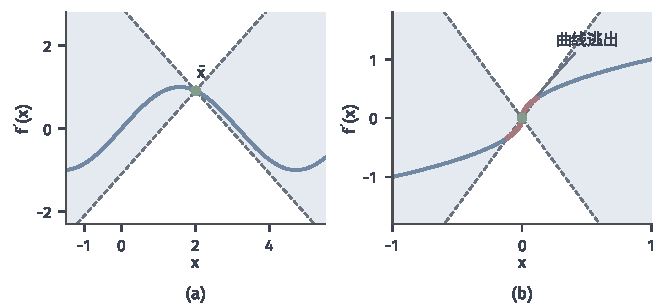
\includegraphics[width=112mm]{figures/05-optimization/02-smooth-optimization/matplotlib/smooth-gradient-cone/figure.pdf}
  \caption{梯度Lipschitz条件的几何含义。蓝线是导数曲线，浅蓝区域是从绿点出发、斜率为$\pm L$的双锥。(a)$f'(x)=\sin x$，取$L=1$，顶点放在$\bar{x}=2$，曲线留在锥内；顶点放在其他点时同样如此。(b)$f'(x)=\operatorname{sign}(x)\lvert x\rvert^{1/2}$，取$L=3$，顶点放在$0$，红色部分$\lvert x\rvert<1/9$逃出了锥；$L$再大，逃出的部分只是变短，永远存在。}
  \label{fig:smooth-gradient-cone}
\end{BookInlineFigure}

\paragraph{三个相近的条件}
“可微”“梯度连续”“梯度Lipschitz”是逐步加强的三个要求，图~\ref{fig:smooth-gradient-cone}(b)的函数正好落在中间。取$f(x)=\frac23\lvert x\rvert^{3/2}$，它处处可微，导数是
\[
 f'(x)=\operatorname{sign}(x)\lvert x\rvert^{1/2},
\]
这个导数也连续。但以$0$为参照点，
\[
 \frac{\lvert f'(x)-f'(0)\rvert}{\lvert x\rvert}=\lvert x\rvert^{-1/2},
\]
$x\to0$时趋于无穷，所以包含原点的任何区间上都没有光滑常数。

高阶可微也不能保证全局的常数。$f(x)=x^4$无穷次可微，而
\[
 \frac{\lvert f'(u)-f'(0)\rvert}{\lvert u\rvert}=4u^2,
\]
$u$变大时无界。限制在$[-R,R]$上时，$f''(x)=12x^2\leq12R^2$，常数$12R^2$随区域变大。所以说一个目标“光滑”时，要同时交代常数和它成立的区域。

\paragraph{下降引理}
有了坡度的限速，就能控制线性预测的误差。思路是把有限的位移分成无穷多小段累加：每一小段上的真实变化由该处的坡度决定，它与起点坡度之差不超过限速乘以已走的距离。

\begin{lemma}[下降引理]
\label{lem:smooth-descent}
设$f:\mathbb{R}^n\to\mathbb{R}$可微，并在集合$\bm{U}$上$L$光滑。若线段$\{\bm{x}+s\bm{p}:s\in[0,1]\}$落在$\bm{U}$中，则
\begin{equation}
 \bigl\lvert f(\bm{x}+\bm{p})-f(\bm{x})-\langle\nabla f(\bm{x}),\bm{p}\rangle\bigr\rvert
 \leq\frac{L}{2}\lVert\bm{p}\rVert_2^2.
 \label{eq:smooth-remainder}
\end{equation}
特别地，
\begin{equation}
 f(\bm{x}+\bm{p})\leq f(\bm{x})+\langle\nabla f(\bm{x}),\bm{p}\rangle+\frac{L}{2}\lVert\bm{p}\rVert_2^2.
 \label{eq:smooth-descent-lemma}
\end{equation}
\end{lemma}

\begin{proof}
令$\phi(s)=f(\bm{x}+s\bm{p})$，$s\in[0,1]$。由链式法则，
\[
 \phi'(s)=\langle\nabla f(\bm{x}+s\bm{p}),\bm{p}\rangle.
\]
线段在$\bm{U}$中，$\nabla f$沿线段Lipschitz，所以$\phi'$连续，微积分基本定理给出
\[
 f(\bm{x}+\bm{p})-f(\bm{x})=\int_0^1\langle\nabla f(\bm{x}+s\bm{p}),\bm{p}\rangle\,\mathrm{d}s.
\]

两边减去常数$\langle\nabla f(\bm{x}),\bm{p}\rangle$，并把它也写成$s$从$0$到$1$的积分，得到
\[
 f(\bm{x}+\bm{p})-f(\bm{x})-\langle\nabla f(\bm{x}),\bm{p}\rangle
 =\int_0^1\langle\nabla f(\bm{x}+s\bm{p})-\nabla f(\bm{x}),\bm{p}\rangle\,\mathrm{d}s.
\]

由Cauchy--Schwarz不等式和式~\eqref{eq:smooth-lipschitz}，被积函数的绝对值满足
\[
 \bigl\lvert\langle\nabla f(\bm{x}+s\bm{p})-\nabla f(\bm{x}),\bm{p}\rangle\bigr\rvert
 \leq Ls\lVert\bm{p}\rVert_2^2.
\]
对$s$从$0$积分到$1$，右端成为$\frac{L}{2}\lVert\bm{p}\rVert_2^2$，式~\eqref{eq:smooth-remainder}成立。去掉绝对值取上半部分，即得式~\eqref{eq:smooth-descent-lemma}。
\end{proof}

上界~\eqref{eq:smooth-descent-lemma}称为\term{下降引理}（descent lemma），它是后面证明目标下降的主要工具。把右端看成$\bm{p}$的函数，记作
\begin{equation}
 m_L(\bm{p})=f(\bm{x})+\langle\nabla f(\bm{x}),\bm{p}\rangle+\frac{L}{2}\lVert\bm{p}\rVert_2^2.
 \label{eq:smooth-upper-model}
\end{equation}
这是一个在当前点与$f$相切、开口向上的二次函数，像一只倒扣过来的碗从上方盖住了$f$。下半部分则是开口向下的二次函数，从下方托住$f$。

图~\ref{fig:smooth-upper-lower-model}画出$f(x)=1-\cos x$的情形。这里$f''(x)=\cos x$，取值在$[-1,1]$内，$L=1$，当前点$x^{(0)}=2$。整条曲线都夹在两条抛物线之间。

\begin{BookInlineFigure}
  \centering
  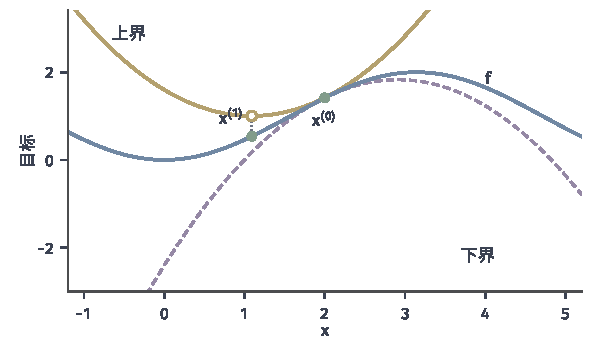
\includegraphics[width=100mm]{figures/05-optimization/02-smooth-optimization/matplotlib/smooth-upper-lower-model/figure.pdf}
  \caption{$f(x)=1-\cos x$在$x^{(0)}=2$处的二次上界（黄线）与二次下界（紫色虚线），$L=1$。空心点是上界的最低点，其正下方的绿点$x^{(1)}=2-\sin2$是目标在同一位置的真实值，后者不高于前者。}
  \label{fig:smooth-upper-lower-model}
\end{BookInlineFigure}

\paragraph{上界怎样限制一步更新}
上界的用途在于，它把“走到哪里”变成一个能解的问题。式~\eqref{eq:smooth-upper-model}对$\bm{p}$求梯度并令其为零，最低点是
\[
 \bm{p}=-\frac{1}{L}\nabla f(\bm{x}).
\]

代回式~\eqref{eq:smooth-descent-lemma}，得到一步能够保证的下降量：
\begin{equation}
 f\Bigl(\bm{x}-\frac{1}{L}\nabla f(\bm{x})\Bigr)\leq f(\bm{x})-\frac{1}{2L}\lVert\nabla f(\bm{x})\rVert_2^2.
 \label{eq:smooth-model-min}
\end{equation}

这个结论的意思是：只要落点在碗的最低处，真实目标不会比碗底更高。在图~\ref{fig:smooth-upper-lower-model}的例子里，$\sin2\approx0.909$，当前值、碗底值和真实落点值分别是
\[
 f(2)\approx1.416,\qquad m_L(-0.909)\approx1.003,\qquad f(1.091)\approx0.538.
\]
保证的下降量是$0.413$，实际下降$0.878$。上界不紧，但它不需要试探就能给出保证。

回到例~\eqref{eq:smooth-running}。此时$L=9$，当前点的上界最低点是$\bm{x}^{(1)}=(9,1)-\frac19(9,9)=(8,0)$，碗底高度与真实值分别是
\[
 f(\bm{x}^{(0)})-\frac{\lVert\bm{g}^{(0)}\rVert_2^2}{2L}=45-9=36,\qquad f(\bm{x}^{(1)})=32.
\]
图~\ref{fig:smooth-isotropic-model}显示了这一步的几何。上界的等高线是圆，真实目标的等高线是椭圆。经过当前点的圆完全落在经过当前点的椭圆之内，所以圆内每一点都比当前点低。

\begin{BookInlineFigure}
  \centering
  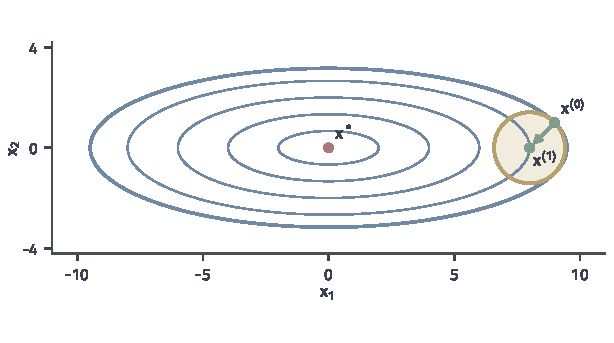
\includegraphics[width=104mm]{figures/05-optimization/02-smooth-optimization/matplotlib/smooth-isotropic-model/figure.pdf}
  \caption{各向同性的上界盖住各向异性的目标。蓝线是例~\eqref{eq:smooth-running}的等高线，粗线经过$\bm{x}^{(0)}$。黄圆是上界$m_L$经过$\bm{x}^{(0)}$的等高线，圆心$\bm{x}^{(1)}=(8,0)$是上界的最低点，绿色箭头是步$-\bm{g}^{(0)}/L$。圆的半径是$\lVert\bm{g}^{(0)}\rVert_2/L=\sqrt2$，比到最优解的距离小得多。}
  \label{fig:smooth-isotropic-model}
\end{BookInlineFigure}

这个图也说明了上界的弱点。它只知道一个数$L$，必须按最陡的方向处处提防，所以朝平坦的$x_1$方向也不敢多走。碗的类比到这里就要打折扣：真实地形是一条长谷，而这只碗是圆的，它保证安全，却不描述谷的走向。

\paragraph{局部模型能信多远}
下降引理有一句前提：线段要落在$L$成立的区域内。这句话不能省。取$f(x)=x^4$，当前点$x^{(0)}=1$，导数是$4$。在$[-1,1]$上$f''\leq12$，取$L=12$，上界是
\[
 m(x)=1+4(x-1)+6(x-1)^2.
\]

上界与目标之差可以因式分解，
\[
 f(x)-m(x)=(x-1)^3(x+3).
\]
当$-3\leq x\leq1$时它不大于零，上界盖得住；当$x>1$或$x<-3$时它大于零，上界失效。

图~\ref{fig:smooth-model-range}(b)放大了当前点附近：只要向右走一点点，$f''$就超过$12$，上界立刻盖不住。向左，上界一直盖到$x=-3$，比$L$成立的区间$[-1,1]$更远，因为靠近当前点那段曲率小于$12$，积累的余量抵消了后来过大的曲率。引理只承诺线段在区域内时成立，区域外可能成立，也可能不成立。

\begin{BookInlineFigure}
  \centering
  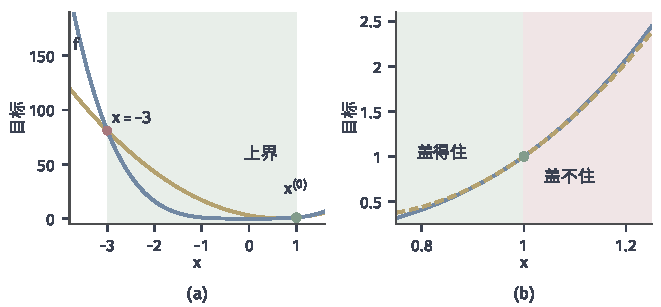
\includegraphics[width=112mm]{figures/05-optimization/02-smooth-optimization/matplotlib/smooth-model-range/figure.pdf}
  \caption{局部常数的有效范围。$f(x)=x^4$（蓝线），在$x^{(0)}=1$处用$[-1,1]$上的常数$L=12$作上界（黄线）。(a)浅绿区域$[-3,1]$内上界盖住目标，$x=-3$是另一个交点。(b)放大当前点附近：左侧盖得住；右侧浅红区域$f''>12$，上界立刻盖不住，虚线低于蓝线。}
  \label{fig:smooth-model-range}
\end{BookInlineFigure}

\paragraph{上界与凸性无关}
上界$m_L$永远是凸函数，这容易让人以为$L$光滑带有某种凸性。其实两件事互不蕴含。$L$限制的是弯曲的绝对大小，凸性限制的是弯曲的方向。表~\ref{tab:smooth-vs-convex}用四个一元函数列出全部组合。

\begin{BookInlineTable}
  \centering
  \begin{tabular}{@{}lll@{}}
    \toprule
     & 凸 & 非凸\\
    \midrule
    全局$L$光滑 & $x^2/2$，$L=1$ & $1-\cos x$，$L=1$\\
    无全局常数 & $x^4$ & $x^4-x^2$\\
    \bottomrule
  \end{tabular}
  \caption{全局光滑性与凸性互不蕴含。第一行的函数二阶导数有界，第二行无界；第一列的函数二阶导数非负，第二列会取负值。}
  \label{tab:smooth-vs-convex}
\end{BookInlineTable}

两者对局部模型的贡献也不同。光滑性给出二次上界，告诉我们一步最多变差多少，由此保证下降。凸性把式~\eqref{eq:smooth-remainder}的下半部分从开口向下的抛物线提高到切平面，也就是第~\ref{chap:optimization}章的支撑不等式，由此才能从一点的信息推断全局。$1-\cos x$在$x^{(0)}=3$附近上界依然成立，但这里的小梯度不说明接近最小点。

\paragraph{下水平集上的常数}
实际目标常常没有全局的$L$，例如$x^4$。好在下降算法不必到处走：只要每步都不升高，迭代点就留在初始的下水平集里。下面的引理说明，$L$只在下水平集上成立时，只要步长受限，这一步的整条线段就不会走出去，下降引理可以照用。

\begin{lemma}[梯度步留在下水平集内]
\label{lem:smooth-sublevel}
设$f:\mathbb{R}^n\to\mathbb{R}$可微，$\bm{S}=\{\bm{z}:f(\bm{z})\leq a\}$，$f$在$\bm{S}$上$L$光滑，$L>0$。设$\bm{x}\in\bm{S}$，$\bm{g}=\nabla f(\bm{x})\neq\bm{0}$，$0<\alpha<2/L$。则线段$\{\bm{x}-s\bm{g}:s\in[0,\alpha]\}$落在$\bm{S}$内，并且
\begin{equation}
 f(\bm{x}-\alpha\bm{g})\leq f(\bm{x})-\alpha\Bigl(1-\frac{L\alpha}{2}\Bigr)\lVert\bm{g}\rVert_2^2.
 \label{eq:smooth-sublevel-step}
\end{equation}
\end{lemma}

\begin{proof}
令$\phi(s)=f(\bm{x}-s\bm{g})$。设$\bar{s}$是使$\phi$在$[0,\bar{s}]$上始终不超过$a$的最大的$\bar{s}\in[0,\alpha]$，由连续性，这个最大值取得到。因为$\phi'(0)=-\lVert\bm{g}\rVert_2^2<0$且$\phi(0)\leq a$，所以$\bar{s}>0$。

线段$\{\bm{x}-s\bm{g}:s\in[0,\bar{s}]\}$在$\bm{S}$中，对$\bm{p}=-\bar{s}\bm{g}$用下降引理，得到
\[
 \phi(\bar{s})\leq f(\bm{x})-\bar{s}\Bigl(1-\frac{L\bar{s}}{2}\Bigr)\lVert\bm{g}\rVert_2^2<f(\bm{x})\leq a.
\]
严格不等式成立，是因为$0<\bar{s}<2/L$。

若$\bar{s}<\alpha$，由$\phi(\bar{s})<a$和连续性，$\phi$在$\bar{s}$右侧一小段上仍不超过$a$，与$\bar{s}$的取法矛盾。所以$\bar{s}=\alpha$，上面的不等式就是式~\eqref{eq:smooth-sublevel-step}。
\end{proof}

用$f(x)=x^4$、$x^{(0)}=1$核对一下。取$a=1$，$\bm{S}=[-1,1]$，$L=12$，于是$\alpha<1/6$时引理适用。取$\alpha=1/12$，走到$x=2/3$，式~\eqref{eq:smooth-sublevel-step}给出的上界和真实值分别是
\[
 1-\frac{1}{12}\cdot\frac12\cdot16=\frac13,\qquad f\Bigl(\frac23\Bigr)=\frac{16}{81}\approx0.198.
\]
若取$\alpha=1/2$，超出了范围，迭代在$1$和$-1$之间来回跳，目标不再下降。

\paragraph{目标差控制梯度}
式~\eqref{eq:smooth-model-min}还有一个推论。设$f$在$\mathbb{R}^n$上$L$光滑，并且下有界，记$f_{\inf}=\inf f$。式~\eqref{eq:smooth-model-min}的左端不低于$f_{\inf}$，移项得到
\begin{equation}
 \frac{1}{2L}\lVert\nabla f(\bm{x})\rVert_2^2\leq f(\bm{x})-f_{\inf}.
 \label{eq:smooth-gap-gradient}
\end{equation}
第~\ref{chap:optimization}章在强凸的条件下证过同样的不等式，这里既不要求凸，也不要求二阶可微，甚至不要求最优解存在。直观上，若坡度很陡而离下界很近，沿坡度走一步就会跌破下界。

\paragraph{用Hessian估计光滑常数}
定义~\ref{def:smooth-lipschitz}要比较所有点对，直接检验并不方便。目标二阶可微时，梯度的变化率就是Hessian，常数可以从Hessian读出。

\begin{theorem}[Hessian与光滑常数]
\label{thm:smooth-hessian}
设$\bm{U}\subseteq\mathbb{R}^n$是凸开集，$f$在$\bm{U}$上二阶连续可微。则$f$在$\bm{U}$上$L$光滑，当且仅当对所有$\bm{z}\in\bm{U}$，
\begin{equation}
 \lVert\nabla^2f(\bm{z})\rVert_2\leq L.
 \label{eq:smooth-hessian-bound}
\end{equation}
\end{theorem}

\begin{proof}
先设式~\eqref{eq:smooth-hessian-bound}成立。对$\bm{u},\bm{v}\in\bm{U}$，线段留在$\bm{U}$中，这里用到了$\bm{U}$的凸性。沿线段对梯度积分，得到
\[
 \nabla f(\bm{u})-\nabla f(\bm{v})=\int_0^1\nabla^2f\bigl(\bm{v}+s(\bm{u}-\bm{v})\bigr)(\bm{u}-\bm{v})\,\mathrm{d}s.
\]
取范数，积分的范数不超过范数的积分，被积向量的范数不超过$L\lVert\bm{u}-\bm{v}\rVert_2$，即得式~\eqref{eq:smooth-lipschitz}。

反过来，设$f$在$\bm{U}$上$L$光滑。取$\bm{z}\in\bm{U}$和单位向量$\bm{v}$，$s>0$充分小时$\bm{z}+s\bm{v}\in\bm{U}$，于是
\[
 \Bigl\lVert\frac{\nabla f(\bm{z}+s\bm{v})-\nabla f(\bm{z})}{s}\Bigr\rVert_2\leq L.
\]
令$s\downarrow0$，左端趋于$\lVert\nabla^2f(\bm{z})\bm{v}\rVert_2$。对所有单位向量取上确界，即得式~\eqref{eq:smooth-hessian-bound}。
\end{proof}

定理说明，最小的光滑常数恰好是$\bm{U}$上$\lVert\nabla^2f\rVert_2$的上确界。对称矩阵的谱范数等于特征值绝对值的最大者，定义与性质可参考\BookChapterRef{chap:eigen-spectral-decomposition}{卷二第6章“谱分解”}。要注意绝对值：负曲率同样计入$L$，例如$\frac12(x_1^2-4x_2^2)$的$L=4$。

几个常见情形可以直接写出。二次目标$\frac12\bm{x}^\top\bm{H}\bm{x}$的$L=\max_i\lvert\lambda_i(\bm{H})\rvert$，例~\eqref{eq:smooth-running}中$L=9$。最小二乘$\frac12\lVert\bm{A}\bm{x}-\bm{b}\rVert_2^2$的Hessian是$\bm{A}^\top\bm{A}$，所以$L=\lVert\bm{A}\rVert_2^2$。第~\ref{chap:optimization}章的二次拟合实例，Hessian的特征值是$2+\gamma$和$\gamma$，所以$L=2+\gamma$。

非二次目标要在整个区域上取上确界。考虑
\[
 f(\bm{x})=\cos(x_1+x_2)+\frac12\lVert\bm{x}\rVert_2^2,
\]
记$c=\cos(x_1+x_2)$，Hessian是
\[
 \nabla^2f(\bm{x})=\bm{I}-c\begin{bmatrix}1&1\\1&1\end{bmatrix}.
\]
方向$(1,-1)$上的特征值是$1$，方向$(1,1)$上的特征值是$1-2c$。$c$取遍$[-1,1]$时，$1-2c$取遍$[-1,3]$，所以$L=3$。这个目标在$c>1/2$的区域非凸，却是全局$3$光滑的。

\paragraph{矩阵太大时怎样估计}
维数很大时，特征值不便精确算出。有两类办法，它们的方向相反。第一类给上界，只用矩阵的元素：对称矩阵$\bm{H}$的谱范数不超过最大的绝对行和$\lVert\bm{H}\rVert_\infty$，也不超过Frobenius范数$\lVert\bm{H}\rVert_{\mathrm{F}}$；半正定时还不超过迹。第二类给下界：从向量$\bm{v}$出发反复乘$\bm{H}$，这个做法称为幂迭代，再计算Rayleigh商$\bm{v}^\top\bm{H}\bm{v}/\bm{v}^\top\bm{v}$。它不需要写出矩阵，只要能算矩阵向量积。

下面的矩阵用来比较这两类估计：
\[
 \bm{H}=\begin{bmatrix}2&1&0\\1&3&1\\0&1&2\end{bmatrix}.
\]
它的特征值是$1,2,4$，所以$L=4$。三个上界分别是
\[
 \lVert\bm{H}\rVert_\infty=5,\qquad \lVert\bm{H}\rVert_{\mathrm{F}}=\sqrt{21}\approx4.58,\qquad \operatorname{tr}\bm{H}=7.
\]

幂迭代从$\bm{v}=(1,1,1)$出发，前三次的Rayleigh商是
\[
 \frac{11}{3}\approx3.667,\qquad \frac{171}{43}\approx3.977,\qquad \frac{2731}{683}\approx3.999.
\]
图~\ref{fig:smooth-hessian-estimates}把两类估计放在一起。上界偏保守，用它得到的步长偏小，但步长是安全的。幂迭代逼近得快，却总从下方接近真值，直接拿来算步长可能略微超出安全范围。实践中常把幂迭代的结果乘一个略大于$1$的系数。

\begin{BookInlineFigure}
  \centering
  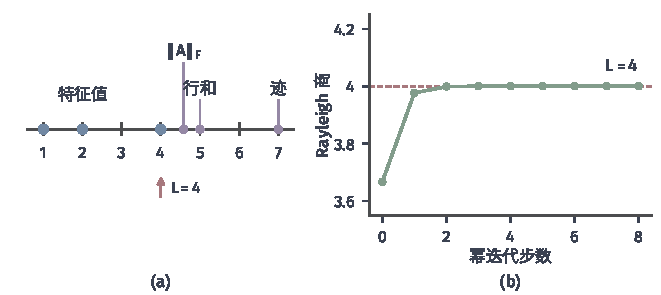
\includegraphics[width=112mm]{figures/05-optimization/02-smooth-optimization/matplotlib/smooth-hessian-estimates/figure.pdf}
  \caption{估计$L$的两类办法，矩阵见正文，特征值为$1,2,4$。(a)数轴上的蓝点是特征值，紫点是由元素算出的三个上界：Frobenius范数约$4.58$、最大绝对行和$5$、迹$7$，它们都不低于$L=4$。(b)幂迭代的Rayleigh商随步数增加，始终不超过$L$（红色虚线）。}
  \label{fig:smooth-hessian-estimates}
\end{BookInlineFigure}

对非二次目标，还要处理$\bm{z}$变化带来的麻烦：在一点上的估计并不代表整个区域。下一节的回溯线搜索正是为不知道$L$的情形准备的，它把估计常数换成了用真实函数值检验。

\section{步长的选择}
\label{sec:smooth-step-size}

现在固定当前点$\bm{x}$和一个下降方向$\bm{d}$，只决定走多远。记$\bm{g}=\nabla f(\bm{x})$，并把目标限制到这条射线上：
\begin{equation}
 \phi(\alpha)=f(\bm{x}+\alpha\bm{d}),\qquad \alpha\geq0.
 \label{eq:smooth-phi}
\end{equation}
由链式法则，
\[
 \phi'(\alpha)=\langle\nabla f(\bm{x}+\alpha\bm{d}),\bm{d}\rangle,\qquad \phi'(0)=\langle\bm{g},\bm{d}\rangle<0.
\]

候选步长满足什么条件，就可以接受？这个问题有三种回答，区别在于事先要知道什么、每一步要多算什么。固定步长事先靠$L$定好，运行时什么也不检验。回溯线搜索不需要$L$，用函数值检验每个候选。Wolfe条件再加上对方向导数的检验，换来更强的保证。

在二次目标上，$\phi$是一条抛物线，三种规则都可以写成步长的区间。设$f(\bm{x})=\frac12\bm{x}^\top\bm{H}\bm{x}$，$\bm{H}$对称正定，$\langle\bm{d},\bm{H}\bm{d}\rangle>0$。将$\phi$展开，得到
\[
 \phi(\alpha)=\phi(0)+\alpha\phi'(0)+\frac{\alpha^2}{2}\langle\bm{d},\bm{H}\bm{d}\rangle.
\]
它的最低点记作
\begin{equation}
 \alpha_{\mathrm{e}}=\frac{-\phi'(0)}{\langle\bm{d},\bm{H}\bm{d}\rangle}.
 \label{eq:smooth-exact-quadratic}
\end{equation}

用$\alpha_{\mathrm{e}}$改写，后面反复要用的两个式子是
\begin{equation}
 \begin{gathered}
 \phi(\alpha)=\phi(0)+\alpha\phi'(0)\Bigl(1-\frac{\alpha}{2\alpha_{\mathrm{e}}}\Bigr),\\
 \phi'(\alpha)=\phi'(0)\Bigl(1-\frac{\alpha}{\alpha_{\mathrm{e}}}\Bigr).
 \end{gathered}
 \label{eq:smooth-quadratic-line}
\end{equation}

例~\eqref{eq:smooth-running}从$\bm{x}^{(0)}$沿$\bm{d}=-\bm{g}^{(0)}=(-9,-9)$走时，下面三个数在本节一直用到：
\[
 \phi'(0)=-162,\qquad \langle\bm{d},\bm{H}\bm{d}\rangle=810,\qquad \alpha_{\mathrm{e}}=\frac15.
\]
这条线上的目标是
\[
 \phi(\alpha)=45-162\alpha+405\alpha^2.
\]

\subsection{固定步长}
\label{sec:smooth-fixed-step}

\paragraph{负梯度方向}
先看最简单的情形：$\bm{d}=-\bm{g}$，步长是事先定好的常数。在下降引理~\eqref{eq:smooth-descent-lemma}中取$\bm{p}=-\alpha\bm{g}$，得到
\begin{equation}
 f(\bm{x}-\alpha\bm{g})\leq f(\bm{x})-\alpha\Bigl(1-\frac{L\alpha}{2}\Bigr)\lVert\bm{g}\rVert_2^2.
 \label{eq:smooth-gd-step}
\end{equation}

括号前的$\alpha$是沿坡度得到的收益，括号里的$L\alpha/2$是弯曲带来的折扣。只要$0<\alpha<2/L$，保证的下降量就是正的。保证的下降量是$\alpha$的二次函数，在$\alpha=1/L$处最大，值为$\lVert\bm{g}\rVert_2^2/(2L)$，这就是式~\eqref{eq:smooth-model-min}。

图~\ref{fig:smooth-step-upper-bound}在例~\eqref{eq:smooth-running}上比较上界与真实目标。$L=9$，$\lVert\bm{g}^{(0)}\rVert_2^2=162$，上界是
\[
 45-162\alpha+729\alpha^2.
\]
取$\alpha=1/L=1/9$时，上界为$36$，真实值为$32$。上界在$\alpha=2/L$处回到$45$，真实目标却要到$\alpha=0.4$才回到$45$。

这个差别来自方向。这条线上目标的曲率是$810/162=5$，小于最坏方向的$9$。所以$2/L$并不是这个方向上真实的界限，而是对所有点、所有方向都安全的界限。

\begin{BookInlineFigure}
  \centering
  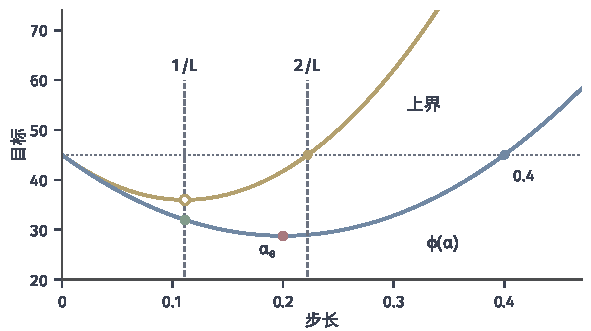
\includegraphics[width=100mm]{figures/05-optimization/02-smooth-optimization/matplotlib/smooth-step-upper-bound/figure.pdf}
  \caption{沿负梯度的一维剖面，例~\eqref{eq:smooth-running}，$\bm{x}^{(0)}=(9,1)$。蓝线是真实的$\phi(\alpha)$，黄线是下降引理的上界，点线是当前高度$45$。上界的最低点在$1/L$，回到$45$的位置是$2/L$；真实目标的最低点是红点$\alpha_{\mathrm{e}}=0.2$，回到$45$的位置是$0.4$。绿点是$\alpha=1/L$时的真实值，它低于同一步长的上界值（空心点）。}
  \label{fig:smooth-step-upper-bound}
\end{BookInlineFigure}

\paragraph{界限$2/L$在最坏方向上是紧的}
一元二次目标$f(x)=\frac{L}{2}x^2$说明，范围不能放宽。更新$x^+=x-\alpha Lx=(1-\alpha L)x$，乘数的绝对值小于$1$当且仅当$0<\alpha<2/L$。$\alpha=2/L$时乘数是$-1$，迭代来回跳；$\alpha>2/L$时迭代发散。

对二次目标，每个特征方向各自按这个规律变化。例~\eqref{eq:smooth-running}中$\bm{H}$是对角阵，固定步长的迭代逐分量写出来是
\[
 x_1^{(t+1)}=(1-\alpha)x_1^{(t)},\qquad x_2^{(t+1)}=(1-9\alpha)x_2^{(t)}.
\]
图~\ref{fig:smooth-fixed-paths}比较三个步长。$\alpha=1/9$时第二个乘数为零，一步消去最陡的分量，此后沿平坦方向每步只缩小到$8/9$。$\alpha=1/5$时两个乘数是$0.8$和$-0.8$，大小相同，路径锯齿前进。$\alpha=1/4$超过了$2/L=2/9$，第二个乘数是$-1.25$，$x_2$振荡发散。

\begin{BookInlineFigure}
  \centering
  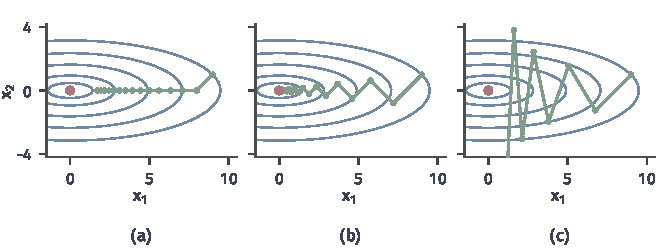
\includegraphics[width=112mm]{figures/05-optimization/02-smooth-optimization/matplotlib/smooth-fixed-paths/figure.pdf}
  \caption{例~\eqref{eq:smooth-running}上固定步长的梯度下降路径，绿点是迭代点，红点是最优解。(a)$\alpha=1/9$，乘数为$8/9$和$0$。(b)$\alpha=1/5$，乘数为$0.8$和$-0.8$。(c)$\alpha=1/4>2/L$，乘数为$0.75$和$-1.25$，路径沿$x_2$方向越摆越大。}
  \label{fig:smooth-fixed-paths}
\end{BookInlineFigure}

\paragraph{已知上界时怎样选}
若手里有一个上界$\hat{L}\geq L$，取$\alpha=1/\hat{L}$总是安全的。代入式~\eqref{eq:smooth-gd-step}，并用$L/\hat{L}\leq1$，得到
\[
 f(\bm{x})-f(\bm{x}-\alpha\bm{g})\geq\frac{1}{2\hat{L}}\lVert\bm{g}\rVert_2^2.
\]
上界放大几倍，保证的下降量就缩小几倍，这是高估的代价。低估的代价可能更严重：$\hat{L}<L/2$时$\alpha>2/L$，最坏方向上会发散。例~\eqref{eq:smooth-running}若误取$\hat{L}=4$，得到的恰是图~\ref{fig:smooth-fixed-paths}(c)。

固定步长的运行过程只有一步：算梯度，走$\alpha$，再算梯度。它每轮只读一次梯度，不计算函数值，也不做任何检验，这是它最大的优点。目标只在下水平集上有常数时，引理~\ref{lem:smooth-sublevel}说明用$\bm{S}=\{f\leq f(\bm{x}^{(0)})\}$上的$L$就够了；每步下降保证迭代留在$\bm{S}$内，同一个常数可以一直用。

\paragraph{一般下降方向}
后面各章的方向不一定是负梯度，上面的区间不能照搬。在下降引理中取$\bm{p}=\alpha\bm{d}$，得到
\begin{equation}
 f(\bm{x}+\alpha\bm{d})\leq f(\bm{x})+\alpha\langle\bm{g},\bm{d}\rangle+\frac{L\alpha^2}{2}\lVert\bm{d}\rVert_2^2.
 \label{eq:smooth-direction-bound}
\end{equation}

右端是$\alpha$的二次函数。它低于$f(\bm{x})$的范围、取最小值的步长分别是
\begin{equation}
 0<\alpha<\frac{2\lvert\langle\bm{g},\bm{d}\rangle\rvert}{L\lVert\bm{d}\rVert_2^2},\qquad
 \alpha=\frac{\lvert\langle\bm{g},\bm{d}\rangle\rvert}{L\lVert\bm{d}\rVert_2^2}.
 \label{eq:smooth-direction-range}
\end{equation}

代入后，一步保证的下降量可以用$\bm{d}$与$-\bm{g}$的夹角$\theta$表示：
\begin{equation}
 \frac{\langle\bm{g},\bm{d}\rangle^2}{2L\lVert\bm{d}\rVert_2^2}=\frac{\cos^2\theta}{2L}\lVert\bm{g}\rVert_2^2,
 \qquad\cos\theta=\frac{\lvert\langle\bm{g},\bm{d}\rangle\rvert}{\lVert\bm{g}\rVert_2\lVert\bm{d}\rVert_2}.
 \label{eq:smooth-cos-decrease}
\end{equation}

式~\eqref{eq:smooth-direction-range}含有方向的长度和方向导数，这两点都有具体后果。先看长度。把方向放大$10$倍，$\bm{d}=-10\bm{g}^{(0)}$，再取$\alpha=1/L=1/9$，实际位移是$-\frac{10}{9}\bm{g}^{(0)}$，于是
\[
 \bm{x}^{(1)}=(9,1)-10(1,1)=(-1,-9),\qquad f(\bm{x}^{(1)})=365.
\]
目标从$45$涨到$365$。图~\ref{fig:smooth-direction-scale}(a)的虚线正是这种情形。步长的单位包含了方向的长度，$1/L$只适用于$\bm{d}=-\bm{g}$这一个尺度。

\begin{BookInlineFigure}
  \centering
  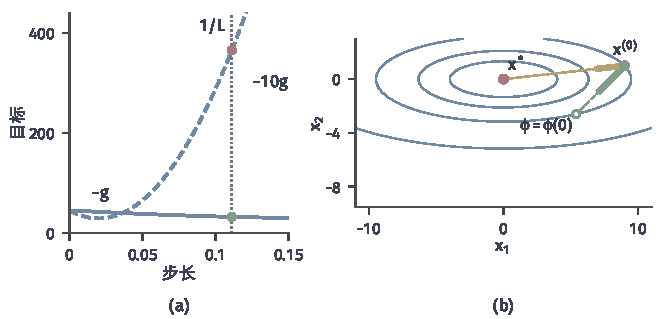
\includegraphics[width=112mm]{figures/05-optimization/02-smooth-optimization/matplotlib/smooth-direction-scale/figure.pdf}
  \caption{一般方向不能照搬$\alpha<2/L$。(a)沿$-\bm{g}$（实线）与$-10\bm{g}$（虚线）的目标剖面，同样取$\alpha=1/L$，前者到$32$，后者到$365$。(b)从$\bm{x}^{(0)}$出发的两个方向：绿色$-\bm{g}$，黄色$-\bm{H}^{-1}\bm{g}$。粗线段是式~\eqref{eq:smooth-direction-range}保证下降的范围，虚线延伸到真实目标回到起始高度或到达最低点的位置。}
  \label{fig:smooth-direction-scale}
\end{BookInlineFigure}

再看方向导数。取$\bm{d}=(-1,0.9)$，它几乎贴着等高线，$\langle\bm{g}^{(0)},\bm{d}\rangle=-0.9$，$\lVert\bm{d}\rVert_2^2=1.81$，由式~\eqref{eq:smooth-cos-decrease}，保证的下降量是
\[
 \frac{0.81}{2\cdot9\cdot1.81}\approx0.025,
\]
而负梯度方向是$9$。方向虽然严格下降，贴着等高线走，保证的进展几乎没有。

第三个例子说明上界有时过于悲观。$\bm{d}=-\bm{H}^{-1}\bm{g}^{(0)}=(-9,-1)$时，式~\eqref{eq:smooth-direction-range}的范围是
\[
 0<\alpha<\frac{2\cdot90}{9\cdot82}\approx0.244.
\]
但这个方向直指最优解，$\alpha=1$一步到位。上界用的是最陡方向的曲率$9$，这条线上的实际曲率却只有
\[
 \frac{\langle\bm{d},\bm{H}\bm{d}\rangle}{\lVert\bm{d}\rVert_2^2}=\frac{90}{82}\approx1.1.
\]
图~\ref{fig:smooth-direction-scale}(b)的黄色粗线段远短于黄色虚线，差的就是这个比值。

这三个例子都说明，固定步长依赖对$L$和方向尺度的先验知识。下一小节改用实际目标值检验候选。

\subsection{回溯线搜索}
\label{sec:smooth-backtracking}

\paragraph{主要思想}
不知道$L$时，不妨先迈一大步，看看真实高度是否令人满意；不满意就退回来，迈小一些。这里的关键是“满意”的标准。只要求$\phi(\alpha)<\phi(0)$是不够的，后面会看到，这样的下降可能小到不产生进展。

合理的标准是把实际下降与一阶预测比较。走$\alpha$时，线性预测的下降量是$-\alpha\phi'(0)$。我们要求实际下降不少于预测的固定比例。这和记账相似：线性预测是承诺的收益，实际下降是到账的收益，至少到账一定比例才算数。

\begin{definition}[Armijo条件]
\label{def:smooth-armijo}
设$\langle\bm{g},\bm{d}\rangle<0$，$c_1\in(0,1)$。若步长$\alpha>0$满足
\begin{equation}
 f(\bm{x}+\alpha\bm{d})\leq f(\bm{x})+c_1\alpha\langle\bm{g},\bm{d}\rangle,
 \label{eq:smooth-armijo}
\end{equation}
就说它满足\term{Armijo条件}（Armijo condition），也称\term{充分下降条件}（sufficient decrease condition）。
\end{definition}

条件的右端是从$(0,\phi(0))$出发、斜率为$c_1\phi'(0)$的直线，它比切线平缓。Armijo条件要求曲线落在这条直线下方。$c_1$的两个端点都不能取：$c_1=0$退化成只要求下降，$c_1=1$时直线就是切线，而凸的$\phi$永远不低于切线，没有步长可以通过。实践中常取很小的值，如$c_1=10^{-4}$\scite{math-nocedal2006numerical}。

由式~\eqref{eq:smooth-quadratic-line}，二次目标上的Armijo条件化为$1-\alpha/(2\alpha_{\mathrm{e}})\geq c_1$，也就是
\begin{equation}
 0<\alpha\leq2(1-c_1)\alpha_{\mathrm{e}}.
 \label{eq:smooth-armijo-quadratic}
\end{equation}
例中取$c_1=0.1$，可接受的步长是$(0,0.36]$，如图~\ref{fig:smooth-armijo}中的绿色线段。

\begin{BookInlineFigure}
  \centering
  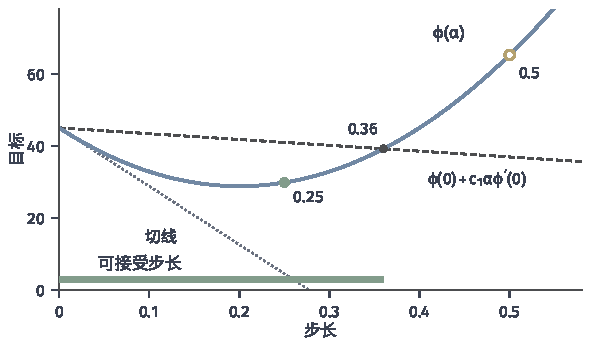
\includegraphics[width=100mm]{figures/05-optimization/02-smooth-optimization/matplotlib/smooth-armijo/figure.pdf}
  \caption{Armijo条件，例~\eqref{eq:smooth-running}第一轮，$c_1=0.1$。蓝线是$\phi(\alpha)$，点线是切线，深灰虚线是斜率为$c_1\phi'(0)$的检验直线，曲线在它下方的步长（绿色线段）$(0,0.36]$可接受。回溯从$\alpha=1$开始（$\phi(1)=288$，在图外），$\alpha=0.5$被拒绝（空心点），$\alpha=0.25$通过（绿点）。}
  \label{fig:smooth-armijo}
\end{BookInlineFigure}

这样的做法称为\term{回溯线搜索}（backtracking line search）：从初始试探步长$\alpha_0$开始，不满足式~\eqref{eq:smooth-armijo}就乘以缩减因子$\rho\in(0,1)$，第一个通过的步长就是结果。下面的定理回答这个过程为什么会停，以及停在多大的步长上。

\begin{theorem}[回溯的终止与步长下界]
\label{thm:smooth-backtracking}
设$f$在$\bm{x}$处可微，$\langle\bm{g},\bm{d}\rangle<0$，$c_1,\rho\in(0,1)$，$\alpha_0>0$。则回溯经有限次试探后终止。

进一步设$\nabla f$在线段$\{\bm{x}+s\bm{d}:s\in[0,\alpha_0]\}$上以常数$L>0$满足式~\eqref{eq:smooth-lipschitz}，并记
\begin{equation}
 \bar{\alpha}=\frac{2(1-c_1)\lvert\langle\bm{g},\bm{d}\rangle\rvert}{L\lVert\bm{d}\rVert_2^2}.
 \label{eq:smooth-armijo-threshold}
\end{equation}
则$(0,\alpha_0]$中不超过$\bar{\alpha}$的步长都满足Armijo条件，接受的步长$\alpha$和试探次数$n$满足
\begin{equation}
 \alpha\geq\min\{\alpha_0,\rho\bar{\alpha}\},\qquad
 n\leq1+\Bigl\lceil\log_{1/\rho}\frac{\alpha_0}{\bar{\alpha}}\Bigr\rceil_+,
 \label{eq:smooth-backtracking-bounds}
\end{equation}
其中$\lceil a\rceil_+=\max\{\lceil a\rceil,0\}$。一步的下降量满足
\begin{equation}
 f(\bm{x})-f(\bm{x}+\alpha\bm{d})\geq c_1\min\{\alpha_0,\rho\bar{\alpha}\}\lvert\langle\bm{g},\bm{d}\rangle\rvert.
 \label{eq:smooth-backtracking-decrease}
\end{equation}
\end{theorem}

\begin{proof}
先证终止。由可微性，当$\alpha\downarrow0$时
\[
 \frac{\phi(\alpha)-\phi(0)}{\alpha}\to\phi'(0).
\]
因为$\phi'(0)<0$且$c_1<1$，所以$\phi'(0)<c_1\phi'(0)$。于是存在$\alpha'>0$，使$\alpha\in(0,\alpha']$时差商小于$c_1\phi'(0)$，这正是式~\eqref{eq:smooth-armijo}。试探步长$\alpha_0\rho^{j}$趋于零，有限步后落入$(0,\alpha']$。

再证定量部分。设$\alpha\in(0,\alpha_0]$，$\alpha\leq\bar{\alpha}$。线段上的Lipschitz条件使式~\eqref{eq:smooth-direction-bound}成立。由$\alpha\leq\bar{\alpha}$得到
\[
 \frac{L\alpha}{2}\lVert\bm{d}\rVert_2^2\leq(1-c_1)\lvert\langle\bm{g},\bm{d}\rangle\rvert.
\]
代入式~\eqref{eq:smooth-direction-bound}的最后一项，得到
\[
 f(\bm{x}+\alpha\bm{d})\leq f(\bm{x})+\alpha\langle\bm{g},\bm{d}\rangle+\alpha(1-c_1)\lvert\langle\bm{g},\bm{d}\rangle\rvert.
\]
由$\langle\bm{g},\bm{d}\rangle<0$，右端等于式~\eqref{eq:smooth-armijo}的右端。

若$\alpha_0$直接通过，则$\alpha=\alpha_0$。否则，被接受步长的上一次试探$\alpha/\rho$未通过，由刚证的结论$\alpha/\rho>\bar{\alpha}$，所以$\alpha>\rho\bar{\alpha}$。这得到步长下界。

第$j$次试探的步长是$\alpha_0\rho^{j-1}$，它一旦不超过$\bar{\alpha}$就一定通过，这要求$j-1\geq\log_{1/\rho}(\alpha_0/\bar{\alpha})$，试探次数的上界由此得出。把步长下界代入式~\eqref{eq:smooth-armijo}，即得式~\eqref{eq:smooth-backtracking-decrease}。
\end{proof}

定理中各条件的作用可以分开看。下降方向是必需的：若$\phi'(0)>0$，式~\eqref{eq:smooth-armijo}对所有充分小的$\alpha$都不成立，回溯不会在小步长上停下来。终止只用到当前点的可微性，算法也不需要知道$L$。$L$只出现在分析里，用来定量说明步长不会太小。

这里的$L$只要覆盖试探过的线段，这就是局部光滑性足够的原因。取$f(x)=x^4$，它没有全局的$L$，从$x=1.5$出发，$d=-13.5$，$c_1=0.1$，$\rho=1/2$，$\alpha_0=1$。试探点和目标值依次是
\[
 \begin{aligned}
 \alpha=1:&\quad x=-12,\quad f=20736,\\
 \alpha=\tfrac12:&\quad x=-5.25,\quad f\approx759.7,\\
 \alpha=\tfrac14:&\quad x=-1.875,\quad f\approx12.36,\\
 \alpha=\tfrac18:&\quad x=-0.1875,\quad f\approx0.0012.
 \end{aligned}
\]
最后一次的右端是$5.0625-0.1\cdot\frac18\cdot182.25\approx2.78$，条件满足。用固定步长时必须事先想清楚区域和常数，回溯把这些问题都交给了实际的函数值。

\paragraph{计算过程}
下面用例~\eqref{eq:smooth-running}走一遍，方向取负梯度，这也是下一章梯度下降法使用的形式。

\needspace{6\baselineskip}
\paragraph{变量}
\begin{itemize}
 \item $\bm{x}\in\mathbb{R}^n$：当前点；$\bm{g}\in\mathbb{R}^n$：当前梯度；$\bm{d}\in\mathbb{R}^n$：方向。
 \item $f_{\mathrm{cur}}$：当前目标值；$\sigma=\langle\bm{g},\bm{d}\rangle$：方向导数，是一个负数。
 \item $\alpha$：当前试探步长；$c_1,\rho,\alpha_0$：Armijo常数、缩减因子、初始试探步长。
 \item $\varepsilon$：梯度容差。
\end{itemize}

\paragraph{初始化}
取定初始点，算出它的目标值和梯度。例中$\bm{x}=(9,1)$，参数和初值是
\[
 c_1=0.1,\quad\rho=0.5,\quad\alpha_0=1,\quad\varepsilon=10^{-3},
\]
\[
 f_{\mathrm{cur}}=45,\quad\bm{g}=(9,9).
\]

\needspace{6\baselineskip}
\paragraph{每轮更新}
\begin{enumerate}
 \item 计算方向$\bm{d}=-\bm{g}$和方向导数$\sigma=-\lVert\bm{g}\rVert_2^2$。令$\alpha\leftarrow\alpha_0$。

 例中第一轮$\bm{d}=(-9,-9)$，$\sigma=-162$，$\alpha=1$。

 \item 计算试探点$\bm{x}+\alpha\bm{d}$及其目标值，按式~\eqref{eq:smooth-armijo}与$f_{\mathrm{cur}}+c_1\alpha\sigma$比较。不满足就令$\alpha\leftarrow\rho\alpha$，重复这一步。

 例中第一轮的三次试探依次是
 \[
 \begin{aligned}
 \alpha=1:&\quad(0,-8),\quad f=288>28.8,\\
 \alpha=0.5:&\quad(4.5,-3.5),\quad f=65.25>36.9,\\
 \alpha=0.25:&\quad(6.75,-1.25),\quad f=29.8125\leq40.95.
 \end{aligned}
 \]
 第三次通过。

 \item 接受试探点，更新$\bm{x}$、$f_{\mathrm{cur}}$，计算新梯度。

 例中得到
 \[
 \bm{x}=(6.75,-1.25),\quad f_{\mathrm{cur}}=29.8125,\quad\bm{g}=(6.75,-11.25).
 \]

 \item 若$\lVert\bm{g}\rVert_2\leq\varepsilon$，停止；否则回到第1步。

 例中$\lVert\bm{g}\rVert_2\approx13.12$，继续。第二轮$\sigma=-172.125$，试探如下：
 \[
 \begin{aligned}
 \alpha=1:&\quad(0,10),\quad f=450>12.6,\\
 \alpha=0.5:&\quad(3.375,4.375),\quad f\approx91.83>21.21,\\
 \alpha=0.25:&\quad(5.0625,1.5625),\quad f\approx23.80\leq25.51.
 \end{aligned}
 \]
\end{enumerate}

后面几轮的结果列在表~\ref{tab:smooth-backtrack-run}中，路径见图~\ref{fig:smooth-backtrack-path}。第一轮接受的$0.25$超过了固定步长的安全上限$2/L=2/9$，这正是检验真实函数值带来的好处。

\begin{BookInlineTable}
  \centering
  \begin{tabular}{@{}rrrrrrr@{}}
    \toprule
    $t$ & $x_1^{(t)}$ & $x_2^{(t)}$ & $f(\bm{x}^{(t)})$ & $\lVert\bm{g}^{(t)}\rVert_2$ & 试探次数 & $\alpha^{(t)}$\\
    \midrule
    0 & 9.000 & 1.000 & 45.000 & 12.728 & 3 & 0.25\\
    1 & 6.750 & $-1.250$ & 29.813 & 13.120 & 3 & 0.25\\
    2 & 5.063 & 1.563 & 23.801 & 14.946 & 4 & 0.125\\
    3 & 4.430 & $-0.195$ & 9.983 & 4.766 & 2 & 0.5\\
    4 & 2.215 & 0.684 & 4.556 & 6.539 & 4 & 0.125\\
    5 & 1.938 & $-0.085$ & 1.911 & 2.085 & 2 & 0.5\\
    6 & 0.969 & 0.299 & 0.872 & 2.861 & 4 & 0.125\\
    \bottomrule
  \end{tabular}
  \caption{例~\eqref{eq:smooth-running}上负梯度方向的回溯，$c_1=0.1$，$\rho=0.5$，$\alpha_0=1$。每行是该轮开始时的点，以及该轮的试探次数与接受的步长。}
  \label{tab:smooth-backtrack-run}
\end{BookInlineTable}

\begin{BookInlineFigure}
  \centering
  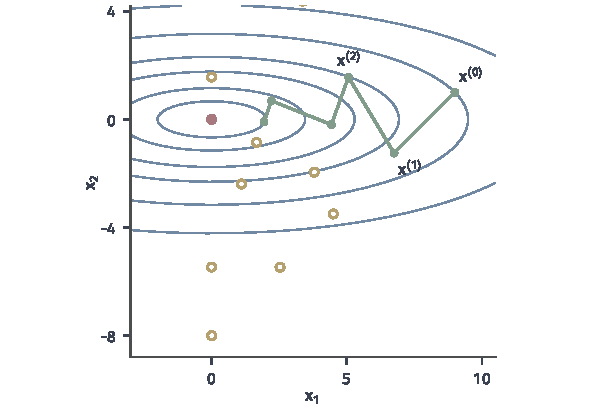
\includegraphics[width=100mm]{figures/05-optimization/02-smooth-optimization/matplotlib/smooth-backtrack-path/figure.pdf}
  \caption{回溯的路径。绿点和绿线是前五轮接受的点，黄色空心点是这几轮被拒绝的试探点，它们都落在比当前点差得多的位置，超出图幅的未画出。目标见例~\eqref{eq:smooth-running}，参数同表~\ref{tab:smooth-backtrack-run}。}
  \label{fig:smooth-backtrack-path}
\end{BookInlineFigure}

从$t=3$起步长在$0.5$与$0.125$之间交替：沿平坦方向时能迈大步，碰到陡峭分量时又缩回来。迭代在$\lVert\bm{g}\rVert_2\leq10^{-3}$时结束，共$25$轮、$76$次试探。最终得到
\[
 \bm{x}^{(25)}\approx(4.98\times10^{-4},\,-2.2\times10^{-5}),\qquad f(\bm{x}^{(25)})\approx1.3\times10^{-7}.
\]

\paragraph{每次试探增加的函数计算}
回溯的代价是被拒绝的试探。一轮共试探$n$次，就多算$n$次函数值。由式~\eqref{eq:smooth-backtracking-bounds}，例中第一轮的$\bar{\alpha}=0.2$，试探次数的上界是$1+\lceil\log_25\rceil=4$，实际是$3$次。

每轮都从同一个$\alpha_0$开始，就要反复支付同样的试探。一个自然的办法是用上一轮接受的步长作起点，也就是$\alpha_0^{(t+1)}=\alpha^{(t)}$。这时步长不增，设$\nabla f$全局$L$光滑、方向为负梯度，则每次拒绝都发生在$\alpha>\bar{\alpha}=2(1-c_1)/L$的步长上。每次拒绝让步长缩小$\rho$倍，所以全程被拒绝的总次数$R$满足
\begin{equation}
 R\leq1+\log_{1/\rho}\frac{\alpha_0L}{2(1-c_1)}.
 \label{eq:smooth-total-rejections}
\end{equation}
这样，函数计算的总次数是$T+R$，也就是只比轮数多一个对数项。例中上界约是$3.3$，全程实际拒绝$3$次。

但是步长只减不增，走到平坦的区域也不能放大。折中的办法是每轮把初值放大$1/\rho$倍。取$\rho=1/2$时，第$t$轮被拒绝$r_t$次，步长变化是
\[
 \alpha^{(t+1)}=2\cdot2^{-r_{t+1}}\alpha^{(t)}.
\]
累加后，只要步长有正的下界，$\sum_tr_t$至多比$T$多一个常数，所以每轮平均约试探两次。图~\ref{fig:smooth-backtrack-cost}中，每轮从$1$开始时平均$3.04$次，放大策略平均$2.06$次。

\begin{BookInlineFigure}
  \centering
  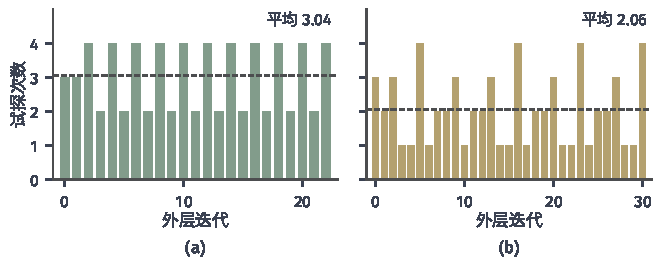
\includegraphics[width=112mm]{figures/05-optimization/02-smooth-optimization/matplotlib/smooth-backtrack-cost/figure.pdf}
  \caption{每轮的试探次数，直到目标差不超过$10^{-6}$，目标见例~\eqref{eq:smooth-running}。(a)每轮都从$\alpha_0=1$开始，共$23$轮、$70$次试探。(b)每轮的初值取上一轮接受步长的$2$倍，共$31$轮、$64$次试探。虚线是平均值。}
  \label{fig:smooth-backtrack-cost}
\end{BookInlineFigure}

试探的单价也可以压低。例如最小二乘$\frac12\lVert\bm{A}\bm{x}-\bm{b}\rVert_2^2$，只要算一次$\bm{A}\bm{d}$，每个候选的目标值就是$\frac12\lVert\bm{r}+\alpha\bm{A}\bm{d}\rVert_2^2$，其中$\bm{r}=\bm{A}\bm{x}-\bm{b}$，只需向量运算。通过的试探点的函数值和部分中间量也常能在计算下一轮梯度时复用。

\subsection{Wolfe条件}
\label{sec:smooth-wolfe}

\paragraph{只看函数值挡不住太小的步长}
Armijo条件只限制步长不能太大，太小的步长总能通过。回溯之所以没有这个问题，是因为被接受的步长的上一次试探失败过，$\alpha$不会比门槛小太多。可一旦步长不是由回溯产生，比如来自插值或其他公式，这层保护就没有了。

下面的例子中，每一步都满足Armijo条件，迭代却停在非驻点。取$f(x)=x^2$，方向恒为$d=-1$，步长$\alpha^{(t)}=2^{-t-1}$，于是
\[
 x^{(t)}=1+2^{-t}\to1.
\]

一步的实际下降量和预测下降量分别是
\[
 2^{-t-1}\bigl(2+3\cdot2^{-t-1}\bigr),\qquad 2^{-t-1}\bigl(2+2^{1-t}\bigr).
\]
括号比较可知，$c_1\leq3/4$时Armijo条件每一步都成立。但极限点$x=1$处$f'(1)=2\neq0$，迭代不是因为到了谷底才停下，只是步子缩得太快。图~\ref{fig:smooth-short-steps}(a)画出了这个序列。

\begin{BookInlineFigure}
  \centering
  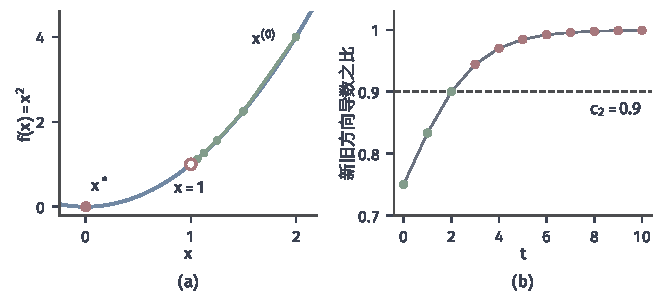
\includegraphics[width=112mm]{figures/05-optimization/02-smooth-optimization/matplotlib/smooth-short-steps/figure.pdf}
  \caption{只满足Armijo条件的序列可能停在非驻点。(a)$f(x)=x^2$上的序列$x^{(t)}=1+2^{-t}$（绿点），收敛到空心红点$x=1$，真正的最优解是实心红点。(b)每步新旧方向导数之比。比值超过虚线$c_2=0.9$的点（红色）不满足曲率条件。}
  \label{fig:smooth-short-steps}
\end{BookInlineFigure}

\paragraph{用斜率判断“还能走”}
步子太短的后果，可以从落脚点的坡度看出来。如果落脚后$\phi'(\alpha)$仍然和$\phi'(0)$差不多陡，说明继续往前走还有几乎同样的下降率，停下来可惜。反之，坡度已经明显变缓甚至变正，才说明这段路的收益基本取尽了。用上面的例子算比值：
\[
 \frac{\phi'(\alpha^{(t)})}{\phi'(0)}=\frac{2+2^{-t}}{2+2^{1-t}}\to1.
\]
落脚点的坡度几乎不变，这正是步长太短的标志，见图~\ref{fig:smooth-short-steps}(b)。

\begin{definition}[Wolfe条件]
\label{def:smooth-wolfe}
设$\langle\bm{g},\bm{d}\rangle<0$，$0<c_1<c_2<1$。若$\alpha>0$满足Armijo条件~\eqref{eq:smooth-armijo}和
\begin{equation}
 \langle\nabla f(\bm{x}+\alpha\bm{d}),\bm{d}\rangle\geq c_2\langle\bm{g},\bm{d}\rangle,
 \label{eq:smooth-curvature}
\end{equation}
就说它满足\term{Wolfe条件}（Wolfe conditions）；式~\eqref{eq:smooth-curvature}单独称为\term{曲率条件}（curvature condition）。若把式~\eqref{eq:smooth-curvature}换成
\begin{equation}
 \bigl\lvert\langle\nabla f(\bm{x}+\alpha\bm{d}),\bm{d}\rangle\bigr\rvert\leq c_2\lvert\langle\bm{g},\bm{d}\rangle\rvert,
 \label{eq:smooth-strong-curvature}
\end{equation}
就说它满足\term{强Wolfe条件}（strong Wolfe conditions）。
\end{definition}

曲率条件只限制方向导数不能太负，也就是挡住太短的步长；Armijo条件挡住太长的步长；两者一上一下。强条件还限制方向导数不能太正，因而在最低点附近形成一个窗口。

在二次目标上，由式~\eqref{eq:smooth-quadratic-line}，方向导数之比是$1-\alpha/\alpha_{\mathrm{e}}$，两种条件的区间可以直接写出：
\begin{equation}
 \begin{aligned}
 \text{Wolfe：}&\quad(1-c_2)\alpha_{\mathrm{e}}\leq\alpha\leq2(1-c_1)\alpha_{\mathrm{e}},\\
 \text{强Wolfe：}&\quad(1-c_2)\alpha_{\mathrm{e}}\leq\alpha\leq\min\{1+c_2,\,2(1-c_1)\}\alpha_{\mathrm{e}}.
 \end{aligned}
 \label{eq:smooth-wolfe-quadratic}
\end{equation}

例~\eqref{eq:smooth-running}第一轮，$\alpha_{\mathrm{e}}=0.2$，取$c_1=0.1$，$c_2=0.5$。Wolfe区间是$[0.1,0.36]$，强Wolfe区间是$[0.1,0.3]$。代入三个候选步长检验，其中$c_2\phi'(0)=-81$：
\[
 \begin{aligned}
 \alpha=0.05:&\quad\phi'=-121.5<-81,\ \text{太短，不通过};\\
 \alpha=0.25:&\quad\phi'=40.5,\ \text{两种条件都通过};\\
 \alpha=0.33:&\quad\phi'=105.3,\ \text{Wolfe通过，强Wolfe不通过}.
 \end{aligned}
\]

图~\ref{fig:smooth-wolfe-intervals}换了一个非凸的一元剖面。Armijo条件的可接受集是一个长区间；加上曲率条件后，靠近$0$的太短步长被去掉；强条件再去掉斜率太大的部分，只留下每个谷底、谷间凸起附近的小窗口。这里的窗口不止一个，线搜索只需要落进其中之一。

\begin{BookInlineFigure}
  \centering
  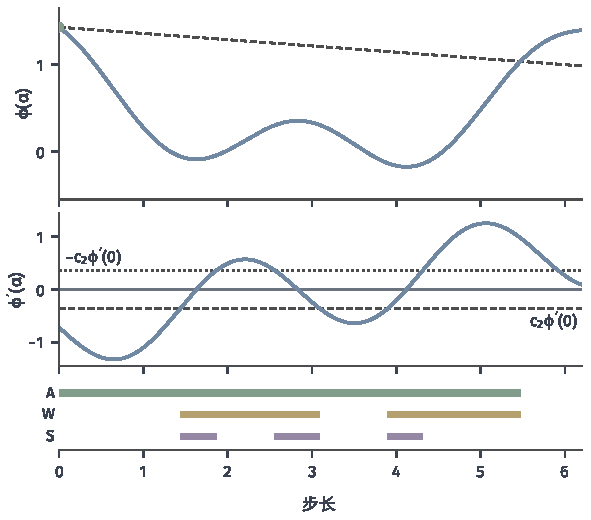
\includegraphics[width=100mm]{figures/05-optimization/02-smooth-optimization/matplotlib/smooth-wolfe-intervals/figure.pdf}
  \caption{非凸剖面$\phi(\alpha)=0.12(\alpha-3)^2+0.35\cos(2.2\alpha)$上的可接受步长，$c_1=0.1$，$c_2=0.5$。上图虚线是Armijo检验直线，中图的虚线和点线是$\pm c_2\phi'(0)$。下方三条：A是满足Armijo条件的步长，W是满足Wolfe条件的步长，S是满足强Wolfe条件的步长。}
  \label{fig:smooth-wolfe-intervals}
\end{BookInlineFigure}

\paragraph{满足条件的步长存在}
要使用这些条件，先要确认可接受的步长总是存在。需要的额外假设是$\phi$有下界；否则沿这条线可以无限下降，不存在要停下的理由。

\begin{theorem}[Wolfe步长的存在]
\label{thm:smooth-wolfe-existence}
设$f$连续可微，$\langle\bm{g},\bm{d}\rangle<0$，$\phi$在$[0,\infty)$上有下界，$0<c_1<c_2<1$。则存在一个开区间，其中每个步长都满足强Wolfe条件，因而也满足Wolfe条件。
\end{theorem}

\begin{proof}
直线$\ell(\alpha)=\phi(0)+c_1\alpha\phi'(0)$无下界，而$\phi$有下界，所以两者在某个正步长相交。因$\phi'(0)<c_1\phi'(0)$，$\alpha$很小时$\phi<\ell$。记最小的正交点为$\alpha'$，于是在$(0,\alpha')$上$\phi<\ell$。

由微分中值定理，存在$\alpha''\in(0,\alpha')$，使
\[
 \phi'(\alpha'')=\frac{\phi(\alpha')-\phi(0)}{\alpha'}=c_1\phi'(0).
\]

因为$0<c_1<c_2$且$\phi'(0)<0$，$\alpha''$处同时有
\[
 \phi'(\alpha'')>c_2\phi'(0),\qquad \lvert\phi'(\alpha'')\rvert<c_2\lvert\phi'(0)\rvert.
\]
$\phi'$连续，这两个严格不等式在$\alpha''$的一个邻域内保持；邻域取得足够小时留在$(0,\alpha')$中，Armijo条件也严格成立。
\end{proof}

定理保证了存在，算法还要把这样的步长找出来。满足Wolfe条件的一个简单办法是二分。维护区间$[\alpha_{\mathrm{lo}},\alpha_{\mathrm{hi}}]$，初值为$[0,\infty)$，用一个试探点$\alpha$：Armijo不满足，就令$\alpha_{\mathrm{hi}}=\alpha$；Armijo满足而曲率条件不满足，就令$\alpha_{\mathrm{lo}}=\alpha$；两者都满足则接受。新试探点取区间中点，上端还是无穷时取$2\alpha_{\mathrm{lo}}$。

这个过程有限步终止。假如一直不停，且$\alpha_{\mathrm{hi}}$始终是无穷，则$\alpha_{\mathrm{lo}}\to\infty$且都满足Armijo条件，推出$\phi\to-\infty$，与下界矛盾。

否则区间缩到一点$\alpha_\infty$。由端点的Armijo状态，$\phi(\alpha_{\mathrm{hi}})$在直线上方，$\phi(\alpha_{\mathrm{lo}})$在直线下方，两者作差商后取极限，得到$\phi'(\alpha_\infty)\geq c_1\phi'(0)$。另一方面$\alpha_{\mathrm{lo}}$不满足曲率条件，取极限得到$\phi'(\alpha_\infty)\leq c_2\phi'(0)$。于是
\[
 c_1\phi'(0)\leq\phi'(\alpha_\infty)\leq c_2\phi'(0).
\]
而$c_1<c_2$、$\phi'(0)<0$说明$c_2\phi'(0)<c_1\phi'(0)$，矛盾。

用例子走两次。从$\alpha=1$开始时，$1$和$0.5$都不满足Armijo条件，上端缩到$0.5$，试探$0.25$，两个条件都满足，接受。从$\alpha=0.05$开始时，Armijo满足，曲率条件不满足，下端更新为$0.05$，上端还是无穷，试探$0.1$，它恰好落在Wolfe区间的左端点上，接受。强Wolfe条件要用更细致的分段放大与缩小程序，每轮通常只需很少几次试探，具体写法可查阅\scite{math-nocedal2006numerical}。

\paragraph{Wolfe条件怎样避免步长过小}
下面的定理把“不会太小”写成定量结论，并给出它累积起来的效果。这里只要求当前点和接受点之间满足Lipschitz条件。

\begin{theorem}[Wolfe步长的下界与累积下降]
\label{thm:smooth-wolfe-decrease}
设步长$\alpha$满足Wolfe条件，$\bm{x}$与$\bm{x}+\alpha\bm{d}$这一对点满足以$L$为常数的式~\eqref{eq:smooth-lipschitz}。则
\begin{equation}
 \alpha\geq\frac{(1-c_2)\lvert\langle\bm{g},\bm{d}\rangle\rvert}{L\lVert\bm{d}\rVert_2^2},
 \label{eq:smooth-wolfe-lower}
\end{equation}
\begin{equation}
 f(\bm{x})-f(\bm{x}+\alpha\bm{d})\geq\frac{c_1(1-c_2)}{L}\cos^2\theta\,\lVert\bm{g}\rVert_2^2,
 \label{eq:smooth-wolfe-decrease}
\end{equation}
其中$\theta$是$\bm{d}$与$-\bm{g}$的夹角。若$f$下有界，且迭代的每一步都满足上述假设，则
\begin{equation}
 \sum_{t=0}^{\infty}\cos^2\theta^{(t)}\,\lVert\bm{g}^{(t)}\rVert_2^2<\infty.
 \label{eq:smooth-zoutendijk}
\end{equation}
\end{theorem}

\begin{proof}
从曲率条件~\eqref{eq:smooth-curvature}两端减去$\langle\bm{g},\bm{d}\rangle$，得到
\[
 \langle\nabla f(\bm{x}+\alpha\bm{d})-\bm{g},\bm{d}\rangle\geq(c_2-1)\langle\bm{g},\bm{d}\rangle=(1-c_2)\lvert\langle\bm{g},\bm{d}\rangle\rvert.
\]

由Cauchy--Schwarz不等式和假设，左端不超过$L\alpha\lVert\bm{d}\rVert_2^2$，于是式~\eqref{eq:smooth-wolfe-lower}成立。

把式~\eqref{eq:smooth-wolfe-lower}代入Armijo条件~\eqref{eq:smooth-armijo}，一步下降量不小于
\[
 c_1\alpha\lvert\langle\bm{g},\bm{d}\rangle\rvert\geq\frac{c_1(1-c_2)}{L}\cdot\frac{\langle\bm{g},\bm{d}\rangle^2}{\lVert\bm{d}\rVert_2^2},
\]
再由$\cos\theta$的定义，即得式~\eqref{eq:smooth-wolfe-decrease}。

对$t=0,\ldots,T-1$累加，左端不超过$f(\bm{x}^{(0)})-\inf f$，与$T$无关。令$T\to\infty$，式~\eqref{eq:smooth-zoutendijk}成立。
\end{proof}

式~\eqref{eq:smooth-zoutendijk}称为\term{Zoutendijk条件}（Zoutendijk condition）。它把线搜索和方向分开：线搜索保证了这个级数收敛，方向只需不要越来越贴近等高线。若$\cos\theta^{(t)}\geq\delta>0$一直成立，就有$\lVert\bm{g}^{(t)}\rVert_2\to0$。回到图~\ref{fig:smooth-short-steps}的序列：那里$\cos\theta^{(t)}=1$，梯度却不趋于零，它违反的正是曲率条件。

下降量~\eqref{eq:smooth-wolfe-decrease}和式~\eqref{eq:smooth-cos-decrease}形式相同，只是常数不同。这说明Wolfe条件在不知道$L$的情况下，达到了和按$L$选步长同量级的保证。

\paragraph{拟牛顿曲率更新中的用途}
第~\ref{chap:quasi-newton}章的方法用相邻两点的梯度差来逼近曲率。设相邻两点的位移和梯度差是
\[
 \bm{s}=\alpha\bm{d},\qquad \bm{y}=\nabla f(\bm{x}+\alpha\bm{d})-\bm{g}.
\]
若要让对称正定矩阵$\bm{B}$满足$\bm{B}\bm{s}=\bm{y}$，两边与$\bm{s}$作内积，就得到必要条件
\[
 \langle\bm{s},\bm{y}\rangle=\langle\bm{s},\bm{B}\bm{s}\rangle>0.
\]

这个条件对非凸目标不会自动成立，而Wolfe条件恰好保证它。由曲率条件，
\begin{equation}
 \langle\bm{s},\bm{y}\rangle=\alpha\bigl(\phi'(\alpha)-\phi'(0)\bigr)\geq\alpha(1-c_2)\lvert\phi'(0)\rvert>0.
 \label{eq:smooth-wolfe-curvature-pair}
\end{equation}
这里只需要Wolfe条件，不需要强Wolfe条件。

用$f(x)=1-\cos x$、$x=2$、$d=-1$看两个步长，取$c_1=0.1$，$c_2=0.9$。此时$\phi'(0)=-\sin2\approx-0.909$。图~\ref{fig:smooth-secant-curvature}中，黄线和绿线对应下面的两个候选：
\[
 \begin{aligned}
 \alpha=0.4:&\quad\phi'(\alpha)\approx-1.000,\quad\langle\bm{s},\bm{y}\rangle\approx-0.036,\\
 \alpha=1.3:&\quad\phi'(\alpha)\approx-0.644,\quad\langle\bm{s},\bm{y}\rangle\approx0.345.
 \end{aligned}
\]
两者都满足Armijo条件。$\alpha=0.4$不满足曲率条件，得到的$\langle\bm{s},\bm{y}\rangle$是负的，不能用来更新正定矩阵；$\alpha=1.3$满足Wolfe条件，可以使用。

\begin{BookInlineFigure}
  \centering
  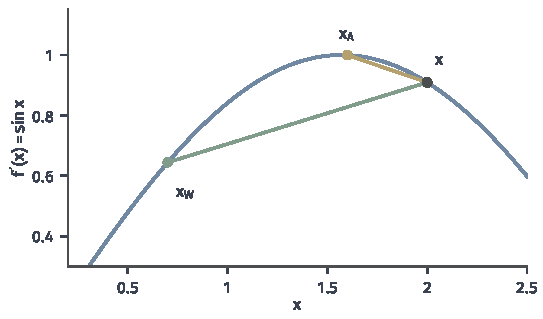
\includegraphics[width=92mm]{figures/05-optimization/02-smooth-optimization/matplotlib/smooth-secant-curvature/figure.pdf}
  \caption{曲率条件与割线斜率。蓝线是$f(x)=1-\cos x$的导数$\sin x$，深灰点是当前点$x=2$，沿$d=-1$移动。黄点$x_{\mathrm{A}}=1.6$只满足Armijo条件，割线斜率$y/s$为负。绿点$x_{\mathrm{W}}=0.7$满足Wolfe条件，割线斜率为正。}
  \label{fig:smooth-secant-curvature}
\end{BookInlineFigure}

\paragraph{非线性共轭梯度的下降分析中的用途}
强Wolfe条件的用处在另一类方法。第~\ref{chap:first-order-methods}章的非线性共轭梯度法把新方向取成新的负梯度加上旧方向的倍数。下面记新点的梯度为$\bm{g}_+$，系数为$\beta$：
\[
 \bm{d}_+=-\bm{g}_++\beta\bm{d}.
\]

新方向要是下降方向，需要检查它的方向导数：
\begin{equation}
 \langle\bm{g}_+,\bm{d}_+\rangle=-\lVert\bm{g}_+\rVert_2^2+\beta\langle\bm{g}_+,\bm{d}\rangle.
 \label{eq:smooth-cg-descent}
\end{equation}
第二项中的$\langle\bm{g}_+,\bm{d}\rangle$恰好是上一轮落脚点的方向导数。它若太大，加上$\beta$的放大可能抵消第一项，新方向就不再下降。Wolfe条件只限制它不能太负，对正的一侧不设限；强Wolfe条件才限制它的绝对值。

图~\ref{fig:smooth-cg-descent}用具体的向量说明差别。取$\bm{g}=(2,0)$，$\bm{d}=-\bm{g}$，系数取一种常见形式：
\[
 \beta=\frac{\lVert\bm{g}_+\rVert_2^2}{\lVert\bm{g}\rVert_2^2}.
\]

\begin{BookInlineFigure}
  \centering
  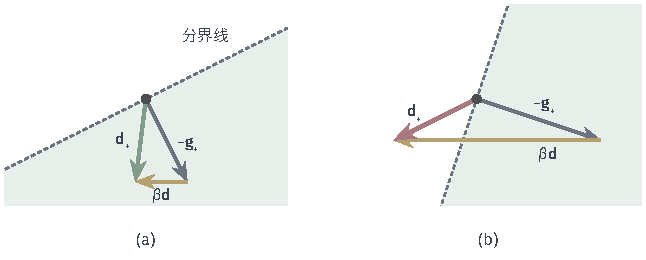
\includegraphics[width=108mm]{figures/05-optimization/02-smooth-optimization/tikz/smooth-cg-descent/figure.pdf}
  \caption{落脚点的方向导数决定新方向是否下降。浅绿区域是$\bm{g}_+$对应的下降半平面，虚线是分界线。旧方向$\bm{d}=(-2,0)$，灰色箭头是$-\bm{g}_+$，黄色箭头是$\beta\bm{d}$，两者之和是$\bm{d}_+$。(a)$\bm{g}_+=(-0.5,1)$，$\langle\bm{g}_+,\bm{d}\rangle=1$，绿色的$\bm{d}_+$留在半平面内。(b)$\bm{g}_+=(-3,1)$，$\langle\bm{g}_+,\bm{d}\rangle=6$，超过$\lvert\langle\bm{g},\bm{d}\rangle\rvert=4$，红色的$\bm{d}_+$落到半平面之外。}
  \label{fig:smooth-cg-descent}
\end{BookInlineFigure}

两种情形的数值分别是
\[
 \begin{aligned}
 \bm{g}_+=(-0.5,1):&\quad\beta=0.3125,\quad\langle\bm{g}_+,\bm{d}_+\rangle=-0.9375,\\
 \bm{g}_+=(-3,1):&\quad\beta=2.5,\quad\langle\bm{g}_+,\bm{d}_+\rangle=5.
 \end{aligned}
\]
后一种情形的新方向是上升方向。强Wolfe条件取$c_2<1$就排除了这种比值大于$1$的情况；要在所有轮次都保证下降，还需要对$c_2$的进一步限制和相应的$\beta$公式，这些在第~\ref{chap:first-order-methods}章讨论。常用参数也反映了这种分工：拟牛顿法常取$c_2=0.9$，非线性共轭梯度常取$c_2=0.1$\scite{math-nocedal2006numerical}。

\paragraph{精确线搜索：只作理论对照}
把窗口一直收紧，就得到\term{精确线搜索}（exact line search）：取$\phi$的最小点，至少满足
\begin{equation}
 \langle\nabla f(\bm{x}+\alpha\bm{d}),\bm{d}\rangle=0.
 \label{eq:smooth-exact-orthogonal}
\end{equation}
这是$c_2\to0$时强Wolfe条件的极限。此时式~\eqref{eq:smooth-cg-descent}的第二项消失，分析变得干净，所以理论推导常先考虑它。

二次目标上式~\eqref{eq:smooth-exact-quadratic}给出显式解。例~\eqref{eq:smooth-running}用精确步长，从形如$r(9,\pm1)$的点出发，一步到达$0.8r(9,\mp1)$，所以
\[
 \bm{x}^{(t)}=0.8^t\bigl(9,(-1)^t\bigr).
\]
下一轮的方向是下一轮的负梯度，式~\eqref{eq:smooth-exact-orthogonal}说明相邻方向互相垂直，于是路径成直角锯齿，如图~\ref{fig:smooth-exact-zigzag}。

\begin{BookInlineFigure}
  \centering
  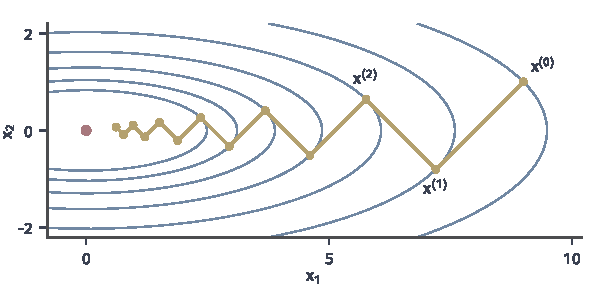
\includegraphics[width=100mm]{figures/05-optimization/02-smooth-optimization/matplotlib/smooth-exact-zigzag/figure.pdf}
  \caption{精确线搜索的路径。黄点是例~\eqref{eq:smooth-running}上负梯度方向取精确步长的迭代点，蓝线是经过这些点的等高线。每一段都在终点与等高线相切，相邻两段互相垂直，目标每轮乘以$0.64$。}
  \label{fig:smooth-exact-zigzag}
\end{BookInlineFigure}

“精确”并不等于最好。这个例子上精确线搜索每轮目标缩小到$0.64$倍，而下一节会看到，回溯用更少的轮数就达到了同样的精度。对一般目标，精确求解一维问题要多次函数或梯度计算，非凸时还要说明找的是哪个局部最小点。因此实际算法使用有限的接受条件，精确线搜索只作为分析时的对照。

\paragraph{三种规则的比较}
表~\ref{tab:smooth-step-rules}汇总本节的比较。比较的对象都是沿固定下降方向选步长，差别在事先要什么信息、每轮多算什么、换来什么保证。

\begin{table*}[!htbp]
  \centering
  \begin{tabular}{@{}llll@{}}
    \toprule
    规则 & 事先需要 & 每轮额外计算 & 保证\\
    \midrule
    固定步长 & $L$的上界，方向的尺度 & 无 & 式~\eqref{eq:smooth-gd-step}、\eqref{eq:smooth-cos-decrease}\\
    回溯（Armijo） & 下降方向，初始试探步长 & $n$次函数值 & 式~\eqref{eq:smooth-backtracking-decrease}\\
    Wolfe & $\phi$有下界 & 函数值和方向导数 & 式~\eqref{eq:smooth-wolfe-decrease}，$\langle\bm{s},\bm{y}\rangle>0$\\
    强Wolfe & 同上 & 同上，试探常更多 & 另限制落脚点方向导数的绝对值\\
    精确线搜索 & $\phi$的最小点可求 & 一维优化 & 落脚点方向导数为零\\
    \bottomrule
  \end{tabular}
  \caption{选择步长的规则。各行的保证都针对固定的下降方向，方向的质量由夹角$\theta$单独体现。}
  \label{tab:smooth-step-rules}
\end{table*}

\section{求解误差与计算成本}
\label{sec:smooth-accuracy-cost}

上一节比较的是单步。一个算法要迭代许多轮，两个算法之间的比较还要回答更多问题。这就需要回答：两种方法求解同一个问题，怎样比较才算数？第~\ref{chap:optimization}章规定了怎样衡量一个近似解，本节把它接到迭代过程上，再加上计算量的统计。

\paragraph{结论会随口径翻转}
在例~\eqref{eq:smooth-running}上，从$\bm{x}^{(0)}=(9,1)$出发，用五种步长规则运行负梯度方法，直到目标差不超过$10^{-6}$。表~\ref{tab:smooth-cost-run}列出外层轮数和各种读取次数。这里算总次数时把一次函数值、一次梯度、一次矩阵向量积各记为一个单位，因为对二次目标它们都要做一次矩阵向量积。

\begin{BookInlineTable}
  \centering
  \begin{tabular}{@{}lrrrrr@{}}
    \toprule
    步长规则 & 轮数$T$ & 函数值 & 梯度 & 矩阵向量积 & 总次数\\
    \midrule
    固定$\alpha=1/L$ & 75 & 0 & 76 & 0 & 76\\
    固定$\alpha=0.2$ & 40 & 0 & 41 & 0 & 41\\
    精确线搜索 & 40 & 0 & 41 & 40 & 81\\
    回溯，$\alpha_0=1$ & 23 & 71 & 24 & 0 & 95\\
    回溯，初值放大 & 31 & 65 & 32 & 0 & 97\\
    \bottomrule
  \end{tabular}
  \caption{例~\eqref{eq:smooth-running}上负梯度方法达到目标差不超过$10^{-6}$的计算量。固定步长$0.2=2/(L+\mu)$要同时知道$L$和$\mu$；梯度数包含初始点。回溯的函数值数包含初始点和所有被拒绝的试探。}
  \label{tab:smooth-cost-run}
\end{BookInlineTable}

按轮数看，回溯最少，比第二名少了将近一半。按总次数看，排序几乎反过来：回溯不如不做任何试探的固定步长，而精确线搜索也花掉了比固定步长$0.2$多一倍的计算。图~\ref{fig:smooth-cost-convergence}中两张图的曲线次序不同，差别只在横轴。

\begin{BookInlineFigure}
  \centering
  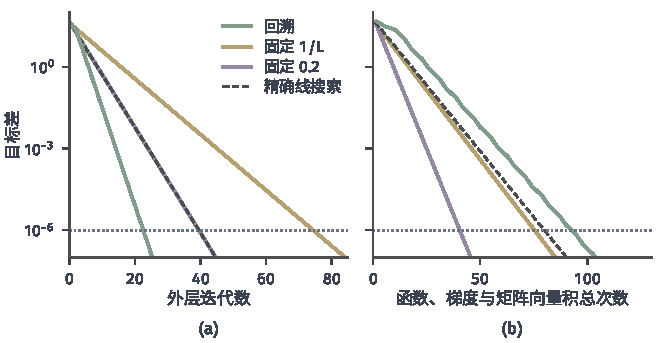
\includegraphics[width=112mm]{figures/05-optimization/02-smooth-optimization/matplotlib/smooth-cost-convergence/figure.pdf}
  \caption{同一组运行的两种横轴，目标见例~\eqref{eq:smooth-running}，纵轴是目标差，点线是$10^{-6}$。(a)横轴是外层迭代数，绿色的回溯最快。(b)横轴是函数值、梯度与矩阵向量积的总次数，紫色的固定步长$0.2$最快。回溯曲线在(b)中被试探次数拉长。}
  \label{fig:smooth-cost-convergence}
\end{BookInlineFigure}

这个例子不说明哪种规则更好。若函数值远比梯度便宜，或者$L$和$\mu$未知，结论都要改变。它说明的是：不交代口径的比较没有意义。比较之前要固定三件事：用什么量衡量误差，算法交出哪个点，计算量怎样累计。

\paragraph{误差标准}
第~\ref{chap:optimization}章的三种指标在这里要按问题类型选择。凸目标上驻点就是全局最优解，目标差$e_f=f(\bm{x})-f^\star$有明确的含义，比较时通常用它，保证也通常写成目标差的形式。

一般非凸目标的$f^\star$既算不出来，算法也无法保证接近它。这时能够断言的只有驻点残差$e_g=\lVert\nabla f(\bm{x})\rVert_2$：它只回答一阶条件差多少，不说明是局部还是全局的最小点，这在第~\ref{chap:saddle-points}章还要细分。

两种标准之间的换算，依据是第~\ref{chap:optimization}章三种误差的换算和本章的式~\eqref{eq:smooth-gap-gradient}。由目标差推梯度只要$L$：
\[
 e_g\leq\sqrt{2L\,e_f}.
\]
由梯度推目标差还要曲率下界$\mu$：
\[
 e_f\leq\frac{e_g^2}{2\mu}.
\]

例~\eqref{eq:smooth-running}中$L=9$，$\mu=1$。目标差$10^{-6}$只保证梯度不超过$\sqrt{18}\times10^{-3}\approx4.2\times10^{-3}$；梯度$10^{-3}$保证目标差不超过$5\times10^{-7}$。所以两种标准的“同样精度”并不相同，比较时不能混用。

\paragraph{一步下降怎样累积成驻点保证}
前面三种步长规则的下降保证都能写成同一个形式：一步的下降量不少于$c\lVert\bm{g}^{(t)}\rVert_2^2$，$c$是正常数。把这种形式累加起来，就得到不依赖凸性的驻点保证。

\begin{lemma}[累加下降]
\label{lem:smooth-telescoping}
设$f$下有界，$f_{\inf}=\inf f$，常数$c>0$，迭代满足
\begin{equation}
 f(\bm{x}^{(t)})-f(\bm{x}^{(t+1)})\geq c\lVert\bm{g}^{(t)}\rVert_2^2,\qquad t=0,\ldots,T-1.
 \label{eq:smooth-uniform-decrease}
\end{equation}
则
\begin{equation}
 \min_{0\leq t<T}\lVert\bm{g}^{(t)}\rVert_2^2\leq\frac{f(\bm{x}^{(0)})-f_{\inf}}{cT}.
 \label{eq:smooth-telescoping}
\end{equation}
\end{lemma}

\begin{proof}
对$t=0,\ldots,T-1$累加式~\eqref{eq:smooth-uniform-decrease}，左端相消，得到
\[
 f(\bm{x}^{(0)})-f(\bm{x}^{(T)})\geq c\sum_{t=0}^{T-1}\lVert\bm{g}^{(t)}\rVert_2^2\geq cT\min_{0\leq t<T}\lVert\bm{g}^{(t)}\rVert_2^2.
\]
左端不超过$f(\bm{x}^{(0)})-f_{\inf}$，移项即得。
\end{proof}

由式~\eqref{eq:smooth-telescoping}，要使$\min_t\lVert\bm{g}^{(t)}\rVert_2\leq\varepsilon$，轮数只要达到
\begin{equation}
 T\geq\frac{f(\bm{x}^{(0)})-f_{\inf}}{c\,\varepsilon^2}.
 \label{eq:smooth-iteration-bound}
\end{equation}

下一章将用这种累加结果处理一般非凸情形。三种规则对应的常数$c$如下，方向都取负梯度，Wolfe的情形允许夹角满足$\cos\theta^{(t)}\geq\delta>0$的一般方向，此时下降量与$\lVert\bm{g}^{(t)}\rVert_2^2$的比例同样有正下界：
\[
 \begin{aligned}
 \text{固定步长}\ \alpha=\tfrac{1}{L}:&\quad c=\frac{1}{2L},\\
 \text{回溯}:&\quad c=\min\Bigl\{c_1\alpha_0,\ \frac{2\rho c_1(1-c_1)}{L}\Bigr\},\\
 \text{Wolfe}:&\quad c=\frac{c_1(1-c_2)\delta^2}{L}.
 \end{aligned}
\]

代入例~\eqref{eq:smooth-running}的数值，看看这种保证和实际运行的距离。$f(\bm{x}^{(0)})-f_{\inf}=45$，$L=9$，取$\varepsilon=10^{-3}$。固定步长$1/L$的$c=1/18$，式~\eqref{eq:smooth-iteration-bound}要求$T\geq8.1\times10^8$，而实际只用了$78$轮。

差距这样大是因为式~\eqref{eq:smooth-telescoping}对任意$L$光滑的目标成立，包括最坏的非凸函数，它没有用到这个例子的二次结构。因此要区分两种“轮数”：理论界是对一类问题的最坏保证，实测值是在一个问题上的表现。两者都有用，但不能相互替代。

\paragraph{返回哪个迭代点}
式~\eqref{eq:smooth-telescoping}左端是历史上最小的梯度，所以保证的是某一轮的点，不一定是最后一轮。这个区别不是形式上的。取$f(x)=1-\cos x$，固定步长$\alpha=1/L=1$，从$x^{(0)}=3$出发。前四轮的迭代值如下：
\[
 \begin{aligned}
 x&:\ 3,\ 2.859,\ 2.580,\ 2.047,\ 1.159,\\
 f&:\ 1.990,\ 1.960,\ 1.846,\ 1.459,\ 0.600,\\
 \lvert f'\rvert&:\ 0.141,\ 0.279,\ 0.533,\ 0.889,\ 0.916.
 \end{aligned}
\]

目标在下降，梯度却在上升，如图~\ref{fig:smooth-best-vs-last}。起点靠近山顶$x=\pi$，那里梯度很小；离开山顶的过程中坡度越来越陡。由此可见，下降引理只控制目标的单调性，不控制梯度的单调性。

\begin{BookInlineFigure}
  \centering
  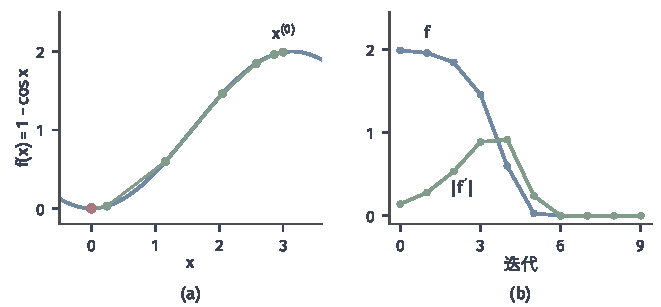
\includegraphics[width=112mm]{figures/05-optimization/02-smooth-optimization/matplotlib/smooth-best-vs-last/figure.pdf}
  \caption{目标单调下降时梯度可以先升后降。$f(x)=1-\cos x$，$\alpha=1$，$x^{(0)}=3$。(a)曲线上的迭代点（绿色）。(b)目标值（蓝）单调下降，导数绝对值（绿）在前四轮上升，到第$5$轮后才迅速下降。}
  \label{fig:smooth-best-vs-last}
\end{BookInlineFigure}

这个例子还有另一面：若容差取$\varepsilon=0.2$，初始点$x^{(0)}=3$本身就能通过检验，而它靠近的是极大点。所以驻点残差小只是一阶条件的说明，它不区分山顶与谷底。

报告结果时，常见的返回规则有三种。一是最后一轮$\bm{x}^{(T)}$，凸目标上的多数保证针对它，不需要记录历史。二是历史最佳，即目标值或梯度范数最小的那一轮，式~\eqref{eq:smooth-telescoping}对应这种规则，需要额外记录。三是停止点，第一次满足$\lVert\bm{g}^{(t)}\rVert_2\leq\varepsilon$的那一轮，停止时它就是历史上第一个合格的点。

下一章有些方法的目标值不单调，最后一轮不一定是最好的一轮，这时必须说明按哪条规则返回。

\paragraph{停止精度}
实际运行时$f^\star$未知，停止规则只能用可计算的量。梯度范数是首选，第~\ref{chap:optimization}章的相对标准，即把容差乘以$\max\{1,\lVert\bm{g}^{(0)}\rVert_2\}$，能够避免目标整体缩放带来的问题。步长或目标变化量太小的检验只能作辅助：回溯在一轮中接受了很小的步长时，位移也很小，但这只反映这一轮的步长，并不说明点已接近驻点。

容差还要与计算机的能力相称。在双精度浮点数中，$1+\delta$对$\delta$小于约$1.1\times10^{-16}$的数等于$1$。考虑$f(x)=1+\frac12x^2$，$x=10^{-9}$时，真实值$1+5\times10^{-19}$与$1$无法区分。

因此在最优值附近，比较函数值只能把点确定到约$\sqrt{\text{机器精度}}\approx10^{-8}$的范围，Armijo检验也就失去了分辨力。梯度$f'(x)=x$却还能算准。这说明可达到的精度取决于用什么量作判断，容差设得比判断量的计算误差还小是没有意义的。

\paragraph{总计算量}
选定误差标准和返回规则后，记$T(\varepsilon)$为达到精度$\varepsilon$所需的外层轮数。总计算量要把每一轮实际做过的所有运算加起来。设一次函数值、梯度、矩阵向量积的代价分别是$c_f,c_g,c_{\mathrm{mv}}$，第$t$轮有$n^{(t)}$次函数计算、$k^{(t)}$次内层矩阵向量积、线性代数运算量$c_{\mathrm{la}}^{(t)}$，于是
\begin{equation}
 W(\varepsilon)=\sum_{t=0}^{T(\varepsilon)-1}\Bigl(n^{(t)}c_f+c_g+k^{(t)}c_{\mathrm{mv}}+c_{\mathrm{la}}^{(t)}\Bigr).
 \label{eq:smooth-total-work}
\end{equation}

式中$n^{(t)}$包含被拒绝的试探；$k^{(t)}$是用迭代法解内层线性方程时的步数。图~\ref{fig:smooth-work-accounting}显示了每一轮的三部分怎样累加成$W(\varepsilon)$。

\begin{BookInlineFigure}
  \centering
  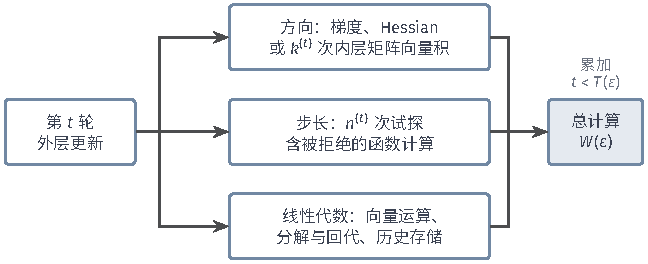
\includegraphics[width=108mm]{figures/05-optimization/02-smooth-optimization/tikz/smooth-work-accounting/figure.pdf}
  \caption{总计算量的组成。每一轮外层更新包含方向计算、步长试探和线性代数三部分，对达到精度所需的全部轮次累加，得到$W(\varepsilon)$。迭代轮数只决定累加的项数，每项的大小要另外统计。}
  \label{fig:smooth-work-accounting}
\end{BookInlineFigure}

\paragraph{单次更新的代价}
不同方法的每轮代价差别很大。表~\ref{tab:smooth-per-iter}按$n$维稠密问题列出下一章起要用到的几类操作。其中第三行的方向要解线性方程$\bm{H}\bm{d}=-\bm{g}$：可以分解矩阵直接解，也可以用迭代法只做矩阵向量积、解到一定精度为止，后者就是内层求解。

\begin{BookInlineTable}
  \centering
  \begin{tabular}{@{}lll@{}}
    \toprule
    一轮更新的操作 & 运算量 & 存储\\
    \midrule
    梯度与向量更新 & $c_g+O(n)$ & $O(n)$\\
    回溯线搜索 & 再加$n^{(t)}c_f$ & $O(n)$\\
    分解Hessian解方程 & $c_H+\frac13n^3+O(n^2)$ & $O(n^2)$\\
    内层迭代解方程 & $k^{(t)}c_{\mathrm{mv}}+O(k^{(t)}n)$ & $O(n)$\\
    \bottomrule
  \end{tabular}
  \caption{一轮更新中常见操作的代价，$c_H$是形成一次Hessian的代价，分解按Cholesky计。单轮代价低的方法不一定总代价低。}
  \label{tab:smooth-per-iter}
\end{BookInlineTable}

单轮代价和总代价是两个不同的量。用线性方程的三种解法作对照最清楚，$\bm{H}\bm{x}=\bm{b}$等价于最小化$\frac12\bm{x}^\top\bm{H}\bm{x}-\bm{b}^\top\bm{x}$，设$\bm{H}$稠密、$\kappa=L/\mu$，要把目标差缩小到初值的$\varepsilon$倍。下面三个数都是最坏情形的估计。

梯度下降取$\alpha=1/L$时，每个特征方向的乘数绝对值不超过$1-1/\kappa$，目标差每轮至少乘$(1-1/\kappa)^2$，所以轮数约是
\[
 T_{\mathrm{GD}}\approx\frac{\kappa}{2}\ln\frac{1}{\varepsilon}.
\]

共轭梯度法的能量范数误差不超过$2q^T\lVert\bm{e}^{(0)}\rVert_{\bm{H}}$，其中$q=(\sqrt\kappa-1)/(\sqrt\kappa+1)$，这一结论的证明可参考\BookChapterRef{chap:krylov-methods}{卷二第15章“Krylov子空间法”}。由$\ln(1/q)\approx2/\sqrt\kappa$，轮数约是
\[
 T_{\mathrm{CG}}\approx\frac{\sqrt\kappa}{4}\ln\frac{4}{\varepsilon}.
\]

两者每轮都是一次矩阵向量积，约$2n^2$次运算。Cholesky分解约$n^3/3$次运算，外加回代$2n^2$次。取$\kappa=100$，$\varepsilon=10^{-6}$，代入得到
\[
 T_{\mathrm{GD}}\approx691,\qquad T_{\mathrm{CG}}\approx39.
\]

单轮代价是$n^3/3$与$2n^2$之比，单看一轮，迭代法便宜得多。把轮数算上，令$2n^2T=n^3/3$，交叉点在$n=6T$：
\[
 n_{\mathrm{GD}}\approx4146,\qquad n_{\mathrm{CG}}\approx234.
\]

图~\ref{fig:smooth-work-crossover}画出这三条总运算量曲线。维数低于交叉点时，一次分解比许多轮便宜的迭代总和更省。稀疏矩阵的矩阵向量积只需与非零元数成比例的运算，分解却可能产生填充，这时交叉点又会移动，比较要重新做。

\begin{BookInlineFigure}
  \centering
  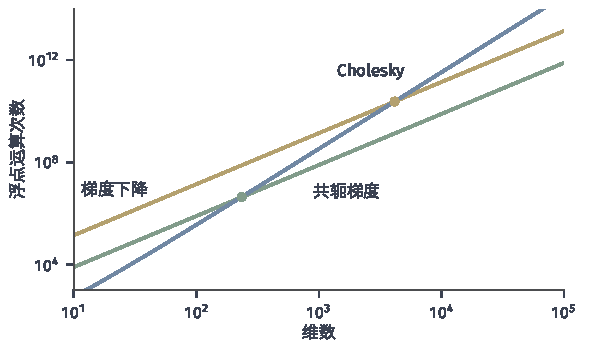
\includegraphics[width=100mm]{figures/05-optimization/02-smooth-optimization/matplotlib/smooth-work-crossover/figure.pdf}
  \caption{稠密对称正定方程的总运算量估计，$\kappa=100$，$\varepsilon=10^{-6}$。黄线为梯度下降（$691$轮），绿线为共轭梯度（$39$轮），每轮$2n^2$次运算；蓝线为Cholesky分解加回代。两个点是迭代法与分解的交叉位置，$n\approx4146$和$n\approx234$。}
  \label{fig:smooth-work-crossover}
\end{BookInlineFigure}

\paragraph{内层求解}
外层方法里嵌套内层迭代时，式~\eqref{eq:smooth-total-work}的$k^{(t)}$不能忽略。作为教学算例，假设一种用Hessian的方法外层只要$6$轮，每轮用$20$次矩阵向量积近似解方程，矩阵向量积与梯度代价相同；另一种只用梯度的方法要$60$轮。按外层轮数比较前者少$10$倍，按读取次数比较则是
\[
 6\times(1+20)=126,\qquad 60\times1=60.
\]
结论反了过来。内层容差也属于口径的一部分：内层解得越精确，外层轮数可能越少，每轮却越贵，第~\ref{chap:second-order-methods}章会讨论两者的权衡。

\paragraph{比较时要报告的内容}
把上面的要求列在一起，就是本卷后面比较算法时使用的口径，见表~\ref{tab:smooth-report}。按表中各项报告，读者才能判断两组数字是否可比。

\begin{BookInlineTable}
  \centering
  \begin{tabular}{@{}ll@{}}
    \toprule
    项目 & 需要交代的内容\\
    \midrule
    问题与起点 & 目标的结构、维数、初始点\\
    误差标准 & 目标差或驻点残差，绝对或相对容差\\
    返回规则 & 最后一轮、历史最佳或停止点\\
    外层统计 & 达到容差的轮数$T(\varepsilon)$\\
    读取统计 & 函数值、梯度、Hessian、矩阵向量积的次数\\
    被拒绝的试探 & 计入函数计算次数\\
    线性代数 & 分解、回代、内层迭代的运算量和存储\\
    结论类型 & 最坏情形的理论界，或特定问题上的实测值\\
    \bottomrule
  \end{tabular}
  \caption{比较优化算法时的报告项目。同一项目口径不同的两组结果不能直接比较。}
  \label{tab:smooth-report}
\end{BookInlineTable}

\section{本章小结}
\label{sec:smooth-summary}

本章开头问：只看得清脚下时，一步可以走多远，走完又怎样评价？回答分成三层。

光滑性给出了依据。$L$是梯度变化的限速，由它得到下降引理~\eqref{eq:smooth-descent-lemma}：一个与目标相切的二次函数从上方盖住目标。这个上界只在$L$成立的区域内有效，与凸性互不蕴含。二阶可微时最小的$L$就是Hessian谱范数的上确界。

步长规则负责检验局部预测。固定步长靠事先知道的$L$，负梯度方向上要求$\alpha<2/L$，一般方向要重新核对长度和方向导数。回溯用真实函数值检验Armijo条件，只要方向下降就有限步终止，代价是被拒绝的试探。Wolfe条件再检验落脚点的方向导数，挡住太短的步长，并保证拟牛顿更新所需的$\langle\bm{s},\bm{y}\rangle>0$；强Wolfe条件进一步限制方向导数的绝对值，供非线性共轭梯度的下降分析使用。精确线搜索只作理论对照。

比较方法要同时固定三件事：误差标准、返回的迭代点、计算量的口径。在例~\eqref{eq:smooth-running}上，同一组运行按轮数和按读取次数排出的顺序几乎相反。凸目标通常用目标差，一般非凸目标只能用驻点残差，后者只说明一阶条件满足到什么程度。式~\eqref{eq:smooth-total-work}把被拒绝的试探和内层求解都算进总计算量。

这些规则都假设了下降方向已经给定。后面几章的问题是方向从哪里来：第~\ref{chap:first-order-methods}章只用梯度和历史位移，第~\ref{chap:second-order-methods}章用Hessian，第~\ref{chap:quasi-newton}章用梯度差拼出曲率，第~\ref{chap:trust-region}章把方向和步长放在一起决定，第~\ref{chap:saddle-points}章处理非凸目标中的鞍点。各章的收敛保证需要哪些附加条件，都在本章的标准下分别说明。


\chapter{一阶方法}
\label{chap:first-order-methods}

设想站在一片山谷里，四周被雾遮住。每走到一处，只能用脚试出当地的坡度，也就是目标的函数值和梯度，看不到整个地形，也量不出地面的弯曲。这正是大规模优化最常见的处境：变量很多，Hessian算不起也存不下，一次梯度却是可以负担的。

本章全程使用同一个目标来比较各种走法：
\begin{equation}
 f(\bm{x})=\frac12\bigl(x_1^2+9x_2^2\bigr),\qquad
 \bm{x}^{(0)}=(9,1).
 \label{eq:fom-example}
\end{equation}
它的等高线是横向拉长的椭圆，最优解是原点。Hessian是$\bm{H}=\operatorname{diag}(1,9)$，所以$\mu=1$，$L=9$，$\kappa=9$。沿$x_1$方向地面平缓，沿$x_2$方向地面陡峭，这种“一个方向平、一个方向陡”的山谷称为病态的目标。

最朴素的走法是每步顺着最陡的方向下山。第~\ref{sec:fom-gradient-descent}节会看到，它在这个山谷里左右折返，大部分力气消耗在陡峭方向上。那么，能不能利用走过的路？第~\ref{sec:fom-momentum}节把上一步的位移加进当前更新，并比较梯度取在当前点和取在试探点这两种做法。第~\ref{sec:fom-ncg}节换一种用历史的方式：保留上一轮的搜索方向，与新梯度组合，再用线搜索决定走多远。

几种方法花费的计算不同，得到的保证也不同。有的保证只对二次目标成立，有的要求凸，有的只能说梯度变小。第~\ref{sec:fom-cost}节把它们放在同一把尺子下比较，并说明为什么迭代次数少不等于总计算少。

\section{梯度下降}
\label{sec:fom-gradient-descent}

只知道当前点的函数值和梯度，下一步应该朝哪里走、走多远？本节回答这个问题，并分三种情形说明这样走能得到什么：一般非凸、凸、强凸。三种情形的结论强弱不同，度量误差的尺子也不同。

\paragraph{主要思想}
先看方向。在$\bm{x}$附近，目标由一阶Taylor展开近似：
\[
 f(\bm{x}+\bm{d})\approx f(\bm{x})+\nabla f(\bm{x})^\top\bm{d}.
\]
在固定长度的$\bm{d}$中，要让$\nabla f(\bm{x})^\top\bm{d}$最小。由Cauchy--Schwarz不等式，
\[
 \nabla f(\bm{x})^\top\bm{d}\geq-\lVert\nabla f(\bm{x})\rVert_2\lVert\bm{d}\rVert_2,
\]
等号当且仅当$\bm{d}$与$-\nabla f(\bm{x})$同向时成立。所以局部最陡的下降方向是负梯度方向。

线性模型只给方向，不给距离：沿负梯度走得越远，线性模型的值越低，没有尽头。真实的地面会弯曲，线性预测走远了就不可信。需要一个量来说明“能信多远”。

这个量就是第~\ref{chap:smooth-foundations}章的光滑常数$L$，它要求梯度满足Lipschitz条件：
\[
 \lVert\nabla f(\bm{x})-\nabla f(\bm{y})\rVert_2\leq L\lVert\bm{x}-\bm{y}\rVert_2.
\]

在这个条件下，下降引理给出处处成立的二次上界：
\begin{equation}
 f(\bm{y})\leq f(\bm{x})+\nabla f(\bm{x})^\top(\bm{y}-\bm{x})+\frac{L}{2}\lVert\bm{y}-\bm{x}\rVert_2^2.
 \label{eq:fom-descent-lemma}
\end{equation}
二阶可微时，$\nabla^2f\preceq L\bm{I}$且$\nabla^2f\succeq-L\bm{I}$就保证了这一点。可以把右端想成扣在地面上的一只碗：它在$\bm{x}$处贴住地面，其余地方都不低于地面。

既然地面不高于这只碗，就走到碗底。对$\bm{y}$求右端的最小点，令导数为零，得到$\bm{y}=\bm{x}-\nabla f(\bm{x})/L$。图~\ref{fig:fom-upper-bound}画的是一元的情形：绿色的碗底对应的横坐标就是新点，碗底的高度保证了至少下降多少。

\begin{BookInlineFigure}
  \centering
  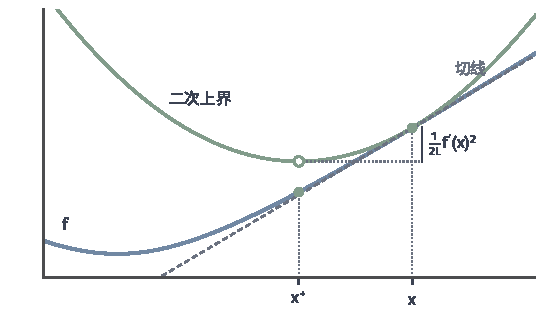
\includegraphics[width=92mm]{figures/05-optimization/02-smooth-optimization/matplotlib/fom-upper-bound/figure.pdf}
  \caption{二次上界决定一步走多远。蓝色曲线是$f(x)=\sqrt{1+x^2}$，它的二阶导数不超过$1$，取$L=1$。虚线是$x=2.4$处的切线，绿色抛物线是式~\eqref{eq:fom-descent-lemma}的上界。空心点是上界的最低点，其横坐标$x^{+}$就是新点，实心点是真实的函数值，它不高于空心点。竖线段是保证的下降量。}
  \label{fig:fom-upper-bound}
\end{BookInlineFigure}

把步长放宽为任意的$\alpha>0$，就得到\term{梯度下降法}（gradient descent method）：
\begin{equation}
 \bm{x}^{(t+1)}=\bm{x}^{(t)}-\alpha^{(t)}\bm{g}^{(t)},\qquad \bm{g}^{(t)}=\nabla f(\bm{x}^{(t)}).
 \label{eq:fom-gd}
\end{equation}
把$\bm{y}=\bm{x}^{(t+1)}$代入式~\eqref{eq:fom-descent-lemma}，一阶项是$-\alpha\lVert\bm{g}^{(t)}\rVert_2^2$，二次项是$\tfrac{L}{2}\alpha^2\lVert\bm{g}^{(t)}\rVert_2^2$，合起来得到单步下降估计：
\begin{equation}
 f(\bm{x}^{(t+1)})\leq f(\bm{x}^{(t)})-\alpha\Bigl(1-\frac{L\alpha}{2}\Bigr)\lVert\bm{g}^{(t)}\rVert_2^2.
 \label{eq:fom-gd-decrease}
\end{equation}
只要$0<\alpha<2/L$，括号就是正的，函数值严格下降。关于$\alpha$求最大的下降量，得到$\alpha=1/L$，此时每步至少下降$\lVert\bm{g}^{(t)}\rVert_2^2/(2L)$。

步长的来源有三种，都沿用第~\ref{chap:smooth-foundations}章的规则。已知$L$时取固定步长；不知道$L$时用回溯，从一个试探值开始不断缩短，直到满足Armijo条件
\begin{equation}
 f(\bm{x}+\alpha\bm{d})\leq f(\bm{x})+c_1\alpha\nabla f(\bm{x})^\top\bm{d},\qquad 0<c_1<1;
 \label{eq:fom-armijo}
\end{equation}
二次目标上还可以精确求沿线最小点。负梯度方向的精确步长是
\[
 \alpha=\frac{\bm{g}^\top\bm{g}}{\bm{g}^\top\bm{H}\bm{g}},
\]
这时的方法称为最速下降法（steepest descent）。

\needspace{6\baselineskip}
\paragraph{变量}
\begin{itemize}
 \item $\bm{x}^{(t)}\in\mathbb{R}^n$：当前点，在原处更新。
 \item $\bm{g}^{(t)}\in\mathbb{R}^n$：当前点的梯度，每轮读取一次。
 \item $\alpha>0$：步长，这里固定；用线搜索时每轮重新确定。
 \item $\varepsilon>0$，$T$：梯度大小的容差与最大步数。
\end{itemize}

\paragraph{初始化}
选定起点$\bm{x}^{(0)}$、步长、容差，令$t=0$。例中用式~\eqref{eq:fom-example}的起点，并取$\alpha=1/5$（下文说明这个值从哪里来），容差$\varepsilon=10^{-3}$。初始值是
\[
 \bm{x}^{(0)}=(9,1),\qquad f(\bm{x}^{(0)})=45.
\]

\needspace{6\baselineskip}
\paragraph{每轮更新}
在第$t$轮：
\begin{enumerate}
 \item \textbf{读取梯度。}计算$\bm{g}^{(t)}=\nabla f(\bm{x}^{(t)})$。例中$\nabla f(\bm{x})=(x_1,9x_2)$，第一轮
 \[
  \bm{g}^{(0)}=(9,9).
 \]
 \item \textbf{检查停止。}若$\lVert\bm{g}^{(t)}\rVert_2\leq\varepsilon$或$t=T$，输出$\bm{x}^{(t)}$并结束。例中第一轮$\lVert\bm{g}^{(0)}\rVert_2=9\sqrt2\approx12.73$，继续。
 \item \textbf{更新。}按式~\eqref{eq:fom-gd}计算新点，令$t\leftarrow t+1$。例中第一轮
 \[
  \bm{x}^{(1)}=(9,1)-\tfrac15(9,9)=(7.2,-0.8),\qquad f(\bm{x}^{(1)})=28.8.
 \]

 例中第二轮$\bm{g}^{(1)}=(7.2,-7.2)$，于是
 \[
  \bm{x}^{(2)}=(7.2,-0.8)-\tfrac15(7.2,-7.2)=(5.76,0.64),
 \]
 目标值$f(\bm{x}^{(2)})=18.432$。

 例中第三轮$\bm{g}^{(2)}=(5.76,5.76)$，于是
 \[
  \bm{x}^{(3)}=(5.76,0.64)-\tfrac15(5.76,5.76)=(4.608,-0.512),
 \]
 目标值$f(\bm{x}^{(3)})=11.79648$。
\end{enumerate}

规律已经显出来了：两个坐标分别乘以$1-\alpha\lambda$，第一个因子是$1-\tfrac15=0.8$，第二个因子是$1-\tfrac95=-0.8$。因此
\[
 \bm{x}^{(t)}=0.8^t\bigl(9,(-1)^t\bigr),\qquad f(\bm{x}^{(t)})=45\cdot0.64^t.
\]

梯度大小是$\lVert\bm{g}^{(t)}\rVert_2=0.8^t\cdot9\sqrt2$，它不超过$10^{-3}$要求$t\geq43$。最终得到
\[
 \bm{x}^{(43)}\approx(6.13\times10^{-4},\,-6.81\times10^{-5}).
\]
这个起点是特意选的：沿$\bm{d}=-\bm{g}$的精确步长恰好处处等于$1/5$，所以这串点也是最速下降的结果。

\paragraph{步长与收缩因子}
为什么取$1/5$，而不是上界推出的$1/L=1/9$？这要看二次目标上一步到底做了什么。设
\[
 f(\bm{x})=\frac12(\bm{x}-\bm{x}^\star)^\top\bm{H}(\bm{x}-\bm{x}^\star)+f^\star,
\]
其中$\bm{H}$对称正定，特征值都落在$[\mu,L]$内。记$\bm{e}^{(t)}=\bm{x}^{(t)}-\bm{x}^\star$，由$\bm{g}^{(t)}=\bm{H}\bm{e}^{(t)}$得
\[
 \bm{e}^{(t+1)}=(\bm{I}-\alpha\bm{H})\bm{e}^{(t)}.
\]

用$\bm{H}$的标准正交特征向量作坐标，矩阵变成对角形，每个特征方向各自演化。特征值为$\lambda$的分量每步乘以同一个数：
\begin{equation}
 e_\lambda^{(t+1)}=(1-\alpha\lambda)\,e_\lambda^{(t)}.
 \label{eq:fom-gd-factor}
\end{equation}
特征分解的做法可参考\BookChapterRef{chap:eigen-spectral-decomposition}{卷二第6章“谱分解”}。

步长是所有方向共用的一个数，而不同方向希望的步长不同：$\lambda$方向最想要$\alpha=1/\lambda$，一步到位。图~\ref{fig:fom-step-factor}把例中两个方向的因子画在一起。陡峭方向的折线下降得快，在$\alpha=1/9$处触底，随后反弹；平坦方向的线缓慢下降。整体的进度取决于两条线中较高的那条。

\begin{BookInlineFigure}
  \centering
  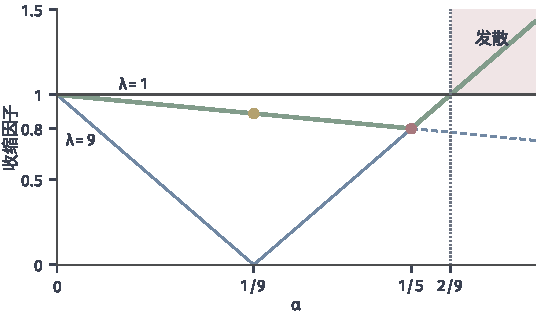
\includegraphics[width=92mm]{figures/05-optimization/02-smooth-optimization/matplotlib/fom-step-factor/figure.pdf}
  \caption{贯穿例上两个特征方向的收缩因子$\lvert1-\alpha\lambda\rvert$。蓝色实线对应陡峭方向$\lambda=9$，蓝色虚线对应平坦方向$\lambda=1$，绿色粗线是两者的较大值。黄点是$\alpha=1/L=1/9$，红点是使较大值最小的$\alpha=2/(L+\mu)=1/5$，此时因子等于$0.8$。红底区域$\alpha>2/9$中因子超过$1$，迭代发散。}
  \label{fig:fom-step-factor}
\end{BookInlineFigure}

要让最慢的方向尽量快，就让两条线相交。这件事可以写成一条定理。

\begin{theorem}[二次目标上的最佳固定步长]
\label{thm:fom-gd-quadratic}
设$\bm{H}$对称正定，特征值落在$[\mu,L]$内，且$\mu$和$L$都是特征值。固定步长的梯度下降收敛到$\bm{x}^\star$（对任意起点）当且仅当$0<\alpha<2/L$。取$\alpha=2/(L+\mu)$时，最大收缩因子最小，并且
\begin{equation}
 \lVert\bm{x}^{(t)}-\bm{x}^\star\rVert_2\leq\Bigl(\frac{\kappa-1}{\kappa+1}\Bigr)^t\lVert\bm{x}^{(0)}-\bm{x}^\star\rVert_2.
 \label{eq:fom-gd-quadratic-rate}
\end{equation}
\end{theorem}

\begin{proof}
由式~\eqref{eq:fom-gd-factor}，第$t$步的$\lambda$分量等于$(1-\alpha\lambda)^t$乘以初值。任意起点都收敛，当且仅当对每个特征值都有$\lvert1-\alpha\lambda\rvert<1$，即$0<\alpha\lambda<2$。这在$\lambda=L$时最严格，所以条件是$0<\alpha<2/L$。

函数$\lvert1-\alpha\lambda\rvert$关于$\lambda$是凸的，在$[\mu,L]$上的最大值在端点取得，所以最大因子是
\[
 \rho(\alpha)=\max\{\lvert1-\alpha\mu\rvert,\lvert1-\alpha L\rvert\}.
\]

随着$\alpha$增大，$1-\alpha\mu$减小，$\alpha L-1$增大。两者相等时最大值最小，这时$1-\alpha\mu=\alpha L-1$，解得
\[
 \alpha=\frac{2}{L+\mu},\qquad \rho=1-\frac{2\mu}{L+\mu}=\frac{\kappa-1}{\kappa+1}.
\]

最后，标准正交变换保持欧氏长度，各分量的平方和至多缩小$\rho^2$倍，即得结论。
\end{proof}

例中$\kappa=9$，$\rho=8/10=0.8$，正是上面算出的因子。起点$(9,1)$使两个方向同时达到这一因子，所以界~\eqref{eq:fom-gd-quadratic-rate}在这个例子上取等号。

图~\ref{fig:fom-gd-paths}把步长的影响画在等高线上。$\alpha=1/9$时第一步就消掉了$x_2$，随后沿谷底以因子$8/9$慢慢前进，路径光滑但慢；$\alpha=1/5$时路径左右折返，前进因子却是$0.8$；$\alpha=0.23$超过了$2/9$，$x_2$每步乘以$-1.07$，折返幅度越来越大。

\begin{BookInlineFigure}
  \centering
  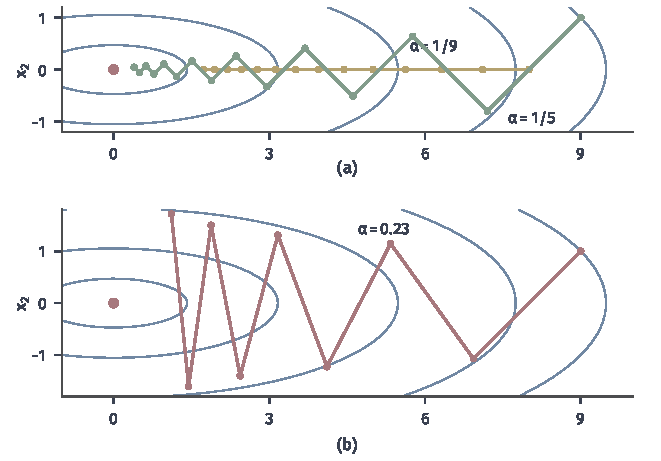
\includegraphics[width=112mm]{figures/05-optimization/02-smooth-optimization/matplotlib/fom-gd-paths/figure.pdf}
  \caption{贯穿例上不同固定步长的路径，蓝色椭圆是等高线，红点是最优解。(a)黄色路径$\alpha=1/9$，绿色路径$\alpha=1/5$，各走$14$步。(b)红色路径$\alpha=0.23>2/L$，走$8$步，$x_1$在收缩，$x_2$的振幅却在放大。}
  \label{fig:fom-gd-paths}
\end{BookInlineFigure}

于是$\alpha=1/L$与$\alpha=2/(L+\mu)$回答的是两个不同的问题。前者由上界推出，只用$L$，保证函数值每步下降，下面的定理都以它为基础；后者要同时知道$\mu$和$L$，它在二次目标上收缩最快，函数值也下降，但路径来回摆动。

\paragraph{一般非凸情形：梯度残差}
下面离开二次目标。先看最弱的假设：$f$可以非凸，只要求梯度Lipschitz，并且有下界。这时目标差和解距离都无从谈起，因为可能有许多局部的谷底，能评价的只有梯度的大小。

\begin{theorem}[非凸情形的梯度下降]
\label{thm:fom-gd-nonconvex}
设$f$的梯度$L$-Lipschitz连续，$f_{\inf}=\inf f>-\infty$。取固定步长$\alpha=1/L$，则对任意$T\geq1$，
\begin{equation}
 \min_{0\leq t<T}\lVert\bm{g}^{(t)}\rVert_2^2\leq\frac{2L\bigl(f(\bm{x}^{(0)})-f_{\inf}\bigr)}{T},
 \label{eq:fom-gd-nonconvex}
\end{equation}
并且$\lVert\bm{g}^{(t)}\rVert_2\to0$，$\{\bm{x}^{(t)}\}$的每个极限点都是驻点。
\end{theorem}

\begin{proof}
由式~\eqref{eq:fom-gd-decrease}，取$\alpha=1/L$时每步满足
\[
 \frac{1}{2L}\lVert\bm{g}^{(t)}\rVert_2^2\leq f(\bm{x}^{(t)})-f(\bm{x}^{(t+1)}).
\]

对$t=0,\ldots,T-1$求和，右端裂项，再用$f(\bm{x}^{(T)})\geq f_{\inf}$，得到
\[
 \frac{1}{2L}\sum_{t=0}^{T-1}\lVert\bm{g}^{(t)}\rVert_2^2\leq f(\bm{x}^{(0)})-f_{\inf}.
\]

$T$项的最小值不超过平均值，这就是式~\eqref{eq:fom-gd-nonconvex}。令$T\to\infty$，上式说明级数$\sum\lVert\bm{g}^{(t)}\rVert_2^2$收敛，所以通项趋于零。$\nabla f$连续，极限点处的梯度等于梯度序列的极限，也就是零。
\end{proof}

定理说的是“某一步的梯度够小”，并没有说最后一步最小，所以输出时要记住梯度最小的那个迭代点。换成任意$\alpha\in(0,2/L)$，只需把$1/(2L)$换成$\alpha(1-L\alpha/2)$。

用回溯时结论同样成立，只差常数。由式~\eqref{eq:fom-gd-decrease}，凡是$\alpha\leq2(1-c_1)/L$的步长都满足Armijo条件。所以若初始试探值为$\alpha_0$、每次缩短到$\rho$倍，接受的步长不低于$\min\{\alpha_0,2\rho(1-c_1)/L\}$，每步下降量有与上面同样形式的下界。

驻点不等于极小点。图~\ref{fig:fom-nonconvex}取非凸函数$f(\bm{x})=-\cos x_1+\tfrac92x_2^2$，它的Hessian是$\operatorname{diag}(\cos x_1,9)$，所以$L=9$，下确界是$-1$。从$(\pi,1)$出发的路径停在鞍点$(\pi,0)$，梯度为零，定理完全满足，点却不是局部最优解。稍稍偏开，从$(3,1)$出发，路径在鞍点附近徘徊一阵，再滑向真正的谷底。

\begin{BookInlineFigure}
  \centering
  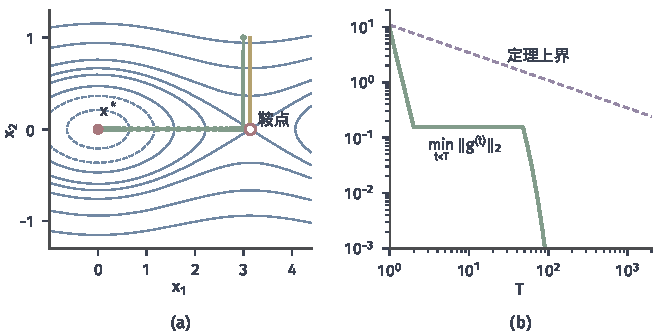
\includegraphics[width=112mm]{figures/05-optimization/02-smooth-optimization/matplotlib/fom-nonconvex/figure.pdf}
  \caption{非凸目标$f(\bm{x})=-\cos x_1+\tfrac92x_2^2$上取$\alpha=1/9$的梯度下降。(a)等高线与两条路径：黄色从$(\pi,1)$出发，终止于鞍点（红色空心点）；绿色从$(3,1)$出发，到达极小点（红点）。(b)绿色路径的$\min_{t<T}\lVert\bm{g}^{(t)}\rVert_2$（绿线），紫色虚线是式~\eqref{eq:fom-gd-nonconvex}的上界开方。中段的平台对应在鞍点附近的徘徊。}
  \label{fig:fom-nonconvex}
\end{BookInlineFigure}

\paragraph{凸情形：目标差}
加上凸性后，局部的谷底就是全局的谷底，可以用目标差来衡量。关键的新工具是：切平面从下方托住目标，用它比较当前点和最优解。

\begin{theorem}[凸情形的梯度下降]
\label{thm:fom-gd-convex}
设$f$凸，梯度$L$-Lipschitz连续，且存在最优解$\bm{x}^\star$。取$\alpha=1/L$，则对任意$T\geq1$，
\begin{equation}
 f(\bm{x}^{(T)})-f^\star\leq\frac{L\lVert\bm{x}^{(0)}-\bm{x}^\star\rVert_2^2}{2T}.
 \label{eq:fom-gd-convex}
\end{equation}
\end{theorem}

\begin{proof}
记$\bm{x}=\bm{x}^{(t)}$，$\bm{x}^+=\bm{x}^{(t+1)}$，$\bm{g}=\bm{g}^{(t)}$。由凸性，切平面在$\bm{x}^\star$处不高于目标：
\[
 f^\star\geq f(\bm{x})+\bm{g}^\top(\bm{x}^\star-\bm{x}).
\]

由式~\eqref{eq:fom-gd-decrease}，$\alpha=1/L$时单步下降至少为$\lVert\bm{g}\rVert_2^2/(2L)$。把上式代入，得到
\[
 f(\bm{x}^+)-f^\star\leq\bm{g}^\top(\bm{x}-\bm{x}^\star)-\frac{1}{2L}\lVert\bm{g}\rVert_2^2.
\]

把$\bm{x}^+=\bm{x}-\bm{g}/L$代入距离的平方，展开得
\[
 \lVert\bm{x}^+-\bm{x}^\star\rVert_2^2
 =\lVert\bm{x}-\bm{x}^\star\rVert_2^2-\frac2L\bm{g}^\top(\bm{x}-\bm{x}^\star)+\frac{1}{L^2}\lVert\bm{g}\rVert_2^2.
\]

两式比较，前一式的右端恰好等于距离平方之差的$L/2$倍：
\[
 f(\bm{x}^{(t+1)})-f^\star\leq\frac L2\Bigl(\lVert\bm{x}^{(t)}-\bm{x}^\star\rVert_2^2-\lVert\bm{x}^{(t+1)}-\bm{x}^\star\rVert_2^2\Bigr).
\]

对$t=0,\ldots,T-1$求和，右端裂项，丢掉末项，得到
\[
 \sum_{t=1}^{T}\bigl(f(\bm{x}^{(t)})-f^\star\bigr)\leq\frac L2\lVert\bm{x}^{(0)}-\bm{x}^\star\rVert_2^2.
\]

函数值逐步下降，所以最后一项是$T$项中最小的，不超过平均值，即得式~\eqref{eq:fom-gd-convex}。
\end{proof}

上面证明还顺带说明，到最优解的距离每步不增。

$1/T$这个阶对梯度下降不能改进。取$f(\bm{x})=\tfrac12(Lx_1^2+\lambda x_2^2)$，$0<\lambda\leq L$，起点的第一坐标为$0$，第二坐标为$x_0$。$\alpha=1/L$时目标差是$\tfrac12\lambda(1-\lambda/L)^{2T}x_0^2$。对每个给定的$T$，取$\lambda=L/(2T)$，因子$(1-1/(2T))^{2T}$接近$\mathrm{e}^{-1}$，于是目标差约为
\[
 \frac{Lx_0^2}{4\mathrm{e}\,T}.
\]
也就是说，曲率总可以小到让梯度下降在这$T$步内几乎察觉不到。这个例子的$\lambda$随$T$变化，它说明上界在整个函数类上的阶不能改进，并不是说某个固定的二次目标只有$1/T$的速度。

\paragraph{强凸情形：线性收敛}
再加上强凸，第~\ref{chap:optimization}章的结论告诉我们解存在且唯一。这时切平面之上还多出一个二次项：
\begin{equation}
 f(\bm{y})\geq f(\bm{x})+\nabla f(\bm{x})^\top(\bm{y}-\bm{x})+\frac\mu2\lVert\bm{y}-\bm{x}\rVert_2^2.
 \label{eq:fom-strong-convexity}
\end{equation}
这是一只从下方托住地面的碗，与式~\eqref{eq:fom-descent-lemma}从上方扣住地面的碗相对。上下两只碗夹住地形，每步的进度就能与当前的误差比较。

\begin{theorem}[强凸情形的梯度下降]
\label{thm:fom-gd-strong}
设$f$的梯度$L$-Lipschitz连续且满足式~\eqref{eq:fom-strong-convexity}，$\mu>0$，$\kappa=L/\mu$。取$\alpha=1/L$，则
\begin{equation}
 \begin{aligned}
 f(\bm{x}^{(T)})-f^\star&\leq\Bigl(1-\frac1\kappa\Bigr)^T\bigl(f(\bm{x}^{(0)})-f^\star\bigr),\\
 \lVert\bm{x}^{(T)}-\bm{x}^\star\rVert_2^2&\leq\Bigl(1-\frac1\kappa\Bigr)^T\lVert\bm{x}^{(0)}-\bm{x}^\star\rVert_2^2.
 \end{aligned}
 \label{eq:fom-gd-strong}
\end{equation}
\end{theorem}

\begin{proof}
先证梯度能控制目标差。在式~\eqref{eq:fom-strong-convexity}中对$\bm{y}$取右端的最小值，最小点是$\bm{y}=\bm{x}-\nabla f(\bm{x})/\mu$，于是
\[
 f^\star\geq f(\bm{x})-\frac{1}{2\mu}\lVert\nabla f(\bm{x})\rVert_2^2,
 \qquad\text{即}\qquad
 \lVert\nabla f(\bm{x})\rVert_2^2\geq2\mu\bigl(f(\bm{x})-f^\star\bigr).
\]

代入式~\eqref{eq:fom-gd-decrease}（$\alpha=1/L$），两边减去$f^\star$，得到
\[
 f(\bm{x}^+)-f^\star\leq\Bigl(1-\frac\mu L\Bigr)\bigl(f(\bm{x})-f^\star\bigr).
\]
迭代$T$次即得第一式。

再证距离。在式~\eqref{eq:fom-strong-convexity}中取$\bm{y}=\bm{x}^\star$，整理得
\[
 \bm{g}^\top(\bm{x}-\bm{x}^\star)\geq f(\bm{x})-f^\star+\frac\mu2\lVert\bm{x}-\bm{x}^\star\rVert_2^2.
\]

另由$f^\star\leq f(\bm{x}^+)$和单步下降，得到
\[
 \lVert\bm{g}\rVert_2^2\leq2L\bigl(f(\bm{x})-f^\star\bigr).
\]

把这两式代入距离平方的展开式：
\[
 \begin{aligned}
 \lVert\bm{x}^+-\bm{x}^\star\rVert_2^2
 &=\lVert\bm{x}-\bm{x}^\star\rVert_2^2-\frac2L\bm{g}^\top(\bm{x}-\bm{x}^\star)+\frac{1}{L^2}\lVert\bm{g}\rVert_2^2\\
 &\leq\Bigl(1-\frac\mu L\Bigr)\lVert\bm{x}-\bm{x}^\star\rVert_2^2-\frac2L\bigl(f(\bm{x})-f^\star\bigr)+\frac2L\bigl(f(\bm{x})-f^\star\bigr).
 \end{aligned}
\]
后两项抵消，迭代$T$次即得第二式。
\end{proof}

用贯穿例核对。$\alpha=1/9$时$\bm{x}^{(1)}=(8,0)$，此后第一坐标每步乘以$8/9$，所以
\[
 f(\bm{x}^{(T)})=32\Bigl(\frac{64}{81}\Bigr)^{T-1},\qquad T\geq1.
\]
定理的上界是$45\cdot(8/9)^T$，$T=1$时是$40$，大于真实值$32$。图~\ref{fig:fom-gd-rates}(a)显示，上界比真实的衰减慢：定理覆盖所有满足条件的函数，这个二次例子并不是最坏的。

\paragraph{条件数怎样影响进展}
三条定理合起来回答了“要多少步”。目标差达到$\varepsilon$所需的步数，凸时约为$LR^2/(2\varepsilon)$，其中$R=\lVert\bm{x}^{(0)}-\bm{x}^\star\rVert_2$；强凸时由$(1-1/\kappa)^T\leq\mathrm{e}^{-T/\kappa}$得到
\[
 T\geq\kappa\ln\frac{f(\bm{x}^{(0)})-f^\star}{\varepsilon}.
\]

所需步数与$\kappa$成正比。把山谷的纵横比拉大十倍，步数也大约变成十倍。图~\ref{fig:fom-gd-rates}(b)对$\operatorname{diag}(1,\kappa)$实测目标差降到初值$10^{-6}$的步数，它紧贴直线$\tfrac\kappa4\ln(1/\varepsilon)$。这里$\tfrac14$来自最佳步长：因子$(\kappa-1)/(\kappa+1)$约为$1-2/\kappa$，目标差的因子是其平方。

\begin{BookInlineFigure}
  \centering
  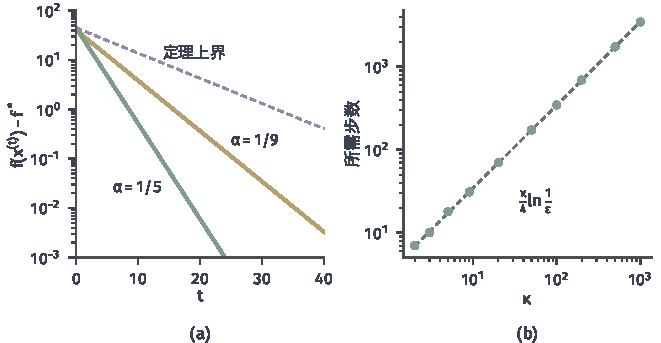
\includegraphics[width=112mm]{figures/05-optimization/02-smooth-optimization/matplotlib/fom-gd-rates/figure.pdf}
  \caption{收敛速度与条件数。(a)贯穿例的目标差：黄线$\alpha=1/9$，绿线$\alpha=1/5$，紫色虚线是$\alpha=1/L$时式~\eqref{eq:fom-gd-strong}的上界$45(8/9)^t$。(b)目标$\tfrac12(x_1^2+\kappa x_2^2)$，起点$(\kappa,1)$，步长$2/(1+\kappa)$，绿点是目标差降到初值$10^{-6}$倍的实测步数，虚线为$\tfrac\kappa4\ln(1/\varepsilon)$，$\varepsilon=10^{-6}$。}
  \label{fig:fom-gd-rates}
\end{BookInlineFigure}

原因已经在式~\eqref{eq:fom-gd-factor}中：步长被陡峭方向限制在$2/L$以内，平坦方向每步只能收缩$\mu/L$量级的比例。下面的表格汇总三种情形。

\begin{BookInlineTable}
  \centering
  \caption{梯度下降$\alpha=1/L$的保证，$\Delta=f(\bm{x}^{(0)})-f_{\inf}$，$R=\lVert\bm{x}^{(0)}-\bm{x}^\star\rVert_2$。}
  \label{tab:fom-gd-summary}
  \begin{tabular}{llll}
   \toprule
   假设 & 度量 & 上界 & 达到$\varepsilon$的步数\\
   \midrule
   非凸，有下界 & $\min_t\lVert\bm{g}^{(t)}\rVert_2^2$ & $2L\Delta/T$ & $2L\Delta/\varepsilon$\\
   凸 & $f(\bm{x}^{(T)})-f^\star$ & $LR^2/(2T)$ & $LR^2/(2\varepsilon)$\\
   强凸 & $f(\bm{x}^{(T)})-f^\star$ & $(1-1/\kappa)^T\Delta$ & $\kappa\ln(\Delta/\varepsilon)$\\
   \bottomrule
  \end{tabular}
\end{BookInlineTable}

表中第一行的$\varepsilon$是梯度平方的容差，所以换成梯度大小达到$\varepsilon$时，步数是$2L\Delta/\varepsilon^2$。三行的度量不同，步数不能直接相比。

\section{动量与加速}
\label{sec:fom-momentum}

上一节的结论是：病态目标上梯度下降的步数与$\kappa$成正比。不增加每步的梯度读取次数，只多用一点历史信息，能不能把这个依赖关系变小？

先看贯穿例上折返时发生了什么。图~\ref{fig:fom-zigzag}(a)把$\alpha=1/5$的每步位移分解到两个坐标。平坦方向$x_1$上，每一步的位移都向负方向，符号一致；陡峭方向$x_2$上，位移的符号每步翻转，走过去又走回来，大部分抵消。

\begin{BookInlineFigure}
  \centering
  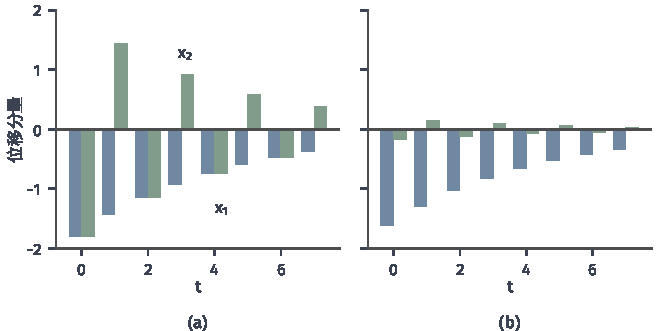
\includegraphics[width=112mm]{figures/05-optimization/02-smooth-optimization/matplotlib/fom-zigzag/figure.pdf}
  \caption{贯穿例上$\alpha=1/5$的梯度下降的位移。蓝色条是平坦方向$x_1$的分量，绿色条是陡峭方向$x_2$的分量。(a)每一步的位移$\bm{x}^{(t+1)}-\bm{x}^{(t)}$，绿色条的符号逐步交替。(b)相邻两步位移的平均，绿色条几乎消失，蓝色条保持不变的符号与相近的大小。}
  \label{fig:fom-zigzag}
\end{BookInlineFigure}

图~\ref{fig:fom-zigzag}(b)把相邻两步取平均：振荡方向互相抵消，一致方向得以保留。这就是用历史信息的线索：过去的位移本身携带了“哪些方向一直在走、哪些方向在来回”的信息，而这一信息不用额外计算梯度。

把上一步的位移乘一个系数加进当前更新，这个附加量称为\term{动量}（momentum）。下面两个方法都用动量，差别在梯度取在什么地方：重球法取在当前点，Nesterov方法取在沿动量向前试探的点。

\subsection{Polyak重球法}
\label{sec:fom-heavy-ball}

\paragraph{主要思想}
想象一个有质量的球在山谷中滚动，并受到摩擦。球的速度不会突然改变：沿谷底方向的重力持续推动，它越滚越快；沿谷壁方向的重力来回变号，速度被平均掉了。这就是想要的效果。

类比可以写成方程。位置$\bm{x}(\tau)$满足
\[
 \ddot{\bm{x}}+a\dot{\bm{x}}+\nabla f(\bm{x})=\bm{0},
\]
其中$a>0$是摩擦系数。用步长$h$的差分代替导数：
\[
 \ddot{\bm{x}}\approx\frac{\bm{x}^{(t+1)}-2\bm{x}^{(t)}+\bm{x}^{(t-1)}}{h^2},\qquad
 \dot{\bm{x}}\approx\frac{\bm{x}^{(t)}-\bm{x}^{(t-1)}}{h}.
\]

代入方程并整理，得到\term{重球法}（heavy ball method）\scite{polyak1964heavyball}：
\begin{equation}
 \bm{x}^{(t+1)}=\bm{x}^{(t)}-\alpha\bm{g}^{(t)}+\beta\bigl(\bm{x}^{(t)}-\bm{x}^{(t-1)}\bigr),
 \label{eq:fom-hb}
\end{equation}
其中$\alpha=h^2$，$\beta=1-ah$。摩擦越小，$\beta$越接近$1$，历史保留得越多。类比只解释了公式的样子，它并不提供收敛保证：离散的步子可以跨过谷底，下面会看到这确实造成困难。

$\alpha$和$\beta$怎样选？在正定二次目标上可以精确分析。与梯度下降一样，取$\bm{H}$的特征方向作坐标，由式~\eqref{eq:fom-hb}，特征值$\lambda$对应的误差分量满足二阶递推
\begin{equation}
 e_\lambda^{(t+1)}=(1+\beta-\alpha\lambda)e_\lambda^{(t)}-\beta e_\lambda^{(t-1)}.
 \label{eq:fom-hb-scalar}
\end{equation}

二阶线性递推的行为由特征方程的两个根决定：
\begin{equation}
 r^2-(1+\beta-\alpha\lambda)r+\beta=0.
 \label{eq:fom-hb-char}
\end{equation}
两根之积是$\beta$。判别式小于零时两根共轭，模相等，所以模都等于$\sqrt\beta$，\emph{与$\lambda$无关}。这是重球法最关键的现象：梯度下降的因子$1-\alpha\lambda$随方向变化，动量却可以把一段特征值的收缩速度拉平。

判别式小于等于零，就是$\lvert1+\beta-\alpha\lambda\rvert\leq2\sqrt\beta$。把它拆成上下两个不等式，并用$1+\beta\mp2\sqrt\beta=(1\mp\sqrt\beta)^2$，得到
\begin{equation}
 (1-\sqrt\beta)^2\leq\alpha\lambda\leq(1+\sqrt\beta)^2.
 \label{eq:fom-hb-complex}
\end{equation}
落在这个区间内的$\lambda$，收缩因子都是$\sqrt\beta$；落在区间外时两根是实数，积为$\beta$，其中一个的绝对值大于$\sqrt\beta$，收缩变慢。

于是设计问题变得清楚：让$[\alpha\mu,\alpha L]$全部落入区间~\eqref{eq:fom-hb-complex}，同时让$\sqrt\beta$尽量小。$\beta$越小区间越窄，所以最优时区间的两端恰好卡住，
\[
 (1-\sqrt\beta)^2=\alpha\mu,\qquad(1+\sqrt\beta)^2=\alpha L.
\]

两式开方后相除，得到$\sqrt\kappa=(1+\sqrt\beta)/(1-\sqrt\beta)$，解出$\sqrt\beta$；两式开方后相加，得到$\sqrt{\alpha L}+\sqrt{\alpha\mu}=2$，解出$\alpha$。结果是
\begin{equation}
 \alpha=\frac{4}{(\sqrt L+\sqrt\mu)^2},\qquad
 \beta=\Bigl(\frac{\sqrt\kappa-1}{\sqrt\kappa+1}\Bigr)^2.
 \label{eq:fom-hb-params}
\end{equation}
收缩因子$\sqrt\beta=(\sqrt\kappa-1)/(\sqrt\kappa+1)$的形式与梯度下降相同，只是$\kappa$换成了$\sqrt\kappa$。

例中$L=9$，$\mu=1$，$\sqrt\kappa=3$，所以
\[
 \alpha=\frac{4}{(3+1)^2}=\frac14,\qquad\beta=\Bigl(\frac24\Bigr)^2=\frac14,\qquad\sqrt\beta=\frac12.
\]

图~\ref{fig:fom-hb-roots}(a)画出$\lambda$从$1$走到$9$时根的运动。$\lambda=1$时是实轴上的二重根$\tfrac12$，随着$\lambda$增大，两根沿半径$\tfrac12$的圆分开，在$\lambda=5$时到达$\pm\tfrac12\mathrm{i}$，再在$\lambda=9$时汇合于$-\tfrac12$。梯度下降的单根则在实轴上从$0.8$移动到$-0.8$。图~\ref{fig:fom-hb-roots}(b)把模按$\lambda$展开：梯度下降是V形，重球法是平底。

\begin{BookInlineFigure}
  \centering
  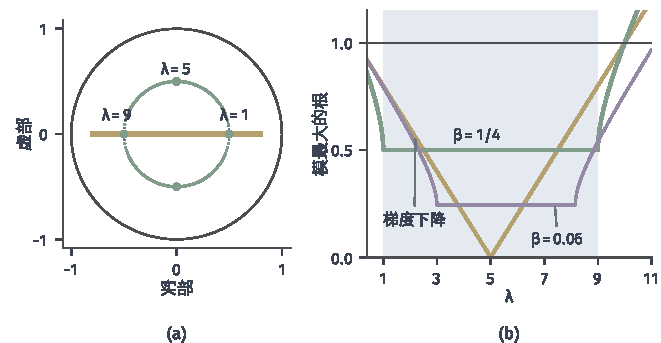
\includegraphics[width=112mm]{figures/05-optimization/02-smooth-optimization/matplotlib/fom-hb-roots/figure.pdf}
  \caption{重球法的特征根。(a)$\alpha=\beta=1/4$时，$\lambda\in[1,9]$对应的根（绿色）落在半径$1/2$的圆上；黄色线段是$\alpha=1/5$的梯度下降的根$1-\alpha\lambda$；外圈是单位圆。(b)模最大的根关于$\lambda$的变化，蓝底区间是$[\mu,L]$。绿线$\alpha=\beta=1/4$的平底宽度正好覆盖$[1,9]$；黄线是$\alpha=1/5$的梯度下降；紫线取$\alpha=0.19$，$\beta=0.06$，平底变低却变窄，靠近区间两端时被实根抬高。}
  \label{fig:fom-hb-roots}
\end{BookInlineFigure}

\needspace{6\baselineskip}
\paragraph{变量}
\begin{itemize}
 \item $\bm{x}^{(t)},\bm{x}^{(t-1)}\in\mathbb{R}^n$：当前点与上一点，比梯度下降多存一个向量。
 \item $\bm{g}^{(t)}\in\mathbb{R}^n$：当前点的梯度。
 \item $\alpha>0$，$0\leq\beta<1$：步长与动量系数，全程固定。
 \item $\varepsilon$，$T$：容差与最大步数。
\end{itemize}

\paragraph{初始化}
规定$\bm{x}^{(-1)}=\bm{x}^{(0)}$，于是第一步没有动量，就是一步梯度下降。按式~\eqref{eq:fom-hb-params}确定参数。例中$\alpha=\beta=1/4$，容差$\varepsilon=10^{-3}$，起点仍是
\[
 \bm{x}^{(-1)}=\bm{x}^{(0)}=(9,1).
\]

\needspace{6\baselineskip}
\paragraph{每轮更新}
在第$t$轮：
\begin{enumerate}
 \item \textbf{读取梯度并检查停止。}计算$\bm{g}^{(t)}$；若$\lVert\bm{g}^{(t)}\rVert_2\leq\varepsilon$或$t=T$，输出$\bm{x}^{(t)}$。例中第一轮
 \[
  \bm{g}^{(0)}=(9,9),\qquad\lVert\bm{g}^{(0)}\rVert_2\approx12.73.
 \]
 \item \textbf{计算动量项。}令$\bm{m}^{(t)}=\beta(\bm{x}^{(t)}-\bm{x}^{(t-1)})$。例中第一轮
 \[
  \bm{m}^{(0)}=\bm{0}.
 \]
 \item \textbf{更新。}按式~\eqref{eq:fom-hb}把负梯度步和动量项加到$\bm{x}^{(t)}$上，令$t\leftarrow t+1$。例中第一轮
 \[
  \bm{x}^{(1)}=(9,1)-\tfrac14(9,9)=(6.75,-1.25),\qquad f(\bm{x}^{(1)})=29.8125.
 \]

 例中第二轮，梯度和动量项分别是
 \[
  \bm{g}^{(1)}=(6.75,-11.25),\qquad\bm{m}^{(1)}=\tfrac14(-2.25,-2.25)=(-0.5625,-0.5625),
 \]
 于是
 \[
  \bm{x}^{(2)}=(6.75,-1.25)-(1.6875,-2.8125)+(-0.5625,-0.5625)=(4.5,1),
 \]
 $f(\bm{x}^{(2)})=14.625$。

 例中第三轮，梯度和动量项分别是
 \[
  \bm{g}^{(2)}=(4.5,9),\qquad\bm{m}^{(2)}=\tfrac14(-2.25,2.25)=(-0.5625,0.5625),
 \]
 于是
 \[
  \bm{x}^{(3)}=(4.5,1)-(1.125,2.25)+(-0.5625,0.5625)=(2.8125,-0.6875),
 \]
 $f(\bm{x}^{(3)})\approx6.082$。比较梯度下降的第三步$f\approx11.80$，已经差了将近一半。
\end{enumerate}

在这个例子上，式~\eqref{eq:fom-hb-char}的根是二重的：$\lambda=1$时为$\tfrac12$，$\lambda=9$时为$-\tfrac12$。二重根的递推解是$(a+bt)r^t$，由前两项定出系数，两个坐标是
\begin{equation}
 x_1^{(t)}=\frac{9+4.5t}{2^t},\qquad x_2^{(t)}=(1+1.5t)\Bigl(-\frac12\Bigr)^t.
 \label{eq:fom-hb-closed}
\end{equation}

代入$t=19$，梯度大小约为$5.4\times10^{-4}$，$t=18$时仍大于$10^{-3}$，于是第$19$步满足容差并结束。最终得到
\[
 \bm{x}^{(19)}\approx(1.80\times10^{-4},\,-5.63\times10^{-5}).
\]
同样的容差，梯度下降$\alpha=1/5$需要$43$步。

\paragraph{二次目标上的收敛}
式~\eqref{eq:fom-hb-closed}中的$1+1.5t$值得留意：根是二重时，收敛并不是纯粹的$\rho^t$，前面还有一个线性增长的因子。下面的定理把它显式写出来。

\begin{theorem}[正定二次目标上的重球法]
\label{thm:fom-hb-quadratic}
设$f$是Hessian为$\bm{H}$的二次目标，最优解为$\bm{x}^\star$，$\bm{H}$对称正定，特征值落在$[\mu,L]$内，$\kappa=L/\mu>1$。按式~\eqref{eq:fom-hb-params}取参数，令$\bm{x}^{(-1)}=\bm{x}^{(0)}$，$\rho=(\sqrt\kappa-1)/(\sqrt\kappa+1)$，则
\begin{equation}
 \lVert\bm{x}^{(t)}-\bm{x}^\star\rVert_2\leq(2t+1)\rho^t\lVert\bm{x}^{(0)}-\bm{x}^\star\rVert_2.
 \label{eq:fom-hb-rate}
\end{equation}
\end{theorem}

\begin{proof}
由式~\eqref{eq:fom-hb-complex}及参数的取法，每个特征值对应的两根$r_1,r_2$的模都等于$\rho$，并且$r_1+r_2=1+\beta-\alpha\lambda$，$r_1r_2=\beta=\rho^2$。

定义$S_k=\sum_{j=0}^kr_1^jr_2^{k-j}$，规定$S_{-1}=0$。由定义有$S_{k+1}=r_1S_k+r_2^{k+1}$，同理$S_k=r_1S_{k-1}+r_2^k$。把第二式乘以$r_2$后代入第一式，得到
\[
 S_{k+1}=(r_1+r_2)S_k-r_1r_2S_{k-1}.
\]

所以$S_t$满足递推~\eqref{eq:fom-hb-scalar}。分量的解可以写成$e^{(t)}=S_te^{(0)}-\beta S_{t-1}e^{(-1)}$：它满足同一递推，而$t=0$和$t=1$时分别等于$e^{(0)}$和式~\eqref{eq:fom-hb-scalar}的右端。

由$e^{(-1)}=e^{(0)}$，$\lvert S_k\rvert\leq(k+1)\rho^k$和$\beta=\rho^2$，
\[
 \lvert e^{(t)}\rvert\leq\bigl((t+1)\rho^t+\rho^2\,t\,\rho^{t-1}\bigr)\lvert e^{(0)}\rvert\leq(2t+1)\rho^t\lvert e^{(0)}\rvert,
\]
最后一步用了$\rho<1$。对所有特征方向平方求和，再用标准正交变换保持长度，即得结论。
\end{proof}

证明中间一步的界是$(t+1+\rho t)\rho^t$。例中$\rho=\tfrac12$，第二坐标恰好取到这个界，即$(1+1.5t)2^{-t}$，与式~\eqref{eq:fom-hb-closed}相符。图~\ref{fig:fom-hb-paths}(b)展示了多项式因子的后果：比值$x_2^{(t)}/x_2^{(0)}$第一步到达$-1.25$，比初值还大，随后才在紫色包络线外侧逐渐衰减。

\begin{BookInlineFigure}
  \centering
  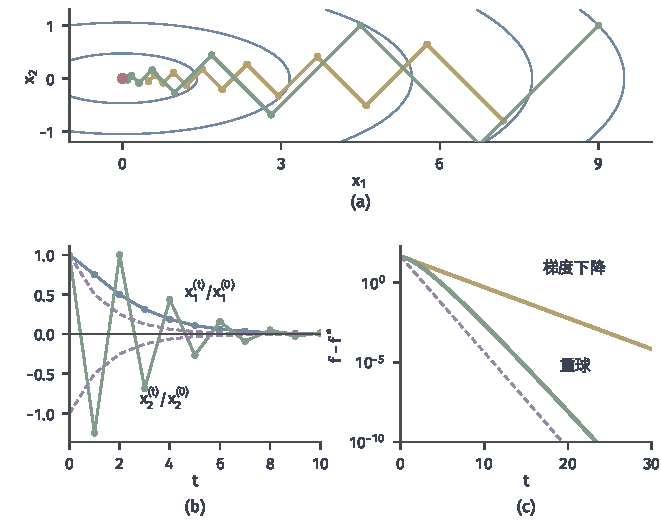
\includegraphics[width=112mm]{figures/05-optimization/02-smooth-optimization/matplotlib/fom-hb-paths/figure.pdf}
  \caption{贯穿例上的重球法（绿色，$\alpha=\beta=1/4$）与梯度下降（黄色，$\alpha=1/5$）。(a)等高线上的前$14$步。(b)重球法两坐标相对初值的比，式~\eqref{eq:fom-hb-closed}，紫色虚线是$\pm\rho^t$。(c)目标差的半对数曲线，紫色虚线是$45\rho^{2t}$，绿线在上方平行，差别来自多项式因子。}
  \label{fig:fom-hb-paths}
\end{BookInlineFigure}

所以，用$\rho$比较两种方法时，要记住它是渐近的说法。达到相对精度$\varepsilon$的步数约为$\tfrac{\sqrt\kappa}{2}\ln(1/\varepsilon)$，与梯度下降的$\tfrac\kappa2\ln(1/\varepsilon)$相比，$\kappa=10^4$时大约快一百倍。

\paragraph{参数的稳定范围}
这个加速依赖于参数对$L$和$\mu$的准确了解。由递推~\eqref{eq:fom-hb-scalar}的两根都在单位圆内的条件，可以写出稳定范围。多项式$p(r)=r^2-(1+\beta-\alpha\lambda)r+\beta$满足$p(1)=\alpha\lambda$，$p(-1)=2(1+\beta)-\alpha\lambda$，在$\beta\geq0$时，两根都在单位圆内当且仅当
\begin{equation}
 \beta<1,\qquad0<\alpha\lambda<2(1+\beta).
 \label{eq:fom-hb-stable}
\end{equation}

判据是$p(1)>0$，$p(-1)>0$，且根之积$\beta$的绝对值小于$1$。例中若沿用$\alpha=1/4$，却把$\beta$减到$0.06$，则$\alpha L=2.25$大于$2(1+\beta)=2.12$，陡峭方向发散。动量不只是“加速的旋钮”，它也放宽了步长的稳定界限，两个参数必须一起调。

\paragraph{离开二次目标}
式~\eqref{eq:fom-hb-params}的推导完全依赖于每个方向有固定的$\lambda$。目标不是二次时，局部曲率随位置变化，没有固定的特征方向。若$f$二阶连续可微，而$\bm{x}^\star$处的Hessian特征值落在$[\mu,L]$内，在$\bm{x}^\star$足够近处迭代可以用线性化来分析，局部收敛速度接近$\rho$；这是局部结论，对起点有要求。

全局情形下，这组参数确实可能失败。考虑一元函数，其导数分三段：
\begin{equation}
 f'(x)=\begin{cases}
 25x,&x<1,\\
 x+24,&1\leq x<2,\\
 25x-24,&x\geq2.
 \end{cases}
 \label{eq:fom-hb-counterexample}
\end{equation}
三段在分界点处衔接，$f'$连续且斜率都在$[1,25]$内，所以$f$强凸，$\mu=1$，$L=25$，最优解是$x^\star=0$。二次目标的最优参数是$\alpha=1/9$，$\beta=4/9$。

这组参数有一个周期为$3$的轨道，不会收敛：
\[
 x\text{ 依次取}\quad \frac{792}{1225},\quad-\frac{2208}{1225},\quad\frac{2592}{1225}.
\]

可以逐步核对。从前两点$2592/1225$（上一点）和$792/1225$（当前点）出发，当前点小于$1$，导数是$25x$。代入式~\eqref{eq:fom-hb}并把分母提出来：
\[
 x^{+}=\frac{1}{1225}\Bigl(792-\frac{25\cdot792}{9}+\frac49(792-2592)\Bigr)=-\frac{2208}{1225}.
\]

下一步当前点$-2208/1225$仍小于$1$，同样算得$2592/1225$。再下一步，当前点约为$2.116$，落在第三段，导数$25x-24$多出的常数$-24$提供了回拉，算得的新点恰好回到$792/1225$。

图~\ref{fig:fom-hb-cycle}展示了$x^{(0)}=3.3$时的情形：迭代很快落到这个周期上。作为对照，下一小节的方法在同一函数上正常收敛。这个反例说明，正定二次目标上的最优参数不能直接移到一般强凸目标上，也不能因此宣称全局加速。

\begin{BookInlineFigure}
  \centering
  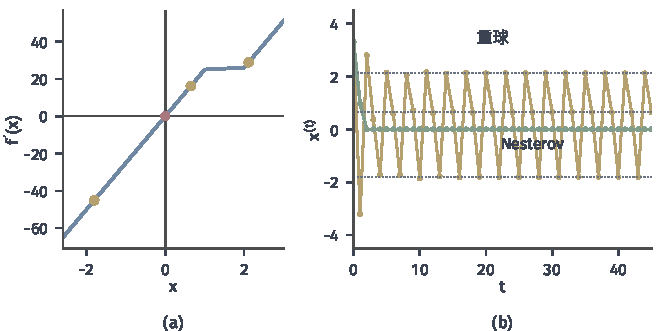
\includegraphics[width=112mm]{figures/05-optimization/02-smooth-optimization/matplotlib/fom-hb-cycle/figure.pdf}
  \caption{强凸光滑目标上重球法不收敛的例子。(a)式~\eqref{eq:fom-hb-counterexample}的导数$f'(x)$（蓝线），红点是最优解，黄点是周期轨道的三个点。(b)从$x^{(0)}=3.3$出发的迭代，黄线是重球法（$\alpha=1/9$，$\beta=4/9$），落到灰色点线标出的周期上；绿线是$\alpha=1/25$，$\beta=2/3$的Nesterov方法，收敛到$0$。}
  \label{fig:fom-hb-cycle}
\end{BookInlineFigure}

对一般强凸目标，缩小参数可以恢复全局收敛，但已知的这类分析一般达不到$\sqrt\kappa$的依赖，具体的条件和常数需要逐项核对，证明较长，读者可查阅一阶方法的专门文献。本章只在正定二次目标上给重球法下定量结论。

\subsection{Nesterov加速梯度法}
\label{sec:fom-nesterov}

\paragraph{主要思想}
重球法的动量盲目地累加：梯度在当前点读取，动量推出的位置却没有被检查，步子跨过谷底时也不会被纠正。一个自然的改进是把两件事的次序换一下：先顺着动量探出去，到探出的位置上再看坡度，用那里的梯度来修正。

这就是\term{Nesterov加速梯度法}（Nesterov accelerated gradient）\scite{nesterov1983method}。

它先由当前与历史迭代构成\term{外推点}（extrapolation point）$\bm{y}^{(t)}$，再在外推点做一步梯度下降：
\begin{equation}
 \begin{aligned}
 \bm{y}^{(t)}&=\bm{x}^{(t)}+\beta^{(t)}\bigl(\bm{x}^{(t)}-\bm{x}^{(t-1)}\bigr),\\
 \bm{x}^{(t+1)}&=\bm{y}^{(t)}-\alpha\nabla f(\bm{y}^{(t)}).
 \end{aligned}
 \label{eq:fom-nag}
\end{equation}
与式~\eqref{eq:fom-hb}比较，只有梯度的计算位置不同。图~\ref{fig:fom-nag-geometry}把一步的结构并排画出。

\begin{BookInlineFigure}
  \centering
  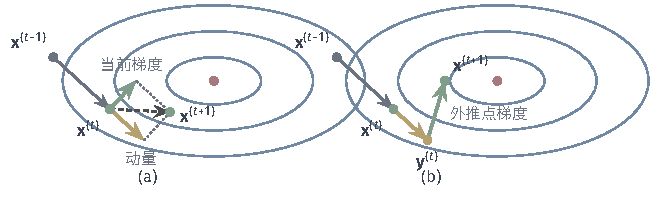
\includegraphics[width=110mm]{figures/05-optimization/02-smooth-optimization/tikz/fom-nag-geometry/figure.pdf}
  \caption{一步更新的结构对比，蓝色椭圆是等高线，红点是最优解。(a)重球法：动量（黄）和当前点的负梯度（绿）都从$\bm{x}^{(t)}$出发，两者相加得到新点。(b)Nesterov方法：先沿动量走到外推点$\bm{y}^{(t)}$，再从那里走一步负梯度。外推点已经冲到谷壁的外侧，那里的梯度把步子拉回。}
  \label{fig:fom-nag-geometry}
\end{BookInlineFigure}

用二次目标看这一改变的效果。代入$\nabla f(\bm{y})=\bm{H}(\bm{y}-\bm{x}^\star)$，并在特征方向上写开，记$s=1-\alpha\lambda$，得到
\begin{equation}
 e_\lambda^{(t+1)}=s\Bigl((1+\beta)e_\lambda^{(t)}-\beta e_\lambda^{(t-1)}\Bigr).
 \label{eq:fom-nag-scalar}
\end{equation}

对照式~\eqref{eq:fom-hb-scalar}。重球法的$-\beta e^{(t-1)}$不受$\lambda$影响，动量对各方向一视同仁；这里动量也被乘了$s$，曲率大的方向$s$小，动量被自动压低。这就是“外推点的梯度纠正动量”在公式上的含义。

特征方程是$r^2-s(1+\beta)r+s\beta=0$。复根时两根的积等于模的平方，所以模是$\sqrt{s\beta}$，随$\lambda$的增大而减小。

参数怎样选？取$\alpha=1/L$。例如强凸时取
\begin{equation}
 \beta=\frac{\sqrt\kappa-1}{\sqrt\kappa+1}.
 \label{eq:fom-nag-beta-strong}
\end{equation}
于是最平坦的方向$\lambda=\mu$上，$s=1-1/\kappa$，判别式恰好为零，二重根是$1-1/\sqrt\kappa$。由$(1+\beta)^2s=4\beta$可以直接验证这一点：把$\beta$代入，$(1+\beta)=2\sqrt\kappa/(\sqrt\kappa+1)$，$4\beta/(1+\beta)^2=(\kappa-1)/\kappa=s$。

而光滑凸时，$\mu$不可用，系数要随步数增长，后文的定理将说明它的具体形式。例中$\sqrt\kappa=3$，
\[
 \alpha=\frac19,\qquad\beta=\frac12,\qquad1-\frac{1}{\sqrt\kappa}=\frac23.
\]

\needspace{6\baselineskip}
\paragraph{变量}
\begin{itemize}
 \item $\bm{x}^{(t)},\bm{x}^{(t-1)}\in\mathbb{R}^n$：当前点与上一点。
 \item $\bm{y}^{(t)}\in\mathbb{R}^n$：外推点，梯度在这里读取，用后可覆盖。
 \item $\alpha$，$\beta^{(t)}$：步长和外推系数。
 \item $\varepsilon$，$T$：容差与最大步数。
\end{itemize}

\paragraph{初始化}
令$\bm{x}^{(-1)}=\bm{x}^{(0)}$，于是$\bm{y}^{(0)}=\bm{x}^{(0)}$。例中$\alpha=1/9$，$\beta=1/2$，容差$\varepsilon=10^{-3}$，
\[
 \bm{y}^{(0)}=\bm{x}^{(0)}=(9,1).
\]

\needspace{6\baselineskip}
\paragraph{每轮更新}
在第$t$轮：
\begin{enumerate}
 \item \textbf{外推。}由式~\eqref{eq:fom-nag}的第一行计算$\bm{y}^{(t)}$。例中第一轮
 \[
  \bm{y}^{(0)}=(9,1).
 \]
 \item \textbf{读取外推点梯度并更新。}由式~\eqref{eq:fom-nag}的第二行计算$\bm{x}^{(t+1)}$。例中第一轮
 \[
  \nabla f(\bm{y}^{(0)})=(9,9),\qquad\bm{x}^{(1)}=(9,1)-\tfrac19(9,9)=(8,0).
 \]

 例中第二轮的外推点和梯度是
 \[
  \bm{y}^{(1)}=(8,0)+\tfrac12(-1,-1)=(7.5,-0.5),\qquad\nabla f(\bm{y}^{(1)})=(7.5,-4.5),
 \]
 于是
 \[
  \bm{x}^{(2)}=(7.5,-0.5)-\tfrac19(7.5,-4.5)=\bigl(\tfrac{20}3,0\bigr).
 \]

 例中第三轮的外推点和梯度是
 \[
  \bm{y}^{(2)}=\bigl(\tfrac{20}3,0\bigr)+\tfrac12\bigl(-\tfrac43,0\bigr)=(6,0),\qquad\nabla f(\bm{y}^{(2)})=(6,0),
 \]
 于是
 \[
  \bm{x}^{(3)}=(6,0)-\tfrac19(6,0)=\bigl(\tfrac{16}3,0\bigr).
 \]
 \item \textbf{检查停止。}若新点的梯度大小不超过$\varepsilon$或已达$T$步，输出$\bm{x}^{(t+1)}$。这一检查要在$\bm{x}^{(t+1)}$处多读一次梯度，实际计算中常改用外推点的梯度大小，或每隔若干步才检查。例中第三轮$\lVert\nabla f(\bm{x}^{(3)})\rVert_2\approx5.33$，继续。
\end{enumerate}

例中第二坐标在第一步之后就是零，原因是陡峭方向$\lambda=L$上$s=0$，由式~\eqref{eq:fom-nag-scalar}，下一步的误差直接等于零。平坦方向的递推是$e^{(t+1)}=\tfrac43e^{(t)}-\tfrac49e^{(t-1)}$，二重根是$\tfrac23$，解出
\begin{equation}
 x_1^{(t)}=(9+3t)\Bigl(\frac23\Bigr)^t,\qquad x_2^{(t)}=0\quad(t\geq1).
 \label{eq:fom-nag-closed}
\end{equation}

代入式~\eqref{eq:fom-nag-closed}，第$29$步首次满足容差。最终得到
\[
 \bm{x}^{(29)}\approx(7.51\times10^{-4},\,0).
\]

\paragraph{强凸情形的势函数分析}
图~\ref{fig:fom-nag-paths}(b)比较了三种方法在例中各方向上的根，(c)是目标差。在这个二次例子上，重球法的因子$\tfrac12$比Nesterov方法的$\tfrac23$更小，步数$19$也少于$29$。Nesterov方法的价值不在于二次目标上最快，而在于它的保证可以一直延伸到一般的强凸光滑目标，而这正是重球法在式~\eqref{eq:fom-hb-counterexample}中失败的地方。

\begin{BookInlineFigure}
  \centering
  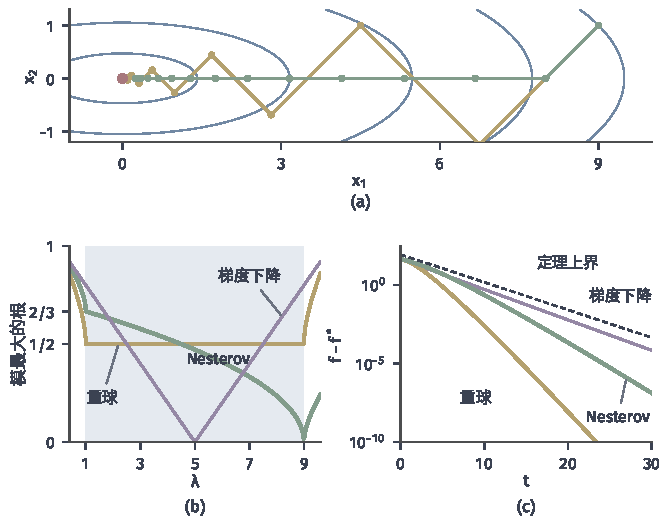
\includegraphics[width=112mm]{figures/05-optimization/02-smooth-optimization/matplotlib/fom-nag-paths/figure.pdf}
  \caption{贯穿例上的Nesterov方法（绿色，$\alpha=1/9$，$\beta=1/2$），对照重球法（黄色，$\alpha=\beta=1/4$）和梯度下降（紫色，$\alpha=1/5$）。(a)等高线上的前$14$步。(b)模最大的根关于$\lambda$的变化，蓝底区间是$[\mu,L]$。(c)目标差，黑色虚线是式~\eqref{eq:fom-nag-strong}给出的上界$86(2/3)^t$。}
  \label{fig:fom-nag-paths}
\end{BookInlineFigure}

要在一般目标上证明收敛，不能再用特征分解，也不能指望函数值单调下降：动量可能把函数值暂时抬高。需要另找一个每步都下降的量，称为\term{势函数}（potential function）。它把“函数值的差”和“某个辅助点到解的距离”加起来，走动时一项增大可以由另一项吸收。

设$q=1/\sqrt\kappa=\sqrt{\mu/L}$，引入辅助点序列$\bm{v}^{(0)}=\bm{x}^{(0)}$，
\begin{equation}
 \bm{v}^{(t+1)}=\bm{x}^{(t)}+\frac1q\bigl(\bm{x}^{(t+1)}-\bm{x}^{(t)}\bigr).
 \label{eq:fom-nag-v}
\end{equation}
它是沿本步位移放大$1/q$倍得到的“更大胆的点”。

\begin{theorem}[强凸情形的Nesterov方法]
\label{thm:fom-nag-strong}
设$f$的梯度$L$-Lipschitz连续且$\mu$强凸，$\mu>0$。取$\alpha=1/L$和式~\eqref{eq:fom-nag-beta-strong}的常数$\beta$，$\bm{x}^{(-1)}=\bm{x}^{(0)}$。则势函数
\begin{equation}
 \Phi^{(t)}=f(\bm{x}^{(t)})-f^\star+\frac\mu2\lVert\bm{v}^{(t)}-\bm{x}^\star\rVert_2^2
 \label{eq:fom-nag-potential}
\end{equation}
满足$\Phi^{(t+1)}\leq(1-1/\sqrt\kappa)\Phi^{(t)}$，因此
\begin{equation}
 f(\bm{x}^{(T)})-f^\star\leq\Bigl(1-\frac{1}{\sqrt\kappa}\Bigr)^T\Bigl(f(\bm{x}^{(0)})-f^\star+\frac\mu2\lVert\bm{x}^{(0)}-\bm{x}^\star\rVert_2^2\Bigr).
 \label{eq:fom-nag-strong}
\end{equation}
\end{theorem}

\begin{proof}
固定一步，省略上标$(t)$，记$\bm{g}=\nabla f(\bm{y})$，$\bm{x}^+$和$\bm{v}^+$为下一步的点。先把辅助点写成便于计算的形式。

第一步，验证两个恒等式：
\[
 \bm{y}=\frac{\bm{x}+q\bm{v}}{1+q},\qquad
 \bm{v}^+=(1-q)\bm{v}+q\bm{y}-\frac q\mu\bm{g}.
\]

第一式在$t=0$时成立。设它对$t$成立，则$q\bm{v}=(1+q)\bm{y}-\bm{x}$，代入第二式右端，并用$\frac{q}{\mu}=\frac{1}{qL}$和$\bm{x}^+=\bm{y}-\bm{g}/L$，化简得到
\[
 \frac1q\bigl(\bm{x}^+-(1-q)\bm{x}\bigr)=\bm{x}+\frac1q(\bm{x}^+-\bm{x}),
\]
正是式~\eqref{eq:fom-nag-v}。再把$\bm{v}^+$代入$(\bm{x}^++q\bm{v}^+)/(1+q)$，得到
\[
 \bm{x}^++\frac{1-q}{1+q}(\bm{x}^+-\bm{x})=\bm{y}^{(t+1)},
\]
所以第一式对$t+1$成立；这里用到$\beta=(1-q)/(1+q)$，它就是式~\eqref{eq:fom-nag-beta-strong}。

第二步，估计距离项。记$\bm{w}=(1-q)\bm{v}+q\bm{y}$，则$\bm{v}^+=\bm{w}-\frac q\mu\bm{g}$，展开平方并乘$\frac\mu2$：
\[
 \frac\mu2\lVert\bm{v}^+-\bm{x}^\star\rVert_2^2
 =\frac\mu2\lVert\bm{w}-\bm{x}^\star\rVert_2^2-q\bm{g}^\top(\bm{w}-\bm{x}^\star)+\frac{q^2}{2\mu}\lVert\bm{g}\rVert_2^2.
\]

第三步，函数项。由下降引理，外推点走一步满足
\[
 f(\bm{x}^+)\leq f(\bm{y})-\frac{1}{2L}\lVert\bm{g}\rVert_2^2.
\]

又$q^2/(2\mu)=1/(2L)$，两边的$\lVert\bm{g}\rVert_2^2$恰好抵消。再用平方范数的凸性拆开$\bm{w}$，得到
\[
 \Phi^{(t+1)}\leq f(\bm{y})-f^\star+(1-q)\frac\mu2\lVert\bm{v}-\bm{x}^\star\rVert_2^2+q\frac\mu2\lVert\bm{y}-\bm{x}^\star\rVert_2^2-q\bm{g}^\top(\bm{w}-\bm{x}^\star).
\]

第四步，处理内积。把$\bm{w}-\bm{x}^\star$拆开：
\[
 \bm{w}-\bm{x}^\star=(1-q)(\bm{v}-\bm{y})+(\bm{y}-\bm{x}^\star).
\]

对后一部分用强凸性：
\[
 q\bm{g}^\top(\bm{y}-\bm{x}^\star)\geq q\bigl(f(\bm{y})-f^\star\bigr)+q\frac\mu2\lVert\bm{y}-\bm{x}^\star\rVert_2^2.
\]
代入后，$\lVert\bm{y}-\bm{x}^\star\rVert_2^2$项抵消，留下
\[
 \Phi^{(t+1)}\leq(1-q)\bigl(f(\bm{y})-f^\star\bigr)+(1-q)\frac\mu2\lVert\bm{v}-\bm{x}^\star\rVert_2^2-q(1-q)\bm{g}^\top(\bm{v}-\bm{y}).
\]

第五步，由第一式$q(\bm{v}-\bm{y})=\bm{y}-\bm{x}$，末项等于$(1-q)\bm{g}^\top(\bm{x}-\bm{y})$。凸性给出
\[
 \bm{g}^\top(\bm{x}-\bm{y})\leq f(\bm{x})-f(\bm{y}),
\]
于是$f(\bm{y})$消去，
\[
 \Phi^{(t+1)}\leq(1-q)\Bigl(f(\bm{x})-f^\star+\frac\mu2\lVert\bm{v}-\bm{x}^\star\rVert_2^2\Bigr)=(1-q)\Phi^{(t)}.
\]

由$\bm{v}^{(0)}=\bm{x}^{(0)}$，迭代得
\[
 f(\bm{x}^{(T)})-f^\star\leq\Phi^{(T)}\leq(1-q)^T\Phi^{(0)}.
\]
\end{proof}

用贯穿例核对势函数。$\mu=1$，$q=\tfrac13$，辅助点由式~\eqref{eq:fom-nag-v}算出，三个势函数值依次是
\[
 \begin{aligned}
 \bm{v}^{(0)}&=(9,1), &\Phi^{(0)}&=45+41=86,\\
 \bm{v}^{(1)}&=(6,-2), &\Phi^{(1)}&=32+20=52,\\
 \bm{v}^{(2)}&=(4,0), &\Phi^{(2)}&\approx22.22+8=30.22.
 \end{aligned}
\]
定理要求每步至少缩小到$\tfrac23$：$86\cdot\tfrac23\approx57.3\geq52$，$52\cdot\tfrac23\approx34.7\geq30.22$。

强凸性给出距离项不超过初始目标差，所以式~\eqref{eq:fom-nag-strong}右端不超过初始目标差的$2(1-1/\sqrt\kappa)^T$倍。所以达到目标差$\varepsilon$的步数约为$\sqrt\kappa\ln(1/\varepsilon)$，与重球法在二次目标上的量级相同，但条件只要求一般的强凸光滑。式~\eqref{eq:fom-hb-counterexample}满足这些条件，定理保证了图~\ref{fig:fom-hb-cycle}中绿线的收敛。

\paragraph{光滑凸情形的势函数分析}
没有强凸常数时，常数的$\beta$无从定义。这时让外推系数随步数增长。定义
\begin{equation}
 \theta^{(0)}=1,\qquad\theta^{(t+1)}=\frac{1+\sqrt{1+4(\theta^{(t)})^2}}{2},\qquad
 \beta^{(t+1)}=\frac{\theta^{(t)}-1}{\theta^{(t+1)}},
 \label{eq:fom-nag-theta}
\end{equation}
并取$\beta^{(0)}=0$，$\alpha=1/L$。$\theta^{(t+1)}$是方程$\theta^2-\theta=(\theta^{(t)})^2$的正根，这个关系在证明中恰好让相邻两项抵消。由$\theta^{(t+1)}\geq\theta^{(t)}+\tfrac12$得$\theta^{(t)}\geq(t+2)/2$，系数$\beta^{(t)}$逐步趋近于$1$。

\begin{theorem}[光滑凸情形的Nesterov方法]
\label{thm:fom-nag-convex}
设$f$凸，梯度$L$-Lipschitz连续，存在最优解$\bm{x}^\star$。按式~\eqref{eq:fom-nag}、\eqref{eq:fom-nag-theta}迭代，$\alpha=1/L$，则对任意$T\geq1$，
\begin{equation}
 f(\bm{x}^{(T)})-f^\star\leq\frac{2L\lVert\bm{x}^{(0)}-\bm{x}^\star\rVert_2^2}{(T+1)^2}.
 \label{eq:fom-nag-convex}
\end{equation}
\end{theorem}

\begin{proof}
第一步，建立一个单步不等式。设$\bm{y}$任意，$\bm{x}^+=\bm{y}-\nabla f(\bm{y})/L$，$\bm{z}$任意。由下降引理和凸性，
\[
 f(\bm{x}^+)\leq f(\bm{z})+\nabla f(\bm{y})^\top(\bm{y}-\bm{z})-\frac{1}{2L}\lVert\nabla f(\bm{y})\rVert_2^2.
\]

把$\nabla f(\bm{y})=L(\bm{y}-\bm{x}^+)$代入，并用恒等式
\[
 2\bm{a}^\top\bm{b}-\lVert\bm{a}\rVert_2^2=\lVert\bm{b}\rVert_2^2-\lVert\bm{b}-\bm{a}\rVert_2^2,
\]
其中$\bm{a}=\bm{y}-\bm{x}^+$，$\bm{b}=\bm{y}-\bm{z}$，得到
\begin{equation}
 f(\bm{x}^+)-f(\bm{z})\leq\frac L2\Bigl(\lVert\bm{y}-\bm{z}\rVert_2^2-\lVert\bm{x}^+-\bm{z}\rVert_2^2\Bigr).
 \label{eq:fom-nag-one-step}
\end{equation}

第二步，选择比较点。省略上标$(t)$，记$\theta=\theta^{(t)}$，$\Delta_t=f(\bm{x}^{(t)})-f^\star$。取
\[
 \bm{z}=\Bigl(1-\frac1\theta\Bigr)\bm{x}+\frac1\theta\bm{x}^\star.
\]

由凸性，
\[
 f(\bm{z})-f^\star\leq\Bigl(1-\frac1\theta\Bigr)\Delta_t.
\]

代入式~\eqref{eq:fom-nag-one-step}，两边乘以$\theta^2$，把$\theta$乘进范数：
\[
 \theta^2\Delta_{t+1}-(\theta^2-\theta)\Delta_t\leq\frac L2\Bigl(\lVert\theta\bm{y}-\theta\bm{z}\rVert_2^2-\lVert\theta\bm{x}^+-\theta\bm{z}\rVert_2^2\Bigr).
\]

第三步，识别辅助点。令
\[
 \bm{v}^{(t)}=\theta^{(t)}\bm{y}^{(t)}-\bigl(\theta^{(t)}-1\bigr)\bm{x}^{(t)},
\]
于是
\[
 \theta\bm{y}-\theta\bm{z}=\bm{v}^{(t)}-\bm{x}^\star.
\]

而由式~\eqref{eq:fom-nag}和式~\eqref{eq:fom-nag-theta}，$\theta^{(t+1)}\bm{y}^{(t+1)}$可以写开，得到
\[
 \bm{v}^{(t+1)}=\bm{x}^{(t)}+\theta^{(t)}\bigl(\bm{x}^{(t+1)}-\bm{x}^{(t)}\bigr),
\]
这恰好是$\theta\bm{x}^+-\theta\bm{z}+\bm{x}^\star$。

第四步，定义势函数$E^{(t)}$并裂项。规定$\theta^{(-1)}=0$，令
\[
 E^{(t)}=\bigl(\theta^{(t-1)}\bigr)^2\Delta_t+\frac L2\lVert\bm{v}^{(t)}-\bm{x}^\star\rVert_2^2.
\]

由$\theta^2-\theta=(\theta^{(t-1)})^2$（$t=0$时两边都是零），上一步的不等式就是$E^{(t+1)}\leq E^{(t)}$。又$\bm{v}^{(0)}=\bm{x}^{(0)}$，所以
\[
 \bigl(\theta^{(T-1)}\bigr)^2\Delta_T\leq E^{(T)}\leq E^{(0)}=\frac L2\lVert\bm{x}^{(0)}-\bm{x}^\star\rVert_2^2.
\]

再用$\theta^{(T-1)}\geq(T+1)/2$，即得式~\eqref{eq:fom-nag-convex}。
\end{proof}

$1/T$变成了$1/T^2$。目标差要达到$\varepsilon$，步数从$LR^2/(2\varepsilon)$降到约$\sqrt{2L/\varepsilon}\,R$。图~\ref{fig:fom-nag-convex}(a)用一个三对角的二次函数验证这一点，它的特征值一路逼近零，强凸常数实际上帮不上忙。

\begin{BookInlineFigure}
  \centering
  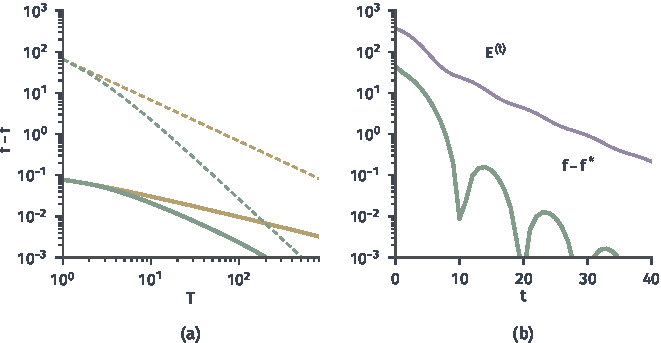
\includegraphics[width=112mm]{figures/05-optimization/02-smooth-optimization/matplotlib/fom-nag-convex/figure.pdf}
  \caption{光滑凸目标上的$1/T$与$1/T^2$。(a)$f(\bm{x})=\tfrac14(\tfrac12\bm{x}^\top\bm{A}\bm{x}-x_1)$，$\bm{A}$是$400$阶三对角矩阵（对角元$2$，次对角元$-1$），$L=1$，$\bm{x}^{(0)}=\bm{0}$。黄线是梯度下降，绿线是Nesterov方法（$\theta$形式），同色虚线是式~\eqref{eq:fom-gd-convex}、\eqref{eq:fom-nag-convex}的上界。(b)贯穿例按$\theta$形式运行，$L=9$：绿线是目标差，出现回升；紫线是势函数$E^{(t)}$，逐步下降。}
  \label{fig:fom-nag-convex}
\end{BookInlineFigure}

图~\ref{fig:fom-nag-convex}(b)说明势函数的用意。贯穿例按式~\eqref{eq:fom-nag-theta}的参数运行时，$\beta^{(t)}$逐渐接近$1$，动量过大，目标差出现$13$次回升，而$E^{(t)}$从$369$（$t=0$）、$320$（$t=1$）一路下降。凸情形的结论控制的是最后一步的目标差上界，并没有说目标差单调下降。

可以用势函数检查第一步的计算：由$\theta^{(0)}=1$得$\bm{v}^{(1)}=\bm{x}^{(1)}=(8,0)$，所以
\[
 E^{(1)}=1\cdot32+\frac92\cdot64=320,\qquad E^{(0)}=\frac92\cdot82=369.
\]

下表把两种动量方法放在一起对比。

\begin{BookInlineTable}
  \centering
  \caption{重球法与Nesterov方法的对比。}
  \label{tab:fom-momentum-compare}
  \begin{tabular}{lll}
   \toprule
   & 重球法 & Nesterov方法\\
   \midrule
   梯度位置 & 当前点$\bm{x}^{(t)}$ & 外推点$\bm{y}^{(t)}$\\
   动量对各方向 & 系数$\beta$相同 & 被$1-\alpha\lambda$压低\\
   $\alpha$ & $4/(\sqrt L+\sqrt\mu)^2$ & $1/L$\\
   强凸时$\beta$ & $\bigl(\frac{\sqrt\kappa-1}{\sqrt\kappa+1}\bigr)^2$ & $\frac{\sqrt\kappa-1}{\sqrt\kappa+1}$\\
   二次目标的速度 & $\frac{\sqrt\kappa-1}{\sqrt\kappa+1}$ & $1-1/\sqrt\kappa$\\
   一般强凸光滑 & 这组参数可能不收敛 & 定理~\ref{thm:fom-nag-strong}\\
   光滑凸 & 本章不给结论 & 定理~\ref{thm:fom-nag-convex}\\
   \bottomrule
  \end{tabular}
\end{BookInlineTable}

\paragraph{适用范围}
两条定理的证明都用切平面比较外推点与当前点、外推点与最优解，这正是凸性的作用。目标非凸时，切平面不再从下方托住目标，势函数的下降论证在第一步就不成立，这两条定理不能直接移用。非凸情形需要带函数值检查或重启的修改版本，另有专门的分析，得到的是驻点型的保证，本章不把上面的结论推广过去。

\section{非线性共轭梯度法}
\label{sec:fom-ncg}

上一节用历史位移修正步子，参数要事先知道$L$，有时还要知道$\mu$。本节换一种用历史的方式：每轮保留上一轮的搜索方向，把它与新梯度组合成新方向，步长由线搜索决定，不需要预先知道曲率常数。要解决的问题是：怎样组合才合理，这样组合之后还能保证什么？

先回到正定二次目标
\[
 f(\bm{x})=\frac12\bm{x}^\top\bm{H}\bm{x}-\bm{b}^\top\bm{x}.
\]

这里已经有一个答案：共轭梯度法。它的梯度$\bm{g}=\bm{H}\bm{x}-\bm{b}$就是残差的相反数，迭代为
\[
 \bm{d}^{(t)}=-\bm{g}^{(t)}+\beta^{(t)}\bm{d}^{(t-1)},\qquad
 \beta^{(t)}=\frac{\lVert\bm{g}^{(t)}\rVert_2^2}{\lVert\bm{g}^{(t-1)}\rVert_2^2},
\]
步长是沿$\bm{d}^{(t)}$的精确最小点。各方向两两关于$\bm{H}$共轭，精确算术下至多$n$步得到解。这些结论的推导可参考\BookChapterRef{chap:krylov-methods}{卷二第15章“Krylov子空间法”}。

共轭的意思是$(\bm{d}^{(i)})^\top\bm{H}\bm{d}^{(j)}=0$。用椭圆的语言说：把椭圆拉成圆后，这些方向互相垂直，所以沿一个方向走到位之后，后面的方向不会破坏已经完成的进度。图~\ref{fig:fom-sd-vs-cg}是贯穿例上的情形：最速下降在折返，共轭梯度第二步直接指向中心。

\begin{BookInlineFigure}
  \centering
  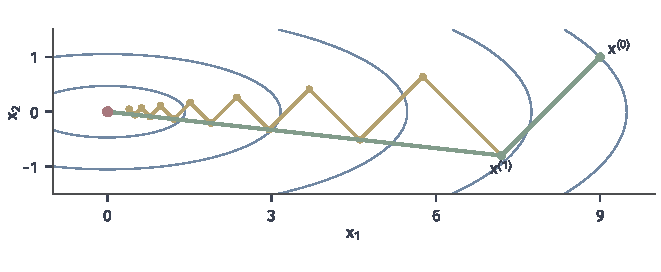
\includegraphics[width=112mm]{figures/05-optimization/02-smooth-optimization/matplotlib/fom-sd-vs-cg/figure.pdf}
  \caption{贯穿例上的精确线搜索路径，蓝色椭圆是等高线。黄色路径是最速下降，绿色路径是共轭梯度法。两者第一步相同，都到达$\bm{x}^{(1)}=(7.2,-0.8)$；共轭梯度的第二步到达最优解（红点），最速下降则继续折返。}
  \label{fig:fom-sd-vs-cg}
\end{BookInlineFigure}

目标不是二次时，两个前提都不存在：没有固定的$\bm{H}$，共轭的定义失去了依托；一般也求不出沿线的精确最小点。\term{非线性共轭梯度法}（nonlinear conjugate gradient method）只保留方向递推的形式，用真实的梯度代替残差，用线搜索代替精确步长。代价是，共轭性一般不再精确保持，有限步终止的结论也不再成立。

\subsection{方向的更新}
\label{sec:fom-ncg-direction}

\paragraph{主要思想}
方法的骨架是
\begin{equation}
 \bm{d}^{(t)}=-\bm{g}^{(t)}+\beta^{(t)}\bm{d}^{(t-1)},\qquad
 \bm{x}^{(t+1)}=\bm{x}^{(t)}+\alpha^{(t)}\bm{d}^{(t)},
 \label{eq:fom-ncg}
\end{equation}
其中$\bm{d}^{(0)}=-\bm{g}^{(0)}$。它只比梯度下降多存一个向量。需要决定的只有两件事：$\beta^{(t)}$怎样算，$\alpha^{(t)}$怎样选。这一小节讨论前者。

在二次目标上，$\beta^{(t)}$可以写成好几种形式，它们彼此相等。写法不同，推广到非线性时就成了不同的算法。从共轭条件出发，要求$(\bm{d}^{(t)})^\top\bm{H}\bm{d}^{(t-1)}=0$，由式~\eqref{eq:fom-ncg}得
\[
 \beta^{(t)}=\frac{(\bm{g}^{(t)})^\top\bm{H}\bm{d}^{(t-1)}}{(\bm{d}^{(t-1)})^\top\bm{H}\bm{d}^{(t-1)}}.
\]

式中含有$\bm{H}$，非线性时无法直接使用。在二次目标上，相邻梯度之差恰好是$\bm{H}$作用在位移上：
\[
 \bm{\delta}^{(t)}:=\bm{g}^{(t)}-\bm{g}^{(t-1)}=\alpha^{(t-1)}\bm{H}\bm{d}^{(t-1)}.
\]

把它代入上式，消去$\alpha^{(t-1)}$，得到只含梯度和方向的表达式：
\[
 \beta^{(t)}=\frac{(\bm{g}^{(t)})^\top\bm{\delta}^{(t)}}{(\bm{d}^{(t-1)})^\top\bm{\delta}^{(t)}}.
\]

精确线搜索使$(\bm{g}^{(t)})^\top\bm{d}^{(t-1)}=0$，并且同样有$(\bm{g}^{(t-1)})^\top\bm{d}^{(t-2)}=0$，由式~\eqref{eq:fom-ncg}得
\[
 (\bm{d}^{(t-1)})^\top\bm{\delta}^{(t)}=-(\bm{d}^{(t-1)})^\top\bm{g}^{(t-1)}=\lVert\bm{g}^{(t-1)}\rVert_2^2.
\]

这样分母化成了$\lVert\bm{g}^{(t-1)}\rVert_2^2$，得到\term{Polak--Ribière--Polyak公式}（Polak--Ribière--Polyak formula，PRP）：
\begin{equation}
 \beta_{\mathrm{PRP}}^{(t)}=\frac{(\bm{g}^{(t)})^\top\bigl(\bm{g}^{(t)}-\bm{g}^{(t-1)}\bigr)}{\lVert\bm{g}^{(t-1)}\rVert_2^2}.
 \label{eq:fom-beta-prp}
\end{equation}

再用线性共轭梯度中相邻梯度的正交性$(\bm{g}^{(t)})^\top\bm{g}^{(t-1)}=0$，分子只剩$\lVert\bm{g}^{(t)}\rVert_2^2$，得到\term{Fletcher--Reeves公式}（Fletcher--Reeves formula，FR）：
\begin{equation}
 \beta_{\mathrm{FR}}^{(t)}=\frac{\lVert\bm{g}^{(t)}\rVert_2^2}{\lVert\bm{g}^{(t-1)}\rVert_2^2}.
 \label{eq:fom-beta-fr}
\end{equation}

两个公式利用的信息不同。FR只看两个梯度的长度，恒为正；PRP还看梯度变化$\bm{\delta}^{(t)}$，它含有两点之间的曲率信息，符号可正可负。在正定二次目标加精确线搜索时两者一致，离开这个条件就是两个算法，下降性和收敛性要分别讨论。

\needspace{6\baselineskip}
\paragraph{变量}
\begin{itemize}
 \item $\bm{x}^{(t)}\in\mathbb{R}^n$：当前点。
 \item $\bm{g}^{(t)},\bm{g}^{(t-1)}\in\mathbb{R}^n$：当前与上一轮的梯度，FR只需要它们的长度平方，PRP需要向量。
 \item $\bm{d}^{(t)}\in\mathbb{R}^n$：搜索方向，算出新方向后覆盖。
 \item $\alpha^{(t)}$，$\beta^{(t)}$：步长与组合系数，用后即弃。
 \item $\varepsilon$，$T$：容差与最大步数。
\end{itemize}

\paragraph{初始化}
令$\bm{g}^{(0)}=\nabla f(\bm{x}^{(0)})$，$\bm{d}^{(0)}=-\bm{g}^{(0)}$，$t=0$。例中
\[
 \bm{g}^{(0)}=(9,9),\qquad\bm{d}^{(0)}=(-9,-9),\qquad\lVert\bm{g}^{(0)}\rVert_2^2=162.
\]

\needspace{6\baselineskip}
\paragraph{每轮更新}
在第$t$轮：
\begin{enumerate}
 \item \textbf{线搜索。}沿$\bm{d}^{(t)}$确定步长$\alpha^{(t)}$。这里先用精确步长，下一小节讨论实际的规则。二次目标的精确步长是
 \[
  \alpha^{(t)}=-\frac{(\bm{g}^{(t)})^\top\bm{d}^{(t)}}{(\bm{d}^{(t)})^\top\bm{H}\bm{d}^{(t)}}.
 \]
 例中第一轮
 \[
  \alpha^{(0)}=\frac{162}{(-9)^2\cdot1+(-9)^2\cdot9}=\frac{162}{810}=\frac15.
 \]

\item \textbf{更新点并读取新梯度。}由式~\eqref{eq:fom-ncg}得到$\bm{x}^{(t+1)}$，并计算$\bm{g}^{(t+1)}$。例中第一轮
 \[
  \bm{x}^{(1)}=(7.2,-0.8),\qquad\bm{g}^{(1)}=(7.2,-7.2).
 \]

\item \textbf{检查停止。}若$\lVert\bm{g}^{(t+1)}\rVert_2\leq\varepsilon$或已达$T$步，输出$\bm{x}^{(t+1)}$。例中第一轮$\lVert\bm{g}^{(1)}\rVert_2^2=103.68$，继续。

\item \textbf{计算系数并更新方向。}按式~\eqref{eq:fom-beta-fr}或式~\eqref{eq:fom-beta-prp}算$\beta^{(t+1)}$，再由式~\eqref{eq:fom-ncg}算$\bm{d}^{(t+1)}$，令$t\leftarrow t+1$。例中第一轮，$(\bm{g}^{(1)})^\top\bm{g}^{(0)}=0$，所以两个公式给出同一值：
 \[
  \beta^{(1)}=\frac{103.68}{162}=0.64.
 \]
 新方向是
 \[
  \bm{d}^{(1)}=(-7.2,7.2)+0.64(-9,-9)=(-12.96,\,1.44).
 \]
 可以核对共轭关系：
 \[
  (\bm{d}^{(1)})^\top\bm{H}\bm{d}^{(0)}=116.64-116.64=0.
 \]

 例中第二轮线搜索，方向导数和曲率分别是
 \[
  -(\bm{g}^{(1)})^\top\bm{d}^{(1)}=103.68,\qquad(\bm{d}^{(1)})^\top\bm{H}\bm{d}^{(1)}=186.624,
 \]
 于是
 \[
  \alpha^{(1)}=\frac{103.68}{186.624}=\frac59,\qquad
  \bm{x}^{(2)}=(7.2,-0.8)+\tfrac59(-12.96,1.44)=(0,0).
 \]
 此时$\bm{g}^{(2)}=\bm{0}$，满足停止条件。
\end{enumerate}

最终得到$\bm{x}^{(2)}=\bm{x}^\star$。二维的二次目标两步到达，这与$n$步终止的结论相符。图~\ref{fig:fom-ncg-direction}画出第二轮方向的合成：新梯度方向$-\bm{g}^{(1)}$与上一方向$\bm{d}^{(0)}$按平行四边形相加，结果恰好指向椭圆中心。

\begin{BookInlineFigure}
  \centering
  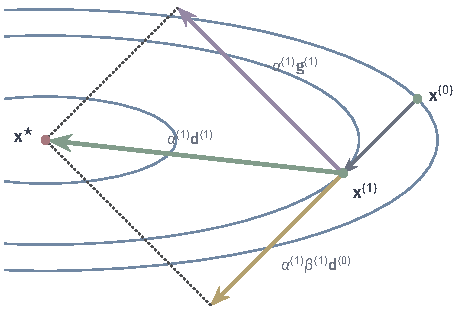
\includegraphics[width=80mm]{figures/05-optimization/02-smooth-optimization/tikz/fom-ncg-direction/figure.pdf}
  \caption{贯穿例第二轮的方向合成，蓝色椭圆是等高线。紫色箭头是负梯度$-\bm{g}^{(1)}$，黄色箭头是上一方向$\bm{d}^{(0)}$乘以$\beta^{(1)}=0.64$，两者都按步长$\alpha^{(1)}=5/9$缩放。绿色箭头是它们的和，从$\bm{x}^{(1)}$直达最优解（红点）。}
  \label{fig:fom-ncg-direction}
\end{BookInlineFigure}

\paragraph{两个公式何时不同}
精确线搜索一旦放宽，即使目标还是二次的，两个公式也立刻分开。在贯穿例第一轮取$\alpha^{(0)}=1/9$，它满足下一小节将列出的线搜索条件，于是
\[
 \bm{x}^{(1)}=(8,0),\qquad\bm{g}^{(1)}=(8,0),\qquad(\bm{g}^{(1)})^\top\bm{g}^{(0)}=72.
\]

这时相邻梯度不再正交。两个系数分别是
\[
 \beta_{\mathrm{FR}}^{(1)}=\frac{64}{162}\approx0.395,\qquad
 \beta_{\mathrm{PRP}}^{(1)}=\frac{64-72}{162}\approx-0.049.
\]

PRP的系数是负的，符号都不同了。对应的方向是
\[
 \bm{d}_{\mathrm{FR}}^{(1)}\approx(-11.56,\,-3.56),\qquad
 \bm{d}_{\mathrm{PRP}}^{(1)}\approx(-7.56,\,0.44).
\]
两者都不再与$\bm{d}^{(0)}$共轭，例如
\[
 (\bm{d}_{\mathrm{FR}}^{(1)})^\top\bm{H}\bm{d}^{(0)}=392\neq0.
\]
方程的形式相同，并不意味着结论相同。

目标非二次时，共轭性的流失更彻底。把贯穿例弯曲一下，取
\begin{equation}
 f(\bm{x})=\frac12x_1^2+\frac92\bigl(x_2-0.1x_1^2\bigr)^2.
 \label{eq:fom-bent}
\end{equation}
这是一条沿抛物线弯曲的山谷，$\bm{x}^\star=\bm{0}$处的Hessian仍是$\operatorname{diag}(1,9)$，系数$0.1$换成零就回到式~\eqref{eq:fom-example}。

图~\ref{fig:fom-ncg-bent}(b)用近乎精确的线搜索运行PRP，并计算相邻方向在当前Hessian下的共轭余弦。它在开始时接近$0.8$，远不是零；直到迭代进入极小点附近、目标接近二次，这个量才逐渐变小。这个二维问题走了$9$步才把梯度降到$10^{-6}$以下，$n$步终止不再成立。

\begin{BookInlineFigure}
  \centering
  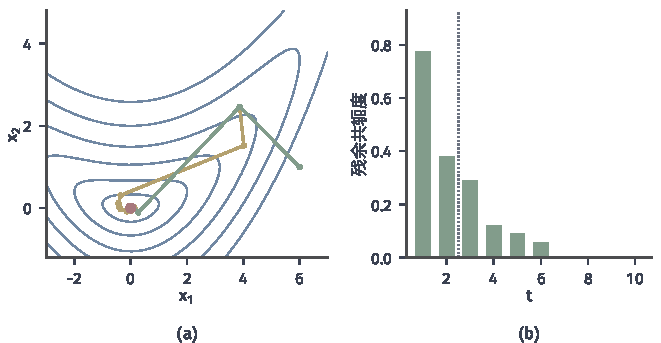
\includegraphics[width=112mm]{figures/05-optimization/02-smooth-optimization/matplotlib/fom-ncg-bent/figure.pdf}
  \caption{弯谷目标~\eqref{eq:fom-bent}上的非线性共轭梯度法，起点$(6,1)$。(a)黄线FR，绿线是把负的PRP系数截断为零的变体PRP+，都采用强Wolfe线搜索（$c_1=10^{-4}$，$c_2=0.4$），画出前$17$步。(b)近似精确线搜索下的PRP，相邻方向的残余共轭度$\lvert(\bm{d}^{(t)})^\top\nabla^2f\,\bm{d}^{(t-1)}\rvert$除以两方向的$\nabla^2f$长度之积，Hessian取在$\bm{x}^{(t)}$；虚线之前是二次目标应该结束的步数。}
  \label{fig:fom-ncg-bent}
\end{BookInlineFigure}

\subsection{线搜索与重启}
\label{sec:fom-ncg-linesearch}

\paragraph{强Wolfe条件}
实际中一般不求沿线精确的最小点。第~\ref{chap:smooth-foundations}章的强Wolfe条件要求步长$\alpha$既满足Armijo条件~\eqref{eq:fom-armijo}，又让方向导数的绝对值变小：
\begin{equation}
 \bigl\lvert\nabla f(\bm{x}+\alpha\bm{d})^\top\bm{d}\bigr\rvert\leq c_2\bigl\lvert\nabla f(\bm{x})^\top\bm{d}\bigr\rvert,\qquad 0<c_1<c_2<1.
 \label{eq:fom-strong-wolfe}
\end{equation}
前一个条件防止走得太远，后一个条件防止走得太近，同时把新点放到沿线函数接近平坦的位置。

贯穿例沿$\bm{d}^{(0)}=(-9,-9)$的一维函数是$\varphi(\alpha)=45-162\alpha+405\alpha^2$，方向导数为$\varphi'(\alpha)=-162+810\alpha$。取$c_1=0.1$，$c_2=0.45$，Armijo条件给出$\alpha\leq0.36$，强Wolfe条件给出
\[
 0.11\leq\alpha\leq0.29.
\]
图~\ref{fig:fom-wolfe}中，$\alpha=1/9$落在区间内，精确步长$1/5$也在区间内。

\begin{BookInlineFigure}
  \centering
  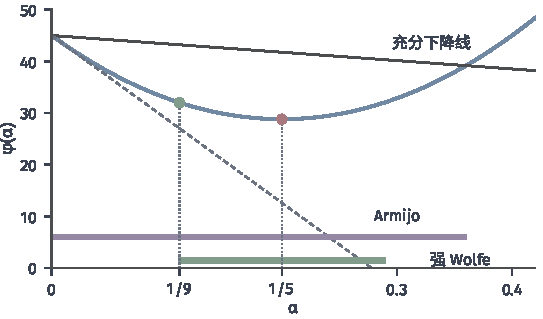
\includegraphics[width=92mm]{figures/05-optimization/02-smooth-optimization/matplotlib/fom-wolfe/figure.pdf}
  \caption{线搜索的可接受区间。蓝色曲线是贯穿例沿$\bm{d}^{(0)}$的$\varphi(\alpha)$，黑色实线是$c_1=0.1$的充分下降线，虚线是$\varphi$在$0$处的切线。紫色线段是Armijo条件接受的区间，绿色线段是再加上$c_2=0.45$的强Wolfe区间。绿点是$\alpha=1/9$，红点是精确最小点$\alpha=1/5$。}
  \label{fig:fom-wolfe}
\end{BookInlineFigure}

\paragraph{FR的下降保证}
方向必须是下降方向，线搜索才有意义。梯度下降中这是自动的，这里却不一定：$(\bm{g}^{(t)})^\top\bm{d}^{(t)}$等于$-\lVert\bm{g}^{(t)}\rVert_2^2$加上$\beta^{(t)}(\bm{g}^{(t)})^\top\bm{d}^{(t-1)}$，后一项可以是正的。精确线搜索让后一项为零；不精确时，强Wolfe条件要限制它的大小。对FR，这需要把$c_2$压到$\tfrac12$以下。

\begin{lemma}[FR方向的下降性]
\label{lem:fom-fr-descent}
设$f$连续可微，每步按强Wolfe条件取$\alpha^{(t)}$，$0<c_1<c_2<\tfrac12$，$\beta^{(t)}$取式~\eqref{eq:fom-beta-fr}，且$\bm{g}^{(t)}\neq\bm{0}$。则对所有$t$，
\begin{equation}
 -\frac{1}{1-c_2}\leq\frac{(\bm{g}^{(t)})^\top\bm{d}^{(t)}}{\lVert\bm{g}^{(t)}\rVert_2^2}\leq\frac{2c_2-1}{1-c_2}<0.
 \label{eq:fom-fr-descent}
\end{equation}
\end{lemma}

\begin{proof}
记中间的比值为$\tau^{(t)}$。对$t$归纳。$t=0$时$\tau^{(0)}=-1$，而
\[
 -\frac{1}{1-c_2}\leq-1\leq\frac{2c_2-1}{1-c_2},
\]
后一个不等号等价于$c_2\geq0$。

设结论对$t$成立，特别地$\bm{d}^{(t)}$是下降方向，线搜索可以进行。由式~\eqref{eq:fom-ncg}和$\beta_{\mathrm{FR}}^{(t+1)}$的定义，
\[
 \tau^{(t+1)}=-1+\frac{(\bm{g}^{(t+1)})^\top\bm{d}^{(t)}}{\lVert\bm{g}^{(t)}\rVert_2^2}.
\]

强Wolfe条件~\eqref{eq:fom-strong-wolfe}给出
\[
 \bigl\lvert(\bm{g}^{(t+1)})^\top\bm{d}^{(t)}\bigr\rvert\leq-c_2(\bm{g}^{(t)})^\top\bm{d}^{(t)}.
\]

除以$\lVert\bm{g}^{(t)}\rVert_2^2$，得到
\[
 -1+c_2\tau^{(t)}\leq\tau^{(t+1)}\leq-1-c_2\tau^{(t)}.
\]

代入归纳假设的下界$\tau^{(t)}\geq-1/(1-c_2)$，左端不小于$-1/(1-c_2)$，右端不大于$(2c_2-1)/(1-c_2)$。由$c_2<\tfrac12$，右端为负。
\end{proof}

用上面$\alpha^{(0)}=1/9$的数据检验。$c_2=0.45$时$\alpha^{(0)}$可接受，引理的区间是$[-1.82,-0.18]$，而
\[
 \tau^{(1)}=\frac{(8,0)^\top(-11.56,-3.56)}{64}\approx-1.44,
\]
确实落在区间内。

\paragraph{FR的全局收敛}
下降方向还不够，还要防止方向几乎与梯度垂直。记$\theta^{(t)}$为$\bm{d}^{(t)}$与$-\bm{g}^{(t)}$的夹角。Wolfe条件带来一个累加估计，它把线搜索的效果转化为对夹角的约束。

\begin{lemma}[Zoutendijk条件]
\label{lem:fom-zoutendijk}
设$f$有下界，梯度$L$-Lipschitz连续，$\bm{d}^{(t)}$都是下降方向，步长满足Armijo条件和Wolfe曲率条件（方向导数至少升到原值的$c_2$倍，$0<c_1<c_2<1$）。则
\begin{equation}
 \sum_{t=0}^\infty\cos^2\theta^{(t)}\lVert\bm{g}^{(t)}\rVert_2^2<\infty.
 \label{eq:fom-zoutendijk}
\end{equation}
\end{lemma}

\begin{proof}
曲率条件是
\[
 (\bm{g}^{(t+1)})^\top\bm{d}^{(t)}\geq c_2(\bm{g}^{(t)})^\top\bm{d}^{(t)}.
\]

两边减去$(\bm{g}^{(t)})^\top\bm{d}^{(t)}$，得到
\[
 (\bm{g}^{(t+1)}-\bm{g}^{(t)})^\top\bm{d}^{(t)}\geq(c_2-1)(\bm{g}^{(t)})^\top\bm{d}^{(t)}.
\]

由梯度Lipschitz，左端不超过$\alpha^{(t)}L\lVert\bm{d}^{(t)}\rVert_2^2$。于是步长有下界
\[
 \alpha^{(t)}\geq\frac{(1-c_2)\lvert(\bm{g}^{(t)})^\top\bm{d}^{(t)}\rvert}{L\lVert\bm{d}^{(t)}\rVert_2^2}.
\]

代入Armijo条件，并用$\lvert\bm{g}^\top\bm{d}\rvert$与$\cos\theta$的关系，得到
\[
 f(\bm{x}^{(t)})-f(\bm{x}^{(t+1)})\geq\frac{c_1(1-c_2)}{L}\cos^2\theta^{(t)}\lVert\bm{g}^{(t)}\rVert_2^2.
\]

对$t$求和，函数值裂项，再用下界，即得结论。
\end{proof}

\begin{theorem}[FR与强Wolfe线搜索]
\label{thm:fom-fr-convergence}
设$f$有下界，梯度$L$-Lipschitz连续。按FR公式迭代，步长满足强Wolfe条件，$0<c_1<c_2<\tfrac12$。若每步$\bm{g}^{(t)}\neq\bm{0}$，则
\begin{equation}
 \liminf_{t\to\infty}\lVert\bm{g}^{(t)}\rVert_2=0.
 \label{eq:fom-fr-convergence}
\end{equation}
\end{theorem}

\begin{proof}
用反证法。设存在$\gamma>0$使$\lVert\bm{g}^{(t)}\rVert_2\geq\gamma$对所有$t$成立。先估计方向的长度。由引理~\ref{lem:fom-fr-descent}，
\[
 \bigl\lvert(\bm{g}^{(t)})^\top\bm{d}^{(t)}\bigr\rvert\leq\frac{\lVert\bm{g}^{(t)}\rVert_2^2}{1-c_2}.
\]

再由强Wolfe条件，并用FR公式把$\beta^{(t+1)}\lVert\bm{g}^{(t)}\rVert_2^2$换成$\lVert\bm{g}^{(t+1)}\rVert_2^2$，展开$\lVert\bm{d}^{(t+1)}\rVert_2^2$，得到
\[
 \lVert\bm{d}^{(t+1)}\rVert_2^2\leq\frac{1+c_2}{1-c_2}\lVert\bm{g}^{(t+1)}\rVert_2^2+\bigl(\beta^{(t+1)}\bigr)^2\lVert\bm{d}^{(t)}\rVert_2^2.
\]

记$c=(1+c_2)/(1-c_2)\geq1$。两边除以$\lVert\bm{g}^{(t+1)}\rVert_2^4$，由FR公式消去$\beta^{(t+1)}$，因此
\[
 \frac{\lVert\bm{d}^{(t+1)}\rVert_2^2}{\lVert\bm{g}^{(t+1)}\rVert_2^4}\leq\frac{\lVert\bm{d}^{(t)}\rVert_2^2}{\lVert\bm{g}^{(t)}\rVert_2^4}+\frac{c}{\lVert\bm{g}^{(t+1)}\rVert_2^2}.
\]

由$\bm{d}^{(0)}=-\bm{g}^{(0)}$，归纳可得
\[
 \frac{\lVert\bm{d}^{(t)}\rVert_2^2}{\lVert\bm{g}^{(t)}\rVert_2^4}\leq\frac{c(t+1)}{\gamma^2}.
\]

再由引理~\ref{lem:fom-fr-descent}的上界，
\[
 \lvert\bm{g}^\top\bm{d}\rvert\geq c'\lVert\bm{g}\rVert_2^2,\qquad c'=\frac{1-2c_2}{1-c_2}>0.
\]
所以
\[
 \cos^2\theta^{(t)}\lVert\bm{g}^{(t)}\rVert_2^2=\frac{(\bm{g}^\top\bm{d})^2}{\lVert\bm{d}\rVert_2^2}\geq\frac{c'^2\lVert\bm{g}\rVert_2^4}{\lVert\bm{d}\rVert_2^2}\geq\frac{c'^2\gamma^2}{c(t+1)}.
\]

右端对$t$求和发散，与式~\eqref{eq:fom-zoutendijk}矛盾。
\end{proof}

定理不要求凸，结论是驻点型的，而且只是$\liminf$，说明有一列子序列的梯度趋于零。它与定理~\ref{thm:fom-gd-nonconvex}的$\lVert\bm{g}^{(t)}\rVert_2\to0$相比更弱，也不给出步数的界。

条件$c_2<\tfrac12$在这里是起作用的：引理的证明里，它让上界保持为负。一旦$c_2\geq\tfrac12$，上述论证不能保证方向下降。

\paragraph{FR的卡顿与PRP的自动重启}
定理保证了极限，却不保证速度。FR有一种典型的卡顿现象。若某一步步长很小，$\bm{g}^{(t)}\approx\bm{g}^{(t-1)}$，那么$\beta_{\mathrm{FR}}^{(t)}\approx1$，新方向约为$-\bm{g}^{(t)}+\bm{d}^{(t-1)}$，几乎沿用了旧方向。旧方向已经效果不佳，下一步又只能走很小的一步，如此延续。

PRP在同样的情形下，分子含有接近零的差$\bm{g}^{(t)}-\bm{g}^{(t-1)}$，于是$\beta_{\mathrm{PRP}}^{(t)}\approx0$，方向自动回到负梯度，相当于重新开始。这就是实践中PRP一般比FR好的原因。图~\ref{fig:fom-ncg-restart}在弯谷上对比了它们。

\begin{BookInlineFigure}
  \centering
  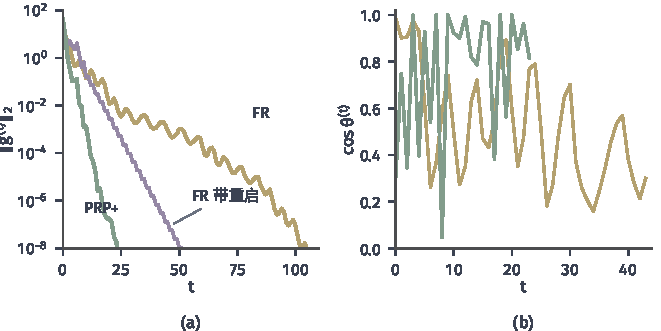
\includegraphics[width=112mm]{figures/05-optimization/02-smooth-optimization/matplotlib/fom-ncg-restart/figure.pdf}
  \caption{弯谷目标~\eqref{eq:fom-bent}上的三种方案，起点$(6,1)$，强Wolfe线搜索$c_1=10^{-4}$，$c_2=0.4$。(a)梯度大小：黄线是FR，紫线是FR加Powell重启（式~\eqref{eq:fom-powell-restart}，$\nu=0.1$），绿线是PRP+。(b)$\bm{d}^{(t)}$与$-\bm{g}^{(t)}$的夹角余弦：黄线FR在后期长时间偏低，绿线PRP+能够多次回到接近$1$的位置。}
  \label{fig:fom-ncg-restart}
\end{BookInlineFigure}

\paragraph{PRP+的下降保障}
PRP的优点有代价。Powell构造过非凸的例子，PRP配合精确线搜索也可能在一组非驻点之间循环，这说明全局收敛不能指望公式本身。这样的反例需要专门构造，证明的细节读者可查阅\scite{math-nocedal2006numerical}。

一个常用的修改是把负的系数截断为零：
\begin{equation}
 \beta_{\mathrm{PRP+}}^{(t)}=\max\bigl\{\beta_{\mathrm{PRP}}^{(t)},\,0\bigr\}.
 \label{eq:fom-beta-prp-plus}
\end{equation}
其含义是：若梯度变化表明上一方向已不再有帮助，就直接扔掉它。贯穿例上$\alpha^{(0)}=1/9$的那一步，PRP+的$\beta$就是$0$，新方向是负梯度$(-8,0)$。

只截断还不够。与FR不同，PRP+在强Wolfe条件下并不自动产生下降方向，因为$\beta$的大小不再受$\lVert\bm{g}^{(t)}\rVert_2^2/\lVert\bm{g}^{(t-1)}\rVert_2^2$限制。已知的收敛定理要求额外的条件：$f$的下水平集有界，梯度Lipschitz，线搜索除强Wolfe条件之外还要保证充分下降，即存在$c>0$使
\begin{equation}
 (\bm{g}^{(t)})^\top\bm{d}^{(t)}\leq-c\lVert\bm{g}^{(t)}\rVert_2^2.
 \label{eq:fom-sufficient-descent}
\end{equation}
在这些条件下可以得到$\liminf\lVert\bm{g}^{(t)}\rVert_2=0$。证明要追踪归一化方向的变化量并作累计估计，篇幅较长，读者可查阅\scite{math-nocedal2006numerical}。这个结论本章没有证明，它依赖的是“PRP+、线搜索与充分下降”三者的组合，缺一项就不能引用。

\paragraph{重启}
非线性情形下，旧方向携带的曲率信息随着地形变化而过期。\term{重启}（restart）就是把方向重置为负梯度，丢弃旧方向。常用的触发条件有三种。

第一种检测方向不再下降：若新方向不满足式~\eqref{eq:fom-sufficient-descent}，立即令$\bm{d}^{(t)}=-\bm{g}^{(t)}$。第二种按周期：每$n$步重启一次，相当于让方向序列按段重新建立。第三种由Powell提出，检测相邻梯度偏离了线性共轭梯度中的正交性：若
\begin{equation}
 \bigl\lvert(\bm{g}^{(t)})^\top\bm{g}^{(t-1)}\bigr\rvert\geq\nu\lVert\bm{g}^{(t)}\rVert_2^2,\qquad\nu\approx0.1,
 \label{eq:fom-powell-restart}
\end{equation}
就重启。

重启并不总是有益的。图~\ref{fig:fom-ncg-restart}(a)的数据是：从$(6,1)$出发，目标梯度$10^{-8}$，FR走了$105$步，加上重启后降到$52$步，PRP+只要$24$步。而对PRP+再加上式~\eqref{eq:fom-powell-restart}，在贯穿起点$(9,1)$上反而从$28$步增加到$52$步，因为PRP+本身已经在需要时自动重置，额外的重启浪费了仍然有用的方向。

下表把变体、线搜索和保证的组合列在一起。引用某个结论时，三列必须同时对应。

\begin{BookInlineTable}
  \centering
  \caption{非线性共轭梯度的常见组合，表中收敛都是$\liminf\lVert\bm{g}^{(t)}\rVert_2=0$。}
  \label{tab:fom-ncg-combos}
  \begin{tabular}{lll}
   \toprule
   变体 & 线搜索与附加条件 & 下降性与收敛\\
   \midrule
   FR & 强Wolfe，$c_2<\tfrac12$ & 下降，定理~\ref{thm:fom-fr-convergence}\\
   PRP & 精确或强Wolfe & 可能循环，无一般保证\\
   PRP+ & 强Wolfe，式~\eqref{eq:fom-sufficient-descent} & 收敛，本章未证\\
   加重启 & 依所用变体 & 保证随所用规则核对\\
   \bottomrule
  \end{tabular}
\end{BookInlineTable}

\section{收敛与计算成本}
\label{sec:fom-cost}

前三节各自给出了保证和例子。于是要问：要在几种方法中选择时，应该按什么标准比较？按第~\ref{chap:smooth-foundations}章的约定，比较时要固定三件事：度量误差的量、停止精度和要报告的迭代点，然后计算达到这一精度所需的总计算。

\paragraph{同样的尺子}
贯穿例上，以梯度大小不超过$10^{-3}$为停止标准，各方法的结果如下表。固定步长的方法每步读一次梯度，读取次数与步数大体相等。

\begin{BookInlineTable}
  \centering
  \caption{贯穿例上达到$\lVert\bm{g}\rVert_2\leq10^{-3}$的步数。}
  \label{tab:fom-example-count}
  \begin{tabular}{lll}
   \toprule
   方法 & 参数 & 步数\\
   \midrule
   梯度下降 & $\alpha=1/9$ & $78$\\
   梯度下降 & $\alpha=1/5$ & $43$\\
   重球法 & $\alpha=\beta=1/4$ & $19$\\
   Nesterov方法 & $\alpha=1/9$，$\beta=1/2$ & $29$\\
   共轭梯度 & 精确线搜索 & $2$\\
   \bottomrule
  \end{tabular}
\end{BookInlineTable}

这张表不能拿来宣布胜负。共轭梯度的$2$步依赖于目标是二次的，而且精确步长用到了$\bm{H}$；重球法的$19$步依赖于事先知道$\mu$和$L$，并且只对二次目标有理论保证；三种固定步长的方法都不必做线搜索。下面把这些差异分别计入。

\paragraph{保证的比较}
下表汇总本章的保证，$R=\lVert\bm{x}^{(0)}-\bm{x}^\star\rVert_2$，$\Delta=f(\bm{x}^{(0)})-f_{\inf}$。不同列的度量不同：非凸列是梯度大小，凸与强凸列是目标差。

\begin{BookInlineTable}
  \centering
  \caption{各方法的理论保证，$\Phi^{(0)}=f(\bm{x}^{(0)})-f^\star+\tfrac\mu2R^2$，“—”表示本章不给结论。}
  \label{tab:fom-guarantees}
  \begin{tabular}{llll}
   \toprule
   方法 & 非凸 & 凸 & 强凸\\
   \midrule
   梯度下降 & $\min\lVert\bm{g}\rVert_2^2\leq\frac{2L\Delta}{T}$ & $\frac{LR^2}{2T}$ & $(1-\frac1\kappa)^T\Delta$\\
   重球法 & — & — & 二次目标$(2T+1)\rho^T$\\
   Nesterov方法 & — & $\frac{2LR^2}{(T+1)^2}$ & $(1-\frac{1}{\sqrt\kappa})^T\Phi^{(0)}$\\
   FR & $\liminf\lVert\bm{g}\rVert_2=0$ & 同左 & 同左\\
   \bottomrule
  \end{tabular}
\end{BookInlineTable}

重球法一行的界是解距离的比例，$\rho=(\sqrt\kappa-1)/(\sqrt\kappa+1)$。FR的“同左”表示在凸和强凸情形下，本章的定理仍然只给出驻点型的结论。这与实际的快慢不是一回事：FR在实践中常比梯度下降快，但本章的定理没有给出这一点。

$T$与$\kappa$的影响可以换算成具体的数字。取$\kappa=10^4$，目标差要降到初值的$10^{-6}$，$\ln10^6\approx13.8$，于是
\[
 \kappa\ln\frac1\varepsilon\approx1.38\times10^5,\qquad
 \sqrt\kappa\ln\frac1\varepsilon\approx1.38\times10^3.
\]

相差一百倍。这是梯度下降与加速方法在定理的上界上的差别。Nesterov方法的$\sqrt\kappa$和$1/T^2$依赖，在“新迭代点只在已读取梯度的张成空间内”这类方法中不能进一步改进；证明需要构造一个三对角的二次函数，让前$T$步的梯度只能探到前$T$个坐标，篇幅较长，读者可查阅凸优化的专门著作。图~\ref{fig:fom-nag-convex}所用的函数正是这种构造。

\paragraph{一步要花多少}
迭代次数只是总计算的一个因子。每步的代价由三部分构成：梯度读取、线搜索的函数试探、向量的更新与存储。

\begin{BookInlineTable}
  \centering
  \caption{每步的代价，维数为$n$。}
  \label{tab:fom-cost-per-step}
  \begin{tabular}{llll}
   \toprule
   方法 & 梯度读取 & 存储向量 & 需要的信息\\
   \midrule
   梯度下降（固定） & $1$ & $2$ & $L$\\
   梯度下降（回溯） & $1$加试探 & $2$ & 无\\
   重球法 & $1$ & $3$ & $L,\mu$\\
   Nesterov方法 & $1$ & $3$ & $L$，强凸时加$\mu$\\
   非线性共轭梯度 & 多次 & $3$到$4$ & 无\\
   \bottomrule
  \end{tabular}
\end{BookInlineTable}

向量更新都是$O(n)$，与读一次梯度相比通常可以忽略。除非目标是高度结构化的，读一次梯度的代价要大得多。所以比较的主要量是梯度与函数的读取次数，而不是迭代步数。

强Wolfe线搜索每步要在试探点上计算函数值和方向导数，后者需要整个梯度，一次试探大约相当于一次完整的梯度读取。试探次数取决于初始步长的猜测和$c_2$的松紧。例如弯谷上$c_2=0.4$时，PRP+走了$24$步，用了$75$次读取，平均每步约$3$次。

\paragraph{步数少不等于计算少}
图~\ref{fig:fom-cost}在一个$100$维的问题上比较四种方法：
\[
 f(\bm{x})=\frac12\sum_{i=1}^{100}\lambda_ix_i^2+\sum_{i=1}^{100}\ln\cosh x_i,
\]
其中$\lambda_i$在$[1,1000]$内按对数等距分布。目标强凸，$\mu=1$，$L=1001$，要求$\lVert\bm{g}\rVert_2\leq10^{-6}$。

\begin{BookInlineFigure}
  \centering
  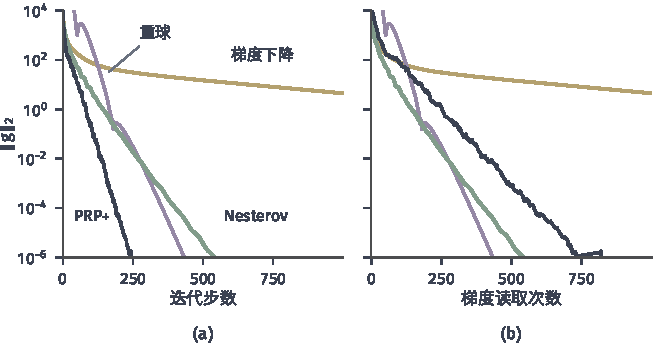
\includegraphics[width=112mm]{figures/05-optimization/02-smooth-optimization/matplotlib/fom-cost/figure.pdf}
  \caption{$100$维强凸非二次目标上的梯度大小，$\kappa=1001$，起点由固定种子的正态随机数给出。黄线是$\alpha=1/L$的梯度下降，紫线是按式~\eqref{eq:fom-hb-params}取参数的重球法，绿线是强凸参数的Nesterov方法，黑线是PRP+配合强Wolfe线搜索（$c_1=10^{-4}$，$c_2=0.1$）。(a)横轴是迭代步数。(b)横轴是梯度读取次数，同一组数据的位置变了。}
  \label{fig:fom-cost}
\end{BookInlineFigure}

按迭代步数，PRP+最少，$244$步，重球法$434$步，Nesterov方法$542$步，梯度下降$7574$步。按梯度读取，PRP+用了$821$次，比重球法的$435$次和Nesterov方法的$543$次都多。只看左图会选PRP+，只看右图会选重球法。

这张图也提醒另一点。重球法在这里表现好，但定理不保证它：目标不是二次的。Nesterov方法多读了约百分之二十五的梯度，换来的是对这一类目标有定理保证。四种配置中只有PRP+不需要$L$和$\mu$。这两个常数无法估计时，它可以直接运行；梯度下降配回溯也能做到这一点，只是更慢。

\paragraph{输出什么}
最后要说明报告哪个点。按定理~\ref{thm:fom-gd-nonconvex}的说法，非凸时应记录梯度最小的迭代点；凸与强凸的定理针对最后一个迭代点。Nesterov方法的目标差不单调，如果需要，可以另外保留函数值最低的点，这只需要在已经计算函数值时比较。

非线性共轭梯度的$\liminf$结论并不保证最后一点最好，同样应保留历史最优点。无论哪种方法，宣布达到精度之前都应该在输出点处重新计算一次梯度，而不是用外推点的梯度代替，后者并不是输出点的残差。

\section{本章小结}
\label{sec:fom-summary}

本章在只有函数值和梯度的条件下回答了“朝哪走、走多远、用不用历史”。负梯度是局部最陡的方向，二次上界决定一步能走多远，$\alpha=1/L$保证每步下降。梯度下降的保证按假设分三档：非凸时梯度变小，凸时目标差按$1/T$，强凸时按$(1-1/\kappa)^T$。

病态的目标让步长被陡峭方向限制，平坦方向进展缓慢，步数与$\kappa$成正比。历史位移可以把一致的方向累积起来，把振荡的方向抵消。重球法在当前点读取梯度，在正定二次目标上把各方向的收缩因子拉平为$(\sqrt\kappa-1)/(\sqrt\kappa+1)$，但这组参数离开二次目标可能循环。Nesterov方法把梯度移到外推点，用势函数得到强凸时的$(1-1/\sqrt\kappa)^T$和凸时的$1/T^2$，适用于一般的光滑目标，但函数值不必单调，目标非凸时定理不适用。

非线性共轭梯度保留上一方向，用线搜索决定步长，不需要曲率常数。FR配合$c_2<\tfrac12$的强Wolfe条件保证下降和$\liminf\lVert\bm{g}^{(t)}\rVert_2=0$，容易卡顿；PRP能自动重置，但需要PRP+、充分下降或重启等附加规则才能谈收敛。正定二次目标上的共轭性和有限步终止，在非线性目标上都不能照搬。

比较这些方法时，保证的条件和度量必须对应，成本要按梯度读取和线搜索试探计入，迭代次数少不等于总计算少。这些方法对局部曲率的利用都是间接的：历史位移和梯度差只是曲率的影子。如果能直接计算或近似局部曲率，更新方向可以由二次模型给出，下一章由此建立Newton方向。


\chapter{二阶方法}
\label{chap:second-order-methods}

沿一条狭长的山谷下山，只看脚下的坡度是很吃亏的。坡度告诉我们哪边低，却不告诉我们这面坡还能延续多远：陡的方向走一点就到了谷底另一侧，缓的方向走很远才有变化。第~\ref{chap:first-order-methods}章的方法靠步长和历史信息来缓解这种不匹配。假如还能读到二阶导数，就可以直接知道每个方向弯得有多厉害，并据此决定走多远。

本章研究这样得到的方法。出发点只有一句话：在当前点用二次函数近似目标，然后走到这个二次函数的极小点。第~\ref{sec:newton-basic}节由此导出Newton法，并说明它在解附近为什么快得惊人。

这句话照字面执行会遇到三种麻烦。离解很远时，二次函数和目标相差太大，走到它的极小点可能反而更差。曲率矩阵可能不正定，这时“二次函数的极小点”根本不存在。维数很高时，解一次线性方程本身就可能算不起。

三种麻烦分别由后面三节处理。第~\ref{sec:newton-damped}节不改方向，只缩短步长。第~\ref{sec:newton-modified}节改变曲率矩阵，让方向重新可用。第~\ref{sec:newton-inexact}节允许线性方程解得不精确，并规定解到什么程度够用。三种手段针对不同的困难，可以单独使用，也可以组合。第~\ref{sec:newton-cost}节把它们放到相同的精度标准下，比较从起点到终点的全部计算量。

\section{Newton法}
\label{sec:newton-basic}

手里有当前点的梯度和Hessian，下一步应该走到哪里，这样走在什么条件下是对的，又能快到什么程度？

\paragraph{用一个碗代替地形}
设$f:\mathbb{R}^n\to\mathbb{R}$二阶连续可微。站在$\bm{x}^{(t)}$处，把目标在附近作二阶Taylor展开，保留到二次项，得到\term{局部二次模型}（local quadratic model）
\begin{equation}
 m^{(t)}(\bm{d})=f(\bm{x}^{(t)})+(\bm{g}^{(t)})^\top\bm{d}+\frac12\bm{d}^\top\bm{H}^{(t)}\bm{d},
 \label{eq:newton-model}
\end{equation}
其中$\bm{d}$是从当前点出发的位移，$\bm{g}^{(t)}=\nabla f(\bm{x}^{(t)})$，$\bm{H}^{(t)}=\nabla^2f(\bm{x}^{(t)})$。Taylor公式的余项估计可参考\BookChapterRef{chap:multivariate-differentiation}{卷二第20章“多元函数微分”}。

模型和目标在当前点有相同的函数值、斜率和弯曲程度。可以这样想：我们看不到整片地形，只能摸清脚下这一小块的坡度和弯度，于是用一只形状相同的碗去贴合脚下的地面。一阶方法只用一块斜板贴合，斜板告诉我们往哪边倒，却没有底；碗有底，底的位置就是模型给出的下一步。

这个比喻要记住它的限度。碗只在脚下贴合，$\lVert\bm{d}\rVert_2$越大，碗和地形的差别越大。后面几节的大部分工作都是在回答同一个问题：这只碗能信多远。

\paragraph{Newton方程}
当$\bm{H}^{(t)}$正定时，模型是真正的碗，它的底由模型梯度为零确定。对式~\eqref{eq:newton-model}关于$\bm{d}$求梯度并令其为零，得到
\begin{equation}
 \bm{H}^{(t)}\bm{d}^{(t)}=-\bm{g}^{(t)}.
 \label{eq:newton-equation}
\end{equation}
这个线性方程称为\term{Newton方程}（Newton equation），解$\bm{d}^{(t)}$称为\term{Newton方向}（Newton direction）。走满这一步就是\term{Newton法}（Newton's method）：
\begin{equation}
 \bm{x}^{(t+1)}=\bm{x}^{(t)}+\bm{d}^{(t)}.
 \label{eq:newton-update}
\end{equation}
实际计算解方程~\eqref{eq:newton-equation}，不求$(\bm{H}^{(t)})^{-1}$。对称正定方程用Cholesky分解，稠密时约$n^3/3$次运算；分解和回代的做法可参考\BookChapterRef{chap:direct-linear-solvers}{卷二第12章“线性方程的直接求解”}。

一元时方程~\eqref{eq:newton-equation}就是$f''(x)d=-f'(x)$。以$f(x)=e^x-2x$为例，最小点是$x^\star=\ln2\approx0.6931$。这时$f'(x)=e^x-2$，$f''(x)=e^x$，更新为
\[
 x^{(t+1)}=x^{(t)}-\frac{e^{x^{(t)}}-2}{e^{x^{(t)}}}=x^{(t)}-1+2e^{-x^{(t)}}.
\]
从$x^{(0)}=1.5$出发，
\[
 x^{(1)}=1.5-1+2e^{-1.5}\approx0.9463.
\]
一步就把误差从$0.807$降到$0.253$。

\begin{BookInlineFigure}
  \centering
  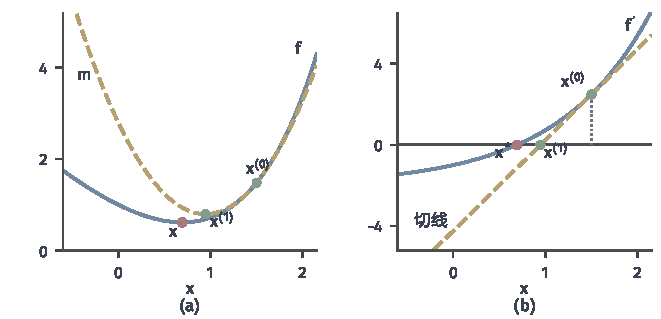
\includegraphics[width=112mm]{figures/05-optimization/02-smooth-optimization/matplotlib/newton-model-1d/figure.pdf}
  \caption{Newton步的两种读法，目标为$f(x)=e^x-2x$，$x^{(0)}=1.5$。(a)蓝线是目标，黄色虚线是在$x^{(0)}$处的二次模型，绿点$x^{(1)}$是模型的极小点，红点是真正的最小点$x^\star$。(b)蓝线是导数$f'$，黄色虚线是它在$x^{(0)}$处的切线，切线与横轴的交点正是同一个$x^{(1)}$。}
  \label{fig:newton-model-1d}
\end{BookInlineFigure}

图~\ref{fig:newton-model-1d}给出同一步的两种读法。图(a)是极小化的读法：用抛物线代替曲线，走到抛物线的底。图(b)是解方程的读法：要找$\nabla f=\bm{0}$的根，就把$\nabla f$在当前点线性化，再求线性函数的根。多元时，线性化$\nabla f(\bm{x}^{(t)}+\bm{d})\approx\bm{g}^{(t)}+\bm{H}^{(t)}\bm{d}$再令其为零，得到的仍是式~\eqref{eq:newton-equation}。

两种读法在正定时一致，但解方程的读法只找驻点，分不清极小点、极大点和鞍点。在$\bm{H}^{(t)}$不正定的地方，两者会分道扬镳，这正是下面要讲的。

\paragraph{贯穿全章的例子}
后面用同一个二元目标检验各种方法：
\begin{equation}
 f(\bm{x})=\frac12(x_1-1)^2+(x_2-x_1^2)^2.
 \label{eq:newton-running-objective}
\end{equation}
两个平方项同时为零当且仅当$\bm{x}=(1,1)$，所以$\bm{x}^\star=(1,1)$，$f^\star=0$。第二项把点拉向抛物线$x_2=x_1^2$，第一项才沿抛物线把点推向解，因此等高线是一条弯曲的山谷。

记$u=x_2-x_1^2$。逐项求导，得到梯度和Hessian：
\begin{equation}
 \nabla f(\bm{x})=\begin{bmatrix}x_1-1-4x_1u\\2u\end{bmatrix},\qquad
 \nabla^2f(\bm{x})=\begin{bmatrix}1-4u+8x_1^2&-4x_1\\-4x_1&2\end{bmatrix}.
 \label{eq:newton-running-derivatives}
\end{equation}
Hessian的右下角元素是$2>0$，行列式为
\[
 \det\nabla^2f(\bm{x})=2(1-4u+8x_1^2)-16x_1^2=2(1-4u).
\]
所以$\nabla^2f(\bm{x})$正定当且仅当$1-4u>0$，也就是点在抛物线$x_2=x_1^2+\tfrac14$的下方。这条抛物线上方的区域里Hessian不定，下面的图都用红色浅底标出。

这个例子的Newton方程能手解。由第二行得$d_2=-u+2x_1d_1$，代入第一行，含$8x_1^2$的项互相抵消，只剩$(1-4u)d_1=1-x_1$。于是，当$1-4u\neq0$时，
\begin{equation}
 d_1=\frac{1-x_1}{1-4u},\qquad d_2=-u+2x_1d_1.
 \label{eq:newton-running-direction}
\end{equation}

图~\ref{fig:newton-model-trust}比较模型和目标。在$(\tfrac12,0)$附近，模型的黄色椭圆和目标的蓝色等高线相当接近，模型的底$(\tfrac34,\tfrac12)$确实比出发点低。在$(-1,\tfrac65)$处情况完全不同：Hessian的两个特征值约为$10.16$和$0.039$，模型沿一个方向几乎是平的，由式~\eqref{eq:newton-running-direction}算出模型的底远在$(9,-19)$。

\begin{BookInlineFigure}
  \centering
  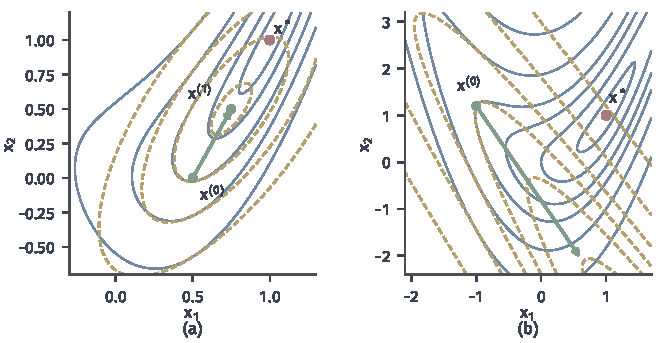
\includegraphics[width=112mm]{figures/05-optimization/02-smooth-optimization/matplotlib/newton-model-trust/figure.pdf}
  \caption{式~\eqref{eq:newton-running-objective}的等高线（蓝）与局部模型的等高线（黄色虚线）。(a)在$(\tfrac12,0)$处模型贴合良好，绿色箭头是Newton步，它的终点$\bm{x}^{(1)}$是模型的极小点。(b)在$(-1,\tfrac65)$处模型是一条几乎平直的长沟，绿色箭头按实际长度的$0.16$倍绘制，模型极小点$(9,-19)$在图外。两图中红点都是$\bm{x}^\star$。}
  \label{fig:newton-model-trust}
\end{BookInlineFigure}

\paragraph{可逆与正定各管什么}
方程~\eqref{eq:newton-equation}有唯一解只要求$\bm{H}^{(t)}$可逆；这个解是模型的极小点、并且指向下坡，要求的是正定。下面的结论把这两件事分开。

\begin{lemma}[正定曲率下的Newton方向]
\label{lem:newton-spd-direction}
设$\bm{H}^{(t)}\succ\bm{0}$，$\bm{g}^{(t)}\neq\bm{0}$。则$\bm{d}^{(t)}=-(\bm{H}^{(t)})^{-1}\bm{g}^{(t)}$是模型~\eqref{eq:newton-model}的唯一极小点，且满足
\begin{equation}
 (\bm{g}^{(t)})^\top\bm{d}^{(t)}=-(\bm{g}^{(t)})^\top(\bm{H}^{(t)})^{-1}\bm{g}^{(t)}<0.
 \label{eq:newton-descent}
\end{equation}
\end{lemma}

\begin{proof}
省略上标。任取位移$\bm{d}$，写成$\bm{d}=\bm{d}^{(t)}+\bm{w}$代入模型。一次项中用$\bm{g}=-\bm{H}\bm{d}^{(t)}$，含$\bm{w}$的一次项互相抵消，得到
\[
 m(\bm{d})=m(\bm{d}^{(t)})+\frac12\bm{w}^\top\bm{H}\bm{w}.
\]
$\bm{H}$正定，所以$\bm{w}\neq\bm{0}$时第二项严格为正，$\bm{d}^{(t)}$是唯一极小点。

下降性由定义代入得到。$\bm{H}$正定时$\bm{H}^{-1}$也正定，而$\bm{g}\neq\bm{0}$，于是二次型$\bm{g}^\top\bm{H}^{-1}\bm{g}$严格为正。
\end{proof}

图~\ref{fig:newton-curvature-cases}用三种曲率说明不正定时会发生什么。图(a)的$\bm{H}$正定，等高线是椭圆，方程的解是碗底。图(b)的$\bm{H}$可逆但不定，方程仍有唯一解，那个点却是马鞍的中心，模型沿某些方向可以无限下降，“走到模型的底”这句话失去了意义。图(c)的$\bm{H}$奇异，且$\bm{g}$不在它的值域内，方程无解，模型沿平坦方向一直倾斜。

\begin{BookInlineFigure}
  \centering
  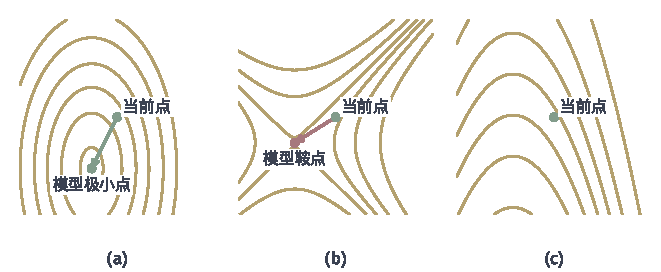
\includegraphics[width=112mm]{figures/05-optimization/02-smooth-optimization/matplotlib/newton-curvature-cases/figure.pdf}
  \caption{三种曲率下的局部模型，黄线为$m(\bm{d})$的等高线，绿色圆点是当前点。(a)$\bm{H}=\operatorname{diag}(2,0.6)$正定，Newton方程的解是模型的极小点。(b)$\bm{H}=\operatorname{diag}(1,-1)$不定，方程的解是模型的鞍点，用红色标出。(c)$\bm{H}=\operatorname{diag}(1,0)$奇异，$\bm{g}=(0.8,0.5)$不在值域内，方程无解。}
  \label{fig:newton-curvature-cases}
\end{BookInlineFigure}

在例子中可以看到“不定”的具体后果。取$\bm{x}=(0,\tfrac12)$，此时$u=\tfrac12$，$1-4u=-1<0$。由式~\eqref{eq:newton-running-derivatives}，
\[
 \bm{g}=\begin{bmatrix}-1\\1\end{bmatrix},\qquad
 \bm{H}=\begin{bmatrix}-1&0\\0&2\end{bmatrix}.
\]
由式~\eqref{eq:newton-running-direction}，Newton方向是$\bm{d}=(-1,-\tfrac12)$。方向导数为
\[
 \bm{g}^\top\bm{d}=1-\tfrac12=\tfrac12>0,
\]
所以这是一个上坡方向。走满一步到$(-1,0)$，目标从$0.75$升到$3$。

下表把三种情形并排。

\begin{BookInlineTable}
  \centering
  \begin{tabular}{@{}llll@{}}
    \toprule
    $\bm{H}^{(t)}$ & 方程~\eqref{eq:newton-equation} & 解的含义 & 方向 \\
    \midrule
    正定 & 唯一解 & 模型的唯一极小点 & 下降 \\
    可逆但不定 & 唯一解 & 模型的鞍点 & 可升可降 \\
    奇异 & 无解或无穷多解 & 无极小点或极小点不唯一 & 须另行处理 \\
    \bottomrule
  \end{tabular}
  \caption{曲率矩阵的性质与Newton方程的解。可逆只回答方程能否解，正定才回答解是否有用。}
  \label{tab:newton-curvature-cases}
\end{BookInlineTable}

\paragraph{不受坐标伸缩的影响}
Newton方向还有一个梯度方向没有的性质。第~\ref{chap:first-order-methods}章的方法在病态目标上吃亏，原因是步子的大小和各方向的弯度不匹配。Newton方向把弯度算进去了，因此和坐标的单位无关，就像一段路程不会因为改用千米记录而变长。

设$\bm{A}$是可逆矩阵，令$\bm{y}=\bm{A}\bm{x}$，$\tilde f(\bm{y})=f(\bm{A}^{-1}\bm{y})$。由链式法则，新坐标下的梯度和Hessian是
\[
 \nabla\tilde f=\bm{A}^{-\top}\bm{g},\qquad \nabla^2\tilde f=\bm{A}^{-\top}\bm{H}\bm{A}^{-1}.
\]
代入Newton方程，$\bm{A}^{-\top}$互相抵消，新坐标下的方向是
\[
 \tilde{\bm{d}}=-\bm{A}\bm{H}^{-1}\bm{A}^{\top}\bm{A}^{-\top}\bm{g}=\bm{A}\bm{d}.
\]
所以$\tilde{\bm{d}}$恰好是原方向$\bm{d}$在新坐标下的样子，整条迭代序列只是被$\bm{A}$映到了新坐标，这称为\term{仿射不变性}（affine invariance）。

负梯度方向不同。新坐标下它是$-\bm{A}^{-\top}\bm{g}$，而把原方向$-\bm{g}$映过去是$-\bm{A}\bm{g}$，两者只在$\bm{A}$为正交矩阵的倍数时平行。

图~\ref{fig:newton-affine}以$f(\bm{x})=\tfrac12(x_1^2+25x_2^2)$为例，条件数是$25$。Newton方向$\bm{d}=-\bm{H}^{-1}\bm{H}\bm{x}=-\bm{x}$，从任何起点都一步到达最小点，这对任意正定二次目标都成立。使用精确线搜索的梯度下降在原坐标下往复前进；换坐标$y_2=5x_2$后，等高线成了圆，两种方法才走同一条路。

\begin{BookInlineFigure}
  \centering
  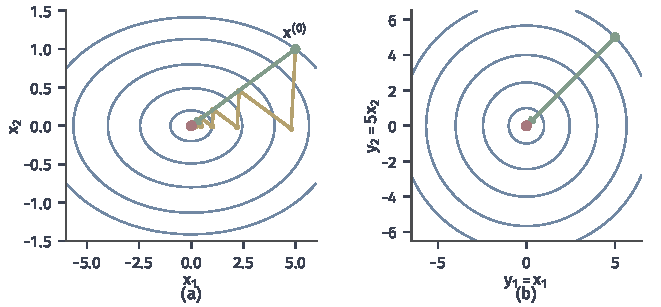
\includegraphics[width=112mm]{figures/05-optimization/02-smooth-optimization/matplotlib/newton-affine/figure.pdf}
  \caption{坐标变换对两种方向的影响，目标$\tfrac12(x_1^2+25x_2^2)$。(a)原坐标，从$(5,1)$出发，黄色折线是精确线搜索的梯度下降，绿色箭头是Newton步，红点是最小点。(b)取$y_2=5x_2$后等高线为圆，负梯度方向和Newton方向重合。Newton步在两张图中是同一步，只是用不同坐标表示。}
  \label{fig:newton-affine}
\end{BookInlineFigure}

仿射不变性说的是精确算术下的迭代。实际解方程时，$\bm{H}^{(t)}$的条件数仍然影响舍入误差，只是它不再决定迭代步数。

\paragraph{计算过程}
Newton法的公式已经由式~\eqref{eq:newton-equation}、\eqref{eq:newton-update}给出。下面用目标~\eqref{eq:newton-running-objective}从$(\tfrac12,0)$出发走一遍。这一节假定每个迭代点的Hessian都正定；不正定的情形由第~\ref{sec:newton-modified}节处理。

\needspace{6\baselineskip}
\paragraph{变量}
\begin{itemize}
 \item $\bm{x}\in\mathbb{R}^n$：当前点$\bm{x}^{(t)}$，在原处更新。
 \item $\bm{g}\in\mathbb{R}^n$：当前梯度。
 \item $\bm{H}\in\mathbb{R}^{n\times n}$：当前Hessian，对称。
 \item $\bm{L}\in\mathbb{R}^{n\times n}$：下三角矩阵，$\bm{H}$的Cholesky因子。
 \item $\bm{d}\in\mathbb{R}^n$：Newton方向。
 \item $\varepsilon>0$：梯度容差。
\end{itemize}

\paragraph{初始化}
选定初始点$\bm{x}^{(0)}$和容差$\varepsilon$，令$t=0$。例中初始点和容差为
\[
 \bm{x}^{(0)}=\bigl(\tfrac12,0\bigr),\qquad \varepsilon=10^{-6}.
\]

\needspace{6\baselineskip}
\paragraph{每轮更新}
在第$t$轮：
\begin{enumerate}
 \item \textbf{读取导数并检查停止。}计算$\bm{g}^{(t)}$和$\bm{H}^{(t)}$。若$\lVert\bm{g}^{(t)}\rVert_2\leq\varepsilon$，输出$\bm{x}^{(t)}$并结束。

 例中第一轮$u=-\tfrac14$，由式~\eqref{eq:newton-running-derivatives}，
 \[
  \bm{g}^{(0)}=\begin{bmatrix}0\\-\tfrac12\end{bmatrix},\qquad
  \bm{H}^{(0)}=\begin{bmatrix}4&-2\\-2&2\end{bmatrix}.
 \]

 \item \textbf{分解。}计算Cholesky分解$\bm{H}^{(t)}=\bm{L}\bm{L}^\top$。

 例中第一轮
 \[
  \bm{L}=\begin{bmatrix}2&0\\-1&1\end{bmatrix}.
 \]

 \item \textbf{回代求方向。}先由前代解$\bm{L}\bm{y}=-\bm{g}^{(t)}$，再由回代解$\bm{L}^\top\bm{d}^{(t)}=\bm{y}$。

 例中第一轮的中间向量和方向分别是
 \[
  \bm{y}=\begin{bmatrix}0\\\tfrac12\end{bmatrix},\qquad
  \bm{d}^{(0)}=\begin{bmatrix}\tfrac14\\\tfrac12\end{bmatrix}.
 \]

 \item \textbf{更新。}按式~\eqref{eq:newton-update}走到下一点，令$t\leftarrow t+1$。

 例中第一轮到达$\bm{x}^{(1)}=(\tfrac34,\tfrac12)$，目标从$\tfrac3{16}$降到$\tfrac9{256}\approx0.0352$。

 第二轮$u=\tfrac12-\tfrac9{16}=-\tfrac1{16}$。这时用手解直接套式~\eqref{eq:newton-running-direction}更快：
 \[
  d_1=\frac{1/4}{1+1/4}=\frac15,\qquad
  d_2=\frac1{16}+\frac32\cdot\frac15=0.3625.
 \]
 于是$\bm{x}^{(2)}=(0.95,0.8625)$，目标降到$0.00285$。
\end{enumerate}

各轮结果列在表~\ref{tab:newton-pure-run}中。第$5$轮梯度范数已低于容差，迭代结束，最终得到$\bm{x}^{(5)}\approx(1,1)$，与解的距离约$2.4\times10^{-8}$。图~\ref{fig:newton-path}画出了前几步的路径。

\begin{BookInlineTable}
  \centering
  \small
  \begin{tabular}{@{}cccccc@{}}
    \toprule
    $t$ & $\bm{x}^{(t)}$ & $f$ & $\lVert\bm{g}^{(t)}\rVert_2$ & $\bm{d}^{(t)}$ & $\lVert\bm{x}^{(t)}-\bm{x}^\star\rVert_2$ \\
    \midrule
    $0$ & $(0.5,0)$ & $0.1875$ & $0.5$ & $(0.25,0.5)$ & $1.118$ \\
    $1$ & $(0.75,0.5)$ & $0.03516$ & $0.1398$ & $(0.2,0.3625)$ & $0.5590$ \\
    $2$ & $(0.95,0.8625)$ & $2.85\mathrm{e}{-3}$ & $0.1296$ & $(0.0431,0.1219)$ & $0.1463$ \\
    $3$ & $(0.9931,0.9844)$ & $2.72\mathrm{e}{-5}$ & $3.75\mathrm{e}{-3}$ & $(0.0068,0.0155)$ & $0.01706$ \\
    $4$ & $(0.99995,0.99985)$ & $3.49\mathrm{e}{-9}$ & $1.66\mathrm{e}{-4}$ & $(5\mathrm{e}{-5},1.5\mathrm{e}{-4})$ & $1.57\mathrm{e}{-4}$ \\
    $5$ & $(1.0000,1.0000)$ & $5.2\mathrm{e}{-17}$ & $5.2\mathrm{e}{-9}$ & 停止 & $2.4\mathrm{e}{-8}$ \\
    \bottomrule
  \end{tabular}
  \caption{Newton法在目标~\eqref{eq:newton-running-objective}上从$(\tfrac12,0)$出发的迭代。第$3$行以后，误差每步大约平方一次。}
  \label{tab:newton-pure-run}
\end{BookInlineTable}

\begin{BookInlineFigure}
  \centering
  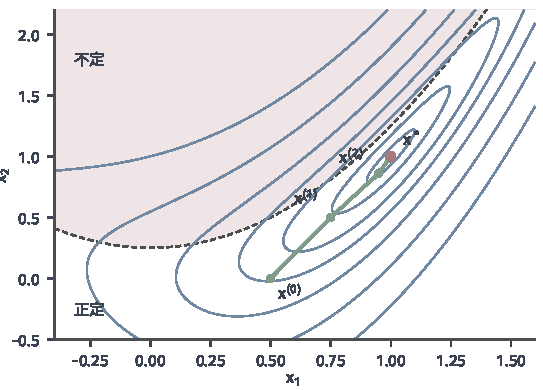
\includegraphics[width=92mm]{figures/05-optimization/02-smooth-optimization/matplotlib/newton-path/figure.pdf}
  \caption{Newton法的迭代路径（绿）。蓝线是目标~\eqref{eq:newton-running-objective}的等高线，红色浅底是Hessian不定的区域，深灰色虚线是它的边界$x_2=x_1^2+\tfrac14$，红点是解。起点$(\tfrac12,0)$在正定区域内，路径紧贴山谷前进，始终没有进入浅底区域。}
  \label{fig:newton-path}
\end{BookInlineFigure}

路径始终在正定区域内，这一点在本例中可以验证。整步之后的$u$值为
\[
 u^{+}=(x_2+d_2)-(x_1+d_1)^2=u+d_2-2x_1d_1-d_1^2.
\]
代入式~\eqref{eq:newton-running-direction}的$d_2$，前三项相消，得到
\[
 u^{+}=-d_1^2\leq0.
\]
因此任意一个完整Newton步之后都有$1-4u^+\geq1>0$。这是此目标特有的结构，一般目标没有这样的保证。

\paragraph{局部二次收敛}
表~\ref{tab:newton-pure-run}最后几行显示，误差接近解时每步大约平方一次。下面说明这种现象来自哪里。先从直观上看：在解附近，目标和它的二次模型只差三阶小量；二次模型的极小点又恰好由Newton步算出，所以Newton步的误差只由这个三阶差决定，比一阶方法“每步打一个固定折扣”好得多。

称一列点\term{二次收敛}（quadratic convergence）到$\bm{x}^\star$，如果存在常数$C$，使充分大的$t$都满足
\begin{equation}
 \lVert\bm{x}^{(t+1)}-\bm{x}^\star\rVert_2\leq C\lVert\bm{x}^{(t)}-\bm{x}^\star\rVert_2^2.
 \label{eq:newton-quadratic-definition}
\end{equation}
定理需要在解附近控制Hessian，记$\mu$为解处Hessian的最小特征值，$M$为Hessian的Lipschitz常数。

\begin{theorem}[Newton法的局部二次收敛]
\label{thm:newton-local}
设$f$在以$\bm{x}^\star$为中心、半径为$r$的开球$\bm{B}$上二阶连续可微，$\nabla f(\bm{x}^\star)=\bm{0}$，$\nabla^2f(\bm{x}^\star)\succeq\mu\bm{I}$，其中$\mu>0$，并且对$\bm{x},\bm{y}\in\bm{B}$有
\begin{equation}
 \lVert\nabla^2f(\bm{x})-\nabla^2f(\bm{y})\rVert_2\leq M\lVert\bm{x}-\bm{y}\rVert_2.
 \label{eq:newton-hessian-lipschitz}
\end{equation}
记$\rho=\min\{r,\ \mu/(2M)\}$。若$\lVert\bm{x}^{(t)}-\bm{x}^\star\rVert_2<\rho$，则$\bm{H}^{(t)}\succeq\tfrac\mu2\bm{I}$，Newton步有定义，且
\begin{equation}
 \lVert\bm{x}^{(t+1)}-\bm{x}^\star\rVert_2\leq\frac{M}{\mu}\lVert\bm{x}^{(t)}-\bm{x}^\star\rVert_2^2.
 \label{eq:newton-quadratic-bound}
\end{equation}
因此，只要$\lVert\bm{x}^{(0)}-\bm{x}^\star\rVert_2<\rho$，所有迭代点都留在半径$\rho$的球内，并且
\begin{equation}
 \frac{M}{\mu}\lVert\bm{x}^{(t)}-\bm{x}^\star\rVert_2\leq\Bigl(\frac12\Bigr)^{2^t}.
 \label{eq:newton-doubly-exponential}
\end{equation}
\end{theorem}

\begin{proof}
记$\bm{e}=\bm{x}^{(t)}-\bm{x}^\star$，$\bm{H}=\bm{H}^{(t)}$，并设$\lVert\bm{e}\rVert_2<\rho$。

第一步说明$\bm{H}$的逆有界。由式~\eqref{eq:newton-hessian-lipschitz}，
\[
 \lVert\bm{H}-\nabla^2f(\bm{x}^\star)\rVert_2\leq M\lVert\bm{e}\rVert_2\leq\frac\mu2.
\]
对称矩阵的特征值受扰动量控制，所以$\lambda_{\min}(\bm{H})\geq\mu-\mu/2$，即
\[
 \bm{H}\succeq\frac\mu2\bm{I},\qquad \lVert\bm{H}^{-1}\rVert_2\leq\frac2\mu.
\]

第二步写出误差的递推。由$\nabla f(\bm{x}^\star)=\bm{0}$，沿线段积分，
\[
 \bm{g}^{(t)}=\int_0^1\nabla^2f(\bm{x}^\star+s\bm{e})\bm{e}\,\mathrm{d}s.
\]
Newton步之后的误差是$\bm{e}-\bm{H}^{-1}\bm{g}^{(t)}$。把$\bm{e}$写成$\bm{H}^{-1}\bm{H}\bm{e}$并合并，得到
\[
 \bm{x}^{(t+1)}-\bm{x}^\star=\bm{H}^{-1}\int_0^1\bigl(\bm{H}-\nabla^2f(\bm{x}^\star+s\bm{e})\bigr)\bm{e}\,\mathrm{d}s.
\]

第三步估计积分。点$\bm{x}^{(t)}$与$\bm{x}^\star+s\bm{e}$相距$(1-s)\lVert\bm{e}\rVert_2$，由式~\eqref{eq:newton-hessian-lipschitz}，
\[
 \Bigl\lVert\int_0^1\bigl(\bm{H}-\nabla^2f(\bm{x}^\star+s\bm{e})\bigr)\bm{e}\,\mathrm{d}s\Bigr\rVert_2
 \leq\int_0^1M(1-s)\lVert\bm{e}\rVert_2^2\,\mathrm{d}s=\frac M2\lVert\bm{e}\rVert_2^2.
\]
与第一步的$2/\mu$相乘，即得式~\eqref{eq:newton-quadratic-bound}。

最后讨论序列。记
\[
 a_t=\frac M\mu\lVert\bm{x}^{(t)}-\bm{x}^\star\rVert_2,
\]
式~\eqref{eq:newton-quadratic-bound}写成$a_{t+1}\leq a_t^2$。由初始距离小于$\rho\leq\mu/(2M)$得$a_0<\tfrac12$。于是误差每步至少减半，迭代点不离开球，归纳得$a_t\leq a_0^{2^t}\leq(\tfrac12)^{2^t}$。
\end{proof}

式~\eqref{eq:newton-doubly-exponential}说明，进入这个邻域后，有效数字大约每步翻倍。回到$f(x)=e^x-2x$，从$1.5$出发的误差依次是
\[
 0.807,\quad 0.253,\quad 0.0295,\quad 4.31\times10^{-4},\quad 9.27\times10^{-8},\quad 4.33\times10^{-15}.
\]
相邻两步的比值$e^{(t+1)}/(e^{(t)})^2$依次约为
\[
 0.39,\quad 0.46,\quad 0.50,\quad 0.50,\quad 0.50,
\]
趋于$f'''(x^\star)/(2f''(x^\star))=\tfrac12$。

对主例~\eqref{eq:newton-running-objective}，解处Hessian的特征值约为$0.185$和$10.8$，所以$\mu\approx0.185$；在解附近数值估计$M\approx25$，定理保证的半径$\mu/(2M)$只有约$0.0037$。表~\ref{tab:newton-pure-run}的迭代却从距离$1.1$处就进展顺利。定理给出的是充分条件，半径通常十分保守；它的价值在于说明快速收敛的机制和所需的条件。

图~\ref{fig:newton-order}(a)比较了同一起点上的Newton法和使用回溯线搜索的梯度下降，后者的步长规则由下一节的式~\eqref{eq:newton-armijo}规定。解处的条件数约为$58$，梯度下降要$245$步才能把梯度范数降到$10^{-6}$，Newton法用了$5$步。

\begin{BookInlineFigure}
  \centering
  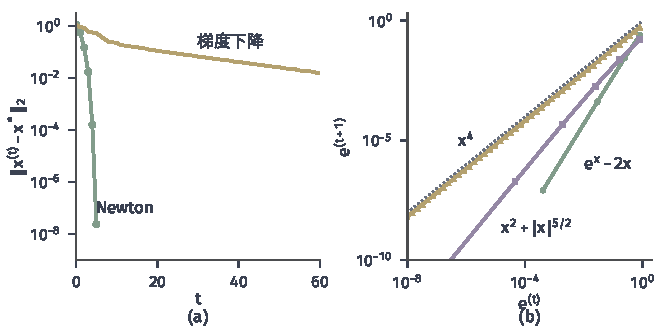
\includegraphics[width=112mm]{figures/05-optimization/02-smooth-optimization/matplotlib/newton-order/figure.pdf}
  \caption{收敛阶的比较。(a)目标~\eqref{eq:newton-running-objective}上从$(\tfrac12,0)$出发的距离误差，绿线为Newton法，黄线为回溯梯度下降。(b)双对数坐标下相邻两步一维误差的关系：绿线$e^x-2x$斜率约为$2$，紫线$x^2+\lvert x\rvert^{5/2}$斜率约为$1.5$，黄线$x^4$斜率为$1$且接近灰色虚线$e^{(t+1)}=e^{(t)}$。}
  \label{fig:newton-order}
\end{BookInlineFigure}

\paragraph{三个条件的作用}
定理有三个条件：解处Hessian正定、Hessian Lipschitz连续、初始点足够近。逐一去掉，可以看到结论怎样变弱。

去掉解处正定，看$f(x)=x^4$。解是$0$，但$f''(0)=0$，这是退化的极小点。Newton更新为
\[
 x^{(t+1)}=x^{(t)}-\frac{4(x^{(t)})^3}{12(x^{(t)})^2}=\frac23x^{(t)}.
\]
收敛只是线性的，误差每步乘以固定的$\tfrac23$。式~\eqref{eq:newton-quadratic-bound}中的$M/\mu$此时为无穷大，模型的底沿平坦方向已不再贴近真解。

去掉Hessian的Lipschitz连续，看$f(x)=x^2+\lvert x\rvert^{5/2}$。它的解是$0$，$f''(0)=2$，但$f''$在$0$处只是$\tfrac12$阶Hölder连续。对$x>0$，
\[
 f'(x)=2x+\tfrac52x^{3/2},\qquad f''(x)=2+\tfrac{15}4x^{1/2}.
\]
代入Newton更新并通分，分子中的一次项抵消，得到
\[
 x^{(t+1)}=\frac{\frac54(x^{(t)})^{3/2}}{2+\frac{15}4(x^{(t)})^{1/2}}\approx\frac58(x^{(t)})^{3/2}.
\]
误差的阶从$2$降为$\tfrac32$，仍快于线性，但不再是二次。图~\ref{fig:newton-order}(b)中三条线的斜率正是收敛阶。

去掉初始点足够近，看严格凸函数$\varphi(x)=\sqrt{1+x^2}$。求导得
\[
 \varphi'(x)=\frac{x}{\sqrt{1+x^2}},\qquad \varphi''(x)=(1+x^2)^{-3/2}.
\]
代入Newton更新，得到极简的递推
\begin{equation}
 x^{(t+1)}=x^{(t)}-x^{(t)}\bigl(1+(x^{(t)})^2\bigr)=-(x^{(t)})^3.
 \label{eq:newton-cubic-map}
\end{equation}
$\lvert x^{(0)}\rvert<1$时迭代收敛，$\lvert x^{(0)}\rvert=1$时在$\pm1$之间来回跳，$\lvert x^{(0)}\rvert>1$时发散。图~\ref{fig:newton-basin}(a)说明了原因：$x$很大时函数几乎是直线，曲率很小，模型的底在非常远的地方。这个函数处处解析、处处严格凸，Newton法照样发散，所以局部定理中的“足够近”不能省略。

\begin{BookInlineFigure}
  \centering
  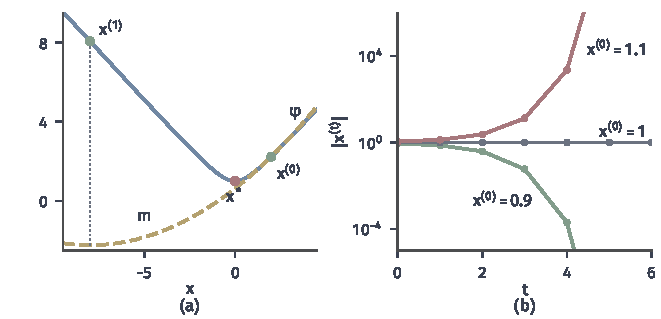
\includegraphics[width=112mm]{figures/05-optimization/02-smooth-optimization/matplotlib/newton-basin/figure.pdf}
  \caption{严格凸函数$\varphi(x)=\sqrt{1+x^2}$上Newton法的局部性。(a)蓝线是$\varphi$，黄色虚线是$x^{(0)}=2$处的二次模型，模型的底在$x=-8$，绿点标出实际到达的新点，$\varphi$反而升高。(b)递推$x^{(t+1)}=-(x^{(t)})^3$的三条轨迹，纵轴为绝对值，初值分别为$0.9$（绿）、$1$（灰）、$1.1$（红）。}
  \label{fig:newton-basin}
\end{BookInlineFigure}

\section{阻尼Newton法}
\label{sec:newton-damped}

上一节的定理只管解附近。接下来要弄清：Hessian仍然正定，但当前点离解很远，模型的底不可信，怎样在不改变方向的前提下保证目标确实下降，又不损失解附近的快速收敛？

\paragraph{完整Newton步的麻烦}
回到目标~\eqref{eq:newton-running-objective}，从$\bm{x}^{(0)}=(-1,\tfrac65)$出发。此处$u=\tfrac15$，Hessian的行列式是$2(1-4u)=0.4$，正定但接近奇异。由式~\eqref{eq:newton-running-direction}，
\[
 d_1=\frac{2}{0.2}=10,\qquad d_2=-\frac15-2\cdot10=-20.2.
\]
走满一步到达$(9,-19)$，目标从$2.04$升到$10032$。

Newton方向在这里是下降方向，毛病出在走得太远。按式~\eqref{eq:newton-running-direction}继续走完整步，迭代点在$(9,-19)$、$(8.98,80.6)$、$(1.01,-62.5)$之间大幅跳动，几步之后才落回解附近，见图~\ref{fig:newton-damped-path}(a)。这条路径能回来，靠的是上一节提到的此目标的特殊结构。一般目标没有这种运气，式~\eqref{eq:newton-cubic-map}的发散就是例子。

\paragraph{主要思想}
Newton方向是模型认为最好的方向，模型的问题主要在于它在远处高估了自己。一个自然的补救是保留方向，但只走其中的一段，走多少由原目标来核验：
\begin{equation}
 \bm{x}^{(t+1)}=\bm{x}^{(t)}+\alpha^{(t)}\bm{d}^{(t)},\qquad 0<\alpha^{(t)}\leq1.
 \label{eq:newton-damped-update}
\end{equation}
这称为\term{阻尼Newton法}（damped Newton method）。方向仍由方程~\eqref{eq:newton-equation}确定，改变的只是这一步信模型信到什么程度。

核验用第~\ref{chap:smooth-foundations}章的Armijo条件。给定$c\in(0,\tfrac12)$，要求实际下降至少达到一阶预测的$c$倍：
\begin{equation}
 f(\bm{x}^{(t)}+\alpha\bm{d}^{(t)})\leq f(\bm{x}^{(t)})+c\,\alpha\,(\bm{g}^{(t)})^\top\bm{d}^{(t)}.
 \label{eq:newton-armijo}
\end{equation}
回溯的做法是先试$\alpha=1$，不满足就乘以$\beta\in(0,1)$，直到满足为止。上限取$1$、并且先试$1$，理由在本节后面说明。

方向导数$(\bm{g}^{(t)})^\top\bm{d}^{(t)}$在这里有专门的意义。记
\begin{equation}
 (\omega^{(t)})^2=-(\bm{g}^{(t)})^\top\bm{d}^{(t)}=(\bm{g}^{(t)})^\top(\bm{H}^{(t)})^{-1}\bm{g}^{(t)}.
 \label{eq:newton-decrement}
\end{equation}
$\omega^{(t)}$称为\term{Newton减量}（Newton decrement）。把$\bm{d}^{(t)}$代入模型，再用$\bm{H}^{(t)}\bm{d}^{(t)}=-\bm{g}^{(t)}$，得到模型的预测下降量
\[
 m^{(t)}(\bm{0})-m^{(t)}(\bm{d}^{(t)})=\frac12(\omega^{(t)})^2.
\]
所以$\tfrac12(\omega^{(t)})^2$是模型对“还能下降多少”的估计，可以作为停止标准。它和Newton方向一样不受坐标伸缩影响，梯度范数则没有这种性质。

\paragraph{正定性为回溯提供了什么}
回溯要能结束，当前方向必须是下降方向。由式~\eqref{eq:newton-descent}，$\bm{H}^{(t)}\succ\bm{0}$时$(\omega^{(t)})^2>0$。把目标限制在这个方向上，记一元函数$\varphi(\alpha)$为沿方向走$\alpha$时的目标值，它在$0$处的导数是$-(\omega^{(t)})^2<0$，于是
\[
 \varphi(\alpha)=\varphi(0)-\alpha(\omega^{(t)})^2+o(\alpha).
\]
由于$c<1$，当$\alpha$足够小时，式~\eqref{eq:newton-armijo}成立，回溯在有限次内结束。

如果$\bm{H}^{(t)}$不定，这个保证就没有了。第~\ref{sec:newton-basic}节的点$(0,\tfrac12)$处方向导数为$\tfrac12>0$，式~\eqref{eq:newton-armijo}的右端随$\alpha$增大而升高，而左端在小$\alpha$上升得比右端更快，因为$c<1$。无论$\alpha$多小都不满足，回溯永远停不下来。阻尼只能调整走多远，不能把上坡的方向变成下坡。

\paragraph{计算过程}
仍用目标~\eqref{eq:newton-running-objective}，从上面的坏起点$(-1,\tfrac65)$出发。

\needspace{6\baselineskip}
\paragraph{变量}
\begin{itemize}
 \item $\bm{x},\bm{g},\bm{H},\bm{d}$：与Newton法相同，分别是当前点、梯度、Hessian和Newton方向。
 \item $\omega^2$：Newton减量的平方，同时是方向导数的相反数。
 \item $\alpha$：当前试探步长，每轮从$1$开始。
 \item $c,\beta$：Armijo参数和回溯因子，全程固定。
 \item $\varepsilon$：停止容差，判断$\tfrac12\omega^2\leq\varepsilon$。
\end{itemize}

\paragraph{初始化}
选定$\bm{x}^{(0)}$，$c\in(0,\tfrac12)$，$\beta\in(0,1)$，$\varepsilon>0$。例中取下面的数据：
\[
 \bm{x}^{(0)}=\bigl(-1,\tfrac65\bigr),\qquad c=0.1,\qquad \beta=0.5,\qquad \varepsilon=10^{-10}.
\]

\needspace{6\baselineskip}
\paragraph{每轮更新}
在第$t$轮：
\begin{enumerate}
 \item \textbf{求Newton方向。}计算$\bm{g}^{(t)}$、$\bm{H}^{(t)}$，用Cholesky分解解方程~\eqref{eq:newton-equation}。

 例中第一轮
 \[
  \bm{g}^{(0)}=\begin{bmatrix}-1.2\\0.4\end{bmatrix},\qquad
  \bm{H}^{(0)}=\begin{bmatrix}8.2&4\\4&2\end{bmatrix},\qquad
  \bm{d}^{(0)}=\begin{bmatrix}10\\-20.2\end{bmatrix}.
 \]

 \item \textbf{检查停止。}按式~\eqref{eq:newton-decrement}计算$\omega^2$。若$\tfrac12\omega^2\leq\varepsilon$，输出$\bm{x}^{(t)}$并结束。

 例中第一轮
 \[
  (\omega^{(0)})^2=12+8.08=20.08.
 \]

 \item \textbf{回溯。}令$\alpha=1$。当式~\eqref{eq:newton-armijo}不成立时，令$\alpha\leftarrow\beta\alpha$。

 例中第一轮的右端是$2.04-2.008\alpha$，试探结果如下：
 \[
  \begin{array}{ccccc}
   \alpha&1&1/2&1/4&1/8\\
   f(\bm{x}^{(0)}+\alpha\bm{d}^{(0)})&10032&624.5&37.34&2.206\\
   \text{右端}&0.032&1.036&1.538&1.789
  \end{array}
 \]
 四次都被拒绝。下一次试探$\alpha=\tfrac1{16}$，新点是$(-0.375,-0.0625)$，目标值$0.9866$，右端$1.9145$，条件满足，接受。

 \item \textbf{更新。}按式~\eqref{eq:newton-damped-update}走到下一点，令$t\leftarrow t+1$。

 例中第一轮到达$\bm{x}^{(1)}=(-0.375,-0.0625)$。

 第二轮$u=-0.203125$，由式~\eqref{eq:newton-running-derivatives}和式~\eqref{eq:newton-running-direction}，
 \[
  \bm{g}^{(1)}=\begin{bmatrix}-1.6797\\-0.4063\end{bmatrix},\qquad
  \bm{d}^{(1)}=\begin{bmatrix}0.7586\\-0.3658\end{bmatrix},\qquad
  (\omega^{(1)})^2=1.1256.
 \]
 试探$\alpha=1$，新点的目标值是$0.5212$，右端是$0.9866-0.1126=0.8740$，第一次试探即被接受。
\end{enumerate}

图~\ref{fig:newton-backtrack}是第一轮回溯的情形。表~\ref{tab:newton-damped-run}列出各轮结果。第$1$轮以后每次都是$\alpha=1$第一次就被接受。第$7$轮$\tfrac12\omega^2$已低于容差，迭代结束，最终得到$\bm{x}^{(7)}\approx(1,1)$，目标值约$7.6\times10^{-15}$。

\begin{BookInlineFigure}
  \centering
  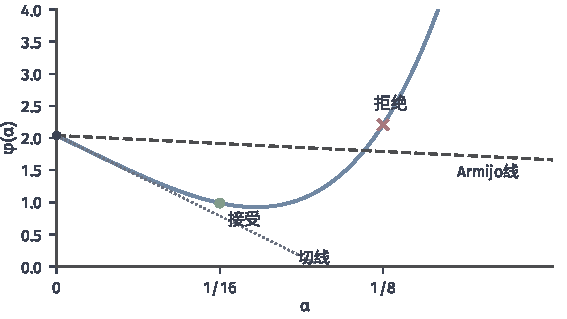
\includegraphics[width=96mm]{figures/05-optimization/02-smooth-optimization/matplotlib/newton-backtrack/figure.pdf}
  \caption{第一轮回溯沿方向的一元函数$\varphi(\alpha)=f(\bm{x}^{(0)}+\alpha\bm{d}^{(0)})$（蓝）。灰色点线是$\alpha=0$处的切线，深灰色虚线是Armijo线$\varphi(0)+c\alpha\varphi'(0)$，曲线在Armijo线下方的步长才可接受。$\alpha=\tfrac18$处（红叉）目标在线上方，被拒绝；$\alpha=\tfrac1{16}$处（绿点）被接受。$\alpha=1,\tfrac12,\tfrac14$在图外，目标值更高。}
  \label{fig:newton-backtrack}
\end{BookInlineFigure}

\begin{BookInlineTable}
  \centering
  \begin{tabular}{@{}ccccc@{}}
    \toprule
    $t$ & $\bm{x}^{(t)}$ & $f$ & $(\omega^{(t)})^2$ & $\alpha^{(t)}$ \\
    \midrule
    $0$ & $(-1,1.2)$ & $2.04$ & $20.08$ & $1/16$ \\
    $1$ & $(-0.375,-0.0625)$ & $0.9866$ & $1.1256$ & $1$ \\
    $2$ & $(0.3836,-0.4283)$ & $0.5212$ & $0.7775$ & $1$ \\
    $3$ & $(0.5703,0.2904)$ & $0.09354$ & $0.1645$ & $1$ \\
    $4$ & $(0.9474,0.7554)$ & $0.02161$ & $0.04223$ & $1$ \\
    $5$ & $(0.9809,0.9611)$ & $1.83\mathrm{e}{-4}$ & $3.64\mathrm{e}{-4}$ & $1$ \\
    $6$ & $(0.99992,0.99947)$ & $1.33\mathrm{e}{-7}$ & $2.67\mathrm{e}{-7}$ & $1$ \\
    $7$ & $(1.0000,1.0000)$ & $7.6\mathrm{e}{-15}$ & $1.5\mathrm{e}{-14}$ & 停止 \\
    \bottomrule
  \end{tabular}
  \caption{阻尼Newton法从$(-1,\tfrac65)$出发的迭代，$c=0.1$，$\beta=0.5$。只有第一轮的方向需要缩短，其余各轮都接受完整步。}
  \label{tab:newton-damped-run}
\end{BookInlineTable}

\begin{BookInlineFigure}
  \centering
  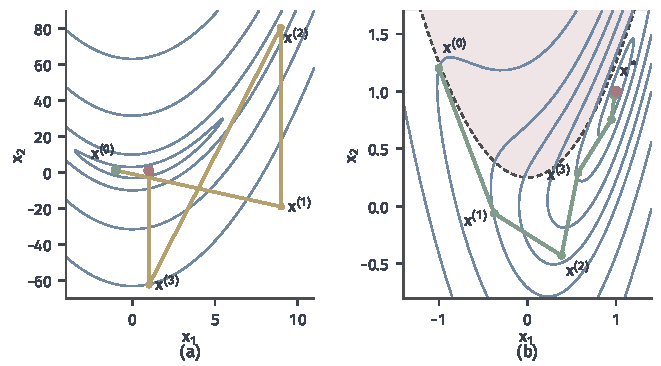
\includegraphics[width=112mm]{figures/05-optimization/02-smooth-optimization/matplotlib/newton-damped-path/figure.pdf}
  \caption{从$(-1,\tfrac65)$出发的两条路径，蓝线是等高线，红点是解。(a)完整Newton步（黄）在大范围内来回跳动，纵轴范围约$160$。(b)阻尼Newton法（绿）第一步只走$\tfrac1{16}$，随后沿山谷收敛，红色浅底是Hessian不定的区域。}
  \label{fig:newton-damped-path}
\end{BookInlineFigure}

图~\ref{fig:newton-damped-history}把目标值和步长画成曲线。完整Newton步的目标值先冲到$10^4$的量级，阻尼方法则严格逐步下降。值得注意的是，完整步的路径从第$4$轮起目标值反而更低，因为它恰好跳到了解附近；阻尼保证的是每一步可靠，并不保证每条路径的步数都最少。

\begin{BookInlineFigure}
  \centering
  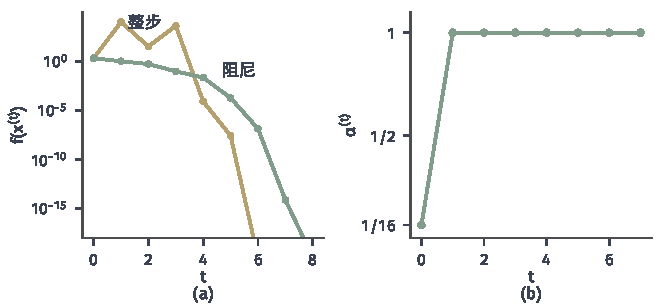
\includegraphics[width=112mm]{figures/05-optimization/02-smooth-optimization/matplotlib/newton-damped-history/figure.pdf}
  \caption{图~\ref{fig:newton-damped-path}两条路径的数值。(a)目标值的半对数曲线，绿线为阻尼Newton法，黄线为完整Newton步。(b)阻尼Newton法各轮接受的步长，第一轮之后都是$1$。}
  \label{fig:newton-damped-history}
\end{BookInlineFigure}

\paragraph{强凸目标上的全局收敛}
现在把“回溯总能带来足够下降”写成定理。定理需要曲率的上下界，用来保证方向既不太长也不太偏。假设对全空间成立是为了证明简洁；真正用到的只是初始下水平集附近的界，这时要额外说明所有试探点留在该区域内。

\begin{theorem}[阻尼Newton法的全局线性收敛]
\label{thm:newton-damped-global}
设$f$二阶连续可微，且对所有$\bm{x}$，$\mu\bm{I}\preceq\nabla^2f(\bm{x})\preceq L\bm{I}$，其中$0<\mu\leq L$，记$\kappa=L/\mu$。取$c\in(0,\tfrac12)$，$\beta\in(0,1)$。则回溯总在有限次内结束，接受的步长满足$\alpha^{(t)}\geq\beta/\kappa$，并且
\begin{equation}
 f(\bm{x}^{(t+1)})-f^\star\leq\Bigl(1-\frac{2c\beta}{\kappa^2}\Bigr)\bigl(f(\bm{x}^{(t)})-f^\star\bigr).
 \label{eq:newton-damped-linear}
\end{equation}
\end{theorem}

\begin{proof}
省略上标。第一步估计沿方向的上界。曲率上界$L$给出
\[
 f(\bm{x}+\alpha\bm{d})\leq f(\bm{x})+\alpha\bm{g}^\top\bm{d}+\frac L2\alpha^2\lVert\bm{d}\rVert_2^2.
\]
由式~\eqref{eq:newton-decrement}，$\bm{g}^\top\bm{d}=-\omega^2$。又由$\bm{H}\succeq\mu\bm{I}$，
\[
 \omega^2=\bm{d}^\top\bm{H}\bm{d}\geq\mu\lVert\bm{d}\rVert_2^2.
\]
代入上式，
\[
 f(\bm{x}+\alpha\bm{d})\leq f(\bm{x})-\alpha\omega^2+\frac\kappa2\alpha^2\omega^2.
\]

第二步确定可接受的步长范围。与式~\eqref{eq:newton-armijo}比较，只要$-1+\tfrac\kappa2\alpha\leq-c$，也就是$\alpha\leq2(1-c)/\kappa$，Armijo条件就成立。

第三步给出步长下界。若$\alpha=1$被接受，则$\alpha=1\geq\beta/\kappa$。否则上一个试探值$\alpha/\beta$被拒绝，必有$\alpha/\beta>2(1-c)/\kappa$。由$c<\tfrac12$得$2(1-c)>1$，所以$\alpha>\beta/\kappa$。

第四步估计下降量。由式~\eqref{eq:newton-armijo}和步长下界，
\[
 f(\bm{x})-f(\bm{x}^{(t+1)})\geq c\alpha\omega^2\geq\frac{c\beta}\kappa\omega^2.
\]
由$\bm{H}^{-1}\succeq L^{-1}\bm{I}$，有$\omega^2\geq\lVert\bm{g}\rVert_2^2/L$。

第五步用梯度控制目标差。强凸性给出，对任意$\bm{y}$，
\[
 f(\bm{y})\geq f(\bm{x})+\bm{g}^\top(\bm{y}-\bm{x})+\frac\mu2\lVert\bm{y}-\bm{x}\rVert_2^2\geq f(\bm{x})-\frac{\lVert\bm{g}\rVert_2^2}{2\mu},
\]
其中第二个不等号是对$\bm{y}$取右端的最小值。令$\bm{y}=\bm{x}^\star$，得$\lVert\bm{g}\rVert_2^2\geq2\mu(f(\bm{x})-f^\star)$。

综合第四、第五步，
\[
 f(\bm{x})-f(\bm{x}^{(t+1)})\geq\frac{c\beta}{\kappa L}\cdot2\mu\bigl(f(\bm{x})-f^\star\bigr)=\frac{2c\beta}{\kappa^2}\bigl(f(\bm{x})-f^\star\bigr).
\]
两边减$f^\star$后整理，即得式~\eqref{eq:newton-damped-linear}。
\end{proof}

这个速率含$\kappa^2$，远比实际表现差，而且算法本身不受坐标伸缩的影响，界却依赖坐标下的$\mu,L$。定理的作用不在于预测步数，而在于保证从任何起点出发目标都稳定下降，梯度趋于零。要得到不依赖坐标的步数界，需要对三阶导数作更细致的假设，证明篇幅较长，读者可查阅\scite{math-boyd2004convex}。

\paragraph{完整步何时恢复}
全局定理保证迭代进入解的附近，但如果进入后步长仍小于$1$，局部二次收敛就得不到。表~\ref{tab:newton-damped-run}显示步长很快回到$1$，下面的定理说明这不是偶然。

\begin{theorem}[完整步的接受与二次收敛]
\label{thm:newton-unit-step}
在定理~\ref{thm:newton-damped-global}的条件下，再设$\nabla^2f$是$M$-Lipschitz的，记
\begin{equation}
 \tau=\min\bigl\{1,\,3(1-2c)\bigr\}\frac{\mu^2}{M}.
 \label{eq:newton-unit-threshold}
\end{equation}
若$\lVert\bm{g}^{(t)}\rVert_2\leq\tau$，则$\alpha=1$通过Armijo检验，且
\begin{equation}
 \lVert\bm{g}^{(t+1)}\rVert_2\leq\frac{M}{2\mu^2}\lVert\bm{g}^{(t)}\rVert_2^2\leq\frac12\lVert\bm{g}^{(t)}\rVert_2.
 \label{eq:newton-gradient-quadratic}
\end{equation}
因此一旦某轮梯度范数不超过$\tau$，此后每轮都接受完整步，梯度范数二次收敛到零。
\end{theorem}

\begin{proof}
省略上标。令$h(s)=f(\bm{x}+s\bm{d})$。先用Taylor公式的积分余项写出
\[
 h(1)=h(0)+h'(0)+\int_0^1(1-s)h''(s)\,\mathrm{d}s.
\]
这里$h'(0)=-\omega^2$。由Hessian的Lipschitz条件，
\[
 h''(s)=\bm{d}^\top\nabla^2f(\bm{x}+s\bm{d})\bm{d}\leq\omega^2+Ms\lVert\bm{d}\rVert_2^3.
\]
代入积分，得到
\[
 f(\bm{x}+\bm{d})\leq f(\bm{x})-\frac12\omega^2+\frac M6\lVert\bm{d}\rVert_2^3.
\]

要通过Armijo检验，只需
\[
 \frac M6\lVert\bm{d}\rVert_2^3\leq\Bigl(\frac12-c\Bigr)\omega^2.
\]
由$\lVert\bm{d}\rVert_2^2\leq\omega^2/\mu$，只需$\lVert\bm{d}\rVert_2\leq3(1-2c)\mu/M$。而$\lVert\bm{d}\rVert_2\leq\lVert\bm{g}\rVert_2/\mu$，所以条件$\lVert\bm{g}\rVert_2\leq3(1-2c)\mu^2/M$足够。

再看新点的梯度。沿线段积分并用$\bm{g}+\bm{H}\bm{d}=\bm{0}$，得到
\[
 \nabla f(\bm{x}+\bm{d})=\int_0^1\bigl(\nabla^2f(\bm{x}+s\bm{d})-\bm{H}\bigr)\bm{d}\,\mathrm{d}s.
\]
被积项范数不超过$Ms\lVert\bm{d}\rVert_2^2$，积分后得到
\[
 \lVert\nabla f(\bm{x}+\bm{d})\rVert_2\leq\frac M2\lVert\bm{d}\rVert_2^2\leq\frac{M}{2\mu^2}\lVert\bm{g}\rVert_2^2.
\]
再由$\lVert\bm{g}\rVert_2\leq\mu^2/M$，得到式~\eqref{eq:newton-gradient-quadratic}的第二个不等号。新点的梯度范数仍不超过$\tau$，归纳即得结论。
\end{proof}

两个定理合起来刻画了整段迭代。在定理~\ref{thm:newton-damped-global}的保证下，目标差趋于零；由$\lVert\bm{g}\rVert_2^2\leq2L(f(\bm{x})-f^\star)$，梯度范数在有限步内降到$\tau$以下；从此进入完整步阶段，速度由定理~\ref{thm:newton-unit-step}给出。线搜索负责把迭代带到解附近，然后自动退出。

\paragraph{为什么先试$\alpha=1$，为什么$c<\tfrac12$}
先试$\alpha=1$不是习惯，而是快速收敛的必要条件。若永远用固定的$\alpha<1$，在解附近目标接近二次，误差满足$\bm{e}^{(t+1)}\approx(1-\alpha)\bm{e}^{(t)}$，收敛退化为线性。图~\ref{fig:newton-unit-step}(a)显示，$\alpha=0.9$和$\alpha=0.5$都只有直线下降，$\alpha=0.5$时误差每步减半。

$c<\tfrac12$同样与完整步有关。在二次目标上，沿Newton方向有精确的下降量
\[
 h(\alpha)-h(0)=-\alpha\omega^2+\frac12\alpha^2\omega^2.
\]
取$\alpha=1$得$-\tfrac12\omega^2$，Armijo的右端是$-c\omega^2$。所以$c\leq\tfrac12$时完整步可接受，$c>\tfrac12$时连精确的模型极小点都被拒绝，如图~\ref{fig:newton-unit-step}(b)所示。

\begin{BookInlineFigure}
  \centering
  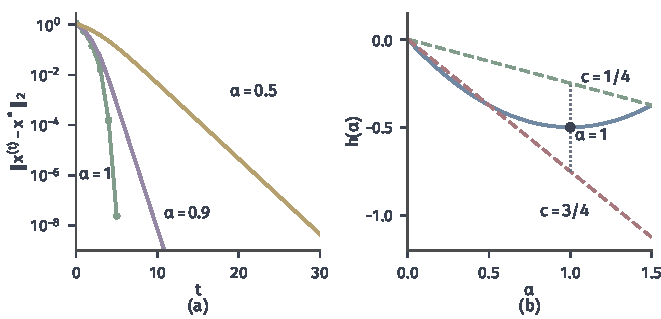
\includegraphics[width=112mm]{figures/05-optimization/02-smooth-optimization/matplotlib/newton-unit-step/figure.pdf}
  \caption{完整步的作用。(a)目标~\eqref{eq:newton-running-objective}上从$(\tfrac12,0)$出发、使用固定步长的距离误差：绿线$\alpha=1$，紫线$\alpha=0.9$，黄线$\alpha=0.5$。(b)二次目标沿Newton方向的变化量$h(\alpha)$（蓝，取$\omega^2=1$），绿色和红色虚线分别是$c=\tfrac14$和$c=\tfrac34$的Armijo线。$\alpha=1$处的黑点在绿线下方、红线上方，所以前者接受、后者拒绝。}
  \label{fig:newton-unit-step}
\end{BookInlineFigure}

回溯只需要函数值，每次试探一次函数计算。Newton方向的尺度已经带上了曲率信息，试探通常一两次就结束，所以这里用Armijo条件就够了。第~\ref{chap:smooth-foundations}章中要求方向导数的线搜索条件，主要用在方向尺度不明确或曲率更新需要额外保证的方法上。

\section{修正Newton法}
\label{sec:newton-modified}

上一节假定Hessian正定。这就需要回答：Hessian不定或接近奇异时，方向本身已经不可用，怎样改造曲率矩阵，既得到可靠的下降方向，又不破坏解附近的快速收敛？

\paragraph{缩短步长为什么不够}
在目标~\eqref{eq:newton-running-objective}的点$\bm{x}=(-\tfrac12,\tfrac34)$处，$u=\tfrac12$，由式~\eqref{eq:newton-running-derivatives}，
\[
 \bm{g}=\begin{bmatrix}-\tfrac12\\1\end{bmatrix},\qquad
 \bm{H}=\begin{bmatrix}1&2\\2&2\end{bmatrix}.
\]
$\bm{H}$的行列式是$-2$，特征值约为$3.56$和$-0.56$，不定。由式~\eqref{eq:newton-running-direction}，Newton方向是$\bm{d}=(-1.5,1)$，方向导数为
\[
 \bm{g}^\top\bm{d}=0.75+1=1.75>0.
\]
这是上坡方向，无论步长取多小，目标都上升。图~\ref{fig:newton-directions}中红色箭头正是这个方向，它指向离解更远的地方。

Hessian接近奇异时情形相反：方向是下坡的，但$\lVert\bm{d}\rVert_2$大得离谱。上一节$(-1,\tfrac65)$处的方向长度超过$22$，回溯要试探五次才找到可接受的步长。

问题出在模型的形状。负曲率方向上碗是倒扣的，几乎平坦的方向上碗底远在天边。于是不改步长，改曲率矩阵。

\paragraph{用正定矩阵代替Hessian}
\term{修正Newton法}（modified Newton method）用一个正定矩阵$\bm{B}^{(t)}$代替$\bm{H}^{(t)}$，解
\begin{equation}
 \bm{B}^{(t)}\bm{d}^{(t)}=-\bm{g}^{(t)},\qquad \bm{B}^{(t)}=\bm{H}^{(t)}+\bm{E}^{(t)}\succ\bm{0}.
 \label{eq:newton-modified-equation}
\end{equation}
其中$\bm{E}^{(t)}$是修正量。方向导数是
\[
 (\bm{g}^{(t)})^\top\bm{d}^{(t)}=-(\bm{g}^{(t)})^\top(\bm{B}^{(t)})^{-1}\bm{g}^{(t)}.
\]
$\bm{B}^{(t)}$正定，所以只要$\bm{g}^{(t)}\neq\bm{0}$，方向就是下降方向，上一节的回溯可以照用。

修正量的选择要在两种需求之间平衡。一方面希望$\bm{E}^{(t)}$足够大，让$\bm{B}^{(t)}$的条件数不太差。另一方面希望$\bm{E}^{(t)}$尽量小，因为它越大，模型离真实的曲率越远。Hessian本来就足够正定时，应当令$\bm{E}^{(t)}=\bm{0}$。下面三种常见做法，差别在于用什么代价换来多少修正。

\paragraph{对角平移}
最简单的修正是取$\bm{E}^{(t)}=\delta^{(t)}\bm{I}$：
\begin{equation}
 \bm{B}^{(t)}=\bm{H}^{(t)}+\delta^{(t)}\bm{I},\qquad \delta^{(t)}>\max\bigl\{0,-\lambda_{\min}(\bm{H}^{(t)})\bigr\}.
 \label{eq:newton-shift}
\end{equation}
所有特征值都加上$\delta^{(t)}$，特征向量不变。把$\bm{g}^{(t)}$按$\bm{H}^{(t)}$的正交特征向量$\bm{q}_i$展开，方向可以写成
\[
 \bm{d}(\delta)=-\sum_{i=1}^n\frac{\bm{q}_i^\top\bm{g}^{(t)}}{\lambda_i+\delta}\bm{q}_i.
\]

从这个式子可以读出$\delta$的作用。$\delta$很小时接近Newton方向。$\delta$远大于所有$\lvert\lambda_i\rvert$时，$\bm{d}(\delta)\approx-\bm{g}^{(t)}/\delta$，退化成短的负梯度步。所以$\delta$是在Newton方向和梯度方向之间连续调节的旋钮，调大它，步子变短，方向转向负梯度。

取Hessian正定但接近奇异的点$(-1,\tfrac65)$，特征值约为$0.039$和$10.16$。表~\ref{tab:newton-shift-values}列出几个$\delta$下的结果，图~\ref{fig:newton-shift-effects}(a)画出长度的变化。$\delta$越过小特征值$0.039$后，长度迅速下降。$\delta=1$的完整步就把目标从$2.04$降到$1.231$，比不修正时好得多；$\delta=100$时几乎不动。

\begin{BookInlineTable}
  \centering
  \begin{tabular}{@{}cccc@{}}
    \toprule
    $\delta$ & $\bm{d}(\delta)$ & $\lVert\bm{d}(\delta)\rVert_2$ & $f(\bm{x}+\bm{d}(\delta))$ \\
    \midrule
    $0$ & $(10,-20.2)$ & $22.54$ & $10032$ \\
    $0.1$ & $(2.881,-5.678)$ & $6.367$ & $64.66$ \\
    $1$ & $(0.448,-0.731)$ & $0.858$ & $1.231$ \\
    $10$ & $(0.0791,-0.0597)$ & $0.0991$ & $1.930$ \\
    $100$ & $(0.0113,-0.0044)$ & $0.0121$ & $2.025$ \\
    \bottomrule
  \end{tabular}
  \caption{在$\bm{x}=(-1,\tfrac65)$处对角平移的效果，出发点的目标值是$2.04$。修正太小方向过长，修正太大几乎原地不动。}
  \label{tab:newton-shift-values}
\end{BookInlineTable}

\begin{BookInlineFigure}
  \centering
  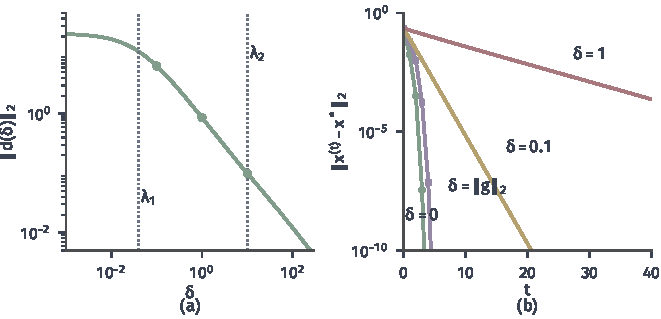
\includegraphics[width=112mm]{figures/05-optimization/02-smooth-optimization/matplotlib/newton-shift-effects/figure.pdf}
  \caption{对角平移的两个效应。(a)在$(-1,\tfrac65)$处方向长度随$\delta$的变化，灰色竖线是Hessian的两个特征值，绿点对应$\delta=0.1,1,10$。(b)从$(0.9,0.8)$出发、使用完整步的距离误差：绿线$\delta=0$，紫线$\delta=\lVert\bm{g}\rVert_2$，黄线$\delta=0.1$，红线$\delta=1$。修正量不消失时收敛只有线性。}
  \label{fig:newton-shift-effects}
\end{BookInlineFigure}

实际上不必先算$\lambda_{\min}$。尝试对$\bm{H}^{(t)}+\delta\bm{I}$作Cholesky分解：分解成功说明已经正定，遇到非正主元就增大$\delta$再试。这正是后面计算过程采用的做法。

\paragraph{谱修正}
对角平移把所有特征值一起抬高，也改动了本来很好的方向。如果能算出谱分解$\bm{H}^{(t)}=\bm{Q}\bm{\Lambda}\bm{Q}^\top$，就可以只改有问题的特征值，这称为\term{谱修正}（spectral modification）：
\begin{equation}
 \bm{B}^{(t)}=\bm{Q}\tilde{\bm{\Lambda}}\bm{Q}^\top,\qquad
 \tilde\lambda_i=\max\bigl\{\lvert\lambda_i\rvert,\ \epsilon\bigr\}.
 \label{eq:newton-spectral}
\end{equation}
其中$\epsilon>0$是下限。取绝对值的含义是：负曲率方向上，模型的碗是倒扣的，那就翻过来，弯度的大小不变。Newton方向在这个特征方向上的分量$-\bm{q}_i^\top\bm{g}/\lambda_i$指向鞍点，翻转后变为$-\bm{q}_i^\top\bm{g}/\lvert\lambda_i\rvert$，朝下坡方向走。

图~\ref{fig:newton-spectral-maps}比较三种常见的特征值映射。只把小于下限的值截到$\epsilon$也是一种选择，但在负曲率方向上会得到很大的步。在$(-\tfrac12,\tfrac34)$处，取$\epsilon=0.1$的截断规则给出的方向是$(7.87,-6.32)$，比取绝对值得到的$(1.33,-1.21)$长了好几倍。

\begin{BookInlineFigure}
  \centering
  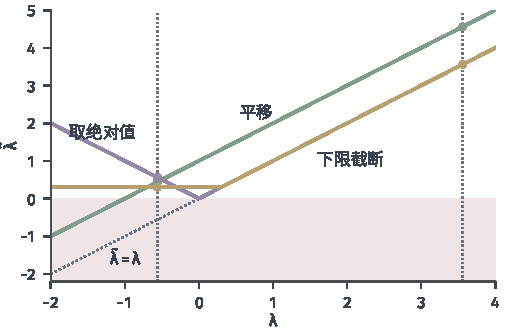
\includegraphics[width=86mm]{figures/05-optimization/02-smooth-optimization/matplotlib/newton-spectral-maps/figure.pdf}
  \caption{特征值$\lambda$经修正后的值$\tilde\lambda$。绿线是平移$\delta=1$，紫线是取绝对值，黄线是下限截断$\max\{\lambda,0.3\}$，灰色点线是不修正。竖线标出$(-\tfrac12,\tfrac34)$处Hessian的两个特征值，三条线上的点是修正后的值。红色浅底是不允许的非正区域。}
  \label{fig:newton-spectral-maps}
\end{BookInlineFigure}

谱修正的修正量最贴合问题，但要计算完整的特征分解，稠密时的常数比Cholesky分解大得多。

\paragraph{修正Cholesky分解}
第三种做法把修正放进分解过程。在作$\bm{L}\bm{D}\bm{L}^\top$分解时，第$j$步的主元$c_j$如果太小或为负，就把它换成正数，分解继续往下走。这称为\term{修正Cholesky分解}（modified Cholesky factorization），得到的$\bm{B}=\bm{L}\bm{D}\bm{L}^\top$自动正定，分解已经完成，成本与普通分解同量级。

在$(-\tfrac12,\tfrac34)$处。第一个主元是$c_1=1$，消元乘子是$\ell_{21}=2$，第二个主元是
\[
 c_2=2-\ell_{21}^2c_1=2-4=-2.
\]
这个主元为负，普通Cholesky分解在此失败。把它换成绝对值$d_2=2$，得到
\[
 \bm{B}=\begin{bmatrix}1&0\\2&1\end{bmatrix}
 \begin{bmatrix}1&0\\0&2\end{bmatrix}
 \begin{bmatrix}1&2\\0&1\end{bmatrix}
 =\begin{bmatrix}1&2\\2&6\end{bmatrix}.
\]
相当于只修改了右下角元素，$\bm{E}=\operatorname{diag}(0,4)$。

简单地“遇到负主元就取绝对值”可能带来很大的修正，因为小主元会放大后面的元素。取
\[
 \bm{H}=\begin{bmatrix}0.01&1\\1&0\end{bmatrix},
\]
它的特征值约为$\pm1$，平移量$1$多一点就够。可是$c_1=0.01$是正的，不作修改，于是$\ell_{21}=100$，$c_2=0-100^2\times0.01=-100$。取绝对值之后$\bm{B}$的右下角是$\ell_{21}^2c_1+d_2=200$，修正量高达$200$。

办法是同时限制消元乘子的大小。记$\theta_j=\max_{i>j}\lvert c_{ij}\rvert$为第$j$列主元下方尚未除以主元的元素的最大绝对值，给定上界$\bar\beta>0$和下限$\hat\delta>0$，取
\begin{equation}
 d_j=\max\Bigl\{\lvert c_j\rvert,\ \frac{\theta_j^2}{\bar\beta^2},\ \hat\delta\Bigr\}.
 \label{eq:newton-modified-cholesky-pivot}
\end{equation}
上面的例子取$\bar\beta=1$。第一列$\theta_1=1$，所以$d_1=\max\{0.01,1,\hat\delta\}=1$，$\ell_{21}=1$。第二个主元是$c_2=0-1=-1$，$d_2=1$。最后得到
\[
 \bm{B}=\begin{bmatrix}1&1\\1&2\end{bmatrix},\qquad \bm{E}=\operatorname{diag}(0.99,\,2).
\]
修正量降到与$\lvert\lambda_{\min}\rvert$同一量级。参数怎样选择才能在理论上控制$\lVert\bm{E}\rVert$，证明较长，读者可查阅\scite{math-nocedal2006numerical}。

\paragraph{三种修正的比较}
图~\ref{fig:newton-directions}和表~\ref{tab:newton-correction-compare}在同一点比较三种修正。三个方向都转向了下坡，都需要回溯一次，$\alpha=1$都被拒绝，$\alpha=\tfrac12$都被接受。这一点上修正Cholesky分解的新点目标值最低，这只是这一步的结果，不代表它总是更好。

\begin{BookInlineFigure}
  \centering
  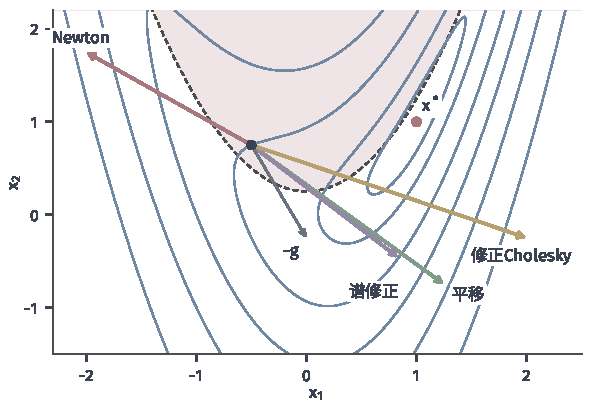
\includegraphics[width=100mm]{figures/05-optimization/02-smooth-optimization/matplotlib/newton-directions/figure.pdf}
  \caption{$\bm{x}=(-\tfrac12,\tfrac34)$（黑点）处的几种方向，箭头按实际长度绘制。红色是未修正的Newton方向，指向上坡。绿色、紫色、黄色分别是对角平移$\delta=1$、谱修正（取绝对值）、修正Cholesky分解得到的方向，灰色是负梯度。蓝线是等高线，红色浅底是Hessian不定的区域，红点是解。}
  \label{fig:newton-directions}
\end{BookInlineFigure}

\begin{BookInlineTable}
  \centering
  \begin{tabular}{@{}lccccc@{}}
    \toprule
    做法 & $\lVert\bm{E}\rVert_2$ & $\bm{d}$ & $\bm{g}^\top\bm{d}$ & $\alpha$ & 新点$f$ \\
    \midrule
    对角平移$\delta=1$ & $1$ & $(1.75,-1.5)$ & $-2.375$ & $\tfrac12$ & $0.2151$ \\
    谱修正（绝对值） & $1.123$ & $(1.334,-1.213)$ & $-1.880$ & $\tfrac12$ & $0.3604$ \\
    修正Cholesky & $4$ & $(2.5,-1)$ & $-2.25$ & $\tfrac12$ & $0.1289$ \\
    \bottomrule
  \end{tabular}
  \caption{在$(-\tfrac12,\tfrac34)$处三种修正的结果，出发点目标值$1.375$，回溯参数$c=0.1$，$\beta=0.5$。}
  \label{tab:newton-correction-compare}
\end{BookInlineTable}

\paragraph{计算过程}
下面以对角平移为例写出完整算法，它只用Cholesky分解试探，不需要特征值。$\delta$的试探规则如下：对角元都为正时从$0$开始试；否则从$-\min_ih_{ii}+b$开始，$b>0$是一个固定的基准量；分解失败时令$\delta\leftarrow\max\{2\delta,b\}$。

\needspace{6\baselineskip}
\paragraph{变量}
\begin{itemize}
 \item $\bm{x},\bm{g},\bm{H}$：当前点、梯度、Hessian。
 \item $\delta$：本轮的对角平移量，每轮重新确定。
 \item $\bm{L}$：$\bm{H}+\delta\bm{I}$的Cholesky因子。
 \item $\bm{d}$：修正后的方向。
 \item $\alpha,c,\beta$：回溯所用的量，与上一节相同。
 \item $b$：平移基准量，例中取$1$。
\end{itemize}

\paragraph{初始化}
选定$\bm{x}^{(0)}$和各参数。例中取下面的数据：
\[
 \bm{x}^{(0)}=\bigl(-\tfrac12,\tfrac34\bigr),\qquad b=1,\qquad c=0.1,\qquad \beta=0.5,\qquad \varepsilon=10^{-6}.
\]

\needspace{6\baselineskip}
\paragraph{每轮更新}
在第$t$轮：
\begin{enumerate}
 \item \textbf{读取导数并检查停止。}计算$\bm{g}^{(t)}$、$\bm{H}^{(t)}$，若$\lVert\bm{g}^{(t)}\rVert_2\leq\varepsilon$，输出$\bm{x}^{(t)}$并结束。

 例中第一轮的数据已在本节开头列出。

 \item \textbf{确定平移量。}按上述规则试探，直到Cholesky分解成功，得到$\delta^{(t)}$和$\bm{L}$。

 例中第一轮对角元都为正，先试$\delta=0$，第二个主元$2-4=-2$，分解失败。再试$\delta=1$，矩阵和因子为
 \[
  \bm{H}+\bm{I}=\begin{bmatrix}2&2\\2&3\end{bmatrix},\qquad
  \bm{L}=\begin{bmatrix}\sqrt2&0\\\sqrt2&1\end{bmatrix},
 \]
 分解成功，$\delta^{(0)}=1$。

 \item \textbf{求方向。}前代、回代解方程~\eqref{eq:newton-modified-equation}。

 例中第一轮解$2d_1+2d_2=\tfrac12$，$2d_1+3d_2=-1$，得到
 \[
  \bm{d}^{(0)}=\begin{bmatrix}1.75\\-1.5\end{bmatrix}.
 \]

 \item \textbf{回溯并更新。}从$\alpha=1$开始按式~\eqref{eq:newton-armijo}回溯，然后更新$\bm{x}$，令$t\leftarrow t+1$。

 例中第一轮方向导数为$-2.375$。试$\alpha=1$，新点目标值$5.379$，高于右端$1.1375$，拒绝。试$\alpha=\tfrac12$，新点是$(\tfrac38,0)$，目标值$0.2151$，低于右端$1.2563$，接受。

 第二轮$u=-\tfrac9{64}$，$1-4u=\tfrac{25}{16}>0$，Hessian已经正定，$\delta^{(1)}=0$的分解成功。方向就是Newton方向，由式~\eqref{eq:newton-running-direction}，
 \[
  d_1=\frac{5/8}{25/16}=\frac25,\qquad d_2=\frac9{64}+\frac34\cdot\frac25=0.440625.
 \]
 完整步被接受，到达$(0.775,0.440625)$，目标值$0.0509$。
\end{enumerate}

各轮结果见表~\ref{tab:newton-modified-run}。修正只在第一轮出现，第$6$轮梯度范数低于容差，迭代结束，最终得到$\bm{x}^{(6)}\approx(1,1)$。图~\ref{fig:newton-modified-path}是这条路径。

\begin{BookInlineTable}
  \centering
  \begin{tabular}{@{}ccccc@{}}
    \toprule
    $t$ & $\bm{x}^{(t)}$ & $f$ & $\delta^{(t)}$ & $\alpha^{(t)}$ \\
    \midrule
    $0$ & $(-0.5,0.75)$ & $1.375$ & $1$ & $1/2$ \\
    $1$ & $(0.375,0)$ & $0.2151$ & $0$ & $1$ \\
    $2$ & $(0.775,0.4406)$ & $0.05091$ & $0$ & $1$ \\
    $3$ & $(0.9122,0.8133)$ & $4.21\mathrm{e}{-3}$ & $0$ & $1$ \\
    $4$ & $(0.9939,0.9811)$ & $6.34\mathrm{e}{-5}$ & $0$ & $1$ \\
    $5$ & $(0.99984,0.99965)$ & $1.40\mathrm{e}{-8}$ & $0$ & $1$ \\
    $6$ & $(1.0000,1.0000)$ & $9.1\mathrm{e}{-16}$ & 停止 & \\
    \bottomrule
  \end{tabular}
  \caption{对角平移的修正Newton法从$(-\tfrac12,\tfrac34)$出发的迭代，只有第一轮需要修正和回溯。}
  \label{tab:newton-modified-run}
\end{BookInlineTable}

\begin{BookInlineFigure}
  \centering
  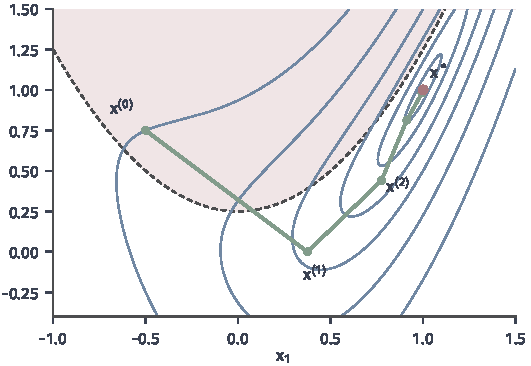
\includegraphics[width=90mm]{figures/05-optimization/02-smooth-optimization/matplotlib/newton-modified-path/figure.pdf}
  \caption{修正Newton法的路径（绿）。起点$(-\tfrac12,\tfrac34)$在Hessian不定的红色浅底区域内，第一步用$\delta=1$的修正方向并取步长$\tfrac12$，落入正定区域后修正消失，以后都是完整的Newton步。蓝线是等高线，红点是解。}
  \label{fig:newton-modified-path}
\end{BookInlineFigure}

\paragraph{全局性质：一致有界的修正}
修正之后方向不再是Newton方向，上一节的定理不能直接用。下面的结论只要求修正后的矩阵特征值一致有界，不要求目标凸，这正是修正要达到的目的。

\begin{theorem}[修正方向的全局收敛]
\label{thm:newton-modified-global}
设$f$有下界，$\nabla f$是$L$-Lipschitz的，存在$0<b\leq\bar b$，使各轮$b\bm{I}\preceq\bm{B}^{(t)}\preceq\bar b\bm{I}$。方向由方程~\eqref{eq:newton-modified-equation}给出，步长由Armijo回溯确定，$c\in(0,1)$，$\beta\in(0,1)$，初始试探为$1$。记
\begin{equation}
 \alpha_{\min}=\min\Bigl\{1,\ \frac{2\beta(1-c)b^2}{L\bar b}\Bigr\}.
 \label{eq:newton-alpha-min}
\end{equation}
则
\begin{equation}
 \min_{0\leq t\leq T}\lVert\bm{g}^{(t)}\rVert_2^2\leq\frac{\bar b\,\bigl(f(\bm{x}^{(0)})-\inf f\bigr)}{c\,\alpha_{\min}\,(T+1)}.
 \label{eq:newton-modified-rate}
\end{equation}
特别地，$\lVert\bm{g}^{(t)}\rVert_2\to0$。
\end{theorem}

\begin{proof}
省略上标。梯度$L$-Lipschitz给出二次上界
\[
 f(\bm{x}+\alpha\bm{d})\leq f(\bm{x})+\alpha\bm{g}^\top\bm{d}+\frac L2\alpha^2\lVert\bm{d}\rVert_2^2.
\]
与Armijo条件比较，只要
\[
 \alpha\leq\frac{2(1-c)\lvert\bm{g}^\top\bm{d}\rvert}{L\lVert\bm{d}\rVert_2^2},
\]
条件就成立。

由特征值的界，方向导数和方向长度满足
\[
 \lvert\bm{g}^\top\bm{d}\rvert=\bm{g}^\top\bm{B}^{-1}\bm{g}\geq\frac{\lVert\bm{g}\rVert_2^2}{\bar b},\qquad
 \lVert\bm{d}\rVert_2\leq\frac{\lVert\bm{g}\rVert_2}{b}.
\]
于是上述门槛不小于$2(1-c)b^2/(L\bar b)$。回溯的步长要么是初始的$1$，要么是一个被拒绝的值乘以$\beta$，所以$\alpha\geq\alpha_{\min}$。

代入Armijo条件，每轮下降量满足
\[
 f(\bm{x})-f(\bm{x}^{(t+1)})\geq c\,\alpha_{\min}\frac{\lVert\bm{g}\rVert_2^2}{\bar b}.
\]
对$t=0,\ldots,T$求和，左端不超过$f(\bm{x}^{(0)})-\inf f$，最小值不超过平均值，即得式~\eqref{eq:newton-modified-rate}。由于级数$\sum_t\lVert\bm{g}^{(t)}\rVert_2^2$收敛，通项趋于零。
\end{proof}

结论只说梯度趋于零，极限点可能是鞍点。在鞍点处$\bm{g}^{(t)}=\bm{0}$，方程~\eqref{eq:newton-modified-equation}的解是零向量，无论怎样修正都不会动。怎样从鞍点离开，是第~\ref{chap:saddle-points}章的问题。

\paragraph{修正何时消失}
修正对局部速度的影响可以精确写出来。设$\bm{e}=\bm{x}^{(t)}-\bm{x}^\star$，$\bm{B}=\bm{H}^{(t)}+\bm{E}$，步长为$1$。照定理~\ref{thm:newton-local}证明的做法，得到
\[
 \bm{x}^{(t+1)}-\bm{x}^\star=\bm{B}^{-1}\Bigl[\int_0^1\bigl(\bm{H}^{(t)}-\nabla^2f(\bm{x}^\star+s\bm{e})\bigr)\bm{e}\,\mathrm{d}s+\bm{E}\bm{e}\Bigr].
\]
方括号中第一项是模型的二次误差，第二项是修正带来的一次误差。若$\lVert\bm{B}^{-1}\rVert_2$一致有界，就得到
\begin{equation}
 \lVert\bm{x}^{(t+1)}-\bm{x}^\star\rVert_2\leq\lVert\bm{B}^{-1}\rVert_2\Bigl(\frac M2\lVert\bm{e}\rVert_2^2+\lVert\bm{E}\rVert_2\lVert\bm{e}\rVert_2\Bigr).
 \label{eq:newton-modified-local}
\end{equation}

由此可以逐条读出修正的三种结局。若$\bm{E}$有限步后为零，则恢复二次收敛。若修正量趋于零，收敛是超线性的。若修正量与误差同阶，仍然是二次收敛。修正量不消失时只有线性收敛：在特征值为$\lambda$的方向上，$\bm{E}=\delta\bm{I}$的误差因子是$\delta/(\lambda+\delta)$。

主例解处的小特征值约为$0.185$。取$\delta=0.1$时因子约$0.35$，取$\delta=1$时约$0.84$，图~\ref{fig:newton-shift-effects}(b)中黄线和红线的斜率正是如此。紫线取$\delta=\lVert\bm{g}\rVert_2$，修正量随误差同阶消失，仍然以二次速度收敛。

所以修正Newton法必须满足一个要求：Hessian足够正定时要退回不修正。上面的试探规则总是先试$\delta=0$，正好满足这一点。若$\nabla^2f(\bm{x}^\star)\succ\bm{0}$，在解附近分解一次成功，迭代就成为纯粹的Newton法。使用谱修正时，下限$\epsilon$要小于$\lambda_{\min}(\nabla^2f(\bm{x}^\star))$，否则修正不会消失。

\paragraph{改迭代与改目标}
把$\bm{H}^{(t)}$换成$\bm{H}^{(t)}+\delta\bm{I}$，方程很像给目标加了正则项$\tfrac\delta2\lVert\bm{x}\rVert_2^2$之后的Newton方程，两件事却完全不同。下面用一元目标$f(x)=\tfrac12(x-1)^2$比较。

修正迭代时，$x^{(t+1)}=x^{(t)}-(x^{(t)}-1)/(1+\delta)$，极限仍是$1$，只是收敛变慢。改目标时，新目标的最小点是$1/(1+\delta)$，解已经变了。

\begin{BookInlineTable}
  \centering
  \begin{tabular}{@{}lll@{}}
    \toprule
    & 修正迭代 & 改变目标 \\
    \midrule
    方程右端 & 原梯度$-\bm{g}^{(t)}$ & 新目标的梯度$-\bm{g}^{(t)}-\delta\bm{x}^{(t)}$ \\
    驻点 & 与原目标相同 & 通常移动 \\
    作用 & 让方向可用 & 改变要解的问题 \\
    \bottomrule
  \end{tabular}
  \caption{曲率修正和正则化的区别。修正只影响路径，不影响梯度为零的点。}
  \label{tab:newton-modify-vs-regularize}
\end{BookInlineTable}

平移量$\delta$还可以根据模型预测准不准来自动调整，这与直接限制位移的长度密切相关，将在第~\ref{chap:trust-region}章讨论。

\section{非精确Newton法}
\label{sec:newton-inexact}

前面三节都假定方程能精确解出。当$n$很大、完整的Hessian存不下或分解不起时，线性方程只解到什么程度就够了，这样做对收敛速度有什么影响？

一个直观的想法是：Newton方程本身只是对原问题的局部近似，离解远的时候，把这个近似方程解到机器精度并没有意义。比如$n=10^5$的稠密Hessian要存$10^{10}$个数，分解一次要约$3\times10^{14}$次运算。如果迭代法几十次矩阵向量乘积就能给出足够好的方向，就没有必要付出这个代价。

\subsection{内层精度的控制}
\label{sec:newton-forcing}

\paragraph{用残差规定精度}
设内层算法给出的方向是$\bm{d}^{(t)}$。它对Newton方程的满足程度用残差来衡量：
\begin{equation}
 \bm{r}^{(t)}=\bm{H}^{(t)}\bm{d}^{(t)}+\bm{g}^{(t)}.
 \label{eq:newton-residual}
\end{equation}
\term{非精确Newton法}（inexact Newton method）不要求$\bm{r}^{(t)}=\bm{0}$，只要求残差相对于梯度足够小：
\begin{equation}
 \lVert\bm{H}^{(t)}\bm{d}^{(t)}+\bm{g}^{(t)}\rVert_2\leq\eta_t\lVert\bm{g}^{(t)}\rVert_2,
 \label{eq:newton-inexact-condition}
\end{equation}
其中$\eta_t\in[0,1)$称为\term{误差比例}（forcing term）。零向量的残差就是$\bm{g}^{(t)}$，对应比例$1$，所以$\eta_t<1$表示“至少比什么都不做强一点”。$\eta_t=0$就是精确的Newton法。

用比例而不用绝对容差，是因为要求应当随迭代变化。梯度大时方程的右端大，粗略的解就够了；梯度小时，同样的相对精度自动要求更小的绝对误差。

\paragraph{比例要多小：一个局部定理}
和定理~\ref{thm:newton-local}一样，这里需要解附近的非退化和Hessian的Lipschitz条件。这次用$\bm{A}=\nabla^2f(\bm{x}^\star)$加权的误差$\lVert\bm{A}\bm{e}\rVert_2$来度量。在解附近，$\bm{g}\approx\bm{A}\bm{e}$，所以这个量就是一阶近似下的梯度范数，与条件~\eqref{eq:newton-inexact-condition}用的是同一把尺子。

\begin{theorem}[非精确Newton法的局部收敛]
\label{thm:newton-inexact-local}
设$f$在开球$\lVert\bm{x}-\bm{x}^\star\rVert_2<r$上二阶连续可微，$\nabla f(\bm{x}^\star)=\bm{0}$，$\bm{A}=\nabla^2f(\bm{x}^\star)\succeq\mu\bm{I}$，$\mu>0$，Hessian是$M$-Lipschitz的。记$\bm{e}^{(t)}=\bm{x}^{(t)}-\bm{x}^\star$，以及
\begin{equation}
 s_t=\lVert\bm{A}\bm{e}^{(t)}\rVert_2,\qquad \rho_t=\frac{Ms_t}{\mu^2}.
 \label{eq:newton-inexact-quantities}
\end{equation}
若$s_t<\min\{\mu r,\ \mu^2/(2M)\}$，$\eta_t\in[0,1]$，$\bm{d}^{(t)}$满足条件~\eqref{eq:newton-inexact-condition}，$\bm{x}^{(t+1)}=\bm{x}^{(t)}+\bm{d}^{(t)}$，则
\begin{equation}
 s_{t+1}\leq(1+2\rho_t)(\eta_t+\rho_t)\,s_t.
 \label{eq:newton-inexact-bound}
\end{equation}
\end{theorem}

\begin{proof}
省略上标，记$\bm{e}=\bm{e}^{(t)}$，$s=s_t$，$\rho=\rho_t$，$\bm{H}=\bm{H}^{(t)}$。

第一步是准备。由$\bm{A}\succeq\mu\bm{I}$得$\lVert\bm{e}\rVert_2\leq s/\mu$，因此点在球内，并且$\lVert\bm{e}\rVert_2<\mu/(2M)$。由Hessian的Lipschitz条件，
\[
 \lVert\bm{H}-\bm{A}\rVert_2\leq M\lVert\bm{e}\rVert_2\leq\frac\mu2,\qquad \lVert\bm{H}^{-1}\rVert_2\leq\frac2\mu.
\]

第二步把梯度写成线性部分加小量。沿线段积分，$\bm{g}=\bm{A}\bm{e}+\bm{q}_1$，其中
\[
 \bm{q}_1=\int_0^1\bigl(\nabla^2f(\bm{x}^\star+\sigma\bm{e})-\bm{A}\bigr)\bm{e}\,\mathrm{d}\sigma,\qquad
 \lVert\bm{q}_1\rVert_2\leq\frac M2\lVert\bm{e}\rVert_2^2\leq\frac{\rho s}2.
\]
最后一步用了$\lVert\bm{e}\rVert_2\leq s/\mu$和$\rho$的定义。于是残差的界是
\[
 \lVert\bm{r}\rVert_2\leq\eta\lVert\bm{g}\rVert_2\leq\eta\Bigl(1+\frac\rho2\Bigr)s.
\]

第三步写出新误差。由$\bm{d}=\bm{H}^{-1}(\bm{r}-\bm{g})$，
\[
 \bm{e}+\bm{d}=\bm{H}^{-1}(\bm{r}+\bm{q}_2),\qquad \bm{q}_2=\bm{H}\bm{e}-\bm{g}.
\]
与定理~\ref{thm:newton-local}证明中的积分相同，
\[
 \lVert\bm{q}_2\rVert_2\leq\frac M2\lVert\bm{e}\rVert_2^2\leq\frac{\rho s}2.
\]

第四步转到加权误差。在$\bm{e}+\bm{d}$上左乘$\bm{A}$，并把$\bm{A}$写成$\bm{H}+(\bm{A}-\bm{H})$，得到
\[
 \bm{A}(\bm{e}+\bm{d})=\bigl(\bm{I}+(\bm{A}-\bm{H})\bm{H}^{-1}\bigr)(\bm{r}+\bm{q}_2).
\]
括号中第一个因子的范数不超过$1+M\lVert\bm{e}\rVert_2\cdot2/\mu\leq1+2\rho$。第二个因子的范数不超过
\[
 \eta\Bigl(1+\frac\rho2\Bigr)s+\frac{\rho s}2\leq(\eta+\rho)s,
\]
这里用了$\eta\leq1$。两者相乘即得式~\eqref{eq:newton-inexact-bound}。
\end{proof}

式~\eqref{eq:newton-inexact-bound}把收缩比拆成两部分：$\eta_t$来自线性方程的残差，$\rho_t$来自Taylor误差。由此读出三种情形。

第一种，$\eta_t\leq\bar\eta<1$。取$\bar\rho\in(0,\tfrac12]$足够小，使$(1+2\bar\rho)(\bar\eta+\bar\rho)=\bar\theta<1$。只要起始的$s_0$足够小，使$\rho_0\leq\bar\rho$，$s_t$就逐步减小，并且
\[
 s_{t+1}\leq\bar\theta\,s_t.
\]
这是线性收敛，收缩比接近$\bar\eta$。

第二种，$\eta_t\to0$。此时$s_t\to0$，$\rho_t\to0$，于是
\[
 \frac{s_{t+1}}{s_t}\leq(1+2\rho_t)(\eta_t+\rho_t)\to0.
\]
比值趋于零的收敛称为\term{超线性收敛}（superlinear convergence）。

第三种，$\eta_t\leq C\lVert\bm{g}^{(t)}\rVert_2$。由第二步和$\rho_t\leq\tfrac12$，
\[
 \lVert\bm{g}^{(t)}\rVert_2\leq\Bigl(1+\frac{\rho_t}2\Bigr)s_t\leq\frac54s_t.
\]
代入式~\eqref{eq:newton-inexact-bound}，利用$1+2\rho_t\leq2$，得到
\[
 s_{t+1}\leq2\Bigl(\frac54C+\frac M{\mu^2}\Bigr)s_t^2.
\]
这是二次收敛。一般地，$\eta_t\leq C\lVert\bm{g}^{(t)}\rVert_2^{\theta}$（$0<\theta\leq1$）给出$1+\theta$阶收敛。

实际中常用的比例是
\begin{equation}
 \eta_t=\min\bigl\{0.5,\sqrt{\lVert\bm{g}^{(t)}\rVert_2}\bigr\}
 \quad\text{或}\quad
 \eta_t=\min\bigl\{0.5,\lVert\bm{g}^{(t)}\rVert_2\bigr\}.
 \label{eq:newton-forcing-rule}
\end{equation}
前者是超线性收敛，后者是二次收敛\scite{math-nocedal2006numerical}。这样远离解时内层只做很少的工作，接近解时才逐步加严，避免把精力浪费在一个并不准确的模型上。

图~\ref{fig:newton-eta-rates}在目标~\eqref{eq:newton-running-objective}上验证这些结论。为了让残差比例恰好等于$\eta_t$，这里取$\bm{r}^{(t)}=\eta_t\bm{g}^{(t)}$，此时方向等于$(1-\eta_t)$倍的Newton方向。比例取常数时，收缩比稳定在该常数附近；比例趋于零时收缩比也趋于零。

\begin{BookInlineFigure}
  \centering
  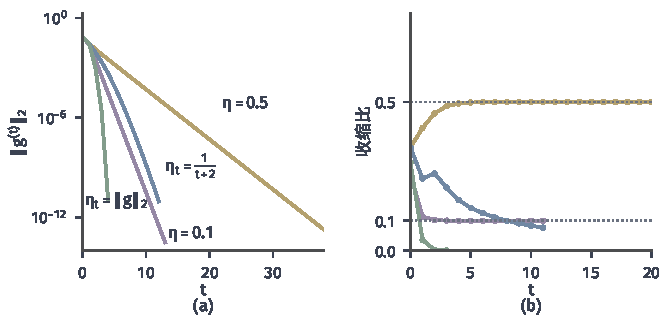
\includegraphics[width=112mm]{figures/05-optimization/02-smooth-optimization/matplotlib/newton-eta-rates/figure.pdf}
  \caption{误差比例对局部速度的影响，从$(0.9,0.8)$出发，残差取$\eta_t\bm{g}^{(t)}$。(a)梯度范数：黄线$\eta=0.5$、紫线$\eta=0.1$是直线，蓝线$\eta_t=1/(t+2)$越来越陡，绿线$\eta_t=\lVert\bm{g}^{(t)}\rVert_2$几步到底。(b)各线的收缩比$\lVert\bm{A}\bm{e}^{(t+1)}\rVert_2/\lVert\bm{A}\bm{e}^{(t)}\rVert_2$，灰色点线标出$0.5$和$0.1$。}
  \label{fig:newton-eta-rates}
\end{BookInlineFigure}

\paragraph{远离解时}
局部定理只说解附近。在远处，条件~\eqref{eq:newton-inexact-condition}本身甚至不保证方向下降。把$\bm{d}=\bm{H}^{-1}(\bm{r}-\bm{g})$代入方向导数，得到
\[
 \bm{g}^\top\bm{d}=-\bm{g}^\top\bm{H}^{-1}\bm{g}+\bm{g}^\top\bm{H}^{-1}\bm{r}.
\]
第二项的大小可以超过第一项。设$\bm{H}$正定，比较两项的界，能够保证方向导数为负的充分条件是$\eta_t<1/\kappa(\bm{H})$，这在病态时非常苛刻。

具体的例子如下。取
\[
 \bm{H}=\operatorname{diag}(1,100),\qquad \bm{g}=(1,10).
\]
Newton方向是$\bm{d}_{\mathrm{N}}=(-1,-0.1)$。取残差$\bm{r}=(2.5,0.25)$，比例为
\[
 \frac{\lVert\bm{r}\rVert_2}{\lVert\bm{g}\rVert_2}=\frac{2.5125}{10.050}=0.25.
\]
对应的方向是
\[
 \bm{d}=\bm{H}^{-1}(\bm{r}-\bm{g})=(1.5,-0.0975).
\]
它的方向导数是$\bm{g}^\top\bm{d}=1.5-0.975=0.525>0$，满足残差条件，却是上坡方向。

图~\ref{fig:newton-residual-ellipse}说明了原因。满足条件的方向构成以$\bm{d}_{\mathrm{N}}$为中心的椭球，半轴长度正比于$\eta\lVert\bm{g}\rVert_2/\lambda_i$。Hessian的小特征值方向上半轴很长，椭球可以越过$\bm{g}^\top\bm{d}=0$的分界面。

\begin{BookInlineFigure}
  \centering
  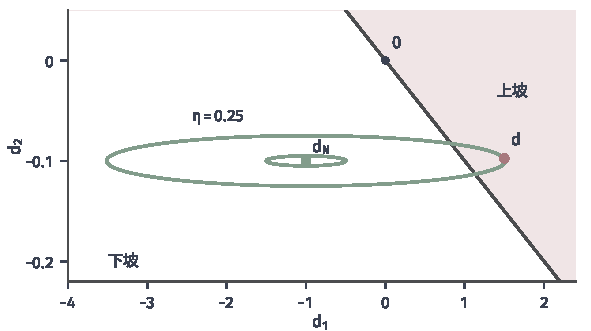
\includegraphics[width=100mm]{figures/05-optimization/02-smooth-optimization/matplotlib/newton-residual-ellipse/figure.pdf}
  \caption{方向空间中满足残差条件的集合，$\bm{H}=\operatorname{diag}(1,100)$，$\bm{g}=(1,10)$，注意两轴比例不同。绿色椭圆分别是$\eta=0.25$和$\eta=0.05$的边界，绿点是Newton方向，深灰色粗线是$\bm{g}^\top\bm{d}=0$，红色浅底是上坡方向的区域。红点$\bm{d}$的残差比例为$0.25$，却落在上坡区域内。}
  \label{fig:newton-residual-ellipse}
\end{BookInlineFigure}

因此远离解时还需要两样东西：内层算法要能保证给出下降方向，外层仍然要作线搜索。一般的迭代线性求解器并不提供前者，下一小节的共轭梯度法却恰好能提供。

\subsection{Newton-CG}
\label{sec:newton-cg}

\paragraph{主要思想}
Newton方程的系数矩阵对称，在解附近还正定，最自然的内层算法是共轭梯度法，这种组合称为\term{Newton-CG}（Newton conjugate gradient method）。它的吸引力在于，内层只需要能计算$\bm{H}^{(t)}$乘向量，完全不必形成矩阵。

共轭梯度法的完整推导可参考\BookChapterRef{chap:krylov-methods}{卷二第15章“Krylov子空间法”}，这里只复述用到的结论。为了和式~\eqref{eq:newton-residual}保持一致，把残差定义成$\bm{r}_j=\bm{H}\bm{z}_j+\bm{g}$。从$\bm{z}_0=\bm{0}$，$\bm{r}_0=\bm{g}$，$\bm{p}_0=-\bm{g}$出发，第$j$步计算
\begin{equation}
 \alpha_j=\frac{\bm{r}_j^\top\bm{r}_j}{\bm{p}_j^\top\bm{H}\bm{p}_j},\qquad
 \bm{z}_{j+1}=\bm{z}_j+\alpha_j\bm{p}_j,\qquad
 \bm{r}_{j+1}=\bm{r}_j+\alpha_j\bm{H}\bm{p}_j,
 \label{eq:newton-cg-step}
\end{equation}
\begin{equation}
 \beta_{j}=\frac{\bm{r}_{j+1}^\top\bm{r}_{j+1}}{\bm{r}_j^\top\bm{r}_j},\qquad
 \bm{p}_{j+1}=-\bm{r}_{j+1}+\beta_j\bm{p}_j.
 \label{eq:newton-cg-direction}
\end{equation}
这里$\alpha_j$沿$\bm{p}_j$精确极小化模型，每步新的残差与之前的方向正交，新的方向与之前的方向关于$\bm{H}$共轭。

\paragraph{Hessian向量积}
式~\eqref{eq:newton-cg-step}中对$\bm{H}$的唯一需求是计算乘积$\bm{H}\bm{v}$，称为\term{Hessian向量积}（Hessian-vector product）。它是梯度沿$\bm{v}$的方向导数，所以有三种取得的办法。

第一种是直接公式。对目标~\eqref{eq:newton-running-objective}，由式~\eqref{eq:newton-running-derivatives}，
\[
 \bm{H}\bm{v}=\begin{bmatrix}(1-4u+8x_1^2)v_1-4x_1v_2\\-4x_1v_1+2v_2\end{bmatrix}.
\]
只用几次标量运算，不需要存矩阵。

第二种是差分近似，只调用两次梯度：
\begin{equation}
 \bm{H}\bm{v}\approx\frac{\nabla f(\bm{x}+h\bm{v})-\nabla f(\bm{x})}{h}.
 \label{eq:newton-hvp-difference}
\end{equation}
误差约与$h$成正比。$h$太小时舍入误差又会放大，通常取$h$约为机器精度的平方根除以$\lVert\bm{v}\rVert_2$的量级。

第三种是自动微分，可以精确得到$\bm{H}\bm{v}$，代价是梯度计算的常数倍。无论哪一种，一次乘积的成本都与一次梯度同量级。

\paragraph{CG产生的方向总是下降的}
共轭梯度法有一个一般线性求解器没有的性质：只要迄今各步的曲率都为正，它的每个迭代$\bm{z}_j$（$j\geq1$）都是下降方向，而且这一点不依赖$\eta_t$。

\begin{lemma}[CG迭代的下降性]
\label{lem:newton-cg-descent}
设$\bm{g}\neq\bm{0}$，CG运行到第$j\geq1$步，且$\bm{p}_i^\top\bm{H}\bm{p}_i>0$（$i<j$）。则
\begin{equation}
 \bm{g}^\top\bm{z}_j=-\sum_{i=0}^{j-1}\alpha_i\bm{r}_i^\top\bm{r}_i<0.
 \label{eq:newton-cg-descent}
\end{equation}
\end{lemma}

\begin{proof}
由$\bm{z}_j=\sum_{i<j}\alpha_i\bm{p}_i$，只需计算$\bm{g}^\top\bm{p}_i$。残差的递推给出$\bm{r}_i=\bm{g}+\bm{H}\sum_{k<i}\alpha_k\bm{p}_k$，而$\bm{p}_i$与之前的方向关于$\bm{H}$共轭，所以
\[
 \bm{g}^\top\bm{p}_i=\bm{r}_i^\top\bm{p}_i.
\]
再由式~\eqref{eq:newton-cg-direction}和$\bm{r}_i$与$\bm{p}_{i-1}$正交，
\[
 \bm{r}_i^\top\bm{p}_i=-\bm{r}_i^\top\bm{r}_i.
\]
上述正交和共轭关系只依赖算法的代数恒等式，在各步曲率非零时成立，不需要$\bm{H}$整体正定。代回去，再由$\alpha_i>0$和$\bm{r}_0=\bm{g}\neq\bm{0}$，即得结论。
\end{proof}

\paragraph{遇到非正曲率}
在式~\eqref{eq:newton-cg-step}中，$\bm{p}_j^\top\bm{H}\bm{p}_j\leq0$说明$\bm{H}$不是正定的，模型沿这个方向无下界，$\alpha_j$的公式失去意义。此时内层必须结束。常用的规则是，给定很小的$\epsilon\geq0$，当曲率不超过$\epsilon\lVert\bm{p}_j\rVert_2^2$时：
\begin{equation}
 \bm{d}^{(t)}=\begin{cases}-\bm{g}^{(t)},&j=0,\\\bm{z}_j,&j\geq1.\end{cases}
 \label{eq:newton-cg-truncate}
\end{equation}
第一种情形没有已完成的进展，就退回负梯度。第二种情形返回当前的$\bm{z}_j$，由引理~\ref{lem:newton-cg-descent}，它是下降方向。

图~\ref{fig:newton-cg-truncation}把两种情况放在一起。图(a)在点$(\tfrac12,0)$处，模型是碗，CG两步到达Newton方向。具体来说，此处$\bm{g}=(0,-\tfrac12)$，第一步的方向和乘积是
\[
 \bm{p}_0=\bigl(0,\tfrac12\bigr),\qquad \bm{H}\bm{p}_0=(-1,1).
\]
曲率为$\tfrac12$，步长$\alpha_0=\tfrac12$，第一步得到
\[
 \bm{z}_1=\bigl(0,\tfrac14\bigr),\qquad \bm{r}_1=\bigl(-\tfrac12,0\bigr).
\]
第二步$\beta_0=1$，方向和乘积是
\[
 \bm{p}_1=\bigl(\tfrac12,\tfrac12\bigr),\qquad \bm{H}\bm{p}_1=(1,0).
\]
曲率仍为$\tfrac12$，步长$\alpha_1=\tfrac12$，于是
\[
 \bm{z}_2=\bigl(\tfrac14,\tfrac12\bigr),\qquad \bm{r}_2=\bm{0}.
\]
这正好是第~\ref{sec:newton-basic}节算过的Newton方向。

\begin{BookInlineFigure}
  \centering
  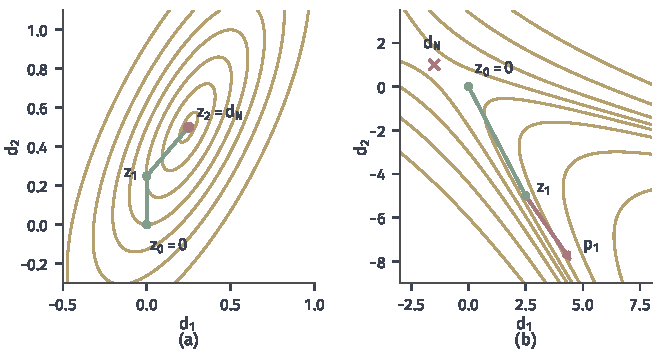
\includegraphics[width=112mm]{figures/05-optimization/02-smooth-optimization/matplotlib/newton-cg-truncation/figure.pdf}
  \caption{位移空间中的内层共轭梯度，黄线是局部模型的等高线。(a)在$(\tfrac12,0)$处模型是碗，绿色折线两步到达红点所示的Newton方向。(b)在$(-\tfrac12,\tfrac34)$处模型不定，绿线是第一步，红色箭头$\bm{p}_1$（按$0.05$倍绘制）是遇到的负曲率方向，内层在$\bm{z}_1$处停止；红叉是Newton方程的解，它是模型的鞍点。}
  \label{fig:newton-cg-truncation}
\end{BookInlineFigure}

\paragraph{与非线性共轭梯度的区别}
第~\ref{chap:first-order-methods}章的非线性共轭梯度法也叫共轭梯度，两者在做不同的事。

\begin{BookInlineTable}
  \centering
  \begin{tabular}{@{}lll@{}}
    \toprule
    & Newton-CG的内层 & 非线性共轭梯度法 \\
    \midrule
    作用对象 & 固定的二次模型 & 原目标 \\
    每步信息 & 一次$\bm{H}\bm{v}$ & 梯度和线搜索的函数值 \\
    步长 & 式~\eqref{eq:newton-cg-step}的闭式公式 & 线搜索 \\
    共轭性 & 模型上精确（不计舍入） & 一般只近似成立 \\
    有限步终止 & 不超过$n$步 & 没有此结论 \\
    \bottomrule
  \end{tabular}
  \caption{二次模型上的线性共轭梯度和直接作用于原目标的非线性共轭梯度。前者是一轮外层迭代中的线性方程求解器。}
  \label{tab:newton-cg-vs-ncg}
\end{BookInlineTable}

\paragraph{计算过程}
外层和内层的关系见图~\ref{fig:newton-cg-loops}。下面用目标~\eqref{eq:newton-running-objective}从Hessian不定的点$(-\tfrac12,\tfrac34)$出发。

\begin{BookInlineFigure}
  \centering
  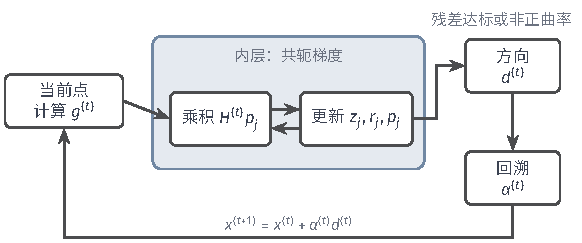
\includegraphics[width=99mm]{figures/05-optimization/02-smooth-optimization/tikz/newton-cg-loops/figure.pdf}
  \caption{Newton-CG的结构。外层读取梯度，内层只通过Hessian向量积与目标交互，在残差达到式~\eqref{eq:newton-inexact-condition}或遇到非正曲率时返回方向$\bm{d}^{(t)}$，外层再用回溯确定步长。}
  \label{fig:newton-cg-loops}
\end{BookInlineFigure}

\needspace{6\baselineskip}
\paragraph{变量}
\begin{itemize}
 \item $\bm{x},\bm{g}$：外层的当前点和梯度。
 \item $\eta_t$：本轮的误差比例。
 \item $\bm{z},\bm{r},\bm{p}$：内层的近似解、残差和搜索方向，每轮外层重新初始化。
 \item $\bm{q}$：工作向量，存放$\bm{H}\bm{p}$。
 \item $\bm{d},\alpha$：外层方向和步长。
 \item 不需要$\bm{H}$的存储，只需要计算$\bm{H}\bm{v}$的子程序。
\end{itemize}

\paragraph{初始化}
选定$\bm{x}^{(0)}$，$c$，$\beta$，$\varepsilon$。例中初始点和外层容差为
\[
 \bm{x}^{(0)}=\bigl(-\tfrac12,\tfrac34\bigr),\qquad c=0.1,\qquad \beta=0.5,\qquad \varepsilon=10^{-6}.
\]
误差比例取式~\eqref{eq:newton-forcing-rule}中的第一种，曲率阈值取$\epsilon=0$。

\needspace{6\baselineskip}
\paragraph{每轮更新}
在第$t$轮外层：
\begin{enumerate}
 \item \textbf{读取梯度并检查停止。}计算$\bm{g}^{(t)}$；若$\lVert\bm{g}^{(t)}\rVert_2\leq\varepsilon$，结束。然后确定$\eta_t$。

 例中第一轮$\bm{g}^{(0)}=(-\tfrac12,1)$，$\lVert\bm{g}^{(0)}\rVert_2=1.118$，$\eta_0=0.5$。

 \item \textbf{内层初始化。}令$\bm{z}_0=\bm{0}$，$\bm{r}_0=\bm{g}^{(t)}$，$\bm{p}_0=-\bm{g}^{(t)}$，$j=0$。

 \item \textbf{内层迭代。}计算$\bm{q}=\bm{H}^{(t)}\bm{p}_j$及曲率$\bm{p}_j^\top\bm{q}$。曲率不超过阈值时按式~\eqref{eq:newton-cg-truncate}返回方向。否则按式~\eqref{eq:newton-cg-step}更新；若$\bm{z}_{j+1}$已满足条件~\eqref{eq:newton-inexact-condition}，就返回它。否则按式~\eqref{eq:newton-cg-direction}更新方向，令$j\leftarrow j+1$。

 例中第一轮外层的第一步内层，$\bm{p}_0=(\tfrac12,-1)$，乘积和曲率为
 \[
  \bm{q}=\begin{bmatrix}-1.5\\-1\end{bmatrix},\qquad \bm{p}_0^\top\bm{q}=0.25>0.
 \]
 步长$\alpha_0=1.25/0.25=5$，更新后
 \[
  \bm{z}_1=\begin{bmatrix}2.5\\-5\end{bmatrix},\qquad \bm{r}_1=\begin{bmatrix}-8\\-4\end{bmatrix}.
 \]
 残差比例是$8.94/1.118=8$，大于$\eta_0$，继续。这个比例大于$1$，说明模型并不是碗。

 第二步内层，$\beta_0=80/1.25=64$，方向、乘积和曲率为
 \[
  \bm{p}_1=\begin{bmatrix}40\\-60\end{bmatrix},\qquad
  \bm{q}=\begin{bmatrix}-80\\-40\end{bmatrix},\qquad
  \bm{p}_1^\top\bm{q}=-800<0.
 \]
 遇到负曲率，由式~\eqref{eq:newton-cg-truncate}返回$\bm{d}^{(0)}=\bm{z}_1=(2.5,-5)$，内层用了$2$次Hessian向量积。

 \item \textbf{回溯并更新。}从$\alpha=1$开始按式~\eqref{eq:newton-armijo}回溯，然后更新$\bm{x}$，令$t\leftarrow t+1$。

 例中第一轮方向导数为$-6.25$。$\alpha=1$和$\tfrac12$的目标值分别是$68.56$和$5.379$，都被拒绝。$\alpha=\tfrac14$的新点是$(0.125,-0.5)$，目标值$0.6487$，低于右端$1.2188$，接受。

 第二轮$\bm{g}^{(1)}=(-0.6172,-1.0313)$，$\lVert\bm{g}^{(1)}\rVert_2=1.202$，$\eta_1=0.5$，Hessian为
 \[
  \bm{H}^{(1)}=\begin{bmatrix}3.1875&-0.5\\-0.5&2\end{bmatrix}.
 \]
 内层第一步的曲率是$2.7047$，$\alpha_0=1.4444/2.7047=0.5340$，于是
 \[
  \bm{z}_1=\begin{bmatrix}0.3296\\0.5507\end{bmatrix},\qquad \bm{r}_1=\begin{bmatrix}0.1581\\-0.0946\end{bmatrix}.
 \]
 残差比例$0.184/1.202=0.153\leq0.5$，内层结束，只用了一次乘积。完整步被接受。
\end{enumerate}

各轮结果见表~\ref{tab:newton-cg-run}。第$9$轮梯度范数低于容差，迭代结束，最终得到$\bm{x}^{(9)}\approx(1,1)$，整个过程用了$14$次Hessian向量积。可以看到比例收紧之前内层大多只走一步，$\eta_t$变小后内层把方程解到精确。

\begin{BookInlineTable}
  \centering
  \begin{tabular}{@{}ccccccc@{}}
    \toprule
    $t$ & $\bm{x}^{(t)}$ & $f$ & $\lVert\bm{g}^{(t)}\rVert_2$ & $\eta_t$ & $\bm{H}\bm{v}$次数 & $\alpha^{(t)}$ \\
    \midrule
    $0$ & $(-0.5,0.75)$ & $1.375$ & $1.118$ & $0.5$ & $2$（负曲率）& $1/4$ \\
    $1$ & $(0.125,-0.5)$ & $0.6487$ & $1.202$ & $0.5$ & $1$ & $1$ \\
    $2$ & $(0.4546,0.0507)$ & $0.1730$ & $0.407$ & $0.5$ & $1$ & $1$ \\
    $3$ & $(0.8099,0.4739)$ & $0.05121$ & $0.540$ & $0.5$ & $1$ & $1$ \\
    $4$ & $(0.7596,0.5197)$ & $0.03218$ & $0.132$ & $0.364$ & $2$ & $1$ \\
    $5$ & $(0.9552,0.8741)$ & $2.47\mathrm{e}{-3}$ & $0.127$ & $0.356$ & $1$ & $1$ \\
    $6$ & $(0.9448,0.8820)$ & $1.64\mathrm{e}{-3}$ & $0.0260$ & $0.161$ & $2$ & $1$ \\
    $7$ & $(0.9977,0.9927)$ & $1.04\mathrm{e}{-5}$ & $0.0105$ & $0.102$ & $2$ & $1$ \\
    $8$ & $(0.99998,0.99995)$ & $3.43\mathrm{e}{-10}$ & $1.13\mathrm{e}{-5}$ & $0.0034$ & $2$ & $1$ \\
    $9$ & $(1.0000,1.0000)$ & & $2.4\mathrm{e}{-9}$ & 停止 & & \\
    \bottomrule
  \end{tabular}
  \caption{Newton-CG在目标~\eqref{eq:newton-running-objective}上的运行，$\eta_t=\min\{0.5,\sqrt{\lVert\bm{g}^{(t)}\rVert_2}\}$。第$0$轮内层因负曲率提前结束。}
  \label{tab:newton-cg-run}
\end{BookInlineTable}

\paragraph{适用范围与补充}
非正曲率规则只保证方向可用，没有利用负曲率本身携带的信息。把遇到的$\bm{p}_j$当作离开鞍点的方向，或者在一个有限半径的区域内求解模型，分别是第~\ref{chap:saddle-points}章和第~\ref{chap:trust-region}章的内容。另外，CG只能看到由$\bm{g}^{(t)}$生成的Krylov子空间；若$\bm{g}^{(t)}$恰好与某个负曲率方向正交，CG也察觉不到它。

Hessian病态时，内层CG本身收敛很慢，这时可以预条件，做法与线性方程中的预条件共轭梯度法相同，见前面引用的Krylov一章。

\section{收敛与计算成本}
\label{sec:newton-cost}

前四节各解决了一个困难。于是要问：在同样的精度要求下，从起点走到终点，这些方法各要花多少计算，局部收敛快是否就意味着总成本低？

\paragraph{统一的比较口径}
沿用第~\ref{chap:smooth-foundations}章的口径：所有方法以$\lVert\bm{g}^{(t)}\rVert_2\leq\varepsilon$为停止标准，返回最后的迭代点，总成本是各轮成本之和。每轮的成本分三部分：读取目标和导数、线性代数运算、线搜索的函数计算。

记一次函数、梯度、Hessian、Hessian向量积的成本为$c_f,c_g,c_H,c_{Hv}$。对稠密问题，$c_{Hv}$约为$2n^2$次运算。表~\ref{tab:newton-cost-per-iter}按每轮的成本比较各方法，并把保障分开写。

\begin{BookInlineTable}
  \centering
  \small
  \begin{tabular}{@{}llll@{}}
    \toprule
    方法 & 每轮主要成本 & 远处的保障 & 近解行为 \\
    \midrule
    Newton法 & $c_H$，分解$\tfrac13n^3$ & 无 & 二次 \\
    阻尼Newton & 上述加回溯的$c_f$ & 正定时下降 & 接受整步后二次 \\
    对角平移 & $c_H$，分解可能重复若干次 & $\bm{g}\to\bm{0}$ & 修正消失后二次 \\
    谱修正 & $c_H$，特征分解 & $\bm{g}\to\bm{0}$ & 修正消失后二次 \\
    修正Cholesky & $c_H$，分解约$\tfrac13n^3$ & $\bm{g}\to\bm{0}$ & 修正消失后二次 \\
    Newton-CG & $k_tc_{Hv}$，无分解 & 方向下降，回溯 & 由$\eta_t$决定 \\
    \bottomrule
  \end{tabular}
  \caption{各方法单轮成本和收敛保障的比较，$k_t$是第$t$轮内层的Hessian向量积次数。“$\bm{g}\to\bm{0}$”需要定理~\ref{thm:newton-modified-global}的条件，“修正消失”要求解处Hessian正定且修正规则先试零修正。}
  \label{tab:newton-cost-per-iter}
\end{BookInlineTable}

\paragraph{两个阶段分开计算}
定理~\ref{thm:newton-damped-global}和定理~\ref{thm:newton-unit-step}给出阻尼Newton法的总步数上界。取强凸常数$\mu$、光滑常数$L$、Hessian的Lipschitz常数$M$和定理中的阈值$\tau$。

第一阶段是$\lVert\bm{g}^{(t)}\rVert_2>\tau$的轮次。由定理~\ref{thm:newton-damped-global}证明的第四步，每轮目标至少下降
\[
 \gamma=\frac{c\beta\tau^2}{\kappa L}.
\]
目标总下降量不超过$f(\bm{x}^{(0)})-f^\star$，所以这一阶段的轮数不超过$(f(\bm{x}^{(0)})-f^\star)/\gamma$。

第二阶段记$b_t=M\lVert\bm{g}^{(t)}\rVert_2/(2\mu^2)$，由式~\eqref{eq:newton-gradient-quadratic}，$b_{t+1}\leq b_t^2$，且起始时$b\leq\tfrac12$。要使$\lVert\bm{g}\rVert_2\leq\varepsilon$，只需$2^{-2^t}\leq M\varepsilon/(2\mu^2)$。于是总步数满足
\begin{equation}
 T\leq\frac{f(\bm{x}^{(0)})-f^\star}{\gamma}+\Bigl\lceil\log_2\log_2\frac{2\mu^2}{M\varepsilon}\Bigr\rceil.
 \label{eq:newton-total-iterations}
\end{equation}

第二项随精度增长极慢：$\varepsilon$从$10^{-6}$收紧到$10^{-12}$，只多大约一步。第一项与$\varepsilon$无关，却含有问题常数，通常主导总步数。所以局部收敛阶回答“到了解附近以后怎样”，全局成本回答“总共要花多少”，只看前者不足以判断整体效率。

\paragraph{贵的一步和便宜的很多步}
Newton法每轮贵，轮数少；一阶方法每轮便宜，轮数多。若梯度下降需要$T_{\mathrm{GD}}$轮，Newton法需要$T_{\mathrm{N}}$轮，分解成本记为$c_{\mathrm{fac}}$，则Newton法更划算的条件是
\begin{equation}
 T_{\mathrm{N}}\bigl(c_g+c_H+c_{\mathrm{fac}}\bigr)<T_{\mathrm{GD}}\,c_g.
 \label{eq:newton-breakeven}
\end{equation}

主例从$(\tfrac12,0)$出发，把梯度范数降到$10^{-6}$，回溯梯度下降用了$245$轮、$792$次函数计算，Newton法用了$5$轮。二维问题的分解几乎不花时间，所以Newton法的总成本低得多。

规模变大，结论就可能相反。取稠密$n=10^4$，一次Cholesky分解约$3.3\times10^{11}$次运算，一次梯度若与$n^2$同量级，一次分解约相当于$1700$次矩阵向量乘积。若不到一千次梯度步就能达到要求的精度，Newton法在稠密实现下就不划算。反过来，Hessian稀疏时分解可能很便宜，三对角矩阵的分解只需$O(n)$次运算。比较时必须用实际的结构，不能只看$n$。

\paragraph{内层的精度也要计入成本}
非精确方法的比较要把内层计入。取式~\eqref{eq:newton-running-objective}的链式推广，$n=1000$：
\begin{equation}
 f(\bm{x})=\sum_{i=1}^{n-1}\Bigl[\frac12(x_i-1)^2+(x_{i+1}-x_i^2)^2\Bigr].
 \label{eq:newton-chain-objective}
\end{equation}
从分量交替取$-1.2$和$1$的点出发，用带回溯（$c=10^{-4}$）的Newton-CG，把梯度范数降到$10^{-9}$。结果列在表~\ref{tab:newton-cg-cost}中，图~\ref{fig:newton-cost}画出了全过程。

\begin{BookInlineTable}
  \centering
  \begin{tabular}{@{}lcc@{}}
    \toprule
    误差比例 & 外层轮数 & $\bm{H}\bm{v}$总次数 \\
    \midrule
    $\eta=0.5$ & $29$ & $93$ \\
    $\eta=0.1$ & $15$ & $72$ \\
    $\eta_t=\min\{0.5,\sqrt{\lVert\bm{g}^{(t)}\rVert_2}\}$ & $17$ & $100$ \\
    $\eta=10^{-10}$（近乎精确求解） & $12$ & $357$ \\
    \bottomrule
  \end{tabular}
  \caption{目标~\eqref{eq:newton-chain-objective}上不同误差比例的成本。内层解得越精确，外层轮数越少，总乘积次数却可能大幅增加。}
  \label{tab:newton-cg-cost}
\end{BookInlineTable}

\begin{BookInlineFigure}
  \centering
  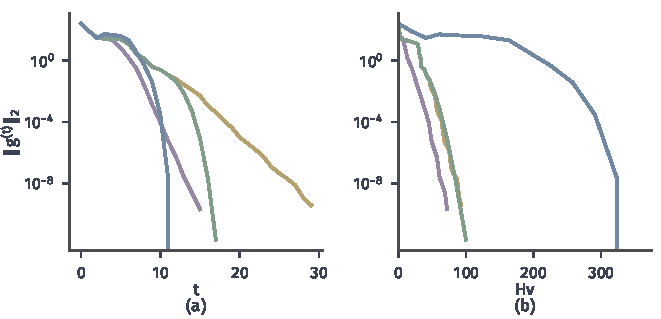
\includegraphics[width=112mm]{figures/05-optimization/02-smooth-optimization/matplotlib/newton-cost/figure.pdf}
  \caption{目标~\eqref{eq:newton-chain-objective}上Newton-CG的进展，$n=1000$。(a)梯度范数随外层轮数$t$的变化，(b)随累计Hessian向量积次数的变化。黄线$\eta=0.5$，紫线$\eta=0.1$，绿线$\eta_t=\min\{0.5,\sqrt{\lVert\bm{g}^{(t)}\rVert_2}\}$，蓝线$\eta=10^{-10}$。蓝线在(a)中外层轮数最少，在(b)中总成本最高。}
  \label{fig:newton-cost}
\end{BookInlineFigure}

这组数据说明两点。第一，把内层解到接近精确，与$\eta=0.1$相比外层只少了三轮，乘积次数却是它的五倍。第二，表中自适应规则的乘积次数并不最少，$\eta=0.1$在这个例子上反而更好。自适应规则的好处是不需要调参并且保证局部快速收敛，而不是在每个问题上都最省。

还要注意目标~\eqref{eq:newton-chain-objective}的Hessian是三对角的，稀疏Cholesky分解每次只要$O(n)$次运算，这种情况下精确Newton法也相当便宜。Newton-CG的优势主要在Hessian稠密、结构不便分解、或者根本不想形成矩阵的时候。

\paragraph{三种手段的组合}
阻尼、修正、非精确求解作用在迭代的不同环节，可以按需要组合。实际程序中常见的组合是：Hessian可以分解时，用试探$\delta$的修正Cholesky或对角平移加回溯；规模太大时，用Newton-CG加回溯，负曲率时截断。每一种组合的保证都要对应地核对：下降方向由哪一环保证，步长由哪一环保证，局部速度又由哪些量趋于零来保证。

\section{本章小结}
\label{sec:newton-summary}

Newton法把优化问题变成一串线性方程：在当前点用二次模型代替目标，解$\bm{H}^{(t)}\bm{d}^{(t)}=-\bm{g}^{(t)}$，走到模型的极小点。Hessian正定时这个方向下降；解处非退化、Hessian Lipschitz且初始点足够近时，收敛是二次的。

完整的Newton步在其余情形下都可能出问题。本章把困难分成三类，每一类用一个独立的量来控制，如图~\ref{fig:newton-three-controls}所示。

\begin{BookInlineFigure}
  \centering
  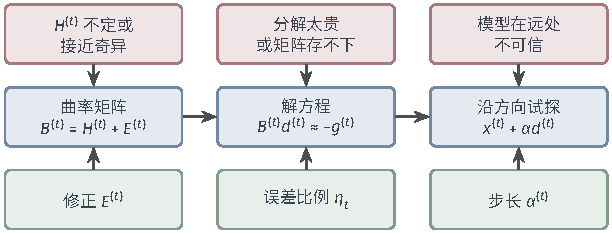
\includegraphics[width=104mm]{figures/05-optimization/02-smooth-optimization/tikz/newton-three-controls/figure.pdf}
  \caption{本章三种手段的分工。上行是遇到的困难，中行是迭代中受影响的环节，下行是对应的控制量。三个控制量互相独立，可以单独使用，也可以组合。}
  \label{fig:newton-three-controls}
\end{BookInlineFigure}

阻尼不改方向，只选步长$\alpha^{(t)}\leq1$，靠原目标的下降检验保证进展。强凸时全局线性收敛，梯度足够小后完整步自动恢复，局部二次收敛得以保留。

修正改变曲率矩阵，用$\bm{H}^{(t)}+\bm{E}^{(t)}$代替Hessian。对角平移、谱修正和修正Cholesky分解在修正量和计算量之间取舍。修正量一致有界时梯度趋于零，极限点可能是鞍点；修正消失后恢复Newton的局部行为。

非精确求解放宽线性方程，用残差比例$\eta_t$规定内层精度。比例保持小于$1$得到线性收敛，趋于零得到超线性收敛，与梯度同阶得到二次收敛。Newton-CG只用Hessian向量积，遇到非正曲率截断，方向总是下降的。

比较成本时要把外层轮数和内层工作一起计入，把远离解时的保障与解附近的速度分开看。局部收敛阶说明最后几步，总成本还取决于第一阶段的轮数和每轮的实际代价。

这些方法都要求能读取Hessian或它与向量的乘积。下一章研究不直接计算Hessian时，怎样从相邻两次梯度的变化中构造可用的曲率近似。


\chapter{拟牛顿法}
\label{chap:quasi-newton}

假设目标有$n=10^4$个变量，算一次梯度只需几毫秒。第~\ref{chap:second-order-methods}章的Newton法收敛很快，但它每一步都要形成Hessian，保存约$5\times10^7$个不同的元素，再做一次约$3\times10^{11}$次运算的分解。第~\ref{chap:first-order-methods}章的梯度下降每步只需要梯度，可是在狭长的山谷里它不断来回折返，因为它完全不知道地形朝哪个方向弯得厉害。

这两者之间有一个常被浪费的信息来源。迭代走了一步之后，我们手里有相邻两点的梯度，两个梯度的差反映了这一段路上地形的弯曲。这件事不需要额外的计算，只要把数字留下来。

本章研究怎样把这些“免费”的曲率测量攒成一个可用的矩阵。第~\ref{sec:qn-secant}节写出测量给出的条件，并说明为什么单靠它定不出矩阵。第~\ref{sec:qn-dfp-bfgs}节用两个秩一项做修正，得到DFP和BFGS两种更新，重点在怎样保持矩阵正定。

第~\ref{sec:qn-sr1}节只用一个秩一项，它能记住负曲率，代价是失去正定性。第~\ref{sec:qn-lbfgs}节处理连$n\times n$矩阵都存不下的情形，只保留最近几次测量。第~\ref{sec:qn-convergence}节在同一套条件下逐个核对这些方法能保证什么，并按相同精度比较计算成本。

全章用同一个二维目标做手算：
\begin{equation}
 f(\bm{x})=x_1^2+4x_2^2,\qquad \bm{x}^{(0)}=(4,1)^\top.
 \label{eq:qn-running-example}
\end{equation}
它的Hessian是$\bm{A}=\operatorname{diag}(2,8)$，最优解是原点。算法并不知道$\bm{A}$，它只能在迭代点上读取梯度$\nabla f(\bm{x})=\bm{A}\bm{x}$。

\section{割线条件}
\label{sec:qn-secant}

不计算Hessian，单凭已经读到的梯度，能知道多少曲率？答案是一条线性方程组，它精确地说出了一次测量包含的信息，也说明了这些信息还远远不够。

\paragraph{用近似矩阵代替Hessian}
Newton法在当前点$\bm{x}^{(t)}$处用二次模型近似目标。把模型里的Hessian换成一个对称矩阵$\bm{B}^{(t)}$，模型变成
\begin{equation}
 m^{(t)}(\bm{p})=f(\bm{x}^{(t)})+\langle\bm{g}^{(t)},\bm{p}\rangle+\frac12\bm{p}^\top\bm{B}^{(t)}\bm{p}.
 \label{eq:qn-model}
\end{equation}
当$\bm{B}^{(t)}$正定时，模型是严格凸的，令它的梯度$\bm{g}^{(t)}+\bm{B}^{(t)}\bm{p}$为零，得到唯一极小点
\begin{equation}
 \bm{d}^{(t)}=-\bm{W}^{(t)}\bm{g}^{(t)},\qquad\bm{W}^{(t)}=\bigl(\bm{B}^{(t)}\bigr)^{-1}.
 \label{eq:qn-direction}
\end{equation}
这里$\bm{B}^{(t)}$叫曲率近似，$\bm{W}^{(t)}$叫逆曲率近似。全卷$\bm{H}^{(t)}$专指真实Hessian，所以逆近似用$\bm{W}$表示。下面只需要回答一件事：这两个矩阵从哪里来。

\paragraph{一维情形：割线}
先看只有一个变量的目标。设$f(x)=\tfrac14x^4+\tfrac12x^2$，梯度$g(x)=x^3+x$，已经走过$x^{(0)}=1$和$x^{(1)}=0.5$，读到
\[
 g(x^{(0)})=2,\qquad g(x^{(1)})=0.625.
\]
过这两点作$g$的割线，斜率是
\[
 b=\frac{g(x^{(1)})-g(x^{(0)})}{x^{(1)}-x^{(0)}}=\frac{0.625-2}{0.5-1}=2.75.
\]

这个斜率介于两端的真实二阶导数$f''(0.5)=1.75$与$f''(1)=4$之间。由微积分基本定理，它正好是$f''$在这一段上的平均值。把$b$当作曲率，下一个点就是割线与横轴的交点：
\[
 x^{(2)}=x^{(1)}-\frac{g(x^{(1)})}{b}=0.5-\frac{0.625}{2.75}\approx0.273.
\]
图~\ref{fig:qn-secant-1d}画出了这一步。割线不如切线精确，却不需要二阶导数，只用两次已经算过的梯度。

\begin{BookInlineFigure}
  \centering
  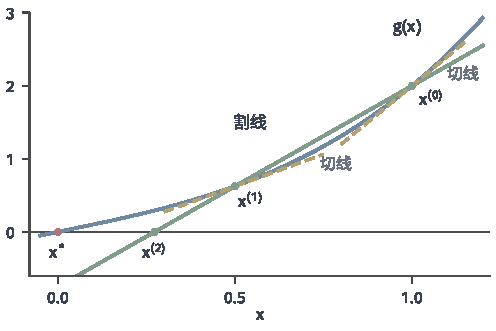
\includegraphics[width=84mm]{figures/05-optimization/02-smooth-optimization/matplotlib/qn-secant-1d/figure.pdf}
  \caption{一维的割线步。蓝线是$f(x)=\tfrac14x^4+\tfrac12x^2$的梯度$g(x)=x^3+x$。绿线是过$x^{(0)}=1$、$x^{(1)}=0.5$两点的割线，斜率$2.75$是$f''$在这一段的平均值；两条黄色虚线是两端的切线，斜率分别为$4$和$1.75$。割线与横轴的交点给出下一个迭代点$x^{(2)}\approx0.273$，红点是最优解。}
  \label{fig:qn-secant-1d}
\end{BookInlineFigure}

\paragraph{高维情形：梯度差是平均曲率作用于位移}
高维时除法做不了，但关系仍在。记位移与梯度差分别为
\begin{equation}
 \bm{s}^{(t)}=\bm{x}^{(t+1)}-\bm{x}^{(t)},\qquad\bm{y}^{(t)}=\bm{g}^{(t+1)}-\bm{g}^{(t)}.
 \label{eq:qn-s-y}
\end{equation}
沿线段$\bm{x}^{(t)}+\tau\bm{s}^{(t)}$（$\tau\in[0,1]$）对梯度用微积分基本定理，得到
\begin{equation}
 \bm{y}^{(t)}=\bar{\bm{H}}^{(t)}\bm{s}^{(t)},\qquad
 \bar{\bm{H}}^{(t)}=\int_0^1\nabla^2f\bigl(\bm{x}^{(t)}+\tau\bm{s}^{(t)}\bigr)\,\mathrm{d}\tau.
 \label{eq:qn-average-hessian}
\end{equation}
所以$\bm{y}^{(t)}$是这一段路上的平均Hessian作用在位移上的结果。对二次目标，Hessian是常数$\bm{A}$，等式成为精确的$\bm{y}^{(t)}=\bm{A}\bm{s}^{(t)}$。

可以把每一步想成一次路试。车沿某条路开过去，记下坡度的变化，就知道这条路上地形弯得多厉害。对应关系是：路线对应$\bm{s}^{(t)}$，坡度变化对应$\bm{y}^{(t)}$，弯曲程度对应$\bar{\bm{H}}^{(t)}$在这个方向上的作用。

这个类比有两处要小心。一次路试只告诉我们沿路线方向的信息，与路线垂直的方向几乎没有测量；地形不是二次的时候，旧路试测到的曲率会随着位置改变而过时。

既然模型要代表目标在下一个点的局部形状，自然要求新的矩阵重现最新的测量。

\begin{definition}[割线条件]
\label{def:qn-secant}
给定$\bm{s}^{(t)}$与$\bm{y}^{(t)}$，称对称矩阵$\bm{B}^{(t+1)}$满足\term{割线条件}（secant condition），如果
\begin{equation}
 \bm{B}^{(t+1)}\bm{s}^{(t)}=\bm{y}^{(t)}.
 \label{eq:qn-secant}
\end{equation}
用逆曲率近似$\bm{W}^{(t+1)}$表示时，条件写成
\begin{equation}
 \bm{W}^{(t+1)}\bm{y}^{(t)}=\bm{s}^{(t)}.
 \label{eq:qn-secant-inverse}
\end{equation}
\end{definition}

割线条件有一个几何含义。以$\bm{x}^{(t+1)}$为中心的模型在新点的梯度是$\bm{g}^{(t+1)}$，在旧点（$\bm{p}=-\bm{s}^{(t)}$）的梯度是
\[
 \bm{g}^{(t+1)}-\bm{B}^{(t+1)}\bm{s}^{(t)}=\bm{g}^{(t+1)}-\bm{y}^{(t)}=\bm{g}^{(t)}.
\]
也就是说，模型在新旧两点的梯度都与目标一致。使用满足割线条件的矩阵，并按这种方式选择方向的方法统称\term{拟牛顿法}（quasi-Newton method）。

下面用贯穿例算出第一组测量。取$\bm{W}^{(0)}=\bm{I}$，第一步就是负梯度方向。在二次目标上，沿方向$\bm{d}$的精确线搜索步长是
\[
 \alpha=\frac{-\langle\bm{g},\bm{d}\rangle}{\bm{d}^\top\bm{A}\bm{d}}.
\]
代入第一轮的数据，得到
\[
 \bm{g}^{(0)}=(8,8)^\top,\qquad\bm{d}^{(0)}=(-8,-8)^\top,\qquad\alpha^{(0)}=\frac{128}{640}=\frac15.
\]

走完这一步，得到新的点和梯度：
\[
 \bm{x}^{(1)}=(2.4,-0.6)^\top,\qquad\bm{g}^{(1)}=(4.8,-4.8)^\top.
\]
位移和梯度差是
\begin{equation}
 \bm{s}^{(0)}=(-1.6,-1.6)^\top,\qquad\bm{y}^{(0)}=(-3.2,-12.8)^\top.
 \label{eq:qn-running-pair}
\end{equation}

\paragraph{一条割线条件定不出矩阵}
割线条件有$n$个方程，对称矩阵有$n(n+1)/2$个自由元素，还差$n(n-1)/2$个条件。$n=1$时恰好相等，这正是一维割线法没有选择余地的原因。$n$一大，缺口迅速变大。

图~\ref{fig:qn-secant-unknowns}说明缺的是哪些信息。把$\bm{s}$单位化后作为第一个基向量。$\bm{B}\bm{s}=\bm{y}$确定了矩阵的第一列，对称性再确定第一行，其余$(n-1)\times(n-1)$的对称块完全自由。换句话说，矩阵在与$\bm{s}$正交的子空间内怎样弯曲，这次路试没有提供任何信息。

\begin{BookInlineFigure}
  \centering
  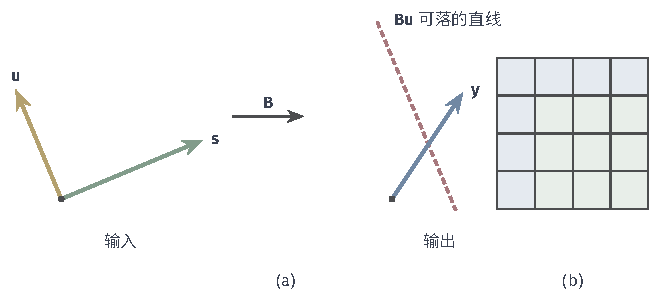
\includegraphics[width=110mm]{figures/05-optimization/02-smooth-optimization/tikz/qn-secant-unknowns/figure.pdf}
  \caption{割线条件确定了矩阵的哪些部分。(a)$n=2$时，$\bm{B}$把$\bm{s}$送到已知的$\bm{y}$；对另一个方向$\bm{u}$，对称性只给出$\langle\bm{Bu},\bm{s}\rangle=\langle\bm{u},\bm{y}\rangle$，所以$\bm{Bu}$只知道落在红色虚线上。(b)$n=4$时，在以$\bm{s}$为第一个基向量的正交基下，蓝色的第一行第一列由割线条件和对称性确定，绿色的$3\times3$对称块的$6$个元素仍然自由。}
  \label{fig:qn-secant-unknowns}
\end{BookInlineFigure}

用贯穿例看得更具体。设$\bm{B}=\begin{bmatrix}a&b\\b&c\end{bmatrix}$，把式~\eqref{eq:qn-running-pair}代入割线条件，两个方程约去公因子后是
\[
 a+b=2,\qquad b+c=8.
\]
三个未知数、两个方程，还剩一个自由参数：
\begin{equation}
 \bm{B}(a)=\begin{bmatrix}a&2-a\\2-a&6+a\end{bmatrix},\qquad
 \det\bm{B}(a)=10a-4.
 \label{eq:qn-secant-family}
\end{equation}
真实Hessian是其中$a=2$的成员，但算法无从知道。

族中不同成员给出的方向也不同。若第一步取较短的步长$\alpha^{(0)}=1/8$，位移与梯度差只差一个倍数，方程不变，于是仍是族~\eqref{eq:qn-secant-family}。此时$\bm{x}^{(1)}=(3,0)^\top$，$\bm{g}^{(1)}=(6,0)^\top$，方向$-\bm{B}(a)^{-1}\bm{g}^{(1)}$的计算结果是
\[
 \begin{aligned}
 a=0.9:&\quad(-8.28,\ 1.32)^\top,\\
 a=2:&\quad(-3,\ 0)^\top,\\
 a=5:&\quad(-1.435,\ -0.391)^\top.
 \end{aligned}
\]

只有$a=2$的方向一步落到最优解。图~\ref{fig:qn-secant-family}(a)把这些模型画在一起：它们在$\bm{x}^{(0)}$处都与同一条红色切线相切，这是割线条件保证的，在别的地方却差别很大，极小点也各不相同。

\begin{BookInlineFigure}
  \centering
  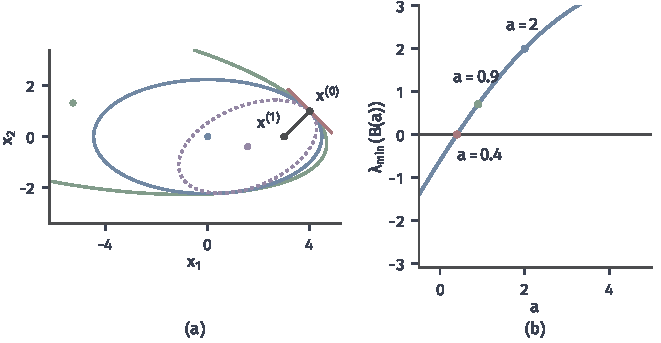
\includegraphics[width=112mm]{figures/05-optimization/02-smooth-optimization/matplotlib/qn-secant-family/figure.pdf}
  \caption{满足同一割线条件的矩阵族~\eqref{eq:qn-secant-family}。(a)从$\bm{x}^{(0)}=(4,1)$走到$\bm{x}^{(1)}=(3,0)$后，$a=0.9$（绿）、$a=2$（蓝）、$a=5$（紫，点线）三个模型过$\bm{x}^{(0)}$的等值线，它们在$\bm{x}^{(0)}$处有同一条切线（红），同色小点是各模型的极小点。(b)$\bm{B}(a)$的最小特征值，$a>0.4$时为正。}
  \label{fig:qn-secant-family}
\end{BookInlineFigure}

\paragraph{还要补充什么要求}
既然割线条件不够，就要额外规定想要什么样的矩阵。后面各种方法的区别，就在这些补充要求上。

第一是\textbf{对称}。Hessian对称，近似矩阵也应该对称，这已经写进了定义。

第二是\textbf{低秩修正}：$\bm{B}^{(t+1)}$与$\bm{B}^{(t)}$只差一个秩很低的矩阵。这样做既保留了以前路试积累的信息，也使更新只花$O(n^2)$次运算。它还能配合逆矩阵的公式，直接更新$\bm{W}$，于是根本不用解线性方程。

第三是\textbf{曲率性质}。我们希望$\bm{B}^{(t+1)}$正定，这样方向~\eqref{eq:qn-direction}才是模型的极小点。但正定性对测量数据有要求。用$\bm{s}^{(t)}$与割线条件~\eqref{eq:qn-secant}作内积，得到
\begin{equation}
 \bigl(\bm{s}^{(t)}\bigr)^\top\bm{B}^{(t+1)}\bm{s}^{(t)}=\langle\bm{s}^{(t)},\bm{y}^{(t)}\rangle.
 \label{eq:qn-curvature-identity}
\end{equation}
左边在$\bm{B}^{(t+1)}\succ\bm{0}$且$\bm{s}^{(t)}\neq\bm{0}$时为正，所以必须有
\begin{equation}
 \langle\bm{s}^{(t)},\bm{y}^{(t)}\rangle>0.
 \label{eq:qn-curvature-condition}
\end{equation}
这个不等式称为\term{曲率条件}（curvature condition）。它的含义是：沿刚走过的路，平均来看地形向上弯。

曲率条件确实可能不成立。取不定的二次目标，其Hessian为$\operatorname{diag}(2,-1)$，$\bm{s}=(1,2)^\top$，则
\[
 \bm{y}=(2,-2)^\top,\qquad\langle\bm{s},\bm{y}\rangle=2-4=-2<0.
\]
这时任何满足割线条件的矩阵都不可能正定。曲率条件是必要条件，第~\ref{sec:qn-dfp-bfgs}节将说明，配合恰当的更新，它也是充分的。

\paragraph{接入线搜索}
得到$\bm{W}^{(t)}$后，拟牛顿法沿用第~\ref{chap:smooth-foundations}章的线搜索框架：
\begin{equation}
 \bm{x}^{(t+1)}=\bm{x}^{(t)}+\alpha^{(t)}\bm{d}^{(t)},\qquad\bm{d}^{(t)}=-\bm{W}^{(t)}\bm{g}^{(t)}.
 \label{eq:qn-iteration}
\end{equation}
只要$\bm{W}^{(t)}$正定且$\bm{g}^{(t)}\neq\bm{0}$，就有
\[
 \langle\bm{g}^{(t)},\bm{d}^{(t)}\rangle=-\bigl(\bm{g}^{(t)}\bigr)^\top\bm{W}^{(t)}\bm{g}^{(t)}<0,
\]
方向是下降方向，线搜索一定能找到使目标下降的步长。

步长的试探从$\alpha=1$开始，因为$\bm{d}^{(t)}$本身是模型的极小点，近似矩阵好的时候它就是合适的长度。常用的接受标准是Wolfe条件：取$0<c_1<c_2<1$，要求$\alpha$同时满足充分下降和曲率两条不等式，
\begin{equation}
 \begin{aligned}
 f(\bm{x}^{(t)}+\alpha\bm{d}^{(t)})&\leq f(\bm{x}^{(t)})+c_1\alpha\langle\bm{g}^{(t)},\bm{d}^{(t)}\rangle,\\
 \langle\nabla f(\bm{x}^{(t)}+\alpha\bm{d}^{(t)}),\bm{d}^{(t)}\rangle&\geq c_2\langle\bm{g}^{(t)},\bm{d}^{(t)}\rangle.
 \end{aligned}
 \label{eq:qn-wolfe}
\end{equation}
第一条不让步长过长，第二条不让步长过短。第~\ref{chap:smooth-foundations}章已经说明，下降方向上目标有下界时，这样的步长总是存在。第二条在这里还有一个专门的用途，下一节会看到。

把三类方向放在一起，能看清拟牛顿法的位置。它们的区别不在迭代的形式，而在第一项的矩阵由什么信息构成。

\begin{BookInlineTable}
  \centering
  \begin{tabular}{llll}
    \toprule
    方法 & 方向 & 用到的信息 & 每步新增的曲率信息\\
    \midrule
    梯度下降 & $-\bm{g}^{(t)}$ & 梯度 & 无\\
    拟牛顿法 & $-\bm{W}^{(t)}\bm{g}^{(t)}$ & 梯度与历史 & 一次沿位移的测量\\
    Newton法 & $-(\bm{H}^{(t)})^{-1}\bm{g}^{(t)}$ & 梯度与Hessian & 完整的曲率\\
    \bottomrule
  \end{tabular}
  \caption{三类方向的对比。}
  \label{tab:qn-direction-comparison}
\end{BookInlineTable}

\section{DFP与BFGS}
\label{sec:qn-dfp-bfgs}

割线条件留下了很大的自由度。接下来要弄清：怎样用尽量小的对称修正满足它，同时让矩阵保持正定？答案是两个秩一项之和，改动的对象不同，就得到DFP和BFGS两种更新。

讨论一次更新时省略迭代上标：当前矩阵写作$\bm{B}$、$\bm{W}$，新矩阵写作$\bm{B}^{+}$、$\bm{W}^{+}$，位移和梯度差写作$\bm{s}$、$\bm{y}$，并记
\begin{equation}
 \rho=\frac{1}{\langle\bm{s},\bm{y}\rangle}.
 \label{eq:qn-rho}
\end{equation}

\paragraph{主要思想：秩二修正}
设新矩阵是旧矩阵加上两个对称秩一项：
\[
 \bm{B}^{+}=\bm{B}+a\bm{u}\bm{u}^\top+b\bm{v}\bm{v}^\top.
\]
代入割线条件$\bm{B}^{+}\bm{s}=\bm{y}$，得到
\[
 \bm{B}\bm{s}+a\langle\bm{u},\bm{s}\rangle\bm{u}+b\langle\bm{v},\bm{s}\rangle\bm{v}=\bm{y}.
\]

这个等式左边有三个向量，右边是$\bm{y}$。最直接的配法是让新增的一项产生$\bm{y}$，另一项抵消$\bm{B}\bm{s}$，也就是取$\bm{u}=\bm{y}$，$\bm{v}=\bm{B}\bm{s}$，并令
\[
 a\langle\bm{y},\bm{s}\rangle=1,\qquad b\,\bm{s}^\top\bm{B}\bm{s}=-1.
\]
由此得到\term{BFGS更新}（BFGS update）：
\begin{equation}
 \bm{B}^{+}=\bm{B}-\frac{\bm{B}\bm{s}\bm{s}^\top\bm{B}}{\bm{s}^\top\bm{B}\bm{s}}+\rho\,\bm{y}\bm{y}^\top.
 \label{eq:qn-bfgs-direct}
\end{equation}
名称取自Broyden、Fletcher、Goldfarb和Shanno四人。

更新的两项各做一件事。把旧矩阵减去第一项后的结果记为
\[
 \bm{P}=\bm{B}-\frac{\bm{B}\bm{s}\bm{s}^\top\bm{B}}{\bm{s}^\top\bm{B}\bm{s}}.
\]
它满足$\bm{P}\bm{s}=\bm{0}$，也就是把旧矩阵沿$\bm{s}$的曲率清空了。第二项把新测到的曲率填回去，因为$\rho\,\bm{y}\bm{y}^\top\bm{s}=\bm{y}$。

图~\ref{fig:qn-bfgs-strip}按贯穿例的第一次更新画出这个过程。旧矩阵的单位等值线是圆；清空沿$\bm{s}$的曲率之后，它变成沿$\bm{s}$无限延伸的带；加上测量项后，带又合拢成椭圆，形状已经向真实Hessian靠拢。

\begin{BookInlineFigure}
  \centering
  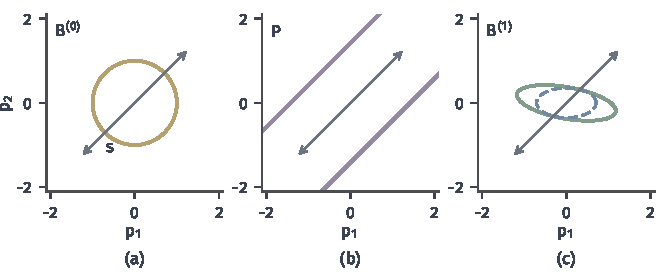
\includegraphics[width=112mm]{figures/05-optimization/02-smooth-optimization/matplotlib/qn-bfgs-strip/figure.pdf}
  \caption{贯穿例第一次BFGS更新的两步，曲线都是集合$\{\bm{p}:\bm{p}^\top\bm{M}\bm{p}=1\}$，箭头是$\bm{s}^{(0)}$所在的直线。(a)$\bm{M}=\bm{B}^{(0)}=\bm{I}$。(b)$\bm{M}=\bm{P}$，沿$\bm{s}$的曲率被清空，等值线变成平行的两条直线（紫）。(c)$\bm{M}=\bm{B}^{(1)}$（绿），加上测量项后重新合拢；蓝色虚线是真实Hessian的等值线。}
  \label{fig:qn-bfgs-strip}
\end{BookInlineFigure}

\paragraph{主要思想：对偶的DFP}
把同样的推导用在逆矩阵上。设$\bm{W}^{+}$是$\bm{W}$加上两个对称秩一项，代入割线条件~\eqref{eq:qn-secant-inverse}，取一项产生$\bm{s}$，另一项抵消$\bm{W}\bm{y}$，得到\term{DFP更新}（DFP update）：
\begin{equation}
 \bm{W}^{+}=\bm{W}-\frac{\bm{W}\bm{y}\bm{y}^\top\bm{W}}{\bm{y}^\top\bm{W}\bm{y}}+\rho\,\bm{s}\bm{s}^\top.
 \label{eq:qn-dfp-inverse}
\end{equation}
名称取自Davidon、Fletcher和Powell三人。对比式~\eqref{eq:qn-bfgs-direct}，两者互为对偶：在一个公式里交换$\bm{B}\leftrightarrow\bm{W}$、$\bm{s}\leftrightarrow\bm{y}$，就得到另一个。

实际计算只需要$\bm{W}$，方向~\eqref{eq:qn-direction}才不用解方程。DFP本来就是$\bm{W}$的公式，BFGS却要从$\bm{B}$翻译过来。下面的定理给出翻译的结果。

\begin{theorem}[BFGS的逆形式]
\label{thm:qn-bfgs-inverse}
设$\bm{B}\succ\bm{0}$，$\bm{W}=\bm{B}^{-1}$，$\bm{s}\neq\bm{0}$，$\langle\bm{s},\bm{y}\rangle>0$，并记$\bm{V}=\bm{I}-\rho\,\bm{y}\bm{s}^\top$。则式~\eqref{eq:qn-bfgs-direct}的$\bm{B}^{+}$可逆，其逆是
\begin{equation}
 \bm{W}^{+}=\bm{V}^\top\bm{W}\bm{V}+\rho\,\bm{s}\bm{s}^\top.
 \label{eq:qn-bfgs-inverse}
\end{equation}
\end{theorem}

\begin{proof}
只需验证$\bm{B}^{+}\bm{W}^{+}=\bm{I}$。先处理$\bm{B}^{+}\bm{V}^\top$。因为$\bm{V}^\top=\bm{I}-\rho\,\bm{s}\bm{y}^\top$，且$\bm{B}^{+}\bm{s}=\bm{y}$，所以
\[
 \bm{B}^{+}\bm{V}^\top=\bm{B}^{+}-\rho\,\bm{y}\bm{y}^\top=\bm{P}.
\]

再乘$\bm{W}$，由$\bm{B}\bm{W}=\bm{I}$，得到
\[
 \bm{P}\bm{W}=\bm{I}-\frac{\bm{B}\bm{s}\bm{s}^\top}{\bm{s}^\top\bm{B}\bm{s}}.
\]

接着由$\rho$的定义计算$\bm{s}^\top\bm{V}$：
\[
 \bm{s}^\top\bm{V}=\bm{s}^\top-\rho\langle\bm{s},\bm{y}\rangle\bm{s}^\top=\bm{0}^\top.
\]

所以右乘$\bm{V}$时第二项消失：
\[
 \bm{P}\bm{W}\bm{V}=\bm{V}.
\]

最后合并$\bm{W}^{+}$的两部分，并再用一次$\bm{B}^{+}\bm{s}=\bm{y}$：
\[
 \bm{B}^{+}\bm{W}^{+}=\bm{P}\bm{W}\bm{V}+\rho\,\bm{B}^{+}\bm{s}\bm{s}^\top=\bm{V}+\rho\,\bm{y}\bm{s}^\top=\bm{I}.
\]
方阵有右逆即可逆，定理得证。
\end{proof}

同样的公式也可以两次使用Sherman--Morrison公式得到，秩一修正求逆的公式可参考\BookChapterRef{chap:direct-linear-solvers}{卷二第12章“线性方程的直接求解”}。对偶地，DFP的直接形式是
\begin{equation}
 \bm{B}^{+}=\bm{V}\bm{B}\bm{V}^\top+\rho\,\bm{y}\bm{y}^\top.
 \label{eq:qn-dfp-direct}
\end{equation}

\paragraph{主要思想：新测量取代旧记忆}
逆形式~\eqref{eq:qn-bfgs-inverse}有一个清楚的解释。任取向量$\bm{z}$，令$a=\rho\langle\bm{s},\bm{z}\rangle$，由$\bm{V}$的定义，
\begin{equation}
 \bm{z}=a\,\bm{y}+\bm{V}\bm{z},\qquad\langle\bm{s},\bm{V}\bm{z}\rangle=0.
 \label{eq:qn-z-decomposition}
\end{equation}
也就是说，$\bm{z}$被拆成沿$\bm{y}$的部分和与$\bm{s}$正交的部分（这个拆分不是正交分解）。

把$\bm{W}^{+}$作用到$\bm{z}$上，得到
\[
 \bm{W}^{+}\bm{z}=a\,\bm{s}+\bm{V}^\top\bm{W}\bm{V}\bm{z}.
\]
沿$\bm{y}$的部分直接按测量结果换成$\bm{s}$，这正是割线条件；其余部分仍用旧矩阵$\bm{W}$处理，只是最后用$\bm{V}^\top$投影到$\bm{y}$的正交补上。图~\ref{fig:qn-bfgs-decomposition}画出了这个分解。

\begin{BookInlineFigure}
  \centering
  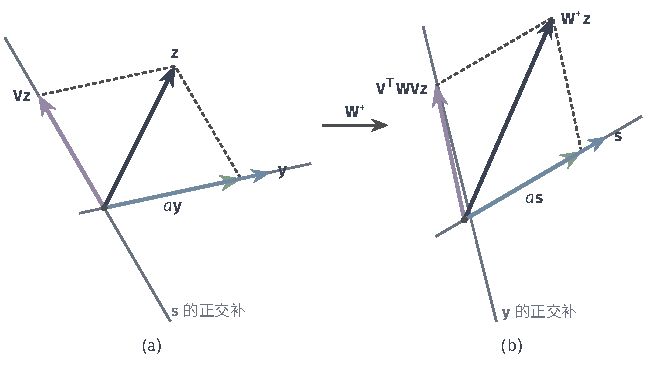
\includegraphics[width=108mm]{figures/05-optimization/02-smooth-optimization/tikz/qn-bfgs-decomposition/figure.pdf}
  \caption{BFGS逆更新对向量$\bm{z}$的作用，示意中旧矩阵取$\bm{W}=\bm{I}$。(a)$\bm{z}$沿$\bm{y}$与$\bm{s}$的正交补拆成两部分。(b)沿$\bm{y}$的部分$a\bm{y}$被换成$a\bm{s}$（绿），其余部分经旧矩阵后落在$\bm{y}$的正交补上（紫），两者相加得到$\bm{W}^{+}\bm{z}$。}
  \label{fig:qn-bfgs-decomposition}
\end{BookInlineFigure}

BFGS还有一个“改动最小”的刻画，它说明了在割线条件的整个解族中为什么选这一个。设$\bm{G}$是任意满足$\bm{G}\bm{s}=\bm{y}$的对称正定矩阵，例如$\bar{\bm{H}}$正定时的平均Hessian。在所有满足$\bm{W}=\bm{W}^\top$、$\bm{W}\bm{y}=\bm{s}$的矩阵中，BFGS的$\bm{W}^{+}$使加权距离$\lVert\bm{G}^{1/2}(\bm{W}-\bm{W}_{\mathrm{old}})\bm{G}^{1/2}\rVert_F$最小。

对偶地，DFP的$\bm{B}^{+}$在类似的约束下使$\lVert\bm{G}^{-1/2}(\bm{B}-\bm{B}_{\mathrm{old}})\bm{G}^{-1/2}\rVert_F$最小。证明需要把加权范数下的投影算出来，篇幅较长，读者可查阅\scite{math-nocedal2006numerical}。它的含义是：两种更新都尽量保留旧矩阵，只是一个在逆矩阵上度量改动，另一个在矩阵本身上度量改动。

\paragraph{曲率条件保证正定}
上一节说明曲率条件~\eqref{eq:qn-curvature-condition}是正定性的必要条件。现在证明，对BFGS和DFP它也是充分的。

\begin{theorem}[正定性的保持]
\label{thm:qn-positive-definite}
设$\bm{W}\succ\bm{0}$，$\bm{s}\neq\bm{0}$，$\bm{y}\neq\bm{0}$。则BFGS的$\bm{W}^{+}$与DFP的$\bm{W}^{+}$都正定，当且仅当$\langle\bm{s},\bm{y}\rangle>0$。
\end{theorem}

\begin{proof}
必要性：割线条件$\bm{W}^{+}\bm{y}=\bm{s}$与$\bm{y}$作内积，得到
\[
 \bm{y}^\top\bm{W}^{+}\bm{y}=\langle\bm{s},\bm{y}\rangle.
\]
若$\bm{W}^{+}\succ\bm{0}$，左边为正。

BFGS的充分性：对任意$\bm{z}\neq\bm{0}$，由式~\eqref{eq:qn-bfgs-inverse}，
\[
 \bm{z}^\top\bm{W}^{+}\bm{z}=(\bm{V}\bm{z})^\top\bm{W}(\bm{V}\bm{z})+\rho\langle\bm{s},\bm{z}\rangle^2.
\]
两项都非负。若第二项为零，则$\langle\bm{s},\bm{z}\rangle=0$，此时$\bm{V}\bm{z}=\bm{z}\neq\bm{0}$，第一项严格为正；所以和严格为正。

DFP的充分性：式~\eqref{eq:qn-dfp-direct}在结构上就是把式~\eqref{eq:qn-bfgs-inverse}中的$(\bm{W},\bm{s},\bm{y})$换成$(\bm{B},\bm{y},\bm{s})$，同样的论证给出$\bm{B}^{+}\succ\bm{0}$，因而$\bm{W}^{+}\succ\bm{0}$。
\end{proof}

\paragraph{Wolfe线搜索的作用}
剩下的问题是让曲率条件真的成立。第~\ref{sec:qn-secant}节留下的第二条Wolfe不等式正是为此准备的。记$\bm{s}=\alpha\bm{d}$，用第二条不等式，得到
\[
 \langle\bm{y},\bm{d}\rangle=\langle\bm{g}^{+},\bm{d}\rangle-\langle\bm{g},\bm{d}\rangle\geq(c_2-1)\langle\bm{g},\bm{d}\rangle.
\]
再乘以$\alpha>0$，由$c_2<1$和$\langle\bm{g},\bm{d}\rangle<0$，右端为正，于是
\begin{equation}
 \langle\bm{s},\bm{y}\rangle\geq\alpha(c_2-1)\langle\bm{g},\bm{d}\rangle>0.
 \label{eq:qn-wolfe-curvature}
\end{equation}
所以Wolfe线搜索对任意光滑目标都保证曲率条件，不需要目标是凸的。

只有充分下降条件是不够的。图~\ref{fig:qn-wolfe-curvature}取一维函数$\phi(\alpha)=f(\bm{x}+\alpha\bm{d})$，其导数为$\phi'(\alpha)=-1-1.5\alpha+\alpha^3$，它在起点附近向下弯。由$\bm{s}=\alpha\bm{d}$，曲率条件等价于$\phi'(\alpha)>\phi'(0)$。取$\alpha=0.5$，充分下降条件（$c_1=0.1$）成立，但
\[
 \phi'(0.5)=-1.625<-1=\phi'(0),
\]
曲率条件失败。取$c_2=0.5$时，第二条Wolfe不等式要求$\phi'(\alpha)\geq-0.5$，这把步长推到了$\alpha\geq1.37$，那里曲率的平均值已经为正。

\begin{BookInlineFigure}
  \centering
  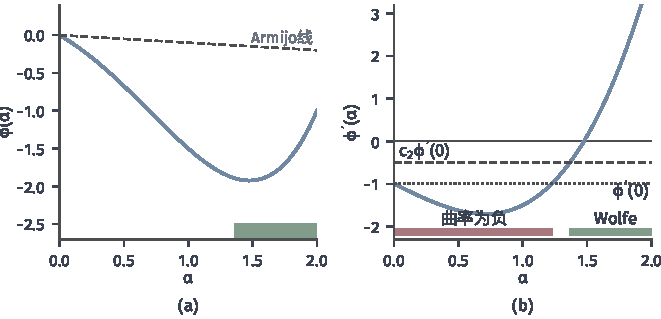
\includegraphics[width=112mm]{figures/05-optimization/02-smooth-optimization/matplotlib/qn-wolfe-curvature/figure.pdf}
  \caption{Wolfe条件怎样保证曲率条件，$\phi'(\alpha)=-1-1.5\alpha+\alpha^3$，$c_1=0.1$，$c_2=0.5$。(a)$\phi$（蓝）和充分下降的边界线（虚线），底部绿条是Wolfe条件的可接受步长。(b)$\phi'$（蓝）。红条上的步长满足$\phi'(\alpha)<\phi'(0)$，曲率条件失败；绿条上的步长满足$\phi'(\alpha)\geq c_2\phi'(0)$。}
  \label{fig:qn-wolfe-curvature}
\end{BookInlineFigure}

\paragraph{不用Wolfe时：跳过与阻尼}
有时线搜索只做回溯，或者步长由别的机制决定，曲率条件就可能不成立。这时有两种处理。

\textbf{跳过更新}：取小的正数$\varepsilon_{\mathrm{c}}$（如$10^{-8}$），当
\begin{equation}
 \langle\bm{s},\bm{y}\rangle\leq\varepsilon_{\mathrm{c}}\lVert\bm{s}\rVert_2\lVert\bm{y}\rVert_2
 \label{eq:qn-skip-rule}
\end{equation}
时令$\bm{W}^{+}=\bm{W}$。它保持正定，代价是这一次测量被扔掉。

\textbf{阻尼更新}：不扔掉测量，而是把$\bm{y}$与$\bm{B}\bm{s}$混合，使混合后的向量满足曲率要求。记曲率比
\[
 \tau=\frac{\langle\bm{s},\bm{y}\rangle}{\bm{s}^\top\bm{B}\bm{s}},
\]
再取
\begin{equation}
 \theta=\begin{cases}1,&\tau\geq0.2,\\\dfrac{0.8}{1-\tau},&\tau<0.2,\end{cases}\qquad
 \bm{r}=\theta\bm{y}+(1-\theta)\bm{B}\bm{s},
 \label{eq:qn-damping}
\end{equation}
再用$\bm{r}$代替$\bm{y}$代入式~\eqref{eq:qn-bfgs-direct}。

这样处理后$\tau<0.2$时的曲率比正好是$0.2$，因为
\[
 \frac{\langle\bm{s},\bm{r}\rangle}{\bm{s}^\top\bm{B}\bm{s}}=\theta\tau+1-\theta=1-\theta(1-\tau)=0.2.
\]
曲率比大于零，由定理~\ref{thm:qn-positive-definite}，$\bm{B}^{+}$正定。

用第~\ref{sec:qn-secant}节的不定例子算一次。取$\bm{B}=\bm{I}$，$\bm{s}=(1,2)^\top$，$\bm{y}=(2,-2)^\top$，则$\bm{s}^\top\bm{B}\bm{s}=5$，$\tau=-0.4$，于是
\[
 \theta=\frac{0.8}{1.4}=\frac47,\qquad
 \bm{r}=\frac47(2,-2)^\top+\frac37(1,2)^\top=\Bigl(\frac{11}{7},-\frac27\Bigr)^\top.
\]
验算：$\langle\bm{s},\bm{r}\rangle=11/7-4/7=1=0.2\times5$。图~\ref{fig:qn-damping}是$\theta$和修正前后曲率比的变化。

要注意阻尼放弃了什么：新矩阵满足$\bm{B}^{+}\bm{s}=\bm{r}$，而不再满足原来的割线条件。下表比较这三种机制。

\begin{BookInlineTable}
  \centering
  \begin{tabular}{lll}
    \toprule
    机制 & 曲率条件 & 代价\\
    \midrule
    Wolfe线搜索 & 由线搜索保证 & 可能多几次函数和梯度计算\\
    跳过更新 & 不成立时不更新 & 丢掉这次测量\\
    阻尼更新 & 由混合后的$\bm{r}$保证 & 放弃原来的割线条件\\
    \bottomrule
  \end{tabular}
  \caption{保持正定性的三种机制。}
  \label{tab:qn-curvature-mechanisms}
\end{BookInlineTable}

\begin{BookInlineFigure}
  \centering
  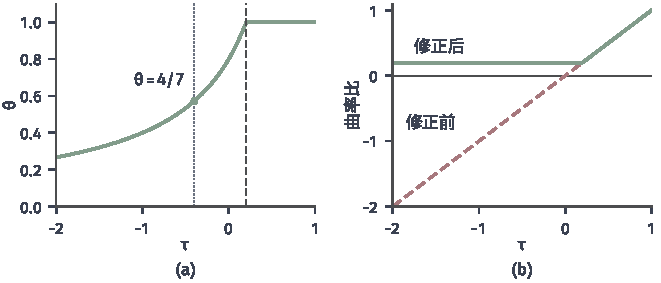
\includegraphics[width=112mm]{figures/05-optimization/02-smooth-optimization/matplotlib/qn-damping/figure.pdf}
  \caption{阻尼更新。(a)式~\eqref{eq:qn-damping}中的混合系数$\theta$随曲率比$\tau$的变化，虚线是阈值$\tau=0.2$，绿点是例中的$\tau=-0.4$，$\theta=4/7$。(b)修正前（红虚线）与修正后（绿）的曲率比，修正后不低于$0.2$。}
  \label{fig:qn-damping}
\end{BookInlineFigure}

\paragraph{计算过程}
下面用贯穿例~\eqref{eq:qn-running-example}完整走一遍BFGS，步长取精确线搜索，它在二次目标上满足Wolfe条件。

\needspace{6\baselineskip}
\paragraph{变量}
\begin{itemize}
 \item $\bm{x}^{(t)}\in\mathbb{R}^{n}$：当前迭代点；$\bm{g}^{(t)}\in\mathbb{R}^{n}$：当前梯度。
 \item $\bm{W}^{(t)}\in\mathbb{R}^{n\times n}$：对称正定的逆曲率近似。
 \item $\bm{d}^{(t)}$、$\alpha^{(t)}$：方向与步长。
 \item $\bm{s}^{(t)}$、$\bm{y}^{(t)}\in\mathbb{R}^{n}$、$\rho^{(t)}$：位移、梯度差与$1/\langle\bm{s}^{(t)},\bm{y}^{(t)}\rangle$。
\end{itemize}

\paragraph{初始化}
选起点$\bm{x}^{(0)}$和对称正定的$\bm{W}^{(0)}$，通常取单位矩阵的倍数，并计算$\bm{g}^{(0)}$。例中初始数据是
\[
 \bm{x}^{(0)}=(4,1)^\top,\qquad\bm{W}^{(0)}=\bm{I},\qquad\bm{g}^{(0)}=(8,8)^\top.
\]

\paragraph{每轮更新}
对$t=0,1,\ldots$依次执行下面的步骤，当$\lVert\bm{g}^{(t)}\rVert_2\leq\varepsilon$时停止。

\begin{enumerate}
\item 由式~\eqref{eq:qn-direction}计算方向$\bm{d}^{(t)}=-\bm{W}^{(t)}\bm{g}^{(t)}$。例中第一轮$\bm{d}^{(0)}=(-8,-8)^\top$。

\item 沿$\bm{d}^{(t)}$做满足式~\eqref{eq:qn-wolfe}的线搜索，优先试$\alpha=1$。例中用精确线搜索，第一轮的步长是
\[
 \alpha^{(0)}=\frac15.
\]

\item 更新迭代点并计算新梯度。例中第一轮得到
\[
 \bm{x}^{(1)}=(2.4,-0.6)^\top,\qquad\bm{g}^{(1)}=(4.8,-4.8)^\top.
\]

\item 由式~\eqref{eq:qn-s-y}计算$\bm{s}^{(t)}$、$\bm{y}^{(t)}$和$\rho^{(t)}$，并检查曲率条件。例中第一轮的$\bm{s}^{(0)}$、$\bm{y}^{(0)}$由式~\eqref{eq:qn-running-pair}给出，且
\[
 \langle\bm{s}^{(0)},\bm{y}^{(0)}\rangle=25.6,\qquad\rho^{(0)}=\frac{1}{25.6}.
\]

\item 用$\bm{s}^{(t)}$、$\bm{y}^{(t)}$、$\rho^{(t)}$构成定理~\ref{thm:qn-bfgs-inverse}中的$\bm{V}$，由式~\eqref{eq:qn-bfgs-inverse}更新$\bm{W}^{(t+1)}$。例中第一轮的两个中间量是
\[
 \bm{V}=\begin{bmatrix}0.8&-0.2\\-0.8&0.2\end{bmatrix},\qquad
 \rho^{(0)}\bm{s}^{(0)}\bigl(\bm{s}^{(0)}\bigr)^\top=\begin{bmatrix}0.1&0.1\\0.1&0.1\end{bmatrix}.
\]
由此得到
\[
 \bm{W}^{(1)}=\bm{V}^\top\bm{V}+\rho^{(0)}\bm{s}^{(0)}\bigl(\bm{s}^{(0)}\bigr)^\top
 =\begin{bmatrix}1.38&-0.22\\-0.22&0.18\end{bmatrix}.
\]
\end{enumerate}

$\bm{W}^{(1)}$的逆是
\[
 \bm{B}^{(1)}=\begin{bmatrix}0.9&1.1\\1.1&6.9\end{bmatrix},
\]
即族~\eqref{eq:qn-secant-family}中$a=0.9$的成员。验算割线条件，$\bm{W}^{(1)}\bm{y}^{(0)}$算出来确实是$(-1.6,-1.6)^\top$，也就是$\bm{s}^{(0)}$。

第二轮按同样的步骤进行。方向和精确步长是
\[
 \bm{d}^{(1)}=-\bm{W}^{(1)}\bm{g}^{(1)}=(-7.68,1.92)^\top,\qquad\alpha^{(1)}=\frac{46.08}{147.456}=\frac{5}{16}.
\]

于是迭代点到达
\[
 \bm{x}^{(2)}=\bm{x}^{(1)}+\alpha^{(1)}\bm{d}^{(1)}=(0,0)^\top,\qquad\bm{g}^{(2)}=\bm{0}.
\]
梯度为零，迭代结束。

为了看矩阵学到了什么，再做一次更新。这时有
\[
 \bm{s}^{(1)}=(-2.4,0.6)^\top,\qquad\bm{y}^{(1)}=(-4.8,4.8)^\top,\qquad\rho^{(1)}=\frac{1}{14.4}.
\]

由式~\eqref{eq:qn-bfgs-inverse}得到
\[
 \bm{W}^{(2)}=\begin{bmatrix}0.5&0\\0&0.125\end{bmatrix}=\bm{A}^{-1}.
\]
最终得到解$\bm{x}^{(2)}=\bm{0}$，而且两次测量之后逆曲率近似恰好等于真实Hessian的逆。图~\ref{fig:qn-bfgs-path}展示了路径和矩阵的变化。

\begin{BookInlineFigure}
  \centering
  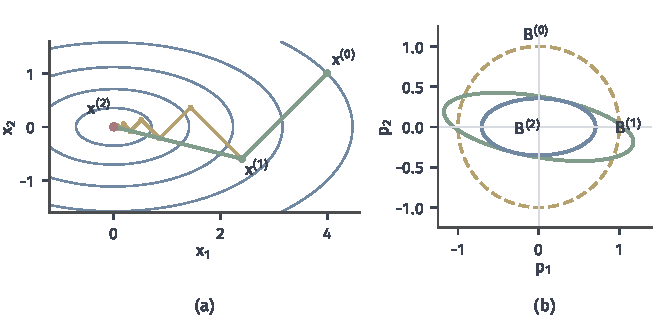
\includegraphics[width=112mm]{figures/05-optimization/02-smooth-optimization/matplotlib/qn-bfgs-path/figure.pdf}
  \caption{贯穿例上的BFGS。(a)蓝线是$f(\bm{x})=x_1^2+4x_2^2$的等高线，绿线是BFGS（$\bm{W}^{(0)}=\bm{I}$，精确线搜索）的两步，黄线是相同起点的最速下降。(b)集合$\{\bm{p}:\bm{p}^\top\bm{B}^{(t)}\bm{p}=1\}$，从圆（黄虚线）经过倾斜的椭圆（绿）变成真实Hessian的等值线（蓝）。}
  \label{fig:qn-bfgs-path}
\end{BookInlineFigure}

这不是巧合。在正定二次目标上使用精确线搜索时，BFGS产生的方向两两关于Hessian共轭，至多$n$步到达最优解，并且$\bm{W}^{(n)}=\bm{A}^{-1}$；第二次更新也没有破坏第一次的测量，例中可以验算$\bm{W}^{(2)}\bm{y}^{(0)}=\bm{s}^{(0)}$。证明用对步数的归纳法，篇幅较长，读者可查阅\scite{math-nocedal2006numerical}。这个结论依赖精确线搜索和二次目标，一般目标上不成立。

\paragraph{DFP与BFGS的对比}
用同一个例子算DFP。第一轮的$\bm{s}^{(0)}$、$\bm{y}^{(0)}$相同，由式~\eqref{eq:qn-dfp-inverse}得到
\[
 \bm{W}^{(1)}_{\mathrm{DFP}}=\frac{1}{170}\begin{bmatrix}177&-23\\-23&27\end{bmatrix}.
\]
它的逆是族~\eqref{eq:qn-secant-family}中$a=1.08$的成员。

矩阵不同，第二轮的方向却平行，$\bm{d}^{(1)}_{\mathrm{DFP}}$约为$(-5.647,1.412)^\top$，正好是BFGS方向的$0.735$倍。原因在于精确线搜索使$\langle\bm{g}^{(1)},\bm{s}^{(0)}\rangle=0$，再由割线条件和$\bm{d}^{(1)}=-\bm{W}^{(1)}\bm{g}^{(1)}$，得到
\[
 \langle\bm{y}^{(0)},\bm{d}^{(1)}\rangle=-\langle\bm{W}^{(1)}\bm{y}^{(0)},\bm{g}^{(1)}\rangle=-\langle\bm{s}^{(0)},\bm{g}^{(1)}\rangle=0.
\]
二维时这确定了方向。两种方法在这个例子上走过完全相同的点。

一旦线搜索不精确，差别就显现出来。图~\ref{fig:qn-dfp-bfgs-scaling}在一个$10$维强凸目标上比较两者，线搜索都满足强Wolfe条件。初始矩阵取$\bm{I}$时，两者都在约$20$步内收敛。

把初始矩阵缩小为$10^{-3}\bm{I}$，相当于矩阵$\bm{B}^{(0)}$的曲率估计过大，BFGS用$74$步恢复，DFP在$300$步后梯度大小仍约为$3.9$。这种从错误的曲率估计中恢复的能力称为自校正。第~\ref{sec:qn-convergence}节会用一个势函数解释BFGS的自校正，那个论证对DFP不适用。这就是实践中通常用BFGS而不用DFP的原因。

\begin{BookInlineFigure}
  \centering
  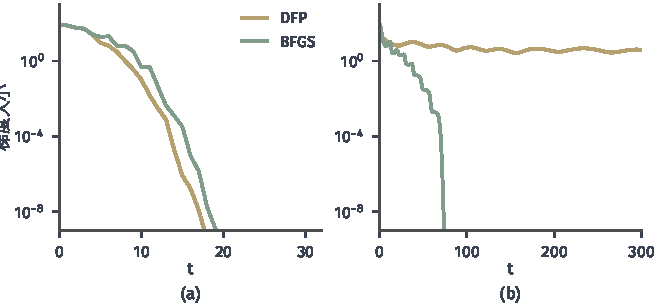
\includegraphics[width=112mm]{figures/05-optimization/02-smooth-optimization/matplotlib/qn-dfp-bfgs-scaling/figure.pdf}
  \caption{BFGS（绿）与DFP（黄）的梯度大小随迭代的变化。目标是$10$维强凸函数$\sum_i(\tfrac12c_iz_i^2+\ln\cosh z_i)$，其中$\bm{z}=\bm{Q}\bm{x}$，$\bm{Q}$是固定的正交矩阵，$c_i$在$[0.1,100]$上对数等距；线搜索为强Wolfe条件，$c_1=10^{-4}$，$c_2=0.9$。(a)$\bm{W}^{(0)}=\bm{I}$。(b)$\bm{W}^{(0)}=10^{-3}\bm{I}$，注意横轴范围不同。}
  \label{fig:qn-dfp-bfgs-scaling}
\end{BookInlineFigure}

\section{SR1}
\label{sec:qn-sr1}

BFGS为了保持正定，把负曲率的测量拒之门外。可是目标在某些方向确实向下弯时，这恰恰是有用的信息。这就需要回答：只用一个秩一项能否满足割线条件，这样得到的矩阵有什么长处，又有什么风险？

\paragraph{主要思想：只有一种秩一修正}
设$\bm{B}^{+}=\bm{B}+\sigma\bm{v}\bm{v}^\top$，其中$\sigma=\pm1$。记割线残差$\bm{r}=\bm{y}-\bm{B}\bm{s}$，把割线条件写成
\[
 \sigma\langle\bm{v},\bm{s}\rangle\bm{v}=\bm{r}.
\]
左边是$\bm{v}$的数乘，所以$\bm{v}$必须平行于$\bm{r}$。把$\bm{v}$取成$\bm{r}$的倍数后，$\sigma$和倍数只有一种可能，由此得到\term{对称秩一更新}（symmetric rank-one update，SR1）：
\begin{equation}
 \bm{B}^{+}=\bm{B}+\frac{\bm{r}\bm{r}^\top}{\langle\bm{r},\bm{s}\rangle},\qquad\bm{r}=\bm{y}-\bm{B}\bm{s}.
 \label{eq:qn-sr1-direct}
\end{equation}

与第~\ref{sec:qn-dfp-bfgs}节不同，这里的更新由割线条件和“秩一”完全确定，没有选择余地。验算割线条件：$\bm{B}^{+}\bm{s}=\bm{B}\bm{s}+\bm{r}=\bm{y}$。

把同样的推导用在逆矩阵上，并记$\bm{w}=\bm{s}-\bm{W}\bm{y}$，得到
\begin{equation}
 \bm{W}^{+}=\bm{W}+\frac{\bm{w}\bm{w}^\top}{\langle\bm{w},\bm{y}\rangle}.
 \label{eq:qn-sr1-inverse}
\end{equation}
只要$\bm{B}$、$\bm{B}^{+}$都可逆，式~\eqref{eq:qn-sr1-inverse}的$\bm{W}^{+}$就是式~\eqref{eq:qn-sr1-direct}的$\bm{B}^{+}$的逆，这可以用Sherman--Morrison公式验证。SR1自己是自己的对偶，所以不像BFGS和DFP那样分成两种方法。

\paragraph{计算过程}
SR1不需要线搜索来保持什么性质，下面就用单位步长演示它。仍用贯穿例，这一次不做线搜索，每步直接走完整的$-\bm{W}^{(t)}\bm{g}^{(t)}$。

\needspace{6\baselineskip}
\paragraph{变量}
\begin{itemize}
 \item $\bm{x}^{(t)}$、$\bm{g}^{(t)}\in\mathbb{R}^{n}$：当前点与梯度。
 \item $\bm{W}^{(t)}\in\mathbb{R}^{n\times n}$：对称的逆曲率近似，不要求正定。
 \item $\bm{s}^{(t)}$、$\bm{y}^{(t)}$：位移与梯度差；$\bm{w}^{(t)}$：式~\eqref{eq:qn-sr1-inverse}中逆形式的割线残差。
 \item $c_{\mathrm{r}}>0$：判断分母是否过小的阈值。
\end{itemize}

\paragraph{初始化}
选起点和对称的$\bm{W}^{(0)}$。例中初始数据是
\[
 \bm{x}^{(0)}=(4,1)^\top,\qquad\bm{W}^{(0)}=\bm{I},\qquad\bm{g}^{(0)}=(8,8)^\top.
\]

\paragraph{每轮更新}
对$t=0,1,\ldots$依次执行下面的步骤，当$\lVert\bm{g}^{(t)}\rVert_2\leq\varepsilon$时停止。

\begin{enumerate}
\item 计算$\bm{s}^{(t)}=-\bm{W}^{(t)}\bm{g}^{(t)}$，令$\bm{x}^{(t+1)}=\bm{x}^{(t)}+\bm{s}^{(t)}$，并读取$\bm{g}^{(t+1)}$。例中第一轮得到
\[
 \bm{s}^{(0)}=(-8,-8)^\top,\qquad\bm{x}^{(1)}=(-4,-7)^\top,\qquad\bm{g}^{(1)}=(-8,-56)^\top.
\]
目标值从$20$升到了$212$，这一步在目标上是失败的，但测量仍然有用。

\item 计算$\bm{y}^{(t)}=\bm{g}^{(t+1)}-\bm{g}^{(t)}$和$\bm{w}^{(t)}$。例中第一轮得到
\[
 \bm{y}^{(0)}=(-16,-64)^\top,\qquad\bm{w}^{(0)}=(8,56)^\top,\qquad\langle\bm{w}^{(0)},\bm{y}^{(0)}\rangle=-3712.
\]

\item 若$\langle\bm{w}^{(t)},\bm{y}^{(t)}\rangle$的绝对值不小于$c_{\mathrm{r}}\lVert\bm{w}^{(t)}\rVert_2\lVert\bm{y}^{(t)}\rVert_2$，由式~\eqref{eq:qn-sr1-inverse}更新$\bm{W}^{(t+1)}$；否则令$\bm{W}^{(t+1)}=\bm{W}^{(t)}$。例中第一轮分母足够大，更新后得到
\[
 \bm{W}^{(1)}=\frac{1}{58}\begin{bmatrix}57&-7\\-7&9\end{bmatrix}.
\]
\end{enumerate}

第二轮的位移与新点是
\[
 \bm{s}^{(1)}=\frac{1}{29}(32,224)^\top,\qquad\bm{x}^{(2)}=\frac{1}{29}(-84,21)^\top\approx(-2.897,0.724)^\top.
\]

梯度差和逆形式残差是
\[
 \bm{y}^{(1)}=\frac{1}{29}(64,1792)^\top,\qquad\bm{w}^{(1)}=\frac{1344}{841}(4,-1)^\top.
\]

分母约为$-84.64$，更新量是$-\tfrac{7}{232}$乘以$\begin{bmatrix}16&-4\\-4&1\end{bmatrix}$，于是
\[
 \bm{W}^{(2)}=\begin{bmatrix}0.5&0\\0&0.125\end{bmatrix}=\bm{A}^{-1}.
\]

第三轮的方向已经是Newton方向，一步到达解：
\[
 \bm{s}^{(2)}=\frac{1}{29}(84,-21)^\top,\qquad\bm{x}^{(3)}=\bm{0},\qquad\bm{g}^{(3)}=\bm{0}.
\]
迭代结束，最终得到解$\bm{x}^{(3)}=\bm{0}$，用了$n+1=3$步。图~\ref{fig:qn-sr1-path}是这条路径。

\begin{BookInlineFigure}
  \centering
  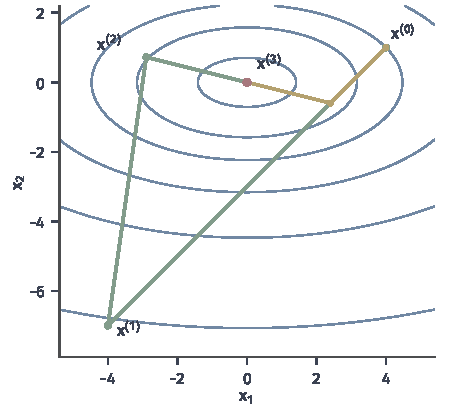
\includegraphics[width=78mm]{figures/05-optimization/02-smooth-optimization/matplotlib/qn-sr1-path/figure.pdf}
  \caption{贯穿例上的SR1路径（绿）：$\bm{W}^{(0)}=\bm{I}$，每步取单位步长。第一步远远越过谷底，目标值从$20$升到$212$，但两次测量足以确定$\bm{A}$，第三步准确落在最优解（红）。黄线是精确线搜索的BFGS路径，用作对照。}
  \label{fig:qn-sr1-path}
\end{BookInlineFigure}

\paragraph{有限步终止}
这个现象对二次目标普遍成立，而且完全不依赖步长的选取。下面的定理把BFGS那里“两次测量都不丢失”的现象，以更强的形式写了下来。

\begin{theorem}[SR1的遗传性质]
\label{thm:qn-sr1-hereditary}
设$f$是二次函数，Hessian为对称矩阵$\bm{A}$，于是$\bm{y}^{(j)}=\bm{A}\bm{s}^{(j)}$。设$\bm{B}^{(j+1)}$由SR1按式~\eqref{eq:qn-sr1-direct}逐次得到，所有分母非零。则对每个$k$，
\begin{equation}
 \bm{B}^{(k)}\bm{s}^{(j)}=\bm{y}^{(j)},\qquad j=0,1,\ldots,k-1.
 \label{eq:qn-sr1-hereditary}
\end{equation}
特别地，若$\bm{s}^{(0)},\ldots,\bm{s}^{(n-1)}$线性无关，则$\bm{B}^{(n)}=\bm{A}$。
\end{theorem}

\begin{proof}
对$k$归纳。$k=1$时就是割线条件。设式~\eqref{eq:qn-sr1-hereditary}对$k$成立，并记$\bm{r}=\bm{y}^{(k)}-\bm{B}^{(k)}\bm{s}^{(k)}$。

对$j<k$，由归纳假设、对称性和$\bm{y}^{(j)}=\bm{A}\bm{s}^{(j)}$，得到
\[
 \begin{aligned}
 \langle\bm{r},\bm{s}^{(j)}\rangle
 &=\langle\bm{y}^{(k)},\bm{s}^{(j)}\rangle-\langle\bm{s}^{(k)},\bm{B}^{(k)}\bm{s}^{(j)}\rangle\\
 &=\langle\bm{A}\bm{s}^{(k)},\bm{s}^{(j)}\rangle-\langle\bm{s}^{(k)},\bm{A}\bm{s}^{(j)}\rangle=0.
 \end{aligned}
\]

所以秩一修正项作用在旧位移上为零：
\[
 \bm{B}^{(k+1)}\bm{s}^{(j)}=\bm{B}^{(k)}\bm{s}^{(j)}+\bm{r}\,\frac{\langle\bm{r},\bm{s}^{(j)}\rangle}{\langle\bm{r},\bm{s}^{(k)}\rangle}=\bm{y}^{(j)}.
\]
$j=k$时是割线条件本身，归纳完成。

$\bm{s}^{(j)}$线性无关时，把它们排成可逆矩阵$\bm{S}$，式~\eqref{eq:qn-sr1-hereditary}说明$\bm{B}^{(n)}\bm{S}=\bm{A}\bm{S}$，右乘$\bm{S}^{-1}$即得。
\end{proof}

所以$\bm{A}$可逆、$\bm{B}^{(n)}$之前的各步线性无关时，单位步长的SR1至多$n+1$步到达驻点。定理没有要求$\bm{A}$正定，也没有要求线搜索，这是SR1与BFGS的重要区别。

\paragraph{分母可能为零}
SR1的麻烦全在分母$\langle\bm{r},\bm{s}\rangle$上。若$\bm{r}\neq\bm{0}$而$\langle\bm{r},\bm{s}\rangle=0$，则根本不存在满足割线条件的对称秩一修正。原因是由$\sigma\langle\bm{v},\bm{s}\rangle\bm{v}=\bm{r}$与$\bm{s}$作内积，得到
\[
 \sigma\langle\bm{v},\bm{s}\rangle^2=\langle\bm{r},\bm{s}\rangle=0.
\]
于是$\langle\bm{v},\bm{s}\rangle=0$，等式左边就是零向量，与$\bm{r}\neq\bm{0}$矛盾。

这种情况确实会出现。取$\bm{A}=\operatorname{diag}(2,8)$，$\bm{B}=\operatorname{diag}(3,7)$，$\bm{s}=(1,1)^\top$，则
\[
 \bm{y}=(2,8)^\top,\qquad\bm{r}=(-1,1)^\top,\qquad\langle\bm{r},\bm{s}\rangle=0.
\]

分母接近零同样有害。把$\bm{s}$换成$(1,1+\epsilon)^\top$，分母是$2\epsilon+\epsilon^2$，而$\lVert\bm{r}\rVert_2$约为$\sqrt2$，修正量的Frobenius范数约为$1/\epsilon$。图~\ref{fig:qn-sr1-denominator}展示了这种放大：$\epsilon=10^{-4}$时修正量约为$10^{4}$，矩阵几乎被这一次修正淹没。

\begin{BookInlineFigure}
  \centering
  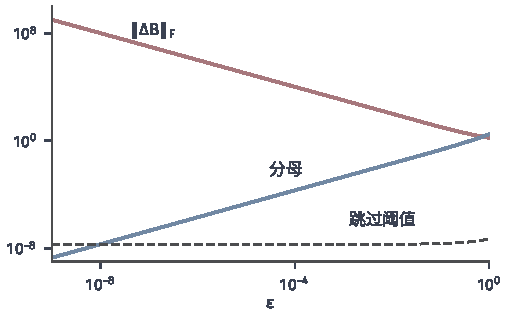
\includegraphics[width=86mm]{figures/05-optimization/02-smooth-optimization/matplotlib/qn-sr1-denominator/figure.pdf}
  \caption{SR1的分母接近零时的放大效应：$\bm{A}=\operatorname{diag}(2,8)$，$\bm{B}=\operatorname{diag}(3,7)$，$\bm{s}=(1,1+\epsilon)^\top$。蓝线是分母$\lvert\langle\bm{r},\bm{s}\rangle\rvert$，红线是修正量$\lVert\Delta\bm{B}\rVert_F$；虚线是取$c_{\mathrm{r}}=10^{-8}$时的跳过阈值$c_{\mathrm{r}}\lVert\bm{r}\rVert_2\lVert\bm{s}\rVert_2$，分母低于它就不更新。}
  \label{fig:qn-sr1-denominator}
\end{BookInlineFigure}

所以SR1配有跳过规则，这就是计算过程第三步的判断，直接形式下写成
\begin{equation}
 \lvert\langle\bm{r},\bm{s}\rangle\rvert\geq c_{\mathrm{r}}\lVert\bm{r}\rVert_2\lVert\bm{s}\rVert_2,
 \label{eq:qn-sr1-safeguard}
\end{equation}
通常取$c_{\mathrm{r}}=10^{-8}$。不满足时保持$\bm{B}^{+}=\bm{B}$。

式~\eqref{eq:qn-sr1-safeguard}中的角度形式比绝对阈值合理：它问的是$\bm{r}$与$\bm{s}$是否几乎垂直，与两个向量的长度无关。跳过很少发生，因为分母近零需要$\bm{r}$恰好几乎垂直于$\bm{s}$。

\paragraph{SR1通常不保持正定}
BFGS的更新中，分母$\langle\bm{s},\bm{y}\rangle$与修正项的符号都受控制。SR1的分母可正可负，修正项的符号跟着变，所以正定矩阵可能变成不定矩阵，即使目标强凸。

取贯穿例的目标，$\bm{x}^{(0)}=(-4,-0.5)^\top$，$\bm{B}^{(0)}=4\bm{I}$，单位步长。这时
\[
 \bm{g}^{(0)}=(-8,-4)^\top,\qquad\bm{s}^{(0)}=(2,1)^\top,\qquad\bm{y}^{(0)}=(4,8)^\top.
\]

$\bm{B}^{(0)}\bm{s}^{(0)}=(8,4)^\top$，所以残差和分母是
\[
 \bm{r}=(-4,4)^\top,\qquad\langle\bm{r},\bm{s}^{(0)}\rangle=-4.
\]
代入式~\eqref{eq:qn-sr1-direct}，得到
\[
 \bm{B}^{(1)}=\begin{bmatrix}0&4\\4&0\end{bmatrix}.
\]
它的特征值是$\pm4$，不定。验算割线条件：$\bm{B}^{(1)}\bm{s}^{(0)}=(4,8)^\top=\bm{y}^{(0)}$。

新点是$\bm{x}^{(1)}=(-2,0.5)^\top$，梯度$\bm{g}^{(1)}=(-4,4)^\top$。若仍然用公式~\eqref{eq:qn-direction}算方向，得到
\[
 \bm{d}=-\bigl(\bm{B}^{(1)}\bigr)^{-1}\bm{g}^{(1)}=(-1,1)^\top,\qquad\langle\bm{g}^{(1)},\bm{d}\rangle=8>0.
\]

这是一个上升方向。$\bm{d}$是模型的驻点，但模型不定，驻点是鞍点而不是极小点。沿它走一步，目标从$5$升到$18$。第~\ref{sec:qn-secant}节的下降论证依赖$\bm{W}$正定，这里前提已经不成立，所以不能把BFGS方向的下降分析搬过来。

\paragraph{不定模型与信赖域}
不定的$\bm{B}$并非无用，用错的只是“跑到模型驻点”这个做法。模型$m(\bm{p})$在$\bm{p}$的某些方向向下弯，这时它没有极小点，但在一个有界的范围内它有。第~\ref{chap:trust-region}章的信赖域方法正是如此：只在以当前点为中心、半径为$\Delta$的球内最小化模型，并用实际下降检验这个候选步。

继续上面的例子，取$\Delta=1$。$\bm{B}^{(1)}$的负特征值$-4$对应单位特征向量$\bm{v}=(1,-1)^\top/\sqrt2$，而$\bm{g}^{(1)}=-4\sqrt2\,\bm{v}$恰好全部落在这个方向上。沿$\bm{p}=\beta\bm{v}$，模型的变化量是
\[
 m(\beta\bm{v})-m(\bm{0})=-4\sqrt2\,\beta-2\beta^2.
\]

在$\lvert\beta\rvert\leq1$上它在$\beta=1$处最小，所以候选步是
\[
 \bm{p}_{\Delta}=\frac{1}{\sqrt2}(1,-1)^\top.
\]
它是下降方向，因为与梯度的内积是$-4\sqrt2<0$。沿它走一步，目标从$5$降到约$1.843$。图~\ref{fig:qn-sr1-saddle}比较了两个候选步。

\begin{BookInlineFigure}
  \centering
  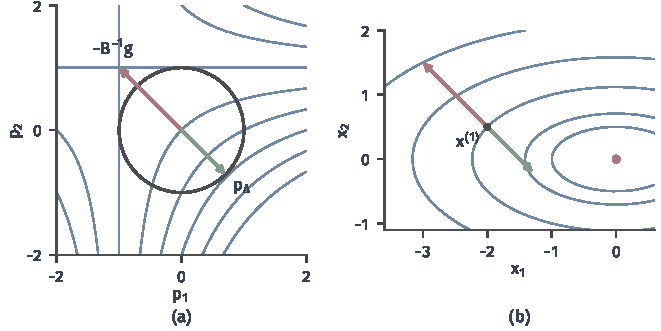
\includegraphics[width=112mm]{figures/05-optimization/02-smooth-optimization/matplotlib/qn-sr1-saddle/figure.pdf}
  \caption{不定模型下的两个候选步，$\bm{B}=\begin{bmatrix}0&4\\4&0\end{bmatrix}$，$\bm{g}=(-4,4)^\top$，圆的半径为$1$。(a)蓝线是模型$m(\bm{p})$的等值线，呈鞍形。红箭头是模型的驻点$-\bm{B}^{-1}\bm{g}$，绿箭头是圆内模型的极小点。(b)同样的两步放到真实目标$x_1^2+4x_2^2$的等高线上，红步使目标上升，绿步使目标下降。}
  \label{fig:qn-sr1-saddle}
\end{BookInlineFigure}

这也解释了SR1和BFGS的分工。BFGS的矩阵总是正定的，方向一定下降，配线搜索很自然；但它看不到负曲率，也只有测量满足曲率条件才能更新。SR1能记录负曲率，在二次目标上对步长没有要求，但需要有界的模型来消化不定性。

\begin{BookInlineTable}
  \centering
  \begin{tabular}{lll}
    \toprule
    比较项 & BFGS & SR1\\
    \midrule
    修正的秩 & 二 & 一\\
    更新的前提 & 曲率条件 & 分母不过小\\
    正定性 & 保持 & 通常不保持\\
    负曲率信息 & 不能表示 & 可以表示\\
    配套的全局化手段 & Wolfe线搜索 & 信赖域\\
    \bottomrule
  \end{tabular}
  \caption{BFGS与SR1的对比。}
  \label{tab:qn-bfgs-sr1}
\end{BookInlineTable}

\section{L-BFGS}
\label{sec:qn-lbfgs}

BFGS不必解方程，但仍要保存一个$n\times n$的稠密矩阵。$n=10^6$时这需要约$10^{12}$个元素的存储，通常根本放不下。不保存矩阵，能否仍然算出$\bm{W}^{(t)}\bm{g}^{(t)}$？

\paragraph{主要思想：只保留最近的测量}
BFGS的$\bm{W}^{(t)}$完全由$\bm{W}^{(0)}$和所有的$(\bm{s}^{(j)},\bm{y}^{(j)})$决定。旧测量在非二次目标上已经过时，于是\term{有限记忆BFGS}（limited-memory BFGS，L-BFGS）只保留最近$r$对，$r$称为记忆长度，常取$3$到$30$。

存储从约$n^2/2$个数降到$2rn$个数。每一轮都重新从一个简单的初始矩阵$\gamma^{(t)}\bm{I}$出发，把这$r$对依次用式~\eqref{eq:qn-bfgs-inverse}更新一遍，得到的矩阵就是这一轮的$\bm{W}^{(t)}$。

记下面$r$次更新的中间矩阵为$\bm{W}_{[j]}$，下标$j$从$t-r$走到$t$。起点和递推是
\begin{equation}
 \bm{W}_{[t-r]}=\gamma^{(t)}\bm{I},\qquad
 \bm{W}_{[j+1]}=\bigl(\bm{V}^{(j)}\bigr)^\top\bm{W}_{[j]}\bm{V}^{(j)}+\rho^{(j)}\bm{s}^{(j)}\bigl(\bm{s}^{(j)}\bigr)^\top,
 \label{eq:qn-lbfgs-recursion}
\end{equation}
其中$\bm{V}^{(j)}$由第$j$对向量按定理~\ref{thm:qn-bfgs-inverse}的方式构成，最后$\bm{W}^{(t)}=\bm{W}_{[t]}$。显式写出这些矩阵要$O(n^2)$的存储，我们其实只需要它乘一个向量的结果。

\paragraph{主要思想：两层递推}
令$\bm{q}_{[t]}=\bm{g}^{(t)}$，想算$\bm{W}_{[t]}\bm{q}_{[t]}$。把递推~\eqref{eq:qn-lbfgs-recursion}作用在向量$\bm{q}_{[j+1]}$上，先算出向右侧的两个量：
\[
 \xi^{(j)}=\rho^{(j)}\langle\bm{s}^{(j)},\bm{q}_{[j+1]}\rangle,\qquad
 \bm{q}_{[j]}=\bm{V}^{(j)}\bm{q}_{[j+1]}=\bm{q}_{[j+1]}-\xi^{(j)}\bm{y}^{(j)}.
\]

于是一次更新对向量的作用可以写成
\[
 \bm{W}_{[j+1]}\bm{q}_{[j+1]}=\bigl(\bm{V}^{(j)}\bigr)^\top\bm{W}_{[j]}\bm{q}_{[j]}+\xi^{(j)}\bm{s}^{(j)}.
\]
右端的$\bm{W}_{[j]}\bm{q}_{[j]}$是同样形式、但下标小一的问题。所以计算分两层：第一层让$j$从$t-1$递减到$t-r$，把$\bm{q}$一路算下去，记下所有$\xi^{(j)}$。

第一层走到底时，最内层的矩阵是$\gamma^{(t)}\bm{I}$，令$\bm{z}_{[t-r]}=\gamma^{(t)}\bm{q}_{[t-r]}$。记$\bm{z}_{[j]}=\bm{W}_{[j]}\bm{q}_{[j]}$，把$\bm{V}^{(j)}$的转置展开，得到第二层的递推：
\begin{equation}
 \eta^{(j)}=\rho^{(j)}\langle\bm{y}^{(j)},\bm{z}_{[j]}\rangle,\qquad
 \bm{z}_{[j+1]}=\bm{z}_{[j]}+\bigl(\xi^{(j)}-\eta^{(j)}\bigr)\bm{s}^{(j)}.
 \label{eq:qn-lbfgs-second-loop}
\end{equation}
第二层让$j$从$t-r$递增到$t-1$，最后的$\bm{z}_{[t]}$就是$\bm{W}^{(t)}\bm{g}^{(t)}$。这就是\term{双循环递推}（two-loop recursion），图~\ref{fig:qn-lbfgs-two-loop}是它的结构。

\begin{BookInlineFigure}
  \centering
  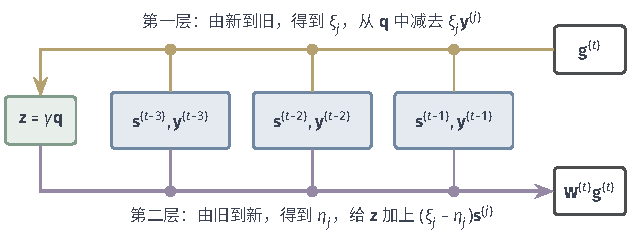
\includegraphics[width=106mm]{figures/05-optimization/02-smooth-optimization/tikz/qn-lbfgs-two-loop/figure.pdf}
  \caption{L-BFGS的双循环递推，$r=3$。蓝框是保存的三对向量。第一层（黄）从梯度出发，由最新一对走到最旧一对；中间乘初始矩阵$\gamma\bm{I}$（绿框）；第二层（紫）由最旧一对走回最新一对，输出$\bm{W}^{(t)}\bm{g}^{(t)}$。全程只有向量内积和向量加法。}
  \label{fig:qn-lbfgs-two-loop}
\end{BookInlineFigure}

每一层对每对向量做一次内积和一次向量加法，再加上中间的缩放，每个方向的运算量约为$(4r+1)n$次乘法。矩阵本身从未出现。

\paragraph{主要思想：初始缩放}
最内层的矩阵决定了双循环不了解的那些方向上的尺度。L-BFGS一般取
\begin{equation}
 \gamma^{(t)}=\frac{\langle\bm{s}^{(t-1)},\bm{y}^{(t-1)}\rangle}{\langle\bm{y}^{(t-1)},\bm{y}^{(t-1)}\rangle}.
 \label{eq:qn-lbfgs-gamma}
\end{equation}

它的含义可以由式~\eqref{eq:qn-average-hessian}看出。设平均Hessian正定，并把$(\bar{\bm{H}}^{(t-1)})^{1/2}\bm{s}^{(t-1)}$记作$\bm{z}$，则
\[
 \frac{1}{\gamma^{(t)}}=\frac{\bm{z}^\top\bar{\bm{H}}^{(t-1)}\bm{z}}{\bm{z}^\top\bm{z}}.
\]
所以$1/\gamma^{(t)}$是平均Hessian的一个Rayleigh商，落在其最小与最大特征值之间，是目标曲率的一个合理的标量估计。

\paragraph{主要思想：曲率检查}
与完整BFGS一样，存入的$(\bm{s}^{(j)},\bm{y}^{(j)})$必须满足$\langle\bm{s}^{(j)},\bm{y}^{(j)}\rangle>0$，否则式~\eqref{eq:qn-lbfgs-recursion}不再保证正定，算出的方向可能不下降。Wolfe线搜索使这一点自动成立。只用回溯时，要加上跳过规则：满足式~\eqref{eq:qn-skip-rule}的这一对不存入，窗口保持原样。

\paragraph{计算过程}
下面用贯穿例演示$r=2$的L-BFGS。为了不让第一层的系数因为正交性而消失，第一步取$\alpha^{(0)}=1/8$而不是精确步长，以后都用单位步长；这些步长都满足$c_1=10^{-4}$、$c_2=0.9$的Wolfe条件。

\needspace{6\baselineskip}
\paragraph{变量}
\begin{itemize}
 \item $\bm{x}^{(t)}$、$\bm{g}^{(t)}\in\mathbb{R}^{n}$：当前点与梯度。
 \item 窗口：最多$r$组$(\bm{s}^{(j)},\bm{y}^{(j)},\rho^{(j)})$，$\bm{s}^{(j)},\bm{y}^{(j)}\in\mathbb{R}^{n}$，$\rho^{(j)}$是标量，从旧到新排列。
 \item 第一层的向量$\bm{q}\in\mathbb{R}^{n}$和系数$\xi^{(j)}$；第二层的向量$\bm{z}\in\mathbb{R}^{n}$和系数$\eta^{(j)}$。
 \item $\gamma^{(t)}>0$：初始矩阵的缩放。
\end{itemize}

\paragraph{初始化}
选起点，窗口置空。窗口为空时取$\gamma^{(0)}=1$，方向就是负梯度。例中第一轮的数据是
\[
 \bm{x}^{(0)}=(4,1)^\top,\qquad\bm{g}^{(0)}=(8,8)^\top,\qquad\bm{d}^{(0)}=(-8,-8)^\top.
\]
取$\alpha^{(0)}=1/8$，走完后有
\[
 \bm{x}^{(1)}=(3,0)^\top,\qquad\bm{g}^{(1)}=(6,0)^\top.
\]
第一对测量及其$\rho$是
\[
 \bm{s}^{(0)}=(-1,-1)^\top,\qquad\bm{y}^{(0)}=(-2,-8)^\top,\qquad\rho^{(0)}=0.1.
\]

\paragraph{每轮更新}
对$t=1,2,\ldots$依次执行下面的步骤，当$\lVert\bm{g}^{(t)}\rVert_2\leq\varepsilon$时停止。

\begin{enumerate}
\item 第一层，令$\bm{q}=\bm{g}^{(t)}$，对窗口中的$j$由新到旧，依次计算
\[
 \xi^{(j)}=\rho^{(j)}\langle\bm{s}^{(j)},\bm{q}\rangle,\qquad\bm{q}\leftarrow\bm{q}-\xi^{(j)}\bm{y}^{(j)}.
\]
例中$t=1$时窗口只有一对，结果是
\[
 \xi^{(0)}=-0.6,\qquad\bm{q}=(4.8,-4.8)^\top.
\]

\item 由式~\eqref{eq:qn-lbfgs-gamma}计算$\gamma^{(t)}$，并令$\bm{z}=\gamma^{(t)}\bm{q}$。例中$t=1$时$\langle\bm{y}^{(0)},\bm{y}^{(0)}\rangle=68$，于是
\[
 \gamma^{(1)}=\frac{10}{68}=\frac{5}{34},\qquad\bm{z}\approx(0.7059,-0.7059)^\top.
\]

\item 第二层，对窗口中的$j$由旧到新，按式~\eqref{eq:qn-lbfgs-second-loop}更新$\bm{z}$。例中$t=1$时得到
\[
 \eta^{(0)}\approx0.4235,\qquad\bm{z}\approx(1.7294,0.3176)^\top.
\]

\item 令$\bm{d}^{(t)}=-\bm{z}$，线搜索后得到新点和新梯度。例中$t=1$时取$\alpha^{(1)}=1$，结果是
\[
 \bm{d}^{(1)}\approx(-1.7294,-0.3176)^\top,\qquad\bm{x}^{(2)}\approx(1.2706,-0.3176)^\top.
\]

\item 计算$\bm{s}^{(t)}$、$\bm{y}^{(t)}$和$\rho^{(t)}$，曲率检查通过后存入窗口；若窗口超过$r$对，丢弃最旧的一对。例中$t=1$时
\[
 \bm{y}^{(1)}\approx(-3.4588,-2.5412)^\top,\qquad\rho^{(1)}\approx0.14730.
\]
窗口现在有两对，还没有超过$r=2$。
\end{enumerate}

$t=2$时窗口有两对，能看到完整的双循环。此时的梯度是
\[
 \bm{g}^{(2)}\approx(2.5412,-2.5412)^\top.
\]
第一层由新到旧的两次计算是
\[
 \begin{aligned}
 j=1:&\quad\xi^{(1)}\approx-0.5284,\quad\bm{q}\approx(0.7134,-3.8840)^\top,\\
 j=0:&\quad\xi^{(0)}\approx0.3171,\quad\bm{q}\approx(1.3475,-1.3475)^\top.
 \end{aligned}
\]

中间的缩放使用最新一对，结果是
\[
 \gamma^{(2)}\approx0.36854,\qquad\bm{z}\approx(0.4966,-0.4966)^\top.
\]

第二层由旧到新的两次计算是
\[
 \begin{aligned}
 j=0:&\quad\eta^{(0)}\approx0.2980,\quad\bm{z}\approx(0.4775,-0.5157)^\top,\\
 j=1:&\quad\eta^{(1)}\approx-0.0503,\quad\bm{z}\approx(1.3045,-0.3638)^\top.
 \end{aligned}
\]

取单位步长，新的点是
\[
 \bm{d}^{(2)}\approx(-1.3045,0.3638)^\top,\qquad\bm{x}^{(3)}\approx(-0.0339,0.0462)^\top.
\]
$t=3$时窗口超过$r=2$，$\bm{s}^{(0)}$、$\bm{y}^{(0)}$被丢弃。后续各轮的结果列在表~\ref{tab:qn-lbfgs-run}中。取$\varepsilon=10^{-3}$，在$t=7$时停止，表中最后一行就是最终得到的点。

\begin{BookInlineTable}
  \centering
  \begin{tabular}{rccc}
    \toprule
    $t$ & $\bm{x}^{(t)}$（近似） & $\lVert\bm{g}^{(t)}\rVert_2$ & $f(\bm{x}^{(t)})$\\
    \midrule
    0 & $(4,\ 1)$ & $11.31$ & $20$\\
    1 & $(3,\ 0)$ & $6$ & $9$\\
    2 & $(1.2706,\ -0.3176)$ & $3.594$ & $2.018$\\
    3 & $(-0.0339,\ 0.0462)$ & $0.3755$ & $9.7\times10^{-3}$\\
    4 & $(-0.0150,\ -0.0134)$ & $0.1115$ & $9.4\times10^{-4}$\\
    5 & $(-0.0012,\ -0.0001)$ & $2.4\times10^{-3}$ & $1.4\times10^{-6}$\\
    6 & $(-0.0004,\ 0.0001)$ & $1.1\times10^{-3}$ & $1.8\times10^{-7}$\\
    7 & $(0.000005,\ -0.000005)$ & $4.1\times10^{-5}$ & $1.2\times10^{-10}$\\
    \bottomrule
  \end{tabular}
  \caption{贯穿例上$r=2$的L-BFGS各轮结果，$\alpha^{(0)}=1/8$，其余各轮$\alpha^{(t)}=1$。}
  \label{tab:qn-lbfgs-run}
\end{BookInlineTable}

和完整BFGS的两步终止比较，这里用了七步，尽管$r$已经等于变量个数$n$。差别来自两处：步长不是精确的，而且每一轮都从$\gamma^{(t)}\bm{I}$重新开始，矩阵不再累积。

窗口尚未被填满时，只有初始矩阵不同；若初始矩阵也取同一个$\gamma\bm{I}$，L-BFGS与完整BFGS算出的方向完全相同。两者的差别从第一次丢弃旧测量开始。

\paragraph{记忆长度的影响}
图~\ref{fig:qn-lbfgs-memory}在一个$200$维、系数跨越六个数量级的强凸目标上比较不同的$r$。迭代数随$r$增大而减少，但下降缓慢：$r$从$1$增加到$100$，迭代数从$429$降到$218$，而方向运算量大约增加$50$倍。

因此$r$的选择取决于梯度和方向计算哪个贵：梯度贵时，多用一点记忆来节省梯度是值得的；梯度便宜时，小的$r$更省。图中的数据只说明这一个目标的情况，不是普遍的定量规律。

\begin{BookInlineFigure}
  \centering
  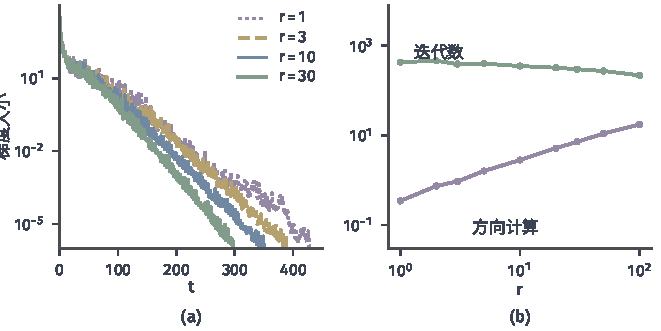
\includegraphics[width=112mm]{figures/05-optimization/02-smooth-optimization/matplotlib/qn-lbfgs-memory/figure.pdf}
  \caption{记忆长度的影响。目标是$200$维的$\sum_i(\tfrac12c_iz_i^2+\ln\cosh z_i)$，$\bm{z}=\bm{Q}\bm{x}$，$\bm{Q}$是固定的正交矩阵，$c_i$在$[10^{-3},10^{3}]$上对数等距，强Wolfe线搜索，$c_2=0.9$。(a)不同$r$下的梯度大小。(b)达到梯度大小$10^{-6}$的迭代数（绿）和这些迭代中方向计算的总乘法次数（紫，单位百万次，按每步$4rn$估算）。}
  \label{fig:qn-lbfgs-memory}
\end{BookInlineFigure}

\paragraph{初始缩放的影响}
图~\ref{fig:qn-lbfgs-scaling}比较有缩放~\eqref{eq:qn-lbfgs-gamma}和始终用$\gamma=1$的两种做法，记忆长度都是$r=10$，目标的曲率整体偏大。

没有缩放时，单位矩阵相对于真实曲率过大，方向过长，线搜索不得不反复收缩，$292$轮迭代共用了$5012$次函数和梯度计算。有缩放时只用$130$轮迭代和$268$次计算。这个对比说明，在大尺度问题上，第~\ref{sec:qn-secant}节“优先试单位步长”的策略依赖矩阵有正确的尺度。

\begin{BookInlineFigure}
  \centering
  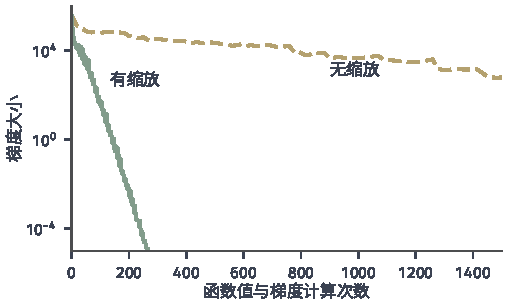
\includegraphics[width=86mm]{figures/05-optimization/02-smooth-optimization/matplotlib/qn-lbfgs-scaling/figure.pdf}
  \caption{初始缩放的影响：$r=10$，目标是$n=200$的旋转$\ln\cosh$函数（$c_i$在$[0.01,100]$上对数等距）再乘以$1000$，强Wolfe线搜索。绿线取式~\eqref{eq:qn-lbfgs-gamma}的缩放，黄虚线始终取$\gamma=1$。横轴是函数值与梯度的计算次数，纵轴是梯度大小。}
  \label{fig:qn-lbfgs-scaling}
\end{BookInlineFigure}

\section{收敛与计算成本}
\label{sec:qn-convergence}

前面各节展示了许多好现象，但例子都很小。于是要问：这些方法在什么条件下能保证什么？答案要分开说，因为不同的更新规则、线搜索和目标类型，对应的结论强弱不同。

全节的基本假设是：$f$二阶连续可微，存在$0<\mu\leq L$使$\mu\bm{I}\preceq\nabla^2f(\bm{x})\preceq L\bm{I}$对所有$\bm{x}$成立，$\bm{x}^\star$是唯一最优解。需要放宽时会明确说明。

\paragraph{一步下降与方向角}
先把线搜索的贡献算清楚。记$\theta^{(t)}$为$\bm{d}^{(t)}$与$-\bm{g}^{(t)}$的夹角，
\begin{equation}
 \cos\theta^{(t)}=\frac{-\langle\bm{g}^{(t)},\bm{d}^{(t)}\rangle}{\lVert\bm{g}^{(t)}\rVert_2\lVert\bm{d}^{(t)}\rVert_2}.
 \label{eq:qn-cos-theta}
\end{equation}
方向越接近负梯度，$\cos\theta^{(t)}$越接近$1$；方向几乎与梯度垂直时，它接近$0$，再好的步长也下降有限。

\begin{lemma}[Wolfe线搜索的一步下降]
\label{lem:qn-one-step}
设$\nabla f$是$L$-Lipschitz的，$\bm{d}^{(t)}$是下降方向，$\alpha^{(t)}$满足式~\eqref{eq:qn-wolfe}。则
\begin{equation}
 f(\bm{x}^{(t+1)})\leq f(\bm{x}^{(t)})-\frac{c_1(1-c_2)}{L}\cos^2\theta^{(t)}\lVert\bm{g}^{(t)}\rVert_2^2.
 \label{eq:qn-one-step}
\end{equation}
\end{lemma}

\begin{proof}
省略上标。由第二条Wolfe不等式和梯度的Lipschitz性，得到
\[
 (c_2-1)\langle\bm{g},\bm{d}\rangle\leq\langle\bm{g}^{+}-\bm{g},\bm{d}\rangle\leq\alpha L\lVert\bm{d}\rVert_2^2.
\]

这给出步长的下界：
\[
 \alpha\geq\frac{(1-c_2)\lvert\langle\bm{g},\bm{d}\rangle\rvert}{L\lVert\bm{d}\rVert_2^2}.
\]

把它代入第一条Wolfe不等式，并用式~\eqref{eq:qn-cos-theta}，得到
\[
 f(\bm{x}^{+})\leq f(\bm{x})-c_1\alpha\lvert\langle\bm{g},\bm{d}\rangle\rvert
 \leq f(\bm{x})-\frac{c_1(1-c_2)}{L}\cdot\frac{\langle\bm{g},\bm{d}\rangle^2}{\lVert\bm{d}\rVert_2^2},
\]
最后一个分式等于$\cos^2\theta\lVert\bm{g}\rVert_2^2$。
\end{proof}

把式~\eqref{eq:qn-one-step}对$t$求和，并用$f$有下界，就得到称为\term{Zoutendijk条件}（Zoutendijk condition）的结论$\sum_t\cos^2\theta^{(t)}\lVert\bm{g}^{(t)}\rVert_2^2<\infty$。所以只要$\cos\theta^{(t)}$不趋于零，梯度就要趋于零。全局收敛的问题变成：方向角能不能控制住？

\paragraph{BFGS的全局收敛}
BFGS的矩阵可能很差，方向可能很偏。下面的定理说，只要目标强凸，差的方向不可能一直出现。证明的工具是一个衡量矩阵“病态程度”的势函数，这也就是自校正的数学内容。

\begin{theorem}[BFGS在强凸目标上的全局收敛]
\label{thm:qn-bfgs-global}
设$f$满足本节的基本假设，$\bm{B}^{(0)}\succ\bm{0}$，步长满足Wolfe条件~\eqref{eq:qn-wolfe}，所有$\bm{g}^{(t)}\neq\bm{0}$。则BFGS的迭代点满足
\begin{equation}
 \lim_{t\to\infty}\bm{x}^{(t)}=\bm{x}^\star.
 \label{eq:qn-bfgs-global}
\end{equation}
\end{theorem}

\begin{proof}
由式~\eqref{eq:qn-wolfe-curvature}和定理~\ref{thm:qn-positive-definite}，所有$\bm{B}^{(t)}$正定。定义势函数
\[
 \psi(\bm{B})=\operatorname{tr}\bm{B}-\ln\det\bm{B}=\sum_{i=1}^n(\lambda_i-\ln\lambda_i),
\]
其中$\lambda_i$是$\bm{B}$的特征值。因为$\lambda-\ln\lambda\geq1$，所以$\psi(\bm{B})>0$。它同时惩罚过大和过小的特征值。

第一步，估计测量的尺度。省略上标，由式~\eqref{eq:qn-average-hessian}，并令$\bm{z}=\bar{\bm{H}}^{1/2}\bm{s}$，得到
\[
 \frac{\langle\bm{s},\bm{y}\rangle}{\langle\bm{s},\bm{s}\rangle}\geq\mu,\qquad
 \frac{\langle\bm{y},\bm{y}\rangle}{\langle\bm{s},\bm{y}\rangle}=\frac{\bm{z}^\top\bar{\bm{H}}\bm{z}}{\bm{z}^\top\bm{z}}\leq L.
\]

第二步，计算迹和行列式的变化。对式~\eqref{eq:qn-bfgs-direct}取迹，得到
\[
 \operatorname{tr}\bm{B}^{+}=\operatorname{tr}\bm{B}-\frac{\lVert\bm{B}\bm{s}\rVert_2^2}{\bm{s}^\top\bm{B}\bm{s}}+\frac{\lVert\bm{y}\rVert_2^2}{\langle\bm{s},\bm{y}\rangle}.
\]

行列式把$\bm{B}$提出来，写成
\[
 \det\bm{B}^{+}=\det\bm{B}\cdot\det\Bigl(\bm{I}-\frac{\bm{s}(\bm{B}\bm{s})^\top}{\bm{s}^\top\bm{B}\bm{s}}+\rho\,\bm{W}\bm{y}\bm{y}^\top\Bigr).
\]
括号内是$\bm{I}+\bm{U}\bm{C}^\top$的形式，其中$\bm{U}$的两列是$-\bm{s}/(\bm{s}^\top\bm{B}\bm{s})$与$\rho\bm{W}\bm{y}$，$\bm{C}$的两列是$\bm{B}\bm{s}$与$\bm{y}$。由行列式的恒等式（交换乘积因子，维数从$n$降到$2$），$\bm{I}+\bm{U}\bm{C}^\top$与$\bm{I}+\bm{C}^\top\bm{U}$的行列式相同。沿用第~\ref{sec:qn-dfp-bfgs}节的曲率比$\tau$，则
\[
 \bm{I}+\bm{C}^\top\bm{U}=\begin{bmatrix}0&1\\-\tau&1+\rho\,\bm{y}^\top\bm{W}\bm{y}\end{bmatrix},
\]
这个矩阵的行列式是$\tau$，因此
\[
 \det\bm{B}^{+}=\det\bm{B}\cdot\frac{\langle\bm{s},\bm{y}\rangle}{\bm{s}^\top\bm{B}\bm{s}}.
\]

第三步，用方向角重写。由$\bm{B}\bm{d}=-\bm{g}$和$\bm{s}=\alpha\bm{d}$，式~\eqref{eq:qn-cos-theta}的夹角满足
\[
 \cos\theta=\frac{\bm{s}^\top\bm{B}\bm{s}}{\lVert\bm{s}\rVert_2\lVert\bm{B}\bm{s}\rVert_2}.
\]

再引入三个比值：
\[
 q=\frac{\bm{s}^\top\bm{B}\bm{s}}{\langle\bm{s},\bm{s}\rangle},\qquad m_{\mathrm{c}}=\frac{\langle\bm{s},\bm{y}\rangle}{\langle\bm{s},\bm{s}\rangle},\qquad M_{\mathrm{c}}=\frac{\langle\bm{y},\bm{y}\rangle}{\langle\bm{s},\bm{y}\rangle}.
\]
于是迹和行列式公式中的两个量可以写成
\[
 \frac{\lVert\bm{B}\bm{s}\rVert_2^2}{\bm{s}^\top\bm{B}\bm{s}}=\frac{q}{\cos^2\theta},\qquad
 \frac{\langle\bm{s},\bm{y}\rangle}{\bm{s}^\top\bm{B}\bm{s}}=\frac{m_{\mathrm{c}}}{q}.
\]

把第二步的结果代入$\psi$，整理得到
\[
 \psi(\bm{B}^{+})=\psi(\bm{B})+(M_{\mathrm{c}}-\ln m_{\mathrm{c}}-1)
 +\Bigl[1-\frac{q}{\cos^2\theta}+\ln\frac{q}{\cos^2\theta}\Bigr]+\ln\cos^2\theta.
\]
方括号非正，因为$1-v+\ln v\leq0$对$v>0$成立。令$c=\max\{L-\ln\mu-1,\,1\}>0$，由第一步，
\[
 \psi(\bm{B}^{(t+1)})\leq\psi(\bm{B}^{(0)})+c(t+1)+\sum_{j=0}^{t}\ln\cos^2\theta^{(j)}.
\]

第四步，反证。设$\cos\theta^{(t)}\to0$，则存在$t_1$，当$j>t_1$时$\ln\cos^2\theta^{(j)}<-2c$。对$t>t_1$，上式右端不超过
\[
 \psi(\bm{B}^{(0)})+c(t+1)+\sum_{j\leq t_1}\ln\cos^2\theta^{(j)}-2c(t-t_1).
\]
它随$t$线性趋于$-\infty$，与$\psi>0$矛盾。所以存在$\delta>0$和子列使$\cos\theta^{(t)}\geq\delta$。

第五步，收敛。对引理~\ref{lem:qn-one-step}求和，得到Zoutendijk条件，所以沿这个子列$\lVert\bm{g}^{(t)}\rVert_2\to0$。第~\ref{chap:optimization}章的误差换算给出下面两个不等式：
\[
 f(\bm{x})-f^\star\leq\frac{\lVert\nabla f(\bm{x})\rVert_2^2}{2\mu},\qquad
 \frac{\mu}{2}\lVert\bm{x}-\bm{x}^\star\rVert_2^2\leq f(\bm{x})-f^\star.
\]
前一个说明沿子列$f(\bm{x}^{(t)})\to f^\star$。

$f(\bm{x}^{(t)})$单调，于是整个序列的目标值都收敛到$f^\star$。再由后一个不等式，迭代点收敛到$\bm{x}^\star$。
\end{proof}

用贯穿例的BFGS（$\bm{B}^{(0)}=\bm{I}$，精确线搜索）核对一下这个公式。三个矩阵的$\psi$值是
\[
 \begin{gathered}
 \psi(\bm{B}^{(0)})=2,\qquad\psi(\bm{B}^{(1)})=7.8-\ln5\approx6.191,\\
 \psi(\bm{B}^{(2)})=10-\ln16\approx7.227.
 \end{gathered}
\]

第一次更新$\cos\theta^{(0)}=1$、$q=1$，方括号与最后的对数都是零，增量全部来自尺度项。按定理证明中的记号，$M_{\mathrm{c}}=6.8$，$m_{\mathrm{c}}=5$，于是
\[
 \psi(\bm{B}^{(1)})-\psi(\bm{B}^{(0)})=6.8-\ln5-1\approx4.191.
\]

第二次更新的方向角满足$\cos^2\theta^{(1)}\approx0.735$，此时$q/\cos^2\theta^{(1)}=1$，方括号仍是零。尺度项是$3.2-\ln2.353-1\approx1.344$，而$\ln\cos^2\theta^{(1)}\approx-0.308$，两者之和与$\psi$的实际增量$1.036$一致。

定理的证明解释了自校正：$\psi$每一步至多增加一个常数，而每次方向偏得厉害都要付出$\ln\cos^2\theta$这一项的大幅减少，方向不可能一直偏。证明中的第二步用到了BFGS特有的迹和行列式公式，不能搬给DFP；我们也不声称DFP在Wolfe线搜索下有同样的结论，图~\ref{fig:qn-dfp-bfgs-scaling}(b)显示它确实可能很慢。

对一般非凸目标，没有类似的定理：已有构造性例子说明，即使线搜索满足Wolfe条件，BFGS也可能不收敛到驻点。实践中BFGS常常工作良好，但这不是定理所保证的。

\paragraph{局部收敛的刻画：Dennis--Moré条件}
全局收敛说的是终将到达，还要看到达的速度。称$\bm{x}^{(t)}\to\bm{x}^\star$是\term{超线性收敛}（superlinear convergence），如果
\begin{equation}
 \lim_{t\to\infty}\frac{\lVert\bm{x}^{(t+1)}-\bm{x}^\star\rVert_2}{\lVert\bm{x}^{(t)}-\bm{x}^\star\rVert_2}=0.
 \label{eq:qn-superlinear}
\end{equation}
Newton法靠的是矩阵趋于Hessian。拟牛顿矩阵一般并不趋于Hessian，超线性收敛却仍然可能发生。下面的定理说明，真正需要的只是沿步方向准确。

\begin{theorem}[Dennis--Moré特征]
\label{thm:qn-dennis-more}
设$f$二阶连续可微，$\bm{x}^{(t)}\to\bm{x}^\star$，$\bm{x}^\star$是驻点，$\bm{H}^\star=\nabla^2f(\bm{x}^\star)$正定。设对充分大的$t$，迭代取单位步长且方向$\bm{d}^{(t)}\neq\bm{0}$由$\bm{B}^{(t)}\bm{d}^{(t)}=-\bm{g}^{(t)}$确定。则序列超线性收敛，当且仅当
\begin{equation}
 \lim_{t\to\infty}\frac{\lVert(\bm{B}^{(t)}-\bm{H}^\star)\bm{d}^{(t)}\rVert_2}{\lVert\bm{d}^{(t)}\rVert_2}=0.
 \label{eq:qn-dennis-more}
\end{equation}
\end{theorem}

\begin{proof}
省略上标，把误差写成$\bm{e}=\bm{x}-\bm{x}^\star$、$\bm{e}^{+}=\bm{x}^{+}-\bm{x}^\star$。与式~\eqref{eq:qn-average-hessian}一样，梯度差等于平均Hessian乘$\bm{d}$。代入$\bm{g}=-\bm{B}\bm{d}$，得到关键等式
\[
 \bm{g}^{+}=(\bar{\bm{H}}-\bm{H}^\star)\bm{d}+(\bm{H}^\star-\bm{B})\bm{d}.
\]
因为$\bm{x}^{(t)}\to\bm{x}^\star$且Hessian连续，所以$\bar{\bm{H}}\to\bm{H}^\star$，第一项是$o(\lVert\bm{d}\rVert_2)$。

充分性：设式~\eqref{eq:qn-dennis-more}成立，则$\lVert\bm{g}^{+}\rVert_2=o(\lVert\bm{d}\rVert_2)$。在$\bm{x}^\star$附近，$\nabla^2f$的最小特征值不小于某个$\mu_{\star}>0$，所以
\[
 \lVert\bm{g}^{+}\rVert_2\geq\mu_{\star}\lVert\bm{e}^{+}\rVert_2.
\]

再由三角不等式，$\lVert\bm{d}\rVert_2$不超过两个误差的范数之和，于是
\[
 \lVert\bm{e}^{+}\rVert_2\leq o(1)\bigl(\lVert\bm{e}\rVert_2+\lVert\bm{e}^{+}\rVert_2\bigr).
\]
移项即得$\lVert\bm{e}^{+}\rVert_2=o(\lVert\bm{e}\rVert_2)$。

必要性：设序列超线性收敛。由三角不等式，$\lVert\bm{d}\rVert_2$不小于$\lVert\bm{e}\rVert_2-\lVert\bm{e}^{+}\rVert_2$，而$\lVert\bm{e}^{+}\rVert_2=o(\lVert\bm{e}\rVert_2)$，于是$\lVert\bm{e}\rVert_2=O(\lVert\bm{d}\rVert_2)$。

$\nabla f$在$\bm{x}^\star$处为零且连续可微，所以$\lVert\bm{g}^{+}\rVert_2$是$\lVert\bm{e}^{+}\rVert_2$的同阶小量，于是
\[
 \lVert\bm{g}^{+}\rVert_2=o(\lVert\bm{e}\rVert_2)=o(\lVert\bm{d}\rVert_2).
\]
由关键等式解出第二项，并用$\bar{\bm{H}}\to\bm{H}^\star$，得到式~\eqref{eq:qn-dennis-more}。
\end{proof}

式~\eqref{eq:qn-dennis-more}称为\term{Dennis--Moré条件}（Dennis--Moré condition）。它只比较矩阵在搜索方向上的作用，所以拟牛顿矩阵不必收敛到Hessian。图~\ref{fig:qn-rates}(b)印证了这一点：迭代结束时矩阵整体的误差约为$3\%$，沿步方向的误差约为$0.08\%$。

定理假设步长最终是$1$。满足式~\eqref{eq:qn-dennis-more}且$c_1<1/2$时，Wolfe线搜索最终确实接受单位步长，证明可查阅\scite{math-nocedal2006numerical}。这也是线搜索要优先试$\alpha=1$的理由：如果不试，或者试了又不接受，上面的超线性机制就用不上。

\paragraph{BFGS的超线性收敛}
完整记忆的BFGS确实满足Dennis--Moré条件，但需要更强的正则性。若$\bm{x}^{(t)}\to\bm{x}^\star$，$\bm{H}^\star$正定，$\nabla^2f$在$\bm{x}^\star$附近Lipschitz连续，且$\sum_t\lVert\bm{x}^{(t)}-\bm{x}^\star\rVert_2<\infty$，又有单位步长优先试探的线搜索，则BFGS超线性收敛。

证明要沿用定理~\ref{thm:qn-bfgs-global}的势函数并在$\bm{H}^\star$定义的坐标下估计，篇幅较长，读者可查阅\scite{math-nocedal2006numerical}。求和条件要求误差足够快地衰减，在定理~\ref{thm:qn-bfgs-global}的强凸条件下可以进一步证明它成立。Lipschitz条件的作用是控制$\bar{\bm{H}}^{(t)}$与$\bm{H}^\star$之差，使测量误差可以累加。

\begin{BookInlineFigure}
  \centering
  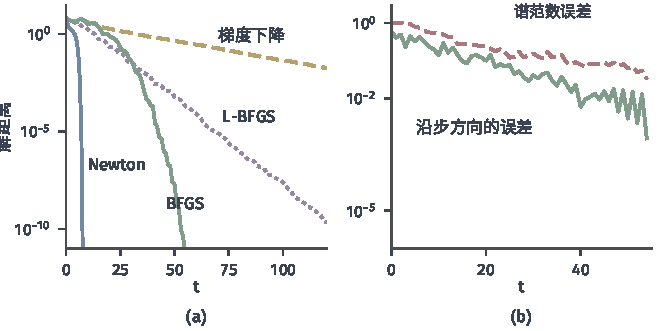
\includegraphics[width=112mm]{figures/05-optimization/02-smooth-optimization/matplotlib/qn-rates/figure.pdf}
  \caption{不同方法的局部速度，目标是$50$维的旋转$\ln\cosh$函数（$c_i$在$[0.1,100]$上对数等距，$\bm{x}^\star=\bm{0}$），强Wolfe线搜索。(a)解距离随迭代的变化：梯度下降（黄虚线）线性且慢，$r=5$的L-BFGS（紫点线）线性，BFGS（绿）后期斜率变陡，Newton法（蓝）最快。(b)BFGS的矩阵相对误差：红虚线是$\lVert\bm{B}^{(t)}-\bm{H}^\star\rVert_2/\lVert\bm{H}^\star\rVert_2$，绿线是Dennis--Moré比值$\lVert(\bm{B}^{(t)}-\bm{H}^\star)\bm{s}^{(t)}\rVert_2/(\lVert\bm{H}^\star\rVert_2\lVert\bm{s}^{(t)}\rVert_2)$。}
  \label{fig:qn-rates}
\end{BookInlineFigure}

\paragraph{SR1的局部结论}
SR1的结论需要不同的条件，第~\ref{sec:qn-sr1}节的定理只覆盖二次目标。对一般目标，已有的结果大致是：在$\bm{H}^\star$正定、分母保持远离零、步方向具有一致线性无关性质时，$\bm{B}^{(t)}$本身收敛到Hessian，配合信赖域可得到$n+1$步意义下的超线性收敛。这些条件比BFGS的条件更难事先验证，也不能换成Wolfe线搜索下的方向分析；相应证明见\scite{math-nocedal2006numerical}。

\paragraph{L-BFGS只保证线性收敛}
完整BFGS的超线性结论不能自动移给固定记忆的L-BFGS。超线性机制要求矩阵逐渐掌握沿步方向的曲率，而每轮重新从$\gamma\bm{I}$开始、只用$r$对向量的矩阵，无法累积足够的信息。下面的定理给出固定记忆下能证明的保证。

\begin{theorem}[L-BFGS的线性收敛]
\label{thm:qn-lbfgs-linear}
设$f$满足本节的基本假设，$t\geq1$时$\gamma^{(t)}$由式~\eqref{eq:qn-lbfgs-gamma}给出，$t=0$时取负梯度方向，记忆长度为$r$，步长满足Wolfe条件。令$T_{\mathrm{c}}=(n+r)L$，$\delta=(\mu/T_{\mathrm{c}})^{n+r}$。则
\begin{equation}
 f(\bm{x}^{(t+1)})-f^\star\leq\Bigl(1-\frac{2\mu c_1(1-c_2)\delta^2}{L}\Bigr)\bigl(f(\bm{x}^{(t)})-f^\star\bigr).
 \label{eq:qn-lbfgs-linear}
\end{equation}
\end{theorem}

\begin{proof}
设$\bm{B}_{[j]}=\bm{W}_{[j]}^{-1}$，它们由$\bm{B}_{[t-r]}=(1/\gamma^{(t)})\bm{I}$出发，按BFGS的直接形式更新$r$次。第一步，由定理~\ref{thm:qn-bfgs-global}证明中的尺度估计，$1/\gamma^{(t)}\in[\mu,L]$。

第二步，约束迹。式~\eqref{eq:qn-bfgs-direct}的修正中，减去的一项迹非负，加上的一项迹不超过$L$，于是
\[
 \operatorname{tr}\bm{B}_{[t]}\leq\frac{n}{\gamma^{(t)}}+rL\leq(n+r)L=T_{\mathrm{c}}.
\]
所以每个$\bm{B}_{[j]}$的最大特征值不超过$T_{\mathrm{c}}$。

第三步，约束行列式。由行列式公式和第一步，每次更新满足
\[
 \frac{\det\bm{B}_{[j+1]}}{\det\bm{B}_{[j]}}=\frac{\langle\bm{s},\bm{y}\rangle}{\bm{s}^\top\bm{B}_{[j]}\bm{s}}\geq\frac{\mu\lVert\bm{s}\rVert_2^2}{T_{\mathrm{c}}\lVert\bm{s}\rVert_2^2}=\frac{\mu}{T_{\mathrm{c}}}.
\]
连乘至多$r$次（窗口未满时次数更少，因$\mu/T_{\mathrm{c}}\leq1$，下界不变），并用$\det\bm{B}_{[t-r]}\geq\mu^n$，得到
\[
 \det\bm{B}^{(t)}\geq\mu^n\Bigl(\frac{\mu}{T_{\mathrm{c}}}\Bigr)^r.
\]

第四步，约束方向角。最小特征值至少是行列式除以另外$n-1$个特征值的上界，所以$\bm{B}^{(t)}$的条件数不超过
\[
 \frac{T_{\mathrm{c}}^{\,n}}{\det\bm{B}^{(t)}}\leq\Bigl(\frac{T_{\mathrm{c}}}{\mu}\Bigr)^{n+r}=\frac{1}{\delta}.
\]

由$\bm{d}=-\bm{W}\bm{g}$，方向角满足
\[
 \cos\theta^{(t)}=\frac{\bm{g}^\top\bm{W}\bm{g}}{\lVert\bm{g}\rVert_2\lVert\bm{W}\bm{g}\rVert_2}\geq\frac{\lambda_{\min}(\bm{W})}{\lambda_{\max}(\bm{W})}\geq\delta.
\]

第五步，代入引理~\ref{lem:qn-one-step}，并用第~\ref{chap:optimization}章的$\lVert\bm{g}\rVert_2^2\geq2\mu(f-f^\star)$，即得式~\eqref{eq:qn-lbfgs-linear}。
\end{proof}

定理的常数$\delta$随$n+r$指数变小，几乎没有定量价值。它的意义在于定性：固定记忆时，矩阵的条件数有界，因而线性收敛，且这个结论不依赖超线性的机制。图~\ref{fig:qn-rates}(a)中L-BFGS的直线正是线性收敛的样子，实际的速度远比定理的常数好。

\paragraph{各方法的保证}
下表汇总本节的结论，列出的是使结论成立的条件，并非全部的可行条件。

\begin{BookInlineTable}
  \centering
  \small
  \begin{tabular}{p{15mm}p{39mm}p{39mm}}
    \toprule
    方法 & 全局 & 局部\\
    \midrule
    BFGS & 强凸＋Wolfe：收敛（已证） & Hessian Lipschitz、误差可和：超线性\\
    DFP & 本章的势函数论证不适用 & 不作结论\\
    SR1 & 二次目标：至多$n+1$步（已证） & 分母与步方向条件＋信赖域：$n+1$步意义下超线性\\
    L-BFGS & 强凸＋Wolfe：线性收敛（已证） & 不保证超线性\\
    \bottomrule
  \end{tabular}
  \caption{拟牛顿方法的收敛保证汇总。}
  \label{tab:qn-guarantees}
\end{BookInlineTable}

\paragraph{计算成本}
比较成本要固定相同的精度，并把各项都算上。下表列出每一步除梯度外的开销，$n$是变量维数，$r$是记忆长度，线搜索的函数和梯度计算次数另算。

\begin{BookInlineTable}
  \centering
  \begin{tabular}{lll}
    \toprule
    方法 & 存储 & 方向与更新的乘法次数\\
    \midrule
    梯度下降 & $n$ & $n$\\
    L-BFGS & $2rn$ & $(4r+1)n$\\
    BFGS、DFP、SR1 & $n^2/2$ & 约$4n^2$\\
    Newton法 & $n^2/2$ & 约$n^3/3$，另加形成Hessian\\
    \bottomrule
  \end{tabular}
  \caption{每步除梯度以外的存储与运算，Newton法按Cholesky分解计。}
  \label{tab:qn-cost}
\end{BookInlineTable}

单步开销低的方法不一定总开销低，要乘上迭代数才能比较。图~\ref{fig:qn-rates}的目标取$n=50$，达到解距离$10^{-8}$需要的迭代数和方向运算量如表~\ref{tab:qn-experiment-cost}所示。

\begin{BookInlineTable}
  \centering
  \begin{tabular}{lrrr}
    \toprule
    方法 & 迭代数 & 每步方向运算 & 方向运算合计\\
    \midrule
    梯度下降 & $458$ & $50$ & $2.3\times10^{4}$\\
    L-BFGS（$r=5$） & $104$ & $1050$ & $1.1\times10^{5}$\\
    BFGS & $51$ & $1.0\times10^{4}$ & $5.1\times10^{5}$\\
    Newton法 & $8$ & $4.2\times10^{4}$ & $3.3\times10^{5}$\\
    \bottomrule
  \end{tabular}
  \caption{图~\ref{fig:qn-rates}的目标（$n=50$）上达到解距离$10^{-8}$的迭代数与方向运算量，不含梯度和Hessian的计算。}
  \label{tab:qn-experiment-cost}
\end{BookInlineTable}

这张表不能单独读。这个目标上一次梯度要做两次$50\times50$的矩阵乘法，约$5000$次运算，所以梯度下降实际花在梯度上的开销约为$2.3\times10^{6}$，远超方向运算本身。Newton法的Hessian开销未计入；在$n=50$时分解很便宜，$n$增大后三次方项才成为主要矛盾。比较的结论要在实际的$n$、梯度和Hessian成本下重新算。

实际选择大致如下：$n$不大、梯度贵、要高精度时用完整BFGS；$n$很大时用L-BFGS，代价是只有线性速度的保证；需要负曲率信息时用SR1配信赖域。

\section{本章小结}
\label{sec:qn-summary}

本章开头的问题是：Hessian算不起、存不下时，能否从迭代本身得到曲率信息。答案是相邻两点的梯度差。式~\eqref{eq:qn-average-hessian}说明它是平均Hessian作用在位移上的结果，由此得到割线条件。这个条件在$n=1$时确定了曲率，$n>1$时还缺$n(n-1)/2$个方程，所以需要补充对称、低秩和曲率的要求。

不同的补充要求产生了不同的方法。DFP和BFGS各用两个秩一项，分别在矩阵和逆矩阵上度量改动。两者都在曲率条件$\langle\bm{s},\bm{y}\rangle>0$下保持正定，Wolfe线搜索使这个条件对任意光滑目标成立，跳过和阻尼是线搜索之外的备用办法。

SR1只用一个秩一项，由割线条件唯一确定。它在二次目标上有更强的遗传性质，能记录负曲率，但分母可能近零，矩阵也可能不定，所以需要跳过规则，且方向分析不能照搬，要交给有界的模型处理。

L-BFGS用双循环递推在不保存矩阵的情况下计算$\bm{W}^{(t)}\bm{g}^{(t)}$，把存储从$n^2/2$降到$2rn$。记忆长度决定了方向的质量和每步的计算量，初始缩放决定了单位步长是否合适。

\begin{BookInlineTable}
  \centering
  \begin{tabular}{llll}
    \toprule
    方法 & 新增信息 & 保持的性质 & 单步主要开销\\
    \midrule
    BFGS & 秩二修正 & 曲率条件下正定 & $O(n^2)$\\
    DFP & 秩二修正 & 曲率条件下正定 & $O(n^2)$\\
    SR1 & 秩一修正 & 可表示负曲率 & $O(n^2)$\\
    L-BFGS & 最近$r$对 & 曲率条件下正定 & $O(rn)$\\
    \bottomrule
  \end{tabular}
  \caption{本章四种拟牛顿方法的比较。}
  \label{tab:qn-summary}
\end{BookInlineTable}

收敛结论要分开看。BFGS在强凸目标和Wolfe线搜索下全局收敛，在更强的正则性下超线性收敛，后者由Dennis--Mor\'e条件刻画，它只要求沿步方向准确。L-BFGS在强凸目标上线性收敛，完整记忆的超线性结论不能自动移给它。一般非凸目标上，这些保证都不成立，SR1在一般目标上的局部结论也有额外条件。

拟牛顿矩阵的好坏，最终还要看模型在多大范围内可信。线搜索只沿一个方向试探，不定模型又没有极小点；第~\ref{chap:trust-region}章研究的信赖域，把候选步和接受判断放在一起处理，并且既可以用精确Hessian，也可以用本章的拟牛顿矩阵。


\chapter{信赖域}
\label{chap:trust-region}

站在一个点上，手里有目标的梯度和曲率，可以写出一个二次模型，模型的最小点似乎就是下一步该去的地方。可是模型只是在当前点附近展开得到的，走远了它就可能完全失真；曲率不正定时，模型甚至没有最小点。第~\ref{chap:smooth-foundations}章的线搜索先定方向、再定步长，方向一旦定错，步长再怎么调也救不回来。

本章换一个顺序：先问“模型能信多远”，在这个范围内求模型的最小点，方向和长度一起决定，再用真实目标检验模型预测得准不准，据此调整下一轮的范围。这样得到的方法叫\term{信赖域}（trust region）方法。

全章用同一个二维目标把这件事算到底。先写出子问题，看清它的解长什么样；再比较三种便宜的近似求解办法；然后组织完整的迭代，看一步被拒绝时发生什么；最后讨论这套做法能保证什么、不能保证什么，以及它的计算代价。

\section{信赖域模型}
\label{sec:tr-model}

既然局部模型只在一定范围内可靠，怎样把“只在这个范围内相信它”写成一个可以计算的问题？

\paragraph{贯穿全章的例子}
我们用下面这个二维目标：
\begin{equation}
 f(\bm{x})=\frac14x_1^4-\frac12x_1^2+x_1+\frac32x_2^2+x_2.
 \label{eq:tr-example}
\end{equation}
它的梯度和Hessian可以直接写出：
\begin{equation}
 \nabla f(\bm{x})=\begin{bmatrix}x_1^3-x_1+1\\3x_2+1\end{bmatrix},\qquad
 \nabla^2 f(\bm{x})=\begin{bmatrix}3x_1^2-1&0\\0&3\end{bmatrix}.
 \label{eq:tr-example-derivatives}
\end{equation}

令梯度为零，第二个分量给出$x_2=-1/3$，第一个分量是三次方程$x_1^3-x_1+1=0$，它只有一个实根$x_1\approx-1.3247$。这个驻点处Hessian正定，$f$又随$\lVert\bm{x}\rVert_2\to\infty$趋于正无穷，所以它就是全局最小点：
\[
 \bm{x}^\star\approx(-1.3247,\,-0.3333)^\top,\qquad f^\star\approx-1.5989.
\]

全章反复用到两个点。一个是$\bm{a}=(2,2)^\top$，这里Hessian正定，数据是
\begin{equation}
 f(\bm{a})=12,\qquad \bm{g}=\begin{bmatrix}7\\7\end{bmatrix},\qquad \bm{B}=\begin{bmatrix}11&0\\0&3\end{bmatrix}.
 \label{eq:tr-data-a}
\end{equation}
另一个是原点，这里Hessian不定，数据是
\begin{equation}
 f(\bm{0})=0,\qquad \bm{g}=\begin{bmatrix}1\\1\end{bmatrix},\qquad \bm{B}=\begin{bmatrix}-1&0\\0&3\end{bmatrix}.
 \label{eq:tr-data-o}
\end{equation}

\paragraph{模型能信多远}
在当前点$\bm{x}^{(t)}$展开到二阶，用位移$\bm{p}$作自变量，就得到\term{二次模型}（quadratic model）：
\begin{equation}
 m^{(t)}(\bm{p})=f(\bm{x}^{(t)})+\langle\bm{g}^{(t)},\bm{p}\rangle+\frac12\bm{p}^\top\bm{B}^{(t)}\bm{p}.
 \label{eq:tr-model}
\end{equation}
其中$\bm{g}^{(t)}=\nabla f(\bm{x}^{(t)})$，$\bm{B}^{(t)}$是对称矩阵，可以取Hessian $\bm{H}^{(t)}$，也可以取第~\ref{chap:quasi-newton}章由梯度差构造的近似。本节取$\bm{B}^{(t)}=\bm{H}^{(t)}$。

模型与目标差多少？例中$x_2$部分本来就是二次的，没有误差；$x_1$部分由四次多项式的展开直接得到，当$\bm{B}$取Hessian时
\begin{equation}
 f(\bm{x}+\bm{p})-m(\bm{p})=x_1p_1^3+\frac14p_1^4.
 \label{eq:tr-example-error}
\end{equation}

误差随$\lvert p_1\rvert$的增大而迅速增大。$\lvert p_1\rvert$很小时，高阶项微不足道；$\lvert p_1\rvert$到了$2$，在原点误差就是$4$，已经超过这里函数值变化的量级。图~\ref{fig:tr-model-slice}沿$x_1$方向画出了这件事，浅蓝带表示模型大致可信的范围。

\begin{BookInlineFigure}
 \centering
 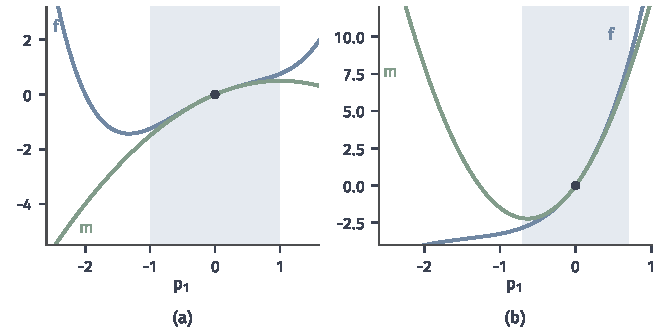
\includegraphics[width=112mm]{figures/05-optimization/02-smooth-optimization/matplotlib/tr-model-slice/figure.pdf}
 \caption{目标~\eqref{eq:tr-example}的$x_1$部分（蓝）与二次模型（绿）沿$p_1$的比较，黑点是展开点，浅蓝带是两者大致重合的范围。(a)~在$x_1=0$展开，曲率为负，模型向左无限下降，而目标很快转头向上。(b)~在$x_1=2$展开，曲率为正，模型有最小点，但左侧的目标比模型低得多。}
 \label{fig:tr-model-slice}
\end{BookInlineFigure}

图~\ref{fig:tr-model-contours}在平面上比较同一件事。在点$\bm{a}$附近，两组等高线几乎一样；离开圆盘之后，目标的等高线向左拉伸，模型仍是一组椭圆。

\begin{BookInlineFigure}
 \centering
 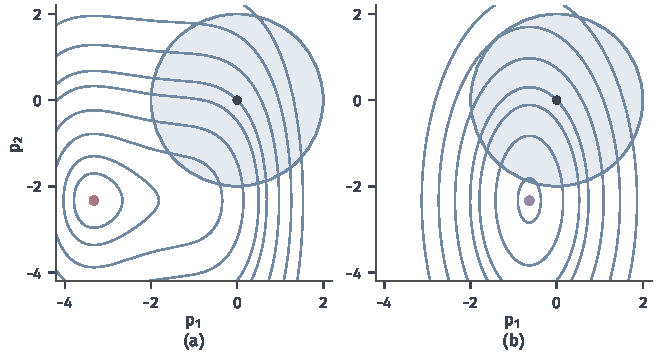
\includegraphics[width=112mm]{figures/05-optimization/02-smooth-optimization/matplotlib/tr-model-contours/figure.pdf}
 \caption{以$\bm{a}=(2,2)^\top$为原点的位移坐标下的等高线（蓝）。(a)~真实目标，红点是最小点。(b)~二次模型，紫点是模型的最小点。浅蓝圆盘半径为$2$，圆盘内两图相近，圆盘外差别明显。}
 \label{fig:tr-model-contours}
\end{BookInlineFigure}

\paragraph{子问题}
既然模型只在附近可靠，就只在附近找它的最小点。给定半径$\Delta^{(t)}>0$，定义\term{信赖域子问题}（trust-region subproblem）：
\begin{equation}
 \min_{\bm{p}\in\mathbb{R}^n}\ m^{(t)}(\bm{p})\qquad\text{满足}\quad\lVert\bm{p}\rVert_2\leq\Delta^{(t)}.
 \label{eq:tr-subproblem}
\end{equation}
半径$\Delta^{(t)}$约束的是这一轮的位移，原问题仍然是无约束的。下一轮换一个点、换一个半径，约束也跟着换。

半径的含义可以用一张手绘地图来理解。地图是在当前位置附近勘测的（对应二次模型），周围画得准，远处多半是推测。你决定只按地图走到某个距离为止（对应半径），走到后核对实地与地图是否相符，相符就下次敢走远些，不符就走近些（对应后面的半径更新）。这个类比有一处不贴切：半径并不是模型真实误差的边界，它只是算法根据最近的核对结果作出的估计，可能偏大，也可能偏小。

\paragraph{曲率不正定时}
第~\ref{chap:second-order-methods}章的Newton法要解$\bm{B}\bm{d}=-\bm{g}$。原点的数据~\eqref{eq:tr-data-o}上这个方程仍可解，解是
\[
 \bm{d}^{\mathrm{N}}=-\bm{B}^{-1}\bm{g}=\begin{bmatrix}1\\-1/3\end{bmatrix}.
\]

它与梯度的内积决定这个方向是上坡还是下坡：
\[
 \langle\bm{g},\bm{d}^{\mathrm{N}}\rangle=1-\frac13=\frac23>0.
\]
内积为正，这个方向是上坡方向。$\bm{d}^{\mathrm{N}}$只是模型的驻点，模型在这里是个鞍面。沿$\bm{d}^{\mathrm{N}}$作线搜索不会有任何下降的步长，所以线搜索框架不得不先修改$\bm{B}$，使它正定。

信赖域子问题没有这个麻烦。闭球是紧集，$m$连续，所以无论$\bm{B}$是否正定，最小点都存在。例中模型沿$p_1$轴是$p_1-p_1^2/2$，向左无限下降，无约束时没有最小点；加上半径之后，解就落在球的边界上。图~\ref{fig:tr-newton-ascent}画出了$\Delta=2$的情形：$\bm{B}$无需修改，负曲率反而被利用，它把解推向了边界。

\begin{BookInlineFigure}
 \centering
 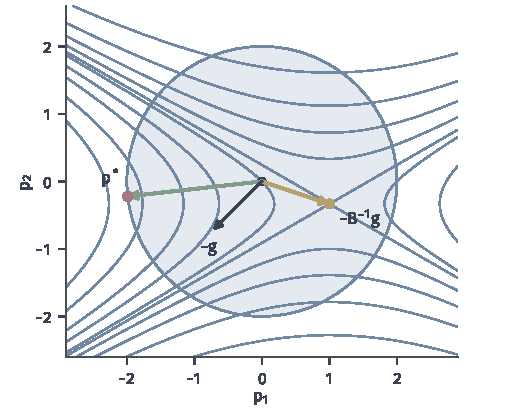
\includegraphics[width=88mm]{figures/05-optimization/02-smooth-optimization/matplotlib/tr-newton-ascent/figure.pdf}
 \caption{原点处的二次模型，蓝线是等高线，浅蓝圆盘半径$\Delta=2$。黄色箭头指向模型的驻点$-\bm{B}^{-1}\bm{g}$，黑色箭头是负梯度方向，红点是子问题的全局解$\bm{p}^\star$，绿色箭头指向它。黄色方向是上坡方向，而子问题的解利用负曲率走到了圆盘左侧边界。}
 \label{fig:tr-newton-ascent}
\end{BookInlineFigure}

\paragraph{与线搜索的对照}
第~\ref{chap:smooth-foundations}章的线搜索分两步：先选定下降方向$\bm{d}^{(t)}$，再沿这条射线选步长$\alpha^{(t)}$。信赖域把顺序倒过来：先选定半径，再同时决定方向和长度。半径变了，步的方向也跟着变。

在点$\bm{a}$，图~\ref{fig:tr-line-vs-region}画出了两者的差别。线搜索的候选点都在一条射线上；信赖域的解随半径变化走出一条曲线，半径小时贴近负梯度方向，半径大时转向Newton点。半径的调整因此比步长的调整多一层作用，它还在改变方向。

\begin{BookInlineFigure}
 \centering
 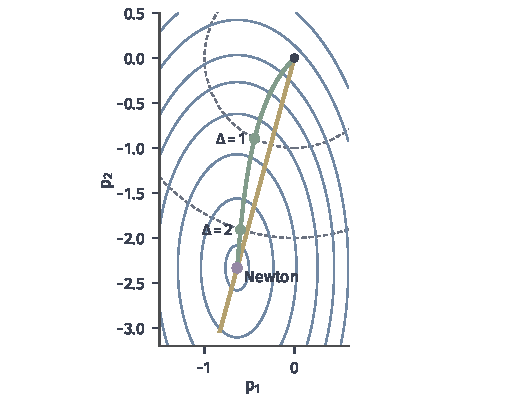
\includegraphics[width=86mm]{figures/05-optimization/02-smooth-optimization/matplotlib/tr-line-vs-region/figure.pdf}
 \caption{点$\bm{a}$处的二次模型等高线（蓝）。黄线是沿Newton方向的射线，线搜索只在这条线上选点。绿线是子问题的全局解随$\Delta$变化的轨迹，绿点是$\Delta=1$和$\Delta=2$时的解，虚线圆是对应的边界，紫点是Newton点。}
 \label{fig:tr-line-vs-region}
\end{BookInlineFigure}

表~\ref{tab:tr-vs-linesearch}把两种做法并列。

\begin{BookInlineTable}
 \centering
 \begin{tabular}{lll}
  \toprule
  & 线搜索 & 信赖域\\
  \midrule
  先固定的量 & 方向$\bm{d}^{(t)}$ & 半径$\Delta^{(t)}$\\
  后决定的量 & 步长$\alpha^{(t)}$ & 位移$\bm{p}^{(t)}$（方向和长度）\\
  $\bm{B}$的要求 & 需要给出下降方向 & 对称即可\\
  一次试探失败 & 缩短步长，方向不变 & 缩小半径，方向可变\\
  \bottomrule
 \end{tabular}
 \caption{线搜索与信赖域的分工对照。}
 \label{tab:tr-vs-linesearch}
\end{BookInlineTable}

\paragraph{子问题的全局解}
子问题虽然非凸，它的全局解却有干净的刻画。下面的定理说明，解满足一个被平移过的线性方程，平移量$\lambda$恰好使矩阵半正定。

\begin{theorem}[子问题的全局解]
 \label{thm:tr-exact}
 设$\bm{B}$对称，$\Delta>0$，$m$如式~\eqref{eq:tr-model}（省略上标$(t)$）。点$\bm{p}^\star$是子问题~\eqref{eq:tr-subproblem}的全局解，当且仅当$\lVert\bm{p}^\star\rVert_2\leq\Delta$，并且存在$\lambda\geq0$，使得
 \begin{equation}
  (\bm{B}+\lambda\bm{I})\bm{p}^\star=-\bm{g},\qquad
  \lambda(\Delta-\lVert\bm{p}^\star\rVert_2)=0,\qquad
  \bm{B}+\lambda\bm{I}\succeq\bm{0}.
  \label{eq:tr-exact-conditions}
 \end{equation}
\end{theorem}

\begin{proof}
 先证充分性。令
 \[
  \hat{m}(\bm{p})=m(\bm{p})+\frac{\lambda}{2}\lVert\bm{p}\rVert_2^2.
 \]
 它的Hessian是$\bm{B}+\lambda\bm{I}\succeq\bm{0}$，所以是凸函数；式~\eqref{eq:tr-exact-conditions}的第一式说明$\nabla\hat{m}(\bm{p}^\star)=\bm{0}$，因此$\bm{p}^\star$是$\hat{m}$的全局最小点。对任意$\lVert\bm{p}\rVert_2\leq\Delta$，把$\hat{m}(\bm{p})\geq\hat{m}(\bm{p}^\star)$展开，得到
 \[
  m(\bm{p})\geq m(\bm{p}^\star)+\frac{\lambda}{2}\bigl(\lVert\bm{p}^\star\rVert_2^2-\lVert\bm{p}\rVert_2^2\bigr).
 \]
 若$\lambda=0$，右端就是$m(\bm{p}^\star)$。若$\lambda>0$，第二式给出$\lVert\bm{p}^\star\rVert_2=\Delta$，括号非负。两种情形都有$m(\bm{p})\geq m(\bm{p}^\star)$。

 再证必要性。若$\lVert\bm{p}^\star\rVert_2<\Delta$，$\bm{p}^\star$是二次函数的内部局部极小点，于是梯度$\bm{B}\bm{p}^\star+\bm{g}=\bm{0}$，Hessian $\bm{B}\succeq\bm{0}$，取$\lambda=0$即可。

 下设$\lVert\bm{p}^\star\rVert_2=\Delta$，分三步。第一步找乘子。任取与$\bm{p}^\star$正交的单位向量$\bm{v}$，下面的曲线落在球面上：
 \[
  \bm{q}(\theta)=\cos\theta\,\bm{p}^\star+\Delta\sin\theta\,\bm{v}.
 \]
 $\theta=0$时函数$m(\bm{q}(\theta))$最小，导数为零：
 \[
  \Delta\,\langle\bm{B}\bm{p}^\star+\bm{g},\bm{v}\rangle=0.
 \]
 所以$\bm{B}\bm{p}^\star+\bm{g}$与所有切向量正交，它只能是$\bm{p}^\star$的倍数，记为$-\lambda\bm{p}^\star$，这就是第一式。

 第二步证$\lambda\geq0$。对$s\in[0,1]$，点$(1-s)\bm{p}^\star$可行，$m((1-s)\bm{p}^\star)$在$s=0$的右导数不能为负：
 \[
  -\langle\bm{B}\bm{p}^\star+\bm{g},\bm{p}^\star\rangle=\lambda\Delta^2\geq0.
 \]

 第三步证半正定。$\hat{m}$是二次函数且在$\bm{p}^\star$处梯度为零，所以
 \[
  \hat{m}(\bm{p})-\hat{m}(\bm{p}^\star)=\frac12(\bm{p}-\bm{p}^\star)^\top(\bm{B}+\lambda\bm{I})(\bm{p}-\bm{p}^\star).
 \]
 当$\lVert\bm{p}\rVert_2=\Delta$时，$\hat{m}$与$m$的差相同，而$m(\bm{p})\geq m(\bm{p}^\star)$，于是
 \[
  (\bm{p}-\bm{p}^\star)^\top(\bm{B}+\lambda\bm{I})(\bm{p}-\bm{p}^\star)\geq0.
 \]
 任取满足$\langle\bm{w},\bm{p}^\star\rangle\neq0$的$\bm{w}$，令
 \[
  \bm{p}=\bm{p}^\star-2\frac{\langle\bm{w},\bm{p}^\star\rangle}{\langle\bm{w},\bm{w}\rangle}\bm{w}.
 \]
 这是$\bm{p}^\star$关于$\bm{w}$的法平面的反射，长度仍为$\Delta$，而$\bm{p}-\bm{p}^\star$与$\bm{w}$平行，所以$\bm{w}^\top(\bm{B}+\lambda\bm{I})\bm{w}\geq0$。满足$\langle\bm{w},\bm{p}^\star\rangle\neq0$的$\bm{w}$在$\mathbb{R}^n$中稠密，由连续性，不等式对所有$\bm{w}$成立。
\end{proof}

三个条件各有作用。第一式说明解是一个被“加了$\lambda$”的Newton方程的解，$\lambda$越大，方程越接近$\lambda\bm{p}=-\bm{g}$，解越贴近负梯度方向。第二式说明半径不起作用时$\lambda=0$，解就是Newton点。第三式是全局性的来源：它要求$\lambda$至少抵消最负的特征值，只满足前两式的点可能只是局部解或驻点。

$\lambda$的作用类似预算约束下的影子价格：半径限得越紧，$\lambda$越大。这个类比只说明单调关系，$\lambda$的单位与目标值的单位并不相同。

\paragraph{怎样求$\lambda$}
设$\bm{B}$的特征值为$\lambda_1\leq\cdots\leq\lambda_n$，对应的单位正交特征向量为$\bm{q}_1,\ldots,\bm{q}_n$。当$\lambda>\max\{0,-\lambda_1\}$时，式~\eqref{eq:tr-exact-conditions}的第一式有唯一解$\bm{p}(\lambda)$，它的长度满足
\begin{equation}
 \lVert\bm{p}(\lambda)\rVert_2^2=\sum_{i=1}^n\frac{\langle\bm{q}_i,\bm{g}\rangle^2}{(\lambda_i+\lambda)^2}.
 \label{eq:tr-secular}
\end{equation}
每一项都随$\lambda$严格减小（只要系数不为零）。求解子问题于是化为一元方程$\lVert\bm{p}(\lambda)\rVert_2=\Delta$，称为\term{久期方程}（secular equation）。

点$\bm{a}$的数据~\eqref{eq:tr-data-a}上，取$\Delta=2$，式~\eqref{eq:tr-secular}成为
\[
 \lVert\bm{p}(\lambda)\rVert_2^2=\frac{49}{(11+\lambda)^2}+\frac{49}{(3+\lambda)^2}.
\]

$\lambda=0$时长度约为$2.419$，大于$\Delta$，Newton点在球外，所以$\lambda>0$。再试几个值：
\[
 \lVert\bm{p}(0.5)\rVert_2\approx2.091,\qquad
 \lVert\bm{p}(0.7)\rVert_2\approx1.984,\qquad
 \lVert\bm{p}(0.67)\rVert_2\approx1.9995.
\]

继续缩小区间，得到$\lambda\approx0.669$，相应的解是
\[
 \bm{p}^\star\approx(-0.600,\,-1.908)^\top.
\]
实际计算不用谱分解，而是对几个试探的$\lambda$作Cholesky分解，用Newton迭代解$1/\lVert\bm{p}(\lambda)\rVert_2=1/\Delta$；这个函数比长度本身更接近线性，几次迭代就够了。

图~\ref{fig:tr-secular}(a)是这条曲线。原点的数据上（图~\ref{fig:tr-secular}(b)），$\bm{B}$有负特征值$-1$，只能在$\lambda>1$的范围内找解。曲线在$\lambda=1$处趋于无穷，所以对任何半径都有交点，$\Delta=2$时$\lambda\approx1.503$。

\begin{BookInlineFigure}
 \centering
 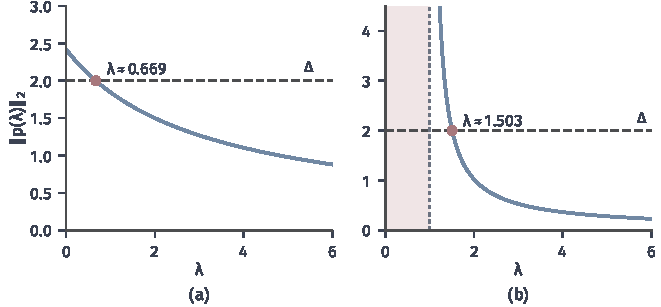
\includegraphics[width=112mm]{figures/05-optimization/02-smooth-optimization/matplotlib/tr-secular/figure.pdf}
 \caption{解的长度$\lVert\bm{p}(\lambda)\rVert_2$（蓝）与半径$\Delta=2$（虚线）的交点（红）给出乘子。(a)~点$\bm{a}$，$\bm{B}$正定，曲线从Newton步的长度开始下降。(b)~原点，$\bm{B}$的最小特征值为$-1$，红色浅底的区域$\lambda<1$不满足$\bm{B}+\lambda\bm{I}\succeq\bm{0}$。}
 \label{fig:tr-secular}
\end{BookInlineFigure}

\paragraph{困难情形}
上面的论证依赖$\langle\bm{q}_1,\bm{g}\rangle\neq0$。如果梯度与最小特征值的特征空间正交，式~\eqref{eq:tr-secular}中对应的项消失，曲线在$\lambda=-\lambda_1$处不再趋于无穷，久期方程可能无解。这称为子问题的\term{困难情形}（hard case）。

看下面这组数据：
\[
 \bm{g}=\begin{bmatrix}0\\1\end{bmatrix},\qquad\bm{B}=\begin{bmatrix}-1&0\\0&3\end{bmatrix},\qquad\Delta=1.
\]

当$\lambda>1$时，第一式给出的解是
\[
 \bm{p}(\lambda)=\begin{bmatrix}0\\-1/(\lambda+3)\end{bmatrix},
\]
长度小于$1/4$，够不到边界。定理~\ref{thm:tr-exact}要求$\lambda\geq1$，所以只能取$\lambda=1$。此时$\bm{B}+\bm{I}=\operatorname{diag}(0,4)$奇异，方程的解不唯一：
\[
 \bm{p}=\begin{bmatrix}\tau\\-1/4\end{bmatrix},\qquad\tau\in\mathbb{R}.
\]

沿奇异方向补足长度，使$\lVert\bm{p}\rVert_2=1$，得到两个全局解：
\[
 \tau=\pm\frac{\sqrt{15}}{4},\qquad m(\bm{p})-m(\bm{0})=-\frac58.
\]
图~\ref{fig:tr-hard-case}比较了$g_1$很小与$g_1=0$两种情形。$g_1=0.1$时交点贴近$\lambda=1$；$g_1$恰好为零时，曲线在$\lambda=1$处停在$1/4$，交点消失，解要靠特征向量补足。

\begin{BookInlineFigure}
 \centering
 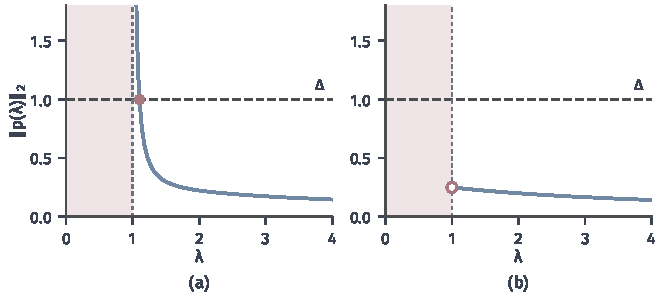
\includegraphics[width=112mm]{figures/05-optimization/02-smooth-optimization/matplotlib/tr-hard-case/figure.pdf}
 \caption{$\bm{B}=\operatorname{diag}(-1,3)$，$\Delta=1$（虚线）时的解长度（蓝）。(a)~$\bm{g}=(0.1,1)^\top$，曲线在$\lambda=1$处趋于无穷，有交点。(b)~$\bm{g}=(0,1)^\top$，曲线只到$1/4$（空心点），与虚线不相交，这是困难情形。}
 \label{fig:tr-hard-case}
\end{BookInlineFigure}

\paragraph{三个不同的量}
子问题的解、模型的下降、真实目标的下降是三件事，下面把它们分开。对候选步$\bm{p}$，定义\term{预测下降}（predicted reduction）和\term{实际下降}（actual reduction）：
\begin{equation}
 \operatorname{pred}(\bm{p})=m(\bm{0})-m(\bm{p}),\qquad
 \operatorname{ared}(\bm{p})=f(\bm{x})-f(\bm{x}+\bm{p}).
 \label{eq:tr-pred-ared}
\end{equation}

子问题的全局解使预测下降最大，却未必使实际下降最大。在原点取$\Delta=2$，全局解是$\bm{p}^\star\approx(-1.988,-0.222)^\top$。由式~\eqref{eq:tr-example-error}，它的模型误差大约是$\tfrac14(1.988)^4\approx3.90$，于是
\[
 \operatorname{pred}(\bm{p}^\star)\approx4.111,\qquad
 \operatorname{ared}(\bm{p}^\star)\approx0.209.
\]

再看同一个球内的另一个点$\bm{p}=(-1.6,-1.2)^\top$。它的预测下降小得多，实际下降反而大一些：
\[
 \operatorname{pred}(\bm{p})=1.92,\qquad
 \operatorname{ared}(\bm{p})\approx0.282.
\]

这个对比说明，模型下降的大小只是在模型的范围内才有意义。图~\ref{fig:tr-three-decreases}画出全局解的两种下降随半径的变化：半径小时两条曲线重合，半径大时预测下降继续上升，实际下降掉头向下。预测和实际的差距正是调整半径的依据，后面第~\ref{sec:tr-acceptance}节用它们的比值组织迭代。

\begin{BookInlineFigure}
 \centering
 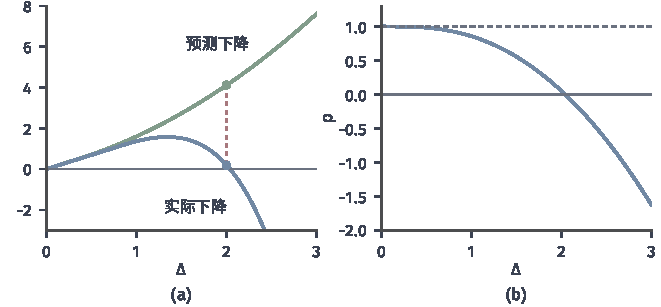
\includegraphics[width=112mm]{figures/05-optimization/02-smooth-optimization/matplotlib/tr-three-decreases/figure.pdf}
 \caption{原点处子问题全局解随半径的变化。(a)~预测下降（绿）与实际下降（蓝），红色虚线标出$\Delta=2$处的差距。(b)~实际下降与预测下降之比$\rho$（蓝），半径越大越偏离$1$，在$\Delta$约为$2$时降到零附近。}
 \label{fig:tr-three-decreases}
\end{BookInlineFigure}

\section{子问题的求解}
\label{sec:tr-subproblem}

第~\ref{sec:tr-model}节的刻画需要分解$\bm{B}+\lambda\bm{I}$好几次，每一轮外层迭代都这样做，代价可能比外层本身还高。接下来要弄清：能否用便宜得多的办法得到一个“够用”的步？

下面对同一个模型和同一个半径比较三种计算。它们是：只沿负梯度取步、把负梯度步与Newton步连起来、用共轭梯度迭代逐步逼近。主例取点$\bm{a}$的数据~\eqref{eq:tr-data-a}，半径$\Delta=2$；Hessian不定的情形用原点的数据~\eqref{eq:tr-data-o}。外层迭代真正需要的，不是子问题的精确解，而是模型下降达到一个规定的比例。这个比例由最简单的那种步来给出。

本节所有量都在同一轮外层迭代内，省略上标$(t)$，写$m,\bm{g},\bm{B},\Delta$。

\subsection{Cauchy步}
\label{sec:tr-cauchy}

\paragraph{沿负梯度最小化模型}
最便宜的做法是只在负梯度这条射线上找模型的最小点。设$\bm{g}\neq\bm{0}$，把点写成$\bm{p}=-a\,\bm{g}/\lVert\bm{g}\rVert_2$，其中$a\in[0,\Delta]$是走过的长度。令
\[
 \kappa=\frac{\bm{g}^\top\bm{B}\bm{g}}{\lVert\bm{g}\rVert_2^2},
\]
它是模型沿负梯度方向的曲率。代入式~\eqref{eq:tr-model}，模型的变化量是一元二次函数
\begin{equation}
 \psi(a)=m\Bigl(-a\frac{\bm{g}}{\lVert\bm{g}\rVert_2}\Bigr)-m(\bm{0})=-a\lVert\bm{g}\rVert_2+\frac{\kappa}{2}a^2.
 \label{eq:tr-cauchy-psi}
\end{equation}

在$[0,\Delta]$上最小化$\psi$，分两种情形。若$\kappa\leq0$，$\psi$严格递减，应当走到边界$a=\Delta$。若$\kappa>0$，$\psi$的顶点在$a=\lVert\bm{g}\rVert_2/\kappa$，它在区间内就取顶点，否则截断在边界。合起来就得到\term{Cauchy步}（Cauchy step）的长度，步本身记为$\bm{p}^{\mathrm{C}}$：
\begin{equation}
 \bm{p}^{\mathrm{C}}=-a^{\mathrm{C}}\frac{\bm{g}}{\lVert\bm{g}\rVert_2},\qquad
 a^{\mathrm{C}}=
 \begin{cases}
  \Delta,&\kappa\leq0,\\
  \min\{\Delta,\ \lVert\bm{g}\rVert_2/\kappa\},&\kappa>0.
 \end{cases}
 \label{eq:tr-cauchy-step}
\end{equation}
图~\ref{fig:tr-cauchy-cases}画出三种情形。计算时只需要一次矩阵向量乘积$\bm{B}\bm{g}$。

\begin{BookInlineFigure}
 \centering
 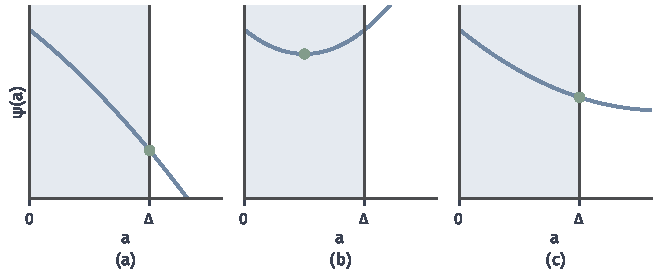
\includegraphics[width=112mm]{figures/05-optimization/02-smooth-optimization/matplotlib/tr-cauchy-cases/figure.pdf}
 \caption{函数$\psi(a)$（蓝）的三种情形，浅蓝带是可取的范围，深灰线是边界，绿点是Cauchy步的长度。(a)~$\kappa\leq0$，走到边界。(b)~$\kappa>0$且顶点在区间内，取顶点。(c)~$\kappa>0$但顶点在区间外，截断在边界。}
 \label{fig:tr-cauchy-cases}
\end{BookInlineFigure}

点$\bm{a}$的数据上，$\bm{g}^\top\bm{B}\bm{g}=49\times14=686$，$\lVert\bm{g}\rVert_2^2=98$，所以
\[
 \kappa=7,\qquad\lVert\bm{g}\rVert_2=7\sqrt2,\qquad\frac{\lVert\bm{g}\rVert_2}{\kappa}=\sqrt2.
\]

半径$\Delta=2$大于$\sqrt2$，Cauchy步取顶点：
\[
 \bm{p}^{\mathrm{C}}=-\sqrt2\cdot\frac{(7,7)^\top}{7\sqrt2}=\begin{bmatrix}-1\\-1\end{bmatrix},\qquad
 \operatorname{pred}(\bm{p}^{\mathrm{C}})=7\sqrt2\cdot\sqrt2-\frac72\cdot2=7.
\]
半径若取$\Delta=1$，则截断在边界，$a^{\mathrm{C}}=1$，预测下降为$7\sqrt2-3.5\approx6.40$。

\paragraph{Cauchy步提供的模型下降}
Cauchy步便宜，它的价值却在于给出了一条有保证的下限。下面的引理说明，它的预测下降由梯度大小、半径和曲率上界控制。

\begin{lemma}[Cauchy步的下降量]
 \label{lem:tr-cauchy-decrease}
 设$\bm{g}\neq\bm{0}$，$\bm{B}$对称。Cauchy步满足
 \begin{equation}
  \operatorname{pred}(\bm{p}^{\mathrm{C}})\geq\frac12\lVert\bm{g}\rVert_2\min\Bigl\{\Delta,\ \frac{\lVert\bm{g}\rVert_2}{\lVert\bm{B}\rVert_2}\Bigr\},
  \label{eq:tr-cauchy-decrease}
 \end{equation}
 其中$\bm{B}=\bm{0}$时第二项理解为$+\infty$。
\end{lemma}

\begin{proof}
 由式~\eqref{eq:tr-cauchy-psi}，预测下降是
 \[
  \operatorname{pred}(\bm{p}^{\mathrm{C}})=a^{\mathrm{C}}\lVert\bm{g}\rVert_2-\frac{\kappa}{2}(a^{\mathrm{C}})^2,
 \]
 并且$\kappa\leq\lVert\bm{B}\rVert_2$。按三种情形估计。

 若$\kappa\leq0$，则$a^{\mathrm{C}}=\Delta$，第二项非负，所以
 \[
  \operatorname{pred}(\bm{p}^{\mathrm{C}})\geq\Delta\lVert\bm{g}\rVert_2.
 \]

 若$\kappa>0$且$\lVert\bm{g}\rVert_2/\kappa\leq\Delta$，则取顶点，所以
 \[
  \operatorname{pred}(\bm{p}^{\mathrm{C}})=\frac{\lVert\bm{g}\rVert_2^2}{2\kappa}\geq\frac{\lVert\bm{g}\rVert_2^2}{2\lVert\bm{B}\rVert_2}.
 \]

 若$\kappa>0$且$\lVert\bm{g}\rVert_2/\kappa>\Delta$，则$a^{\mathrm{C}}=\Delta$，并且$\kappa\Delta<\lVert\bm{g}\rVert_2$，所以
 \[
  \operatorname{pred}(\bm{p}^{\mathrm{C}})=\Delta\lVert\bm{g}\rVert_2-\frac{\kappa\Delta}{2}\Delta\geq\frac12\Delta\lVert\bm{g}\rVert_2.
 \]
 三种情形都不小于式~\eqref{eq:tr-cauchy-decrease}的右端。
\end{proof}

点$\bm{a}$的数据上$\lVert\bm{B}\rVert_2=11$，取$\Delta=2$，式~\eqref{eq:tr-cauchy-decrease}的右端是
\[
 \frac12\cdot7\sqrt2\cdot\min\Bigl\{2,\ \frac{7\sqrt2}{11}\Bigr\}=\frac{49}{11}\approx4.45,
\]
确实不超过实际的预测下降$7$。这个下限比实际值松，它的用处在于对所有模型一致成立。

这条下限只用到一阶信息和曲率的上界，$\bm{B}$可以不定。我们把它提升为对任意候选步的要求：若存在常数$c_1\in(0,1]$，使得
\begin{equation}
 \operatorname{pred}(\bm{p})\geq c_1\lVert\bm{g}\rVert_2\min\Bigl\{\Delta,\ \frac{\lVert\bm{g}\rVert_2}{\lVert\bm{B}\rVert_2}\Bigr\},
 \label{eq:tr-sufficient-decrease}
\end{equation}
就说$\bm{p}$达到\term{充分模型下降}（sufficient model decrease）。第~\ref{sec:tr-convergence}节会看到，一阶收敛只需要这一条；任何预测下降不低于Cauchy步的求解器，都自动满足它，$c_1=1/2$。

要分清这条保障和精确求解的差别。式~\eqref{eq:tr-sufficient-decrease}只是一条下限，并不表示接近子问题的最优值。点$\bm{a}$上Cauchy步的预测下降是$7$，全局解是$10.115$；原点上$\Delta=2$时，Cauchy步是$1$，全局解是$4.111$。只用Cauchy步的方法本质上是最速下降，保留了收敛性，也保留了最速下降的慢。下面两种办法都从它出发，再往前走。

\subsection{狗腿法}
\label{sec:tr-dogleg}

\paragraph{主要思想}
设$\bm{B}\succ\bm{0}$。半径很小时，子问题的解贴近负梯度方向；半径足够大时，解就是Newton点。图~\ref{fig:tr-line-vs-region}中的绿线连接着这两端。求这条曲线要解久期方程，代价较高，\term{狗腿法}（dogleg method）用两段折线代替它。

折线的三个端点是原点、模型沿负梯度的最小点，以及Newton点：
\begin{equation}
 \bm{p}^{\mathrm{U}}=-\frac{\bm{g}^\top\bm{g}}{\bm{g}^\top\bm{B}\bm{g}}\bm{g},\qquad
 \bm{p}^{\mathrm{N}}=-\bm{B}^{-1}\bm{g}.
 \label{eq:tr-dogleg-points}
\end{equation}
上标U表示无约束（unconstrained）。用$\tau\in[0,2]$作路径的参数：
\begin{equation}
 \bm{p}(\tau)=
 \begin{cases}
  \tau\,\bm{p}^{\mathrm{U}},&0\leq\tau\leq1,\\
  \bm{p}^{\mathrm{U}}+(\tau-1)(\bm{p}^{\mathrm{N}}-\bm{p}^{\mathrm{U}}),&1\leq\tau\leq2.
 \end{cases}
 \label{eq:tr-dogleg-path}
\end{equation}

狗腿法在这条路径上走，走到半径为止。这样做合理，要靠路径的两个性质：沿路径越走越远，模型值也越走越低。前者保证路径与球面至多相交一次，后者保证交点是路径上模型最低的可行点。图~\ref{fig:tr-dogleg-monotone}是点$\bm{a}$上的这两条曲线，下面的引理给出证明。

\begin{BookInlineFigure}
 \centering
 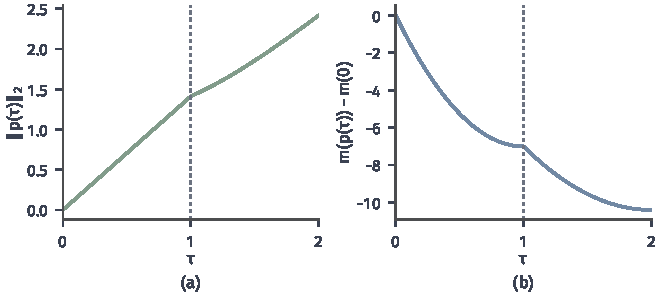
\includegraphics[width=112mm]{figures/05-optimization/02-smooth-optimization/matplotlib/tr-dogleg-monotone/figure.pdf}
 \caption{点$\bm{a}$的数据上沿狗腿路径的两个量，虚线$\tau=1$是折点$\bm{p}^{\mathrm{U}}$。(a)~长度严格增加。(b)~模型值严格减小。}
 \label{fig:tr-dogleg-monotone}
\end{BookInlineFigure}

\begin{lemma}[狗腿路径的单调性]
 \label{lem:tr-dogleg-monotone}
 设$\bm{B}\succ\bm{0}$，$\bm{g}\neq\bm{0}$。沿路径~\eqref{eq:tr-dogleg-path}，$\lVert\bm{p}(\tau)\rVert_2$单调不减，$m(\bm{p}(\tau))$单调不增。
\end{lemma}

\begin{proof}
 第一段上$\bm{p}$是从原点出发的线段，长度递增；$\bm{p}^{\mathrm{U}}$是模型沿这条射线的最小点，模型值递减。

 第二段记$\bm{w}=\bm{p}^{\mathrm{N}}-\bm{p}^{\mathrm{U}}$，$s=\tau-1\in[0,1]$。先看模型值。$h(s)=m(\bm{p}^{\mathrm{U}}+s\bm{w})$是凸二次函数，它在$s=1$处的导数是
 \[
  h'(1)=\langle\bm{B}\bm{p}^{\mathrm{N}}+\bm{g},\bm{w}\rangle=0,
 \]
 因为$\bm{B}\bm{p}^{\mathrm{N}}=-\bm{g}$。凸函数的导数单调不减，所以在$[0,1]$上$h'\leq0$。

 再看长度。$\tfrac12\lVert\bm{p}^{\mathrm{U}}+s\bm{w}\rVert_2^2$对$s$的导数是$\langle\bm{p}^{\mathrm{U}},\bm{w}\rangle+s\lVert\bm{w}\rVert_2^2$，只需证$\langle\bm{p}^{\mathrm{U}},\bm{w}\rangle\geq0$。记$\tau_{\mathrm{U}}>0$为式~\eqref{eq:tr-dogleg-points}中$\bm{g}$前的系数，代入该式，得到
 \[
  \langle\bm{p}^{\mathrm{U}},\bm{w}\rangle=\tau_{\mathrm{U}}\,\bm{g}^\top\bm{B}^{-1}\bm{g}-\tau_{\mathrm{U}}^2\,\bm{g}^\top\bm{g}
  =\frac{\tau_{\mathrm{U}}\bigl[(\bm{g}^\top\bm{B}^{-1}\bm{g})(\bm{g}^\top\bm{B}\bm{g})-(\bm{g}^\top\bm{g})^2\bigr]}{\bm{g}^\top\bm{B}\bm{g}}.
 \]
 取$\bm{u}=\bm{B}^{1/2}\bm{g}$，$\bm{v}=\bm{B}^{-1/2}\bm{g}$，方括号就是$\lVert\bm{u}\rVert_2^2\lVert\bm{v}\rVert_2^2-\langle\bm{u},\bm{v}\rangle^2$，由Cauchy--Schwarz不等式非负。
\end{proof}

\paragraph{计算过程}
下面用点$\bm{a}$的数据~\eqref{eq:tr-data-a}、半径$\Delta=2$走一遍。

需要的量是梯度$\bm{g}\in\mathbb{R}^n$、对称正定矩阵$\bm{B}\in\mathbb{R}^{n\times n}$、半径$\Delta$，输出位移$\bm{p}$。例中已知$\bm{g}=(7,7)^\top$，$\bm{B}=\operatorname{diag}(11,3)$。步骤如下。

\begin{enumerate}
 \item 由式~\eqref{eq:tr-dogleg-points}计算Newton点，若$\lVert\bm{p}^{\mathrm{N}}\rVert_2\leq\Delta$，返回$\bm{p}=\bm{p}^{\mathrm{N}}$。例中
 \[
  \bm{p}^{\mathrm{N}}=\begin{bmatrix}-7/11\\-7/3\end{bmatrix},\qquad\lVert\bm{p}^{\mathrm{N}}\rVert_2\approx2.419>2,
 \]
 所以继续。
 \item 由式~\eqref{eq:tr-dogleg-points}计算$\bm{p}^{\mathrm{U}}$，若$\lVert\bm{p}^{\mathrm{U}}\rVert_2\geq\Delta$，返回边界上的负梯度步$\bm{p}=-\Delta\bm{g}/\lVert\bm{g}\rVert_2$，这就是Cauchy步。例中
 \[
  \bm{p}^{\mathrm{U}}=-\frac{98}{686}\begin{bmatrix}7\\7\end{bmatrix}=\begin{bmatrix}-1\\-1\end{bmatrix},\qquad\lVert\bm{p}^{\mathrm{U}}\rVert_2=\sqrt2<2,
 \]
 所以继续。
 \item 否则交点在第二段上。记$\bm{w}=\bm{p}^{\mathrm{N}}-\bm{p}^{\mathrm{U}}$，解$\lVert\bm{p}^{\mathrm{U}}+s\bm{w}\rVert_2=\Delta$的正根：
 \begin{equation}
  s=\frac{-\langle\bm{p}^{\mathrm{U}},\bm{w}\rangle+\sqrt{\langle\bm{p}^{\mathrm{U}},\bm{w}\rangle^2+\lVert\bm{w}\rVert_2^2\bigl(\Delta^2-\lVert\bm{p}^{\mathrm{U}}\rVert_2^2\bigr)}}{\lVert\bm{w}\rVert_2^2}.
  \label{eq:tr-boundary-root}
 \end{equation}
 例中$\bm{w}=(4/11,\,-4/3)^\top$，三个系数是
 \[
  \lVert\bm{w}\rVert_2^2=\frac{2080}{1089},\qquad\langle\bm{p}^{\mathrm{U}},\bm{w}\rangle=\frac{1056}{1089},\qquad\Delta^2-\lVert\bm{p}^{\mathrm{U}}\rVert_2^2=2.
 \]
 根号内的量是$(2376/1089)^2$，因此
 \[
  s=\frac{-1056+2376}{2080}=\frac{33}{52}.
 \]
 \item 返回$\bm{p}=\bm{p}^{\mathrm{U}}+s\bm{w}$。例中
 \[
  \bm{p}=\begin{bmatrix}-1+3/13\\-1-11/13\end{bmatrix}=\begin{bmatrix}-10/13\\-24/13\end{bmatrix},
 \]
 长度恰为$\sqrt{100+576}/13=2$。
\end{enumerate}

最终得到的预测下降是
\[
 \operatorname{pred}(\bm{p})=\frac{238}{13}-\frac{1414}{169}=\frac{1680}{169}\approx9.941.
\]
这已经是全局解$10.115$的$98\%$，而全局解要解一元非线性方程。图~\ref{fig:tr-dogleg-path}给出三种半径下的结果：$\Delta=1$时只用到第一段，$\Delta=2$时落在第二段，$\Delta=3$时完整的Newton步被采用。

\begin{BookInlineFigure}
 \centering
 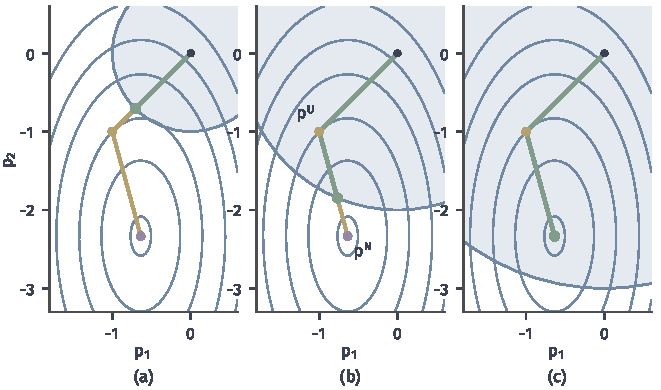
\includegraphics[width=112mm]{figures/05-optimization/02-smooth-optimization/matplotlib/tr-dogleg-path/figure.pdf}
 \caption{点$\bm{a}$的数据上半径分别为$1$、$2$、$3$的狗腿步。黄线是完整路径，绿线是实际走过的部分，绿点是得到的步。黄点是$\bm{p}^{\mathrm{U}}$，紫点是$\bm{p}^{\mathrm{N}}$，蓝线是模型等高线，浅蓝圆盘是信赖域。}
 \label{fig:tr-dogleg-path}
\end{BookInlineFigure}

狗腿步的预测下降不低于Cauchy步：若$\lVert\bm{p}^{\mathrm{U}}\rVert_2\geq\Delta$，两者相同；否则$\bm{p}^{\mathrm{U}}$本身就是Cauchy步，而由引理~\ref{lem:tr-dogleg-monotone}，狗腿步在路径上更靠后，模型值更低。所以它满足式~\eqref{eq:tr-sufficient-decrease}，$c_1=1/2$。

\paragraph{不正定时不能照搬}
上面的构造用到$\bm{B}\succ\bm{0}$：$\bm{p}^{\mathrm{N}}$要是模型的最小点，第二段上的模型才会下降。把原点的数据~\eqref{eq:tr-data-o}照搬进去，$\bm{g}^\top\bm{B}\bm{g}=2>0$，第一段还能算出$\bm{p}^{\mathrm{U}}=(-1,-1)^\top$，第二段却指向鞍点$(1,-1/3)^\top$。沿第二段模型上升，从$-1$一直升到$1/3$，图~\ref{fig:tr-dogleg-indefinite}画出了这一段。

\begin{BookInlineFigure}
 \centering
 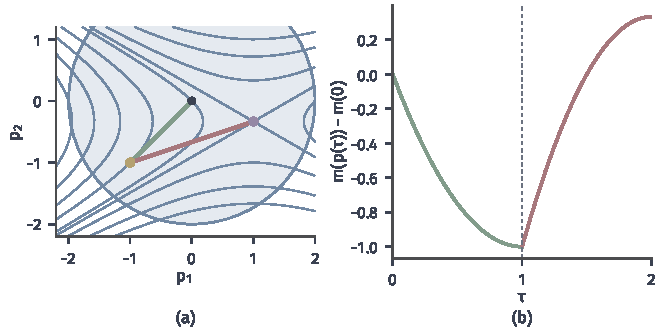
\includegraphics[width=112mm]{figures/05-optimization/02-smooth-optimization/matplotlib/tr-dogleg-indefinite/figure.pdf}
 \caption{把狗腿路径照搬到原点的不定模型上。(a)~模型等高线（蓝）与路径：绿色第一段走向黄点$\bm{p}^{\mathrm{U}}$，红色第二段走向模型的鞍点（紫）。(b)~沿路径的模型值，第二段（红）上升，路径上模型值的单调性失效。}
 \label{fig:tr-dogleg-indefinite}
\end{BookInlineFigure}

$\bm{B}$半正定且奇异时，$\bm{B}^{-1}$不存在，构造同样失效。这时要么先把$\bm{B}$修正成正定，要么换用下一小节的方法，后者不需要$\bm{B}$的任何分解。

\subsection{截断共轭梯度}
\label{sec:tr-truncated-cg}

\paragraph{主要思想}
Newton步是方程$\bm{B}\bm{p}=-\bm{g}$的解，也就是模型的驻点。第~\ref{chap:second-order-methods}章的Newton-CG用共轭梯度迭代近似解这个方程，只需要矩阵向量乘积。共轭梯度的推导和收敛性质可参考\BookChapterRef{chap:krylov-methods}{卷二第15章“Krylov子空间法”}，这里复述要用到的部分。

从$\bm{p}^{(0)}=\bm{0}$出发，记残差$\bm{r}^{(j)}=\bm{B}\bm{p}^{(j)}+\bm{g}$，它恰好是模型在$\bm{p}^{(j)}$处的梯度。内层迭代的上标用$j$，与外层的$t$区分。共轭梯度的递推是
\begin{equation}
 \begin{gathered}
  \alpha^{(j)}=\frac{\lVert\bm{r}^{(j)}\rVert_2^2}{\bm{d}^{(j)\top}\bm{B}\bm{d}^{(j)}},\qquad
  \bm{p}^{(j+1)}=\bm{p}^{(j)}+\alpha^{(j)}\bm{d}^{(j)},\\
  \bm{r}^{(j+1)}=\bm{r}^{(j)}+\alpha^{(j)}\bm{B}\bm{d}^{(j)},\\
  \beta^{(j)}=\frac{\lVert\bm{r}^{(j+1)}\rVert_2^2}{\lVert\bm{r}^{(j)}\rVert_2^2},\qquad
  \bm{d}^{(j+1)}=-\bm{r}^{(j+1)}+\beta^{(j)}\bm{d}^{(j)},
 \end{gathered}
 \label{eq:tr-cg}
\end{equation}
初始方向$\bm{d}^{(0)}=-\bm{g}$。$\alpha^{(j)}$是模型沿$\bm{d}^{(j)}$的精确一维最小点，所以每步模型值都下降。第一步恰好是$\bm{p}^{\mathrm{U}}$。

放进信赖域，只需要回答两个新问题：迭代走出半径了怎么办，遇到$\bm{B}$的非正曲率怎么办。\term{截断共轭梯度法}（truncated conjugate gradient method）的回答是：两种情况都沿当前方向走到边界，然后停止。

先看走出半径的情形。下面的引理说明，共轭梯度的迭代点离原点越来越远。一旦越出球，以后就不会回来，所以在第一次越界处截断不会错过后面的点。

\begin{lemma}[迭代点的长度递增]
 \label{lem:tr-cg-norm}
 设$\bm{g}\neq\bm{0}$，递推~\eqref{eq:tr-cg}进行到第$j$步，且此前各步曲率$\bm{d}^{(i)\top}\bm{B}\bm{d}^{(i)}>0$，残差非零。则
 \begin{equation}
  \lVert\bm{p}^{(j+1)}\rVert_2>\lVert\bm{p}^{(j)}\rVert_2.
  \label{eq:tr-cg-norm}
 \end{equation}
\end{lemma}

\begin{proof}
 残差相互正交，并且方向与残差张成同一子空间：
 \[
  \operatorname{span}\{\bm{d}^{(0)},\ldots,\bm{d}^{(j-1)}\}=\operatorname{span}\{\bm{r}^{(0)},\ldots,\bm{r}^{(j-1)}\}.
 \]
 这两条性质的归纳证明只用到递推~\eqref{eq:tr-cg}中的分母非零，不要求$\bm{B}$在全空间正定。由于$\bm{p}^{(j)}$是$\bm{d}^{(0)},\ldots,\bm{d}^{(j-1)}$的线性组合，所以$\langle\bm{p}^{(j)},\bm{r}^{(j)}\rangle=0$。

 用归纳法证明$\langle\bm{p}^{(j)},\bm{d}^{(j)}\rangle\geq0$。$j=0$时等于$0$。代入$\bm{d}^{(j+1)}$的定义，并用正交性，得到
 \[
  \langle\bm{p}^{(j+1)},\bm{d}^{(j+1)}\rangle=\beta^{(j)}\langle\bm{p}^{(j+1)},\bm{d}^{(j)}\rangle
  =\beta^{(j)}\bigl(\langle\bm{p}^{(j)},\bm{d}^{(j)}\rangle+\alpha^{(j)}\lVert\bm{d}^{(j)}\rVert_2^2\bigr),
 \]
 其中$\alpha^{(j)},\beta^{(j)}>0$，因此它非负。

 最后展开长度：
 \[
  \lVert\bm{p}^{(j+1)}\rVert_2^2=\lVert\bm{p}^{(j)}\rVert_2^2+2\alpha^{(j)}\langle\bm{p}^{(j)},\bm{d}^{(j)}\rangle+(\alpha^{(j)})^2\lVert\bm{d}^{(j)}\rVert_2^2>\lVert\bm{p}^{(j)}\rVert_2^2.
 \]
\end{proof}

再看非正曲率的情形。若$\bm{d}^{(j)\top}\bm{B}\bm{d}^{(j)}\leq0$，模型沿$\bm{d}^{(j)}$是凹的。由$\bm{r}^{(j)}$与$\bm{d}^{(j-1)}$正交可知模型沿$\bm{d}^{(j)}$的斜率为$-\lVert\bm{r}^{(j)}\rVert_2^2<0$，所以越往前走模型越低，应当一直走到边界。这正是第~\ref{sec:tr-model}节所说的利用负曲率。

三种停止各有含义，图~\ref{fig:tr-tcg-flow}是一步迭代的判断顺序。残差停止表示模型的驻点已经解得够准，判据沿用第~\ref{chap:second-order-methods}章非精确Newton法的形式：
\begin{equation}
 \lVert\bm{r}^{(j)}\rVert_2\leq\eta\lVert\bm{g}\rVert_2,\qquad\eta=\min\{0.1,\ \sqrt{\lVert\bm{g}\rVert_2}\}.
 \label{eq:tr-residual-stop}
\end{equation}

边界停止表示模型的最小点在球外。曲率停止表示模型沿这个方向没有最小点。后两条是信赖域给内层迭代新加的规则，Newton-CG遇到非正曲率时只能退回一个下降方向，交给线搜索。

\begin{BookInlineFigure}
 \centering
 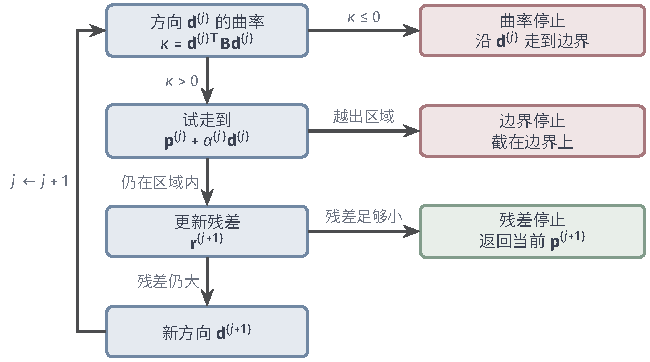
\includegraphics[width=110mm]{figures/05-optimization/02-smooth-optimization/tikz/tr-tcg-flow/figure.pdf}
 \caption{截断共轭梯度一次内层迭代的判断顺序。蓝框是普通的共轭梯度步骤，红框是信赖域带来的两种截断，绿框是沿用Newton-CG的残差停止。}
 \label{fig:tr-tcg-flow}
\end{BookInlineFigure}

\needspace{6\baselineskip}
\paragraph{变量}
下面的过程结合点$\bm{a}$的数据走一遍，要维护的量是：
\begin{itemize}
 \item $\bm{p}^{(j)}\in\mathbb{R}^n$：当前位移；
 \item $\bm{r}^{(j)}\in\mathbb{R}^n$：模型在$\bm{p}^{(j)}$处的梯度；
 \item $\bm{d}^{(j)}\in\mathbb{R}^n$：搜索方向；
 \item $\bm{B}\bm{d}^{(j)}\in\mathbb{R}^n$：一次矩阵向量乘积，是全部需要的曲率信息。
\end{itemize}

\paragraph{初始化}
取$\bm{p}^{(0)}=\bm{0}$，$\bm{r}^{(0)}=\bm{g}$，$\bm{d}^{(0)}=-\bm{g}$，容差$\eta$。例中半径$\Delta=2$，容差取$\eta=0.1$：
\[
 \bm{r}^{(0)}=\begin{bmatrix}7\\7\end{bmatrix},\qquad
 \bm{d}^{(0)}=\begin{bmatrix}-7\\-7\end{bmatrix},\qquad
 \eta\lVert\bm{g}\rVert_2\approx0.990.
\]

\paragraph{每轮更新}
第$j$轮依次执行以下步骤。

\begin{enumerate}
 \item 计算$\bm{B}\bm{d}^{(j)}$和曲率$\bm{d}^{(j)\top}\bm{B}\bm{d}^{(j)}$。若曲率不大于零，按式~\eqref{eq:tr-boundary-root}（其中$\bm{p}^{\mathrm{U}}$换成$\bm{p}^{(j)}$，$\bm{w}$换成$\bm{d}^{(j)}$）求出边界上的$\sigma$，返回$\bm{p}^{(j)}+\sigma\bm{d}^{(j)}$。例中第一轮
 \[
  \bm{B}\bm{d}^{(0)}=\begin{bmatrix}-77\\-21\end{bmatrix},\qquad
  \bm{d}^{(0)\top}\bm{B}\bm{d}^{(0)}=686>0.
 \]
 \item 由式~\eqref{eq:tr-cg}计算$\alpha^{(j)}$和试探点$\bm{p}^{(j)}+\alpha^{(j)}\bm{d}^{(j)}$。若试探点的长度不小于$\Delta$，同样求边界上的$\sigma$并返回。例中第一轮
 \[
  \alpha^{(0)}=\frac{98}{686}=\frac17,\qquad
  \bm{p}^{(1)}=\begin{bmatrix}-1\\-1\end{bmatrix},\qquad\lVert\bm{p}^{(1)}\rVert_2=\sqrt2<2.
 \]
 \item 由式~\eqref{eq:tr-cg}更新残差，若$\bm{r}^{(j+1)}$满足式~\eqref{eq:tr-residual-stop}，返回$\bm{p}^{(j+1)}$。例中第一轮
 \[
  \bm{r}^{(1)}=\begin{bmatrix}7\\7\end{bmatrix}+\frac17\begin{bmatrix}-77\\-21\end{bmatrix}=\begin{bmatrix}-4\\4\end{bmatrix},\qquad
  \lVert\bm{r}^{(1)}\rVert_2\approx5.66>0.990.
 \]
 \item 由式~\eqref{eq:tr-cg}计算$\beta^{(j)}$和新方向。例中第一轮
 \[
  \beta^{(0)}=\frac{32}{98}=\frac{16}{49},\qquad
  \bm{d}^{(1)}=\begin{bmatrix}4\\-4\end{bmatrix}+\frac{16}{49}\begin{bmatrix}-7\\-7\end{bmatrix}=\begin{bmatrix}12/7\\-44/7\end{bmatrix}.
 \]
\end{enumerate}

例中第二轮的曲率是
\[
 \bm{B}\bm{d}^{(1)}=\begin{bmatrix}132/7\\-132/7\end{bmatrix},\qquad
 \bm{d}^{(1)\top}\bm{B}\bm{d}^{(1)}=\frac{7392}{49}>0.
\]

于是$\alpha^{(1)}=32\cdot49/7392=7/33$。试探点正是Newton点，而它的长度约为$2.419$，超过了半径：
\[
 \bm{p}^{(1)}+\alpha^{(1)}\bm{d}^{(1)}=\begin{bmatrix}-7/11\\-7/3\end{bmatrix}.
\]

所以按边界停止。由式~\eqref{eq:tr-boundary-root}，边界上的$\sigma=7/52$，最终得到
\[
 \bm{p}=\begin{bmatrix}-1\\-1\end{bmatrix}+\frac{7}{52}\begin{bmatrix}12/7\\-44/7\end{bmatrix}=\begin{bmatrix}-10/13\\-24/13\end{bmatrix}.
\]

这和狗腿步完全相同，并不是巧合。二维时共轭梯度第一步到$\bm{p}^{\mathrm{U}}$，第二步到$\bm{p}^{\mathrm{N}}$，两段路径就是狗腿路径。维数大于$2$时两者不同：狗腿法从$\bm{p}^{\mathrm{U}}$直奔Newton点，截断共轭梯度沿途经过一串中间点，也不需要预先分解$\bm{B}$。半径若取$\Delta=3$，第二轮的试探点在球内，残差恰好为零，按残差停止，返回Newton步。

再用原点的数据~\eqref{eq:tr-data-o}、$\Delta=2$看曲率停止。第一轮的曲率$\bm{d}^{(0)\top}\bm{B}\bm{d}^{(0)}=2>0$，$\alpha^{(0)}=1$，试探点在球内，并有
\[
 \bm{p}^{(1)}=\begin{bmatrix}-1\\-1\end{bmatrix},\qquad
 \bm{r}^{(1)}=\begin{bmatrix}2\\-2\end{bmatrix},\qquad
 \bm{d}^{(1)}=\begin{bmatrix}-6\\-2\end{bmatrix}.
\]

第二轮的曲率是$-36+12=-24\leq0$，沿$\bm{d}^{(1)}$走到边界。由$\lVert\bm{p}^{(1)}+\sigma\bm{d}^{(1)}\rVert_2=2$得$20\sigma^2+8\sigma-1=0$，取正根$\sigma=1/10$，最终得到
\[
 \bm{p}=\begin{bmatrix}-8/5\\-6/5\end{bmatrix},\qquad\operatorname{pred}(\bm{p})=\frac{48}{25}=1.92.
\]
图~\ref{fig:tr-tcg-path}是这两次运行的轨迹。

\begin{BookInlineFigure}
 \centering
 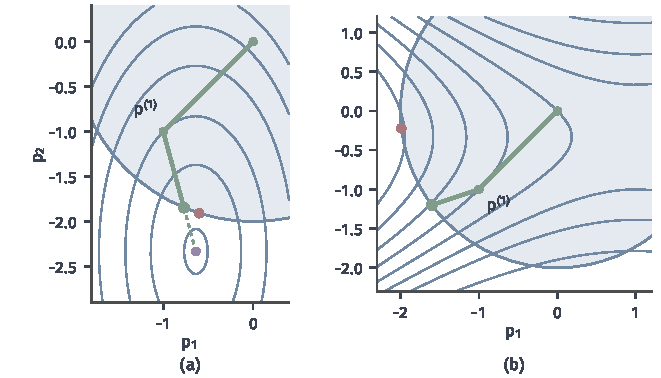
\includegraphics[width=112mm]{figures/05-optimization/02-smooth-optimization/matplotlib/tr-tcg-path/figure.pdf}
 \caption{截断共轭梯度的两次运行，绿线是迭代轨迹，绿色大点是返回的步，红点是子问题的全局解。(a)~点$\bm{a}$，第二轮越过边界而截断，虚线通向球外的Newton点（紫）。(b)~原点，第二轮遇到负曲率，沿方向走到边界。}
 \label{fig:tr-tcg-path}
\end{BookInlineFigure}

\paragraph{算法分析}
截断共轭梯度的第一轮要么到达$\bm{p}^{\mathrm{U}}$，要么在边界上截断，得到的都是Cauchy步，此后每一步模型值都不升高：普通步是精确一维最小化，边界截断发生在模型仍然下降的路段上。所以它的预测下降不低于Cauchy步，满足式~\eqref{eq:tr-sufficient-decrease}，$c_1=1/2$。

当$\bm{B}\succ\bm{0}$时还可以证明，截断共轭梯度的预测下降至少是全局解的一半，证明需要细致比较Krylov子空间上的子问题，篇幅较长，读者可查阅专门的信赖域文献。$\bm{B}$不定时没有这个保证：原点上它的预测下降只有$1.92$，全局解是$4.111$。它在图~\ref{fig:tr-tcg-path}(b)中沿方向$(-3,-1)^\top$走到边界，错过了曲率最负的方向$\bm{e}_1$。

表~\ref{tab:tr-subproblem-compare}汇总同一个模型上三种步和全局解的结果。

\begin{BookInlineTable}
 \centering
 \begin{tabular}{llrrrr}
  \toprule
  模型 & 量 & Cauchy步 & 狗腿步 & 截断共轭梯度 & 全局解\\
  \midrule
  点$\bm{a}$ & $\operatorname{pred}$ & $7.000$ & $9.941$ & $9.941$ & $10.115$\\
  & $\operatorname{ared}$ & $8.750$ & $10.764$ & $10.764$ & $10.515$\\
  原点 & $\operatorname{pred}$ & $1.000$ & 不适用 & $1.920$ & $4.111$\\
  & $\operatorname{ared}$ & $0.750$ & 不适用 & $0.282$ & $0.209$\\
  \bottomrule
 \end{tabular}
 \caption{半径$\Delta=2$时几种步的预测下降与实际下降。}
 \label{tab:tr-subproblem-compare}
\end{BookInlineTable}

二维例子看不出截断共轭梯度的省力之处。图~\ref{fig:tr-tcg-compare}取一个$n=200$的正定模型：Hessian向量乘积只用$9$次，预测下降就达到全局解的$98\%$，长度随次数严格增加，与引理~\ref{lem:tr-cg-norm}一致。这时狗腿法和精确求解都要作$200$阶矩阵的分解。

\begin{BookInlineFigure}
 \centering
 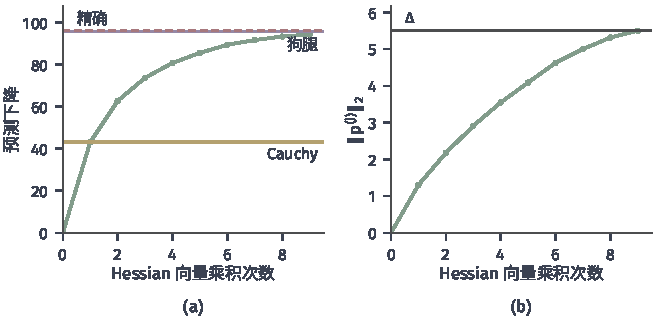
\includegraphics[width=112mm]{figures/05-optimization/02-smooth-optimization/matplotlib/tr-tcg-compare/figure.pdf}
 \caption{一个$n=200$的随机正定模型，特征值在$1$到$100$之间对数等距，$\Delta=5.5$，随机种子固定。(a)~截断共轭梯度（绿）的预测下降随矩阵向量乘积次数的变化，水平线依次为Cauchy步（黄）、狗腿步（紫）和全局解（红虚线）。(b)~迭代点长度（绿）递增，触及半径（深灰线）时停止。}
 \label{fig:tr-tcg-compare}
\end{BookInlineFigure}

\section{步的接受与半径更新}
\label{sec:tr-acceptance}

子问题给出了一个候选步，但模型的话不能全信。这就需要回答：怎样用真实目标检验这一步，并决定下一轮用多大的半径？

\paragraph{主要思想}
第~\ref{sec:tr-model}节已经分开了预测下降和实际下降，把它们相除就是一个无量纲的检验量。定义\term{下降比}（reduction ratio）：
\begin{equation}
 \rho^{(t)}=\frac{\operatorname{ared}(\bm{p}^{(t)})}{\operatorname{pred}(\bm{p}^{(t)})}
 =\frac{f(\bm{x}^{(t)})-f(\bm{x}^{(t)}+\bm{p}^{(t)})}{m^{(t)}(\bm{0})-m^{(t)}(\bm{p}^{(t)})}.
 \label{eq:tr-rho}
\end{equation}
只要$\bm{g}^{(t)}\neq\bm{0}$且候选步满足式~\eqref{eq:tr-sufficient-decrease}，分母就为正，比值有意义。

$\rho^{(t)}$接近$1$，说明模型在这个范围内预测得准。$\rho^{(t)}$是很小的正数，说明目标虽有下降，但比预测差得多。$\rho^{(t)}$为负，说明目标实际上升了。$\rho^{(t)}$大于$1$，说明目标比模型预测的下降更多，这是好事，但也表明模型并不精确。

用两个阈值$0<\eta_1\leq\eta_2<1$把数轴分成三段，常取$\eta_1=1/4$，$\eta_2=3/4$；另取缩小因子$\theta\in(0,1)$和半径上限$\Delta_{\max}$。下一个点按是否接受决定：
\begin{equation}
 \bm{x}^{(t+1)}=
 \begin{cases}
  \bm{x}^{(t)}+\bm{p}^{(t)},&\rho^{(t)}\geq\eta_1,\\
  \bm{x}^{(t)},&\rho^{(t)}<\eta_1.
 \end{cases}
 \label{eq:tr-accept}
\end{equation}

下一轮的半径按模型的表现决定：
\begin{equation}
 \Delta^{(t+1)}=
 \begin{cases}
  \theta\Delta^{(t)},&\rho^{(t)}<\eta_1,\\
  \min\{2\Delta^{(t)},\Delta_{\max}\},&\rho^{(t)}\geq\eta_2\text{ 且步在边界},\\
  \Delta^{(t)},&\text{其他情形}.
 \end{cases}
 \label{eq:tr-radius}
\end{equation}

第二种情形多了“步在边界”这个条件，即$\lVert\bm{p}^{(t)}\rVert_2=\Delta^{(t)}$：若步在球内部，半径并没有限制住它，扩大半径没有意义。图~\ref{fig:tr-rho-decision}把这三段画在数轴上。

\begin{BookInlineFigure}
 \centering
 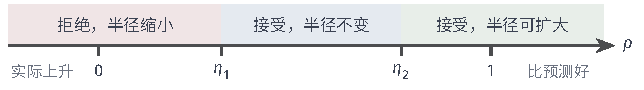
\includegraphics[width=109mm]{figures/05-optimization/02-smooth-optimization/tikz/tr-rho-decision/figure.pdf}
 \caption{下降比$\rho$的三段及相应动作。红色段拒绝这一步，蓝色段接受但半径不变，绿色段接受，并且在步到达边界时扩大半径。}
 \label{fig:tr-rho-decision}
\end{BookInlineFigure}

拒绝一步的代价比看上去小。点没有动，梯度和$\bm{B}$都不用重算，下一轮用同一个模型在更小的球里重解子问题。这里要与线搜索的回溯对比：回溯只缩短长度，方向不变；信赖域缩小半径后，新的解方向一般也变了。图~\ref{fig:tr-loop}是完整的一轮。

\begin{BookInlineFigure}
 \centering
 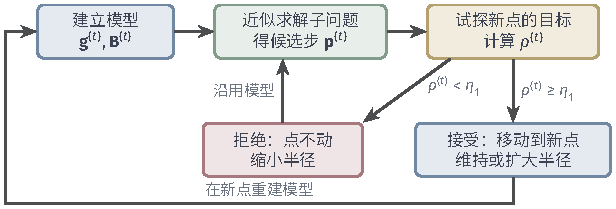
\includegraphics[width=104mm]{figures/05-optimization/02-smooth-optimization/tikz/tr-loop/figure.pdf}
 \caption{信赖域方法的一轮。黄框里的目标值是这一轮唯一一次新增的函数值计算。接受时回到左侧在新点重建模型，拒绝时模型沿用，只在更小的球内重解子问题。}
 \label{fig:tr-loop}
\end{BookInlineFigure}

\paragraph{模型矩阵从哪里来}
框架对$\bm{B}^{(t)}$的要求很少：对称，范数有界。取Hessian得到信赖域Newton法；取第~\ref{chap:quasi-newton}章的BFGS近似也可以。第~\ref{chap:quasi-newton}章的SR1更新尤其适合这里，它由位移$\bm{s}=\bm{p}^{(t)}$和梯度差$\bm{y}$得到
\begin{equation}
 \bm{B}^{(t+1)}=\bm{B}^{(t)}+\frac{(\bm{y}-\bm{B}^{(t)}\bm{s})(\bm{y}-\bm{B}^{(t)}\bm{s})^\top}{\langle\bm{y}-\bm{B}^{(t)}\bm{s},\bm{s}\rangle}.
 \label{eq:tr-sr1}
\end{equation}

SR1不保持正定性，$\bm{B}^{(t+1)}$可能不定，放进线搜索框架时方向可能不是下降方向，这在信赖域中不成问题。分母过小时跳过更新。即使这一步被拒绝，$\bm{s}$和$\bm{y}$仍然是真实的曲率信息，通常也用来更新，代价是在试探点多算一次梯度。这时$\bm{B}^{(t)}$已不是$\bm{H}^{(t)}$，下面的手算例子仍用Hessian。

\needspace{6\baselineskip}
\paragraph{变量}
下面用目标~\eqref{eq:tr-example}走完整个过程，子问题用截断共轭梯度求解。要维护的量是：
\begin{itemize}
 \item $\bm{x}^{(t)}\in\mathbb{R}^n$：当前点，$f(\bm{x}^{(t)})$是它的目标值；
 \item $\Delta^{(t)}>0$：当前半径；
 \item $\bm{g}^{(t)}\in\mathbb{R}^n$，$\bm{B}^{(t)}\in\mathbb{R}^{n\times n}$：当前模型，上一轮被拒绝时直接沿用。
\end{itemize}

\paragraph{初始化}
选定$\bm{x}^{(0)}$，$\Delta^{(0)}$，阈值和缩小因子。例中取
\[
 \bm{x}^{(0)}=\begin{bmatrix}0\\0\end{bmatrix},\qquad\Delta^{(0)}=2,\qquad\Delta_{\max}=8,
\]
\[
 \eta_1=\frac14,\qquad\eta_2=\frac34,\qquad\theta=\frac12.
\]

\paragraph{每轮更新}
第$t$轮依次执行以下步骤，直到$\lVert\bm{g}^{(t)}\rVert_2$小于给定的容差。

\begin{enumerate}
 \item 若上一轮接受了步，由式~\eqref{eq:tr-example-derivatives}计算$\bm{g}^{(t)}$和$\bm{B}^{(t)}$。例中第$0$轮得到数据~\eqref{eq:tr-data-o}。
 \item 近似求解子问题~\eqref{eq:tr-subproblem}，得到$\bm{p}^{(t)}$。例中第$0$轮就是上一节算过的曲率停止：
 \[
  \bm{p}^{(0)}=\begin{bmatrix}-1.6\\-1.2\end{bmatrix},\qquad\operatorname{pred}(\bm{p}^{(0)})=1.92.
 \]
 \item 由式~\eqref{eq:tr-rho}计算$\rho^{(t)}$。例中第$0$轮由式~\eqref{eq:tr-example-error}，模型误差是$\tfrac14(1.6)^4=1.6384$，于是
 \[
  \operatorname{ared}(\bm{p}^{(0)})=1.92-1.6384=0.2816,\qquad\rho^{(0)}\approx0.147.
 \]
 \item 由式~\eqref{eq:tr-accept}和式~\eqref{eq:tr-radius}决定下一个点和半径。例中第$0$轮$\rho^{(0)}<1/4$，拒绝这一步，并有
 \[
  \bm{x}^{(1)}=\begin{bmatrix}0\\0\end{bmatrix},\qquad\Delta^{(1)}=1.
 \]
\end{enumerate}

第$1$轮沿用同一个模型。半径变成$1$，共轭梯度的第一步$(-1,-1)^\top$长度为$\sqrt2$，已越过边界，所以截断在球面上：
\[
 \bm{p}^{(1)}=\begin{bmatrix}-1/\sqrt2\\-1/\sqrt2\end{bmatrix},\qquad\operatorname{pred}(\bm{p}^{(1)})=\sqrt2-\frac12\approx0.9142.
\]

模型误差是$\tfrac14(1/\sqrt2)^4=0.0625$，于是实际下降约为$0.8517$，比值$\rho^{(1)}\approx0.932\geq3/4$。这一步在边界上，接受并把半径扩大：
\[
 \bm{x}^{(2)}\approx\begin{bmatrix}-0.7071\\-0.7071\end{bmatrix},\qquad\Delta^{(2)}=2.
\]
半径减半之后，步的方向由$(-1.6,-1.2)$变成了负梯度方向，这正是前面说的方向随半径变化。图~\ref{fig:tr-rejection}把这两次试探画在真实目标上。

\begin{BookInlineFigure}
 \centering
 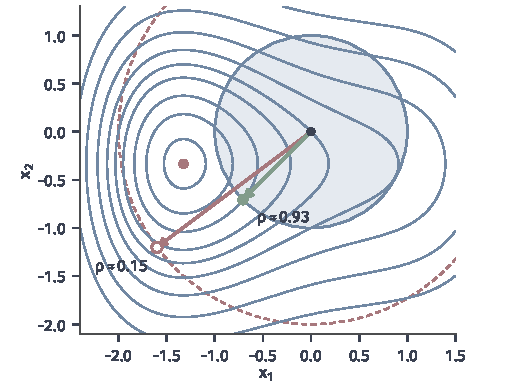
\includegraphics[width=90mm]{figures/05-optimization/02-smooth-optimization/matplotlib/tr-rejection/figure.pdf}
 \caption{原点处的一次拒绝与一次接受，蓝线是目标~\eqref{eq:tr-example}的等高线。红色虚线圆和红色箭头是$\Delta=2$的试探，空心点被拒绝；浅蓝圆盘和绿色箭头是$\Delta=1$的试探，绿点被接受。红色实心点是最小点。}
 \label{fig:tr-rejection}
\end{BookInlineFigure}

第$2$轮由式~\eqref{eq:tr-example-derivatives}重建模型：
\[
 \bm{g}^{(2)}\approx\begin{bmatrix}1.3536\\-1.1213\end{bmatrix},\qquad\bm{B}^{(2)}\approx\begin{bmatrix}0.5&0\\0&3\end{bmatrix}.
\]

这时$\bm{B}$已经正定，但$x_1$方向的曲率只有$0.5$，比前方实际的曲率小得多。$\Delta=2$的步是$\bm{p}^{(2)}\approx(-1.928,0.530)^\top$，预测下降$1.853$，实际却上升$6.674$，$\rho^{(2)}\approx-3.60$，又被拒绝。第$3$轮半径减半后，比值回到$0.589$，接受，半径保持为$1$。

继续下去，第$4$轮开始Newton步已落在球内，由残差停止，半径不再起作用，比值接近$1$，梯度范数迅速下降。表~\ref{tab:tr-history}列出全部$8$轮，最终得到$\bm{x}\approx(-1.3247,-0.3333)^\top$，$f\approx-1.5989$，这就是$\bm{x}^\star$。图~\ref{fig:tr-outer-path}是轨迹和半径的变化。

\begin{BookInlineTable}
 \centering
 \begin{tabular}{rrrcrrrl}
  \toprule
  $t$ & $f(\bm{x}^{(t)})$ & $\Delta^{(t)}$ & 停止 & pred & ared & $\rho^{(t)}$ & 结果\\
  \midrule
  $0$ & $0.000$ & $2$ & 曲率 & $1.920$ & $0.282$ & $0.147$ & 拒绝\\
  $1$ & $0.000$ & $1$ & 边界 & $0.914$ & $0.852$ & $0.932$ & 接受，扩大\\
  $2$ & $-0.852$ & $2$ & 边界 & $1.853$ & $-6.674$ & $-3.602$ & 拒绝\\
  $3$ & $-0.852$ & $1$ & 边界 & $0.999$ & $0.588$ & $0.589$ & 接受\\
  $4$ & $-1.440$ & $1$ & 残差 & $0.155$ & $0.158$ & $1.023$ & 接受\\
  $5$ & $-1.598$ & $1$ & 残差 & $0.001$ & $0.001$ & $1.011$ & 接受\\
  $6$ & $-1.599$ & $1$ & 残差 & $0.000$ & $0.000$ & $1.000$ & 接受\\
  $7$ & $-1.599$ & $1$ & 残差 & $0.000$ & $0.000$ & $0.999$ & 接受\\
  \bottomrule
 \end{tabular}
 \caption{贯穿例子的完整运行。pred和ared是预测下降与实际下降，“停止”是内层截断共轭梯度的停止原因。}
 \label{tab:tr-history}
\end{BookInlineTable}

\begin{BookInlineFigure}
 \centering
 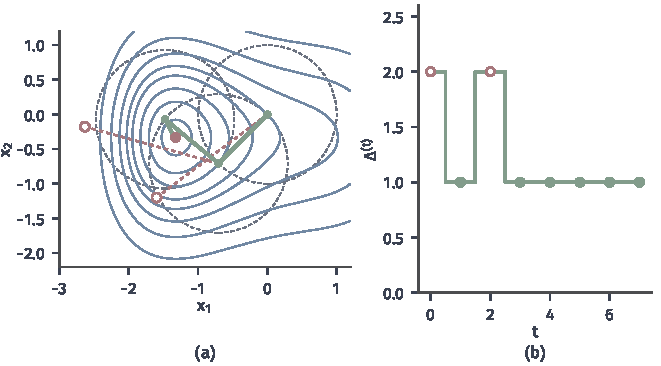
\includegraphics[width=112mm]{figures/05-optimization/02-smooth-optimization/matplotlib/tr-outer-path/figure.pdf}
 \caption{贯穿例子的完整运行。(a)~目标等高线（蓝）上的轨迹（绿），虚线圆是前几轮被接受时的信赖域，红色虚线和空心点是被拒绝的试探，红点是最小点。(b)~半径随轮数的变化，实心点表示接受，空心点表示拒绝。}
 \label{fig:tr-outer-path}
\end{BookInlineFigure}

这次运行显示了框架的分工：远离解时，半径起主导作用，负责把模型限制在可信的范围；靠近解时，半径不再起作用，方法退化成普通的Newton法。半径的调整不需要人工干预，由下降比自动完成。

\section{收敛与计算成本}
\label{sec:tr-convergence}

前几节的例子看起来都收敛了，在什么条件下这是必然的，极限点是什么样的点，每一轮又要花多少计算？

\paragraph{假设}
一阶结果需要下面三条假设。
\begin{enumerate}
 \item $f$连续可微，下有界，$f\geq f_{\mathrm{low}}$，梯度在$\mathbb{R}^n$上Lipschitz连续，常数为$L$。
 \item 模型矩阵一致有界：$\bm{B}^{(t)}$对称，$\lVert\bm{B}^{(t)}\rVert_2\leq M$，$M>0$。
 \item 候选步可行，$\lVert\bm{p}^{(t)}\rVert_2\leq\Delta^{(t)}$，并且对某个$c_1\in(0,1]$满足充分模型下降：
 \begin{equation}
  \operatorname{pred}(\bm{p}^{(t)})\geq c_1\lVert\bm{g}^{(t)}\rVert_2\min\Bigl\{\Delta^{(t)},\ \frac{\lVert\bm{g}^{(t)}\rVert_2}{M}\Bigr\}.
  \label{eq:tr-assumption-decrease}
 \end{equation}
\end{enumerate}

第三条由式~\eqref{eq:tr-sufficient-decrease}和$\lVert\bm{B}^{(t)}\rVert_2\leq M$推出，前面三种求解器都满足。第一条的全局Lipschitz条件可以放宽：目标~\eqref{eq:tr-example}的梯度不是全局Lipschitz的，但它的水平集有界，半径又有上限$\Delta_{\max}$，试探点都落在一个紧集内，$L$只需在这个紧集上成立。

条件里没有要求$\bm{B}^{(t)}$接近Hessian，也没有要求子问题解得精确。模型只要在一阶上与目标匹配，这正是拟牛顿模型能够进入这个框架的原因。

\paragraph{半径不会塌缩}
证明的核心是一个观察：半径足够小时，模型误差相对预测下降可以忽略，这一步一定被接受。模型误差是半径的二次量，预测下降却是半径的一次量，两者之比随半径趋于零。图~\ref{fig:tr-radius-rho}在点$\bm{a}$上验证了这一点：取精确Hessian时$\lvert1-\rho\rvert$随半径的斜率是$2$，取粗糙的$\bm{B}=\bm{I}$时斜率是$1$，后者正是定理使用的一般界。

\begin{BookInlineFigure}
 \centering
 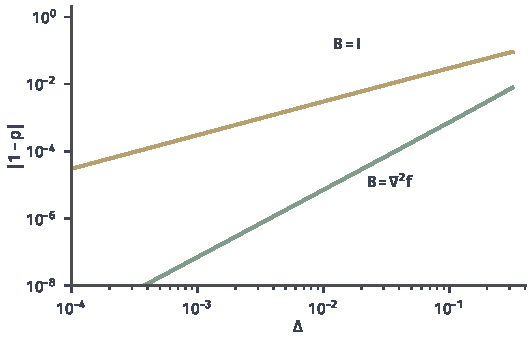
\includegraphics[width=90mm]{figures/05-optimization/02-smooth-optimization/matplotlib/tr-radius-rho/figure.pdf}
 \caption{在点$\bm{a}$沿负梯度方向取长度$\Delta$的步，$\lvert1-\rho\rvert$随$\Delta$的变化（对数坐标）。绿线的模型矩阵是Hessian，斜率约为$2$；黄线的模型矩阵是$\bm{I}$，斜率约为$1$。两条线都随$\Delta\to0$趋于零。}
 \label{fig:tr-radius-rho}
\end{BookInlineFigure}

\begin{theorem}[梯度的下极限为零]
 \label{thm:tr-first-order}
 在上述三条假设下，设外层迭代按式~\eqref{eq:tr-accept}和式~\eqref{eq:tr-radius}更新，其中$\eta_1>0$。此时
 \begin{equation}
  \liminf_{t\to\infty}\lVert\bm{g}^{(t)}\rVert_2=0.
  \label{eq:tr-liminf}
 \end{equation}
\end{theorem}

\begin{proof}
 反设存在$\varepsilon>0$和$T_0$，使得$t\geq T_0$时$\lVert\bm{g}^{(t)}\rVert_2\geq\varepsilon$。

 第一步估计模型误差。由梯度Lipschitz连续，对任意$\bm{p}$，
 \[
  \bigl\lvert f(\bm{x}+\bm{p})-f(\bm{x})-\langle\bm{g},\bm{p}\rangle\bigr\rvert
  =\Bigl\lvert\int_0^1\langle\nabla f(\bm{x}+s\bm{p})-\bm{g},\bm{p}\rangle\,\mathrm{d}s\Bigr\rvert
  \leq\frac{L}{2}\lVert\bm{p}\rVert_2^2.
 \]
 再计入模型的二次项，且$\lVert\bm{p}^{(t)}\rVert_2\leq\Delta^{(t)}$，得到
 \[
  \bigl\lvert f(\bm{x}^{(t)}+\bm{p}^{(t)})-m^{(t)}(\bm{p}^{(t)})\bigr\rvert\leq\frac{L+M}{2}(\Delta^{(t)})^2.
 \]

 第二步说明小半径时不会缩小。令
 \[
  K=\min\Bigl\{\frac1M,\ \frac{2c_1(1-\eta_2)}{L+M}\Bigr\}.
 \]
 设$t\geq T_0$且$\Delta^{(t)}\leq K\varepsilon$。此时$\Delta^{(t)}\leq\varepsilon/M$，不超过$\lVert\bm{g}^{(t)}\rVert_2/M$，所以式~\eqref{eq:tr-assumption-decrease}的最小值取在$\Delta^{(t)}$上：
 \[
  \operatorname{pred}(\bm{p}^{(t)})\geq c_1\varepsilon\Delta^{(t)}.
 \]
 又$m^{(t)}(\bm{0})=f(\bm{x}^{(t)})$，所以预测下降与实际下降之差就是模型误差，于是
 \[
  \lvert1-\rho^{(t)}\rvert\leq\frac{(L+M)(\Delta^{(t)})^2/2}{c_1\varepsilon\Delta^{(t)}}=\frac{(L+M)\Delta^{(t)}}{2c_1\varepsilon}\leq1-\eta_2.
 \]
 因此$\rho^{(t)}\geq\eta_2\geq\eta_1$，这一轮半径不缩小。

 第三步得到半径的下界。半径只在$\Delta^{(t)}>K\varepsilon$时才可能缩小，缩小后不低于$\theta K\varepsilon$，所以对$t\geq T_0$，
 \[
  \Delta^{(t)}\geq\Delta_{\min}:=\min\{\Delta^{(T_0)},\ \theta K\varepsilon\}>0.
 \]

 第四步导出矛盾。若被接受的轮只有有限多次，则此后点不动，半径每轮乘以$\theta$，趋于零，与下界矛盾。所以接受无穷多次，每次接受时$\rho^{(t)}\geq\eta_1$，并由式~\eqref{eq:tr-assumption-decrease}，
 \[
  f(\bm{x}^{(t)})-f(\bm{x}^{(t+1)})\geq\eta_1\operatorname{pred}(\bm{p}^{(t)})
  \geq\eta_1c_1\varepsilon\min\Bigl\{\Delta_{\min},\ \frac{\varepsilon}{M}\Bigr\}>0.
 \]
 目标值单调不增，却无穷多次下降一个固定的量，这与$f\geq f_{\mathrm{low}}$矛盾。
\end{proof}

下极限只说明有一个子列的梯度趋于零。$\eta_1>0$时可以加强：整个序列的梯度都趋于零。

\begin{theorem}[梯度趋于零]
 \label{thm:tr-limit}
 在定理~\ref{thm:tr-first-order}的条件下，
 \begin{equation}
  \lim_{t\to\infty}\lVert\bm{g}^{(t)}\rVert_2=0.
  \label{eq:tr-limit}
 \end{equation}
\end{theorem}

\begin{proof}
 反设存在$\varepsilon>0$和无穷多个下标$t$满足$\lVert\bm{g}^{(t)}\rVert_2\geq2\varepsilon$。对每个这样的$t$，由定理~\ref{thm:tr-first-order}，存在最小的$l(t)>t$使$\lVert\bm{g}^{(l(t))}\rVert_2<\varepsilon$。在$t\leq k<l(t)$的轮中$\lVert\bm{g}^{(k)}\rVert_2\geq\varepsilon$。记其中被接受的轮的集合为$\mathcal{K}$。

 由Lipschitz条件和$\lVert\bm{p}^{(k)}\rVert_2\leq\Delta^{(k)}$，这段路程的总长度不能太短：
 \[
  \varepsilon\leq\lVert\bm{g}^{(t)}\rVert_2-\lVert\bm{g}^{(l(t))}\rVert_2\leq L\sum_{k\in\mathcal{K}}\lVert\bm{p}^{(k)}\rVert_2\leq L\sum_{k\in\mathcal{K}}\Delta^{(k)}.
 \]

 这段路程上目标的下降量由接受规则和式~\eqref{eq:tr-assumption-decrease}控制：
 \[
  f(\bm{x}^{(t)})-f(\bm{x}^{(l(t))})\geq\eta_1c_1\varepsilon\sum_{k\in\mathcal{K}}\min\Bigl\{\Delta^{(k)},\ \frac{\varepsilon}{M}\Bigr\}.
 \]

 若$\mathcal{K}$中某一项有$\Delta^{(k)}>\varepsilon/M$，右端至少是$\eta_1c_1\varepsilon^2/M$。否则右端等于$\eta_1c_1\varepsilon\sum\Delta^{(k)}$，至少是$\eta_1c_1\varepsilon^2/L$。两种情形下降量都有一个不依赖$t$的正下界。但$f(\bm{x}^{(t)})$单调且有下界，$t\to\infty$时$f(\bm{x}^{(t)})-f(\bm{x}^{(l(t))})\to0$，矛盾。
\end{proof}

条件的作用可以逐条核对。去掉下有界，目标可以一直下降，例如$f(x)=-x$，梯度恒为$-1$。去掉$\eta_1>0$的接受门槛，只要求$\rho^{(t)}>0$，下降量可以任意小，一般只能得到下极限的结论。去掉充分模型下降，候选步可以小到没有进展，比值$\rho^{(t)}$即使接近$1$也无济于事。

\paragraph{二阶保证}
定理~\ref{thm:tr-limit}只说明极限点是驻点，鞍点也是驻点。要排除负曲率，候选步必须真正使用负曲率。设$\bm{B}^{(t)}=\bm{H}^{(t)}$，用下面的量衡量负曲率的大小：
\[
 \lambda^{(t)}_-=\max\{0,\ -\lambda_{\min}(\bm{H}^{(t)})\}.
\]
要求存在常数$c_2>0$，使得
\begin{equation}
 \operatorname{pred}(\bm{p}^{(t)})\geq c_2\lambda^{(t)}_-(\Delta^{(t)})^2.
 \label{eq:tr-eigen-decrease}
\end{equation}

子问题的全局解满足这一条，$c_2=1/2$。取$\bm{u}$是$\lambda_{\min}$的单位特征向量，选符号使$\langle\bm{g},\bm{u}\rangle\leq0$，点$\Delta\bm{u}$可行，由它的模型值得
\[
 m(\bm{0})-m(\Delta\bm{u})=-\Delta\langle\bm{g},\bm{u}\rangle-\frac12\lambda_{\min}\Delta^2\geq\frac12\lambda_-\Delta^2,
\]
全局解的预测下降不低于这个量。

Cauchy步和截断共轭梯度不满足式~\eqref{eq:tr-eigen-decrease}。第~\ref{sec:tr-model}节困难情形的数据$\bm{g}=(0,1)^\top$，$\bm{B}=\operatorname{diag}(-1,3)$，$\Delta=1$就是反例。截断共轭梯度第一步$\bm{d}^{(0)}=(0,-1)^\top$，曲率为正，一步到$(0,-1/3)^\top$，残差为零而停止，预测下降只有$1/6$。全局解的预测下降是$5/8$，并且沿$\bm{e}_1$方向使用了负曲率。迭代只在Krylov子空间中进行，而这个子空间恰好与$\bm{e}_1$正交，图~\ref{fig:tr-second-order}(a)画出了这一点。若$\bm{g}=\bm{0}$，迭代第一步就停在$\bm{p}=\bm{0}$，负曲率完全看不到。

\begin{theorem}[二阶下极限]
 \label{thm:tr-second-order}
 在定理~\ref{thm:tr-first-order}的条件之外，设$\bm{B}^{(t)}=\bm{H}^{(t)}$，Hessian是$L_H$-Lipschitz的，且候选步满足式~\eqref{eq:tr-eigen-decrease}。则
 \begin{equation}
  \liminf_{t\to\infty}\max\bigl\{\lVert\bm{g}^{(t)}\rVert_2,\ \lambda^{(t)}_-\bigr\}=0.
  \label{eq:tr-second-order}
 \end{equation}
\end{theorem}

\begin{proof}
 反设存在$\varepsilon>0$和$T_0$，使得$t\geq T_0$时
 \[
  \max\{\lVert\bm{g}^{(t)}\rVert_2,\ \lambda^{(t)}_-\}\geq\varepsilon.
 \]
 若$\lVert\bm{g}^{(t)}\rVert_2\geq\varepsilon$，定理~\ref{thm:tr-first-order}证明的第二步依然适用。若$\lambda^{(t)}_-\geq\varepsilon$，由Hessian的Lipschitz条件，模型误差不超过$L_H\lVert\bm{p}\rVert_2^3/6$，再用式~\eqref{eq:tr-eigen-decrease}，
 \[
  \lvert1-\rho^{(t)}\rvert\leq\frac{L_H(\Delta^{(t)})^3/6}{c_2\varepsilon(\Delta^{(t)})^2}=\frac{L_H\Delta^{(t)}}{6c_2\varepsilon}.
 \]
 所以取$K_2=\min\{K,\ 6c_2(1-\eta_2)/L_H\}$，$\Delta^{(t)}\leq K_2\varepsilon$时半径不缩小，同样得到半径的正下界$\Delta_{\min}$。每次接受至少下降
 \[
  \eta_1\min\Bigl\{c_1\varepsilon\min\bigl\{\Delta_{\min},\ \varepsilon/M\bigr\},\ c_2\varepsilon\Delta_{\min}^2\Bigr\}>0,
 \]
 与定理~\ref{thm:tr-first-order}证明的第四步一样导出矛盾。
\end{proof}

这个定理给出的是一个子列上的结论：若该子列有极限点$\bar{\bm{x}}$，则$\nabla f(\bar{\bm{x}})=\bm{0}$且$\nabla^2f(\bar{\bm{x}})\succeq\bm{0}$。这只是二阶必要条件，并不说明$\bar{\bm{x}}$是局部极小点。图~\ref{fig:tr-second-order}(b)的$f(x)=x^3$在$x=0$处梯度和Hessian都为零，从这一点出发，任何候选步都不能使模型下降，算法立即停止，而这个点不是局部极小点。

$x^3$没有下界，这里只用它展示驻点附近的形状；把函数在远处改成有下界、导数Lipschitz的光滑函数，$x=0$附近的情形不变。

所以不能仅凭采用信赖域就声称找到了局部极小点，更谈不上全局最优。一阶保证只需要充分模型下降，二阶保证要求候选步真正利用负曲率，两者对子问题的精度要求不同。这种差别在第~\ref{chap:saddle-points}章有进一步的讨论。

\begin{BookInlineFigure}
 \centering
 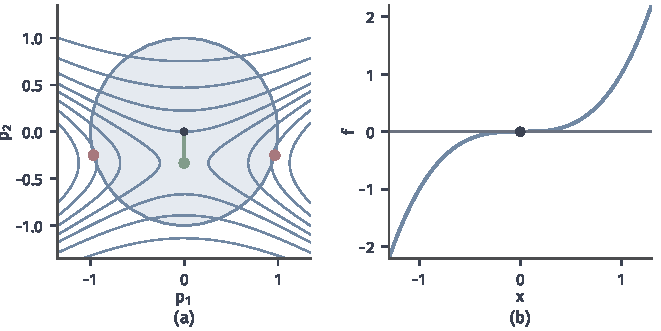
\includegraphics[width=112mm]{figures/05-optimization/02-smooth-optimization/matplotlib/tr-second-order/figure.pdf}
 \caption{二阶保证的两个边界。(a)~模型$\bm{g}=(0,1)^\top$，$\bm{B}=\operatorname{diag}(-1,3)$，$\Delta=1$：截断共轭梯度只沿$p_2$轴走到绿点，两个红点是全局解。(b)~$f(x)=x^3$，黑点处梯度和Hessian都为零，满足二阶必要条件，却不是局部极小点。}
 \label{fig:tr-second-order}
\end{BookInlineFigure}

\paragraph{迭代次数}
定理~\ref{thm:tr-first-order}的证明本身给出了复杂度。设前$T$轮都有$\lVert\bm{g}^{(t)}\rVert_2\geq\varepsilon$，半径有下界$\Delta_{\min}$，$\varepsilon$小时$\Delta_{\min}$与$\varepsilon$同阶。把第四步中每次接受的下降量代入总下降量$f(\bm{x}^{(0)})-f_{\mathrm{low}}$，可知接受的轮数$A$满足
\begin{equation}
 A\leq\frac{f(\bm{x}^{(0)})-f_{\mathrm{low}}}{\eta_1c_1\varepsilon\min\{\Delta_{\min},\ \varepsilon/M\}}=O(\varepsilon^{-2}).
 \label{eq:tr-accepted-count}
\end{equation}

拒绝的轮数$R$也受控制。半径每次接受至多乘以$2$，每次拒绝乘以$\theta$，且始终不低于$\Delta_{\min}$，所以$\Delta^{(0)}2^A\theta^R\geq\Delta_{\min}$，由此得到
\begin{equation}
 R\leq\frac{A\ln2+\ln(\Delta^{(0)}/\Delta_{\min})}{\ln(1/\theta)}.
 \label{eq:tr-rejected-count}
\end{equation}

因此外层总轮数是$O(\varepsilon^{-2})$，只比接受轮数多一个常数倍和一个对数项。这个阶与梯度下降相同，并且对信赖域Newton法也是紧的，构造最坏的目标需要专门设计的例子，篇幅较长，读者可查阅专门的优化复杂度文献。这也提醒我们，信赖域Newton法在实践中的优势来自局部收敛和对曲率的利用，不来自这个最坏情形的上界。

\paragraph{局部收敛}
设$\bm{x}^{(t)}\to\bm{x}^\star$，$\nabla^2f(\bm{x}^\star)\succ\bm{0}$，Hessian在$\bm{x}^\star$附近Lipschitz，并取$\bm{B}^{(t)}=\bm{H}^{(t)}$。靠近解时Newton步趋于零，比值$\rho^{(t)}$趋于$1$，半径不再缩小，Newton步终将落在球内。狗腿法、精确解都直接取Newton步，于是回到第~\ref{chap:second-order-methods}章的局部二次收敛。截断共轭梯度由残差停止，$\eta\to0$的快慢决定超线性或二次收敛，取$\eta=\min\{0.1,\sqrt{\lVert\bm{g}\rVert_2}\}$时是超线性的。表~\ref{tab:tr-history}中第$4$到第$7$轮就是这一阶段。这里只说明了机制，严格的证明还需要验证$\rho^{(t)}\to1$的速度，读者可查阅\scite{math-nocedal2006numerical}。

\paragraph{计算成本}
评价信赖域的成本要把外层和内层分开算，表~\ref{tab:tr-cost}按一次子问题列出。

\begin{BookInlineTable}
 \centering
 \begin{tabular}{lll}
  \toprule
  子问题解法 & 对$\bm{B}$的要求 & 一次求解的代价\\
  \midrule
  Cauchy步 & 对称 & $1$次矩阵向量乘积\\
  狗腿法 & 正定 & $1$次分解，约$n^3/3$\\
  截断共轭梯度 & 对称 & $j$次矩阵向量乘积，$j\leq n$\\
  精确解 & 对称 & 数次分解，约$n^3/3$每次\\
  \bottomrule
 \end{tabular}
 \caption{一次子问题的代价，稠密矩阵，只计主要运算。}
 \label{tab:tr-cost}
\end{BookInlineTable}

外层每一轮需要一次函数值$f(\bm{x}^{(t)}+\bm{p}^{(t)})$；只有被接受的轮才需要新的梯度和$\bm{B}$，拒绝的轮只多一次子问题和一次函数值。Hessian向量乘积不必形成整个矩阵，用梯度差近似时，一次乘积大约是一次梯度的代价：
\begin{equation}
 \bm{H}^{(t)}\bm{v}\approx\frac{\nabla f(\bm{x}^{(t)}+h\bm{v})-\nabla f(\bm{x}^{(t)})}{h}.
 \label{eq:tr-hessian-vector}
\end{equation}
所以比较方法时不能只看外层轮数，要把内层的乘积次数也算进去。拒绝也不是免费的：当函数值很贵时，半径初值和更新因子要避免频繁试探。

图~\ref{fig:tr-methods-compare}是一个$n=20$的实验，目标是
\[
 f(\bm{x})=\sum_{i=1}^{19}\bigl[10(x_{i+1}-x_i^2)^2+(1-x_i)^2\bigr].
\]
三种方法的外层框架相同，参数同前。精确Hessian配截断共轭梯度用$26$个外层轮次、$157$次Hessian向量乘积把梯度降到$10^{-7}$以下。SR1模型从$20\bm{I}$出发，用$90$轮，每轮要多算一次梯度，但完全不用Hessian。只用Cauchy步时，$1200$轮后梯度仍有$1.8\times10^{-4}$。三者都满足第~\ref{sec:tr-convergence}节开头的假设，收敛定理对它们一视同仁，实际差距来自模型和子问题利用了多少曲率。

\begin{BookInlineFigure}
 \centering
 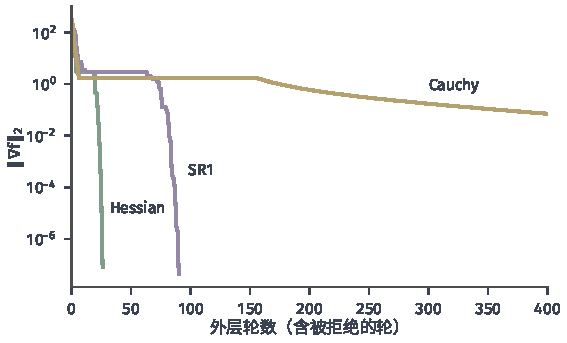
\includegraphics[width=96mm]{figures/05-optimization/02-smooth-optimization/matplotlib/tr-methods-compare/figure.pdf}
 \caption{同一信赖域框架下三种选择的梯度范数（到当前轮为止的最小值，对数坐标）。绿线是Hessian配截断共轭梯度，紫线是SR1模型配截断共轭梯度，黄线是Hessian配Cauchy步。横轴的轮数包含被拒绝的轮。目标是正文中的$20$维函数，每个奇数位分量初值为$-1.2$，其余为$1$。}
 \label{fig:tr-methods-compare}
\end{BookInlineFigure}

\section{本章小结}
\label{sec:tr-summary}

本章开头的问题是：局部模型只在附近可靠，怎样同时决定往哪里走、走多远。信赖域的回答是把两件事合并成一个带半径约束的子问题，半径表示当前愿意相信模型的范围。这样即使曲率矩阵不定，子问题也有解，负曲率不必被修正掉，反而可以把步推向边界。

子问题的全局解由一个平移过的线性方程刻画，但外层迭代并不需要它。Cauchy步给出充分模型下降的下限，狗腿法在$\bm{B}$正定时用两段折线逼近解的轨迹，截断共轭梯度只用矩阵向量乘积，并用边界和曲率两条规则处理信赖域带来的新情况。

下降比$\rho^{(t)}$把模型的预测和目标的实际下降作比较，决定接受这一步以及下一轮的半径。拒绝时点不动，模型沿用，只在更小的范围内重解。

收敛分析的条件和结论要分开记。目标下有界、梯度Lipschitz、模型有界、充分模型下降，这四条保证梯度趋于零，外层轮数是$O(\varepsilon^{-2})$，并不要求精确的Hessian。取精确Hessian并要求候选步利用负曲率，才有二阶必要条件的保证，而这仍不等于找到局部极小点，更不等于全局最优。

表~\ref{tab:tr-summary}把三种子问题解法放在一起。

\begin{BookInlineTable}
 \centering
 \begin{tabular}{llll}
  \toprule
  解法 & $\bm{B}$的要求 & 主要代价 & 负曲率\\
  \midrule
  Cauchy步 & 对称 & 一次乘积 & 只看负梯度方向\\
  狗腿法 & 正定 & 一次分解 & 不能处理\\
  截断共轭梯度 & 对称 & 若干次乘积 & 遇到时走到边界\\
  全局解 & 对称 & 数次分解 & 完整利用\\
  \bottomrule
 \end{tabular}
 \caption{子问题几种解法的对照。}
 \label{tab:tr-summary}
\end{BookInlineTable}

最后一列是第~\ref{chap:saddle-points}章的入口。模型处理负曲率的能力只是工具，梯度很小时所得驻点属于哪一种，怎样可靠地离开鞍点，要在那里进一步明确。


\chapter{鞍点的处理}
\label{chap:saddle-points}

一个算法运行结束，报告梯度范数只有$0.06$。这句话能说明什么？地面在这里几乎是平的，可是平的地方不止谷底，山顶和山口也是平的。下降算法走到山口附近，脚下坡度变得很小，步子随之变小，看起来像是快要到达终点，其实旁边还有一条向下的路。

非凸目标里，这种情形不是例外。第~\ref{chap:first-order-methods}章到第~\ref{chap:trust-region}章的保证，多数只说梯度趋于零。本章追问这以后的事：梯度已经很小时，怎样知道目标还能不能继续下降，怎样真正下降，最后又能声称得到了什么样的点。

全章用同一个二维目标把这些问题算到底。先把梯度为零的点分类，看清二阶信息能排除什么、还留下什么。然后讨论怎样只靠Hessian向量积找到向下弯曲的方向，并分清“找到”和“没有找到”分别能得出什么结论。

接着比较三种离开的办法：已知向下弯曲的方向时沿它走一步；只有梯度时给迭代点一点随机扰动；手里有二次模型时保留它的不定性。最后把停止条件和计算成本放在一起，说明一次运行究竟可以报告什么样的保证。

\section{驻点的类型}
\label{sec:saddle-types}

梯度为零的点有哪几类，二阶信息能把它们分开到什么程度？先用一个具体的目标看清这些点的样子，再给定义，然后专门讨论二阶信息判断不了的情形。

\paragraph{贯穿全章的例子}
我们用下面这个目标，它在$x_1$方向是一口双井，在$x_2$方向是一只碗：
\begin{equation}
 f(\bm{x})=\frac14\bigl(x_1^2-1\bigr)^2+\frac12x_2^2.
 \label{eq:saddle-example}
\end{equation}
它的梯度和Hessian可以直接写出：
\begin{equation}
 \nabla f(\bm{x})=\begin{bmatrix}x_1^3-x_1\\x_2\end{bmatrix},\qquad
 \nabla^2 f(\bm{x})=\begin{bmatrix}3x_1^2-1&0\\0&1\end{bmatrix}.
 \label{eq:saddle-example-derivatives}
\end{equation}

令梯度为零，第二个分量给出$x_2=0$，第一个分量给出$x_1(x_1^2-1)=0$。于是有三个驻点，它们的目标值和Hessian是
\[
 \begin{aligned}
 (\pm1,0):&\quad f=0,\quad \nabla^2f=\operatorname{diag}(2,1),\\
 (0,0):&\quad f=\tfrac14,\quad \nabla^2f=\operatorname{diag}(-1,1).
 \end{aligned}
\]

$f\geq0$处处成立，所以$(\pm1,0)$是全局最优解。原点沿$x_2$方向是最低点，沿$x_1$方向是最高点，这正是一个山口。图~\ref{fig:saddle-running-landscape}画出了等高线和$x_2=0$上的截面。

\begin{BookInlineFigure}
  \centering
  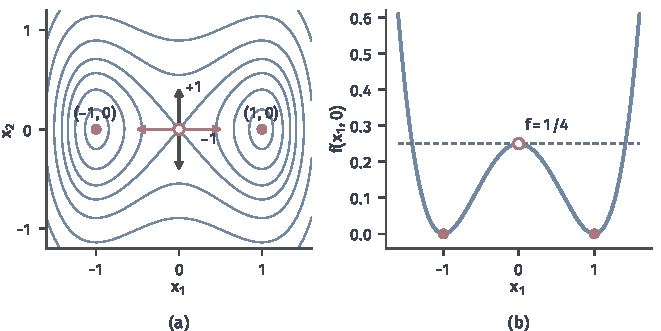
\includegraphics[width=112mm]{figures/05-optimization/02-smooth-optimization/matplotlib/saddle-running-landscape/figure.pdf}
  \caption{目标~\eqref{eq:saddle-example}。(a)蓝线是等高线，红点是两个全局最优解，空心点是原点处的鞍点，红色箭头是曲率为$-1$的方向，灰色箭头是曲率为$+1$的方向。(b)$x_2=0$上的截面，鞍点位于两口井之间的高处，函数值为$1/4$。}
  \label{fig:saddle-running-landscape}
\end{BookInlineFigure}

后面的分析要用到两个常数。Hessian~\eqref{eq:saddle-example-derivatives}的元素随$x_1$增长，全局的常数不存在，所以我们只在带形区域上讨论：
\[
 \bm{U}=\bigl\{\bm{x}\in\mathbb{R}^2:\ \lvert x_1\rvert\leq1\bigr\}.
\]

在$\bm{U}$上，$3x_1^2-1$介于$-1$与$2$之间，因此谱范数$\lVert\nabla^2f\rVert_2\leq2$，光滑常数取$L=2$。Hessian本身的变化由差值控制：
\[
 \bigl\lvert(3x_1^2-1)-(3y_1^2-1)\bigr\rvert
 =3\lvert x_1+y_1\rvert\,\lvert x_1-y_1\rvert
 \leq6\lvert x_1-y_1\rvert.
\]
所以在$\bm{U}$上，Hessian满足下面的Lipschitz条件，常数$M=6$：
\[
 \bigl\lVert\nabla^2f(\bm{x})-\nabla^2f(\bm{y})\bigr\rVert_2\leq M\lVert\bm{x}-\bm{y}\rVert_2.
\]
全章固定步长取$\alpha=1/L=1/2$。

\paragraph{三类驻点}
站在驻点上，一阶变化消失了，目标的走势由Hessian决定。由Taylor公式，对小的$\bm{h}$，
\[
 f(\bm{x}+\bm{h})-f(\bm{x})=\frac12\bm{h}^\top\nabla^2f(\bm{x})\bm{h}+o\bigl(\lVert\bm{h}\rVert_2^2\bigr).
\]
量$\bm{h}^\top\nabla^2f(\bm{x})\bm{h}$的符号回答了“沿这个方向向上弯还是向下弯”。按照能否找到向下弯的方向，驻点分成下面几类。

\begin{definition}[驻点的类型]
 \label{def:saddle-stationary}
 设$f$二阶连续可微。若点$\bm{x}$满足
 \begin{equation}
  \nabla f(\bm{x})=\bm{0},
  \label{eq:saddle-first-order}
 \end{equation}
 就称它为\term{一阶驻点}（first-order stationary point）。若还满足
 \begin{equation}
  \nabla^2f(\bm{x})\succeq\bm{0},
  \label{eq:saddle-second-order}
 \end{equation}
 就称它为\term{二阶驻点}（second-order stationary point）。若一阶驻点满足
 \begin{equation}
  \lambda_{\min}\bigl(\nabla^2f(\bm{x})\bigr)<0,
  \label{eq:saddle-strict}
 \end{equation}
 就称它为\term{严格鞍点}（strict saddle point）。
\end{definition}

一阶驻点要么是二阶驻点，要么是严格鞍点，两者互斥。名称上有一点需要留意：局部极大点也满足式~\eqref{eq:saddle-strict}，在这个约定下同样算作严格鞍点。原因是算法只关心有没有向下弯的方向，而局部极大点和山口在这一点上没有区别。

二阶条件告诉我们这些类别和局部极小点的关系。第~\ref{chap:optimization}章证明过：局部极小点必须是二阶驻点；Hessian正定的一阶驻点一定是严格局部极小点。因此严格鞍点一定不是局部极小点，而二阶驻点之中，Hessian正定的部分一定是局部极小点。

表~\ref{tab:saddle-origin-types}列出几个函数在原点的情形，它们的梯度在原点都为零。前两行是这两条结论直接判定的情形，后三行的Hessian半正定且奇异，正是二阶条件留下的缺口。

\begin{BookInlineTable}
  \centering
  \begin{tabular}{@{}lll@{}}
    \toprule
    函数 & 原点的Hessian & 原点的类型\\
    \midrule
    $x_1^2+x_2^2$ & $\operatorname{diag}(2,2)$ & 严格局部极小点\\
    $x_1^2-x_2^2$ & $\operatorname{diag}(2,-2)$ & 严格鞍点\\
    $x_1^2+x_2^4$ & $\operatorname{diag}(2,0)$ & 二阶驻点，局部极小点\\
    $x_1^2-x_2^4$ & $\operatorname{diag}(2,0)$ & 二阶驻点，不是局部极小点\\
    $x_1^4-x_2^4$ & $\bm{0}$ & 二阶驻点，不是局部极小点\\
    \bottomrule
  \end{tabular}
  \caption{原点处的几种情形。第三行与第四行的梯度和Hessian完全相同，类型却不同。}
  \label{tab:saddle-origin-types}
\end{BookInlineTable}

\paragraph{退化情形}
Hessian半正定仍不足以说明是局部极小点。比较$x_1^2+x_2^4$和$x_1^2-x_2^4$：它们在原点的函数值、梯度和Hessian完全一样，差别只在四阶项。沿$x_2$轴看，
\[
 x_1^2+x_2^4\big|_{x_1=0}=t^4,\qquad
 x_1^2-x_2^4\big|_{x_1=0}=-t^4.
\]

前者把原点托在最低处，后者从原点沿$x_2$轴一直下降。只看到二阶为止的信息，这两个函数无法分开。图~\ref{fig:saddle-stationary-zoo}用浅红色标出比原点函数值更低的区域，只要原点的任意小邻域内有浅红色，原点就不是局部极小点。

\begin{BookInlineFigure}
  \centering
  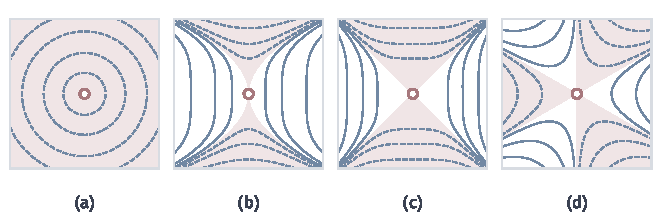
\includegraphics[width=112mm]{figures/05-optimization/02-smooth-optimization/matplotlib/saddle-stationary-zoo/figure.pdf}
  \caption{原点处四种不是局部极小点的驻点，蓝线是等高线，虚线为负值，浅红区域是函数值低于$f(\bm{0})=0$的点。(a)$-x_1^2-x_2^2$，局部极大点。(b)$x_1^2-x_2^4$，Hessian为$\operatorname{diag}(2,0)$。(c)$x_1^4-x_2^4$，Hessian为零。(d)$x_1^3-3x_1x_2^2$，Hessian为零。后三个都没有负曲率，算法靠Hessian察觉不到下降方向。}
  \label{fig:saddle-stationary-zoo}
\end{BookInlineFigure}

图中(a)的负曲率是显式的，(b)、(c)、(d)的下降则藏在更高阶的项里。(d)沿$x_1$轴的函数值是$t^3$，经过原点时由正变负，下降的一侧和上升的一侧挨在一起。

\paragraph{每条直线上都最低，仍然不是局部极小}
有人会想：既然二阶信息只看直线方向，那么补上高阶项，逐条直线检查目标是否在原点取到局部最低，总该够了吧？下面的例子说明还是不够：
\begin{equation}
 f(\bm{x})=\bigl(x_2-x_1^2\bigr)\bigl(x_2-2x_1^2\bigr).
 \label{eq:saddle-peano}
\end{equation}

展开得到$x_2^2-3x_1^2x_2+2x_1^4$，所以原点是驻点，Hessian是$\operatorname{diag}(0,2)$。先看经过原点的每条直线。沿$x_2=mx_1$，目标是
\[
 f(t,mt)=m^2t^2-3mt^3+2t^4.
\]

$m\neq0$时二次项为正，$t$足够小时函数值为正。$m=0$时是$2t^4$，沿$x_2$轴是$x_2^2$，也都大于零。所以原点在每条直线上都是严格局部最低点。

可是沿抛物线$x_2=\tfrac32x_1^2$走，两个因子一正一负：
\[
 f\bigl(t,\tfrac32t^2\bigr)=\Bigl(\tfrac12t^2\Bigr)\Bigl(-\tfrac12t^2\Bigr)=-\frac14t^4<0.
\]

原点的任意小邻域内都有比它更低的点，所以它不是局部极小点。图~\ref{fig:saddle-peano}(a)给出了几何解释：函数值为负的区域夹在两条抛物线之间，而任何一条直线在原点附近都会离开这个弯曲的窄缝。沿直线下降的想法，在这里看不到弯曲的下降路径。

\begin{BookInlineFigure}
  \centering
  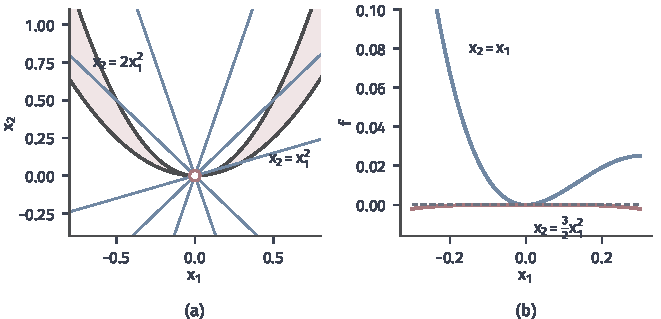
\includegraphics[width=112mm]{figures/05-optimization/02-smooth-optimization/matplotlib/saddle-peano/figure.pdf}
  \caption{目标~\eqref{eq:saddle-peano}。(a)浅红色是$f<0$的区域，夹在抛物线$x_2=x_1^2$和$x_2=2x_1^2$之间；蓝色直线在原点附近都位于这个区域之外。(b)沿直线$x_2=x_1$的函数值（蓝）在原点取最低，沿抛物线$x_2=\tfrac32x_1^2$的函数值（红）为负。}
  \label{fig:saddle-peano}
\end{BookInlineFigure}

\paragraph{二阶条件能排除什么}
把这些类别按包含关系排列，得到图~\ref{fig:saddle-class-nesting}。每往里一层，条件就强一些。

\begin{BookInlineFigure}
  \centering
  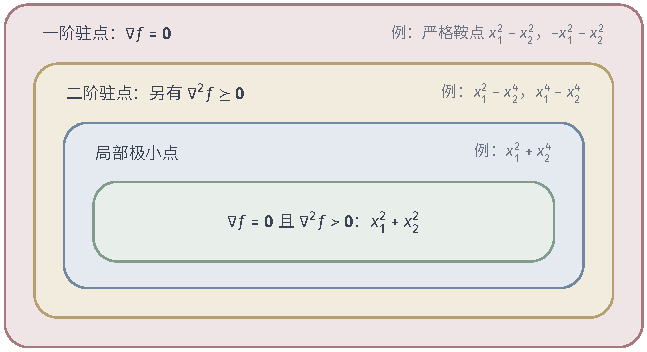
\includegraphics[width=109.6mm]{figures/05-optimization/02-smooth-optimization/tikz/saddle-class-nesting/figure.pdf}
  \caption{驻点类别的包含关系，每层右上角的函数在原点属于该层而不属于更内一层。最外层与第二层之间的差就是严格鞍点。第二层与第三层之间是退化的二阶驻点，二阶信息无法把它们和局部极小点分开。}
  \label{fig:saddle-class-nesting}
\end{BookInlineFigure}

由此可以说清楚二阶信息的能力。负特征值是确凿的证据：只要算出一个负的曲率，就能断定这里不是局部极小点。Hessian正定也是确凿的证据：这里一定是严格局部极小点。两者之间的情形，二阶信息保持沉默，并不是“大概是极小点”的意思。

所以算法的目标要说得克制。排除严格鞍点是可以做到的事，这是后面几节的内容。判定一个退化的二阶驻点是否为局部极小点，一般需要更高阶的信息，本章的方法不处理。

\paragraph{局部条件不说明全局}
上面的讨论还停留在局部。即使某点确实是局部极小点，也不说明它是全局最优解。看下面这个倾斜的双井：
\[
 \psi(x)=\frac14x^4+\frac13x^3-x^2,\qquad
 \psi'(x)=x(x-1)(x+2).
\]

三个驻点的二阶导数由$\psi''(x)=3x^2+2x-2$算出：
\[
 \psi''(0)=-2,\qquad\psi''(1)=3,\qquad\psi''(-2)=6.
\]

$x=1$是严格局部极小点，满足所有局部条件，函数值却是$-5/12$，而全局最优解$x=-2$的函数值是$-8/3$。图~\ref{fig:saddle-tilted-well}中，从$x=1$到更低的井要先翻过$x=0$处的高坡。站在黄点上，任何只依赖当地导数的判据都看不到另一口井。

\begin{BookInlineFigure}
  \centering
  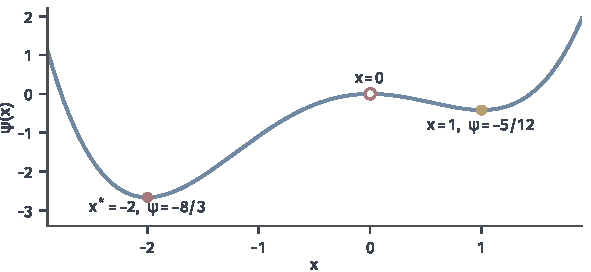
\includegraphics[width=100mm]{figures/05-optimization/02-smooth-optimization/matplotlib/saddle-tilted-well/figure.pdf}
  \caption{倾斜双井$\psi(x)=x^4/4+x^3/3-x^2$。黄点$x=1$是严格局部极小点，红点$x=-2$是全局最优解，空心点$x=0$是局部极大点。局部条件在黄点全部满足。}
  \label{fig:saddle-tilted-well}
\end{BookInlineFigure}

所以本章的“离开鞍点”只是把严格鞍点从可能的终点中排除。它既不判定退化的二阶驻点，也不保证到达全局最优解。


\section{负曲率的检测}
\label{sec:saddle-detection}

梯度已经很小时，怎样判断Hessian还有没有足够负的方向？变量很多时存不下Hessian，所以我们特别关心只用Hessian向量积能走多远，以及找到方向和没找到方向分别说明了什么。

\paragraph{要找的是什么}
对单位向量$\bm{v}$，Rayleigh商$R(\bm{v})=\bm{v}^\top\bm{H}\bm{v}$就是目标沿$\bm{v}$的曲率。谱分解$\bm{H}=\sum_i\lambda_i\bm{q}_i\bm{q}_i^\top$（特征值$\lambda_1\leq\cdots\leq\lambda_n$）给出
\begin{equation}
 \min_{\lVert\bm{v}\rVert_2=1}R(\bm{v})=\lambda_1=\lambda_{\min}(\bm{H}),
 \label{eq:saddle-rayleigh}
\end{equation}
最小值在$\bm{q}_1$处取到。

我们并不需要真的求出$\bm{q}_1$。只要有一个单位向量使$R(\bm{v})\leq-\gamma$，其中$\gamma>0$，它就是负曲率方向，后面的下降分析用到的只是这个不等式。本章的$\gamma$始终表示负曲率的大小。

在原点，$\bm{H}=\operatorname{diag}(-1,1)$，取$\bm{v}=(\cos\theta,\sin\theta)$，Rayleigh商是
\[
 R(\bm{v})=-\cos^2\theta+\sin^2\theta=-\cos2\theta.
\]
夹角在$45^\circ$以内的方向全都是负曲率方向，夹角在$30^\circ$以内的方向满足$R\leq-1/2$。图~\ref{fig:saddle-curvature-cone}显示负曲率方向占据一整个锥，这是检测能够用粗糙办法完成的原因。

\begin{BookInlineFigure}
  \centering
  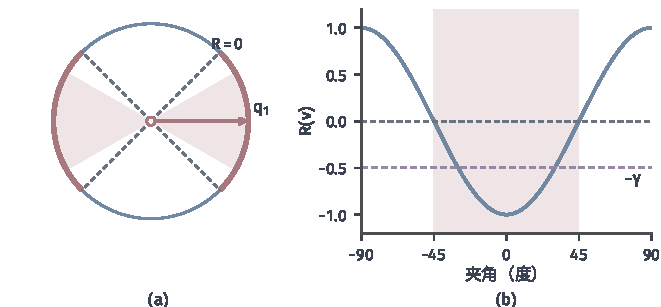
\includegraphics[width=112mm]{figures/05-optimization/02-smooth-optimization/matplotlib/saddle-curvature-cone/figure.pdf}
  \caption{$\bm{H}=\operatorname{diag}(-1,1)$的曲率随方向的变化。(a)单位圆上的红色弧是$R<0$的方向，浅红扇形是$R\leq-1/2$的方向，$\bm{q}_1$是最小特征向量。(b)$R$随方向与$\bm{q}_1$夹角的变化，浅红带是负曲率的范围，紫色虚线是阈值$-\gamma=-1/2$。}
  \label{fig:saddle-curvature-cone}
\end{BookInlineFigure}

\paragraph{矩阵存得下时}
$n$不大时，可以直接计算$\bm{H}$的特征分解，得到$\lambda_{\min}$和$\bm{q}_1$，运算量是$O(n^3)$。如果只需要回答“$\lambda_{\min}$是否大于$-\gamma$”，对$\bm{H}+\gamma\bm{I}$作Cholesky分解更省：分解成功当且仅当$\bm{H}+\gamma\bm{I}$正定，也就是$\lambda_{\min}>-\gamma$。

例中在原点取$\gamma=\tfrac12$，要分解的矩阵是
\[
 \bm{H}+\gamma\bm{I}=\operatorname{diag}\bigl(-\tfrac12,\tfrac32\bigr).
\]
第一个主元就是负的，分解失败，所以$\lambda_{\min}\leq-\tfrac12$。这种方法没有舍入以外的误差，结论是确定的，代价是要存下并分解整个矩阵。

\paragraph{矩阵存不下时}
第~\ref{chap:second-order-methods}章介绍过Hessian向量积，一次乘积的成本与一次梯度同量级。用自动微分可以精确得到它，用差分则只需要两次梯度：
\begin{equation}
 \hat{\bm{u}}=\frac{\nabla f(\bm{x}+h\bm{v})-\nabla f(\bm{x})}{h}.
 \label{eq:saddle-hvp-difference}
\end{equation}

差分带来的误差要记入账。设$\bm{v}$是单位向量，线段$[\bm{x},\bm{x}+h\bm{v}]$落在Hessian为$M$-Lipschitz的区域内。由微积分基本定理，
\[
 \nabla f(\bm{x}+h\bm{v})-\nabla f(\bm{x})-h\bm{H}\bm{v}
 =\int_0^h\bigl(\nabla^2f(\bm{x}+s\bm{v})-\nabla^2f(\bm{x})\bigr)\bm{v}\,\mathrm{d}s.
\]

被积函数的范数不超过$Ms$，积分得$Mh^2/2$。除以$h$，得到
\begin{equation}
 \lVert\hat{\bm{u}}-\bm{H}\bm{v}\rVert_2\leq\frac{Mh}{2}.
 \label{eq:saddle-hvp-error}
\end{equation}

下面用数据验证。在点$\bm{x}=\bm{0}$处取$\bm{v}=(1,1)/\sqrt2$，$h=0.1$，代入梯度~\eqref{eq:saddle-example-derivatives}，由$\nabla f(\bm{0})=\bm{0}$得到
\[
 \hat{\bm{u}}=\begin{bmatrix}h^2v_1^3-v_1\\v_2\end{bmatrix}
 \approx\begin{bmatrix}-0.7036\\0.7071\end{bmatrix},\qquad
 \bm{H}\bm{v}\approx\begin{bmatrix}-0.7071\\0.7071\end{bmatrix}.
\]
实际误差约为$0.0035$，界~\eqref{eq:saddle-hvp-error}给出$0.3$。原点左右对称，一阶误差项恰好抵消，这里的实际误差因此特别小。

图~\ref{fig:saddle-hvp-difference}换到一般的点$(0.3,0.2)$。$h$较大时误差与$h$成正比，$h$太小时舍入误差占主导，这与第~\ref{chap:second-order-methods}章的说法一致。

\begin{BookInlineFigure}
  \centering
  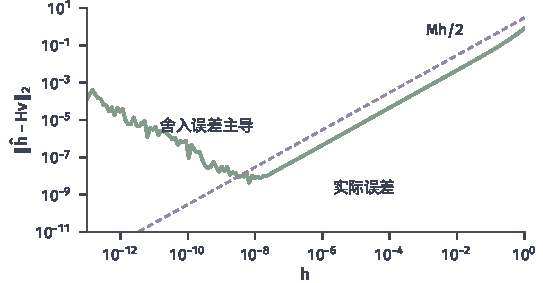
\includegraphics[width=92mm]{figures/05-optimization/02-smooth-optimization/matplotlib/saddle-hvp-difference/figure.pdf}
  \caption{目标~\eqref{eq:saddle-example}在点$(0.3,0.2)$沿$(1,1)/\sqrt2$的差分Hessian向量积误差，绿线是实际误差（双精度计算），紫色虚线是上界$Mh/2$，$M=6$。$h$小于约$10^{-8}$后舍入误差占主导。}
  \label{fig:saddle-hvp-difference}
\end{BookInlineFigure}

\paragraph{主要思想：把最小特征值变成最大特征值}
Hessian向量积最直接的用法是幂迭代：反复乘一个矩阵，向量会转向模最大的特征值所对应的方向。可是我们要的是最小特征值，而$\bm{H}$的最大模特征值可能是最大的正特征值。

解决办法是平移。设$\lVert\bm{H}\rVert_2\leq L$，令
\begin{equation}
 \bm{A}=L\bm{I}-\bm{H}.
 \label{eq:saddle-power-shift}
\end{equation}
$\bm{A}$的特征向量和$\bm{H}$相同，特征值是$a_i=L-\lambda_i\geq0$，最大的$a_1=L-\lambda_{\min}$恰好对应$\bm{H}$的最小特征值。于是对$\bm{A}$作幂迭代：
\begin{equation}
 \bm{v}^{(k+1)}=\frac{\bm{A}\bm{v}^{(k)}}{\lVert\bm{A}\bm{v}^{(k)}\rVert_2},\qquad k=0,1,\ldots
 \label{eq:saddle-power-iteration}
\end{equation}

每轮只用一次Hessian向量积。这里的上标$k$记检测内部的轮数，与外层的迭代$t$区分。把$\bm{v}^{(0)}$按特征向量展开成$\sum_ic_i\bm{q}_i$，$k$轮之后的方向正比于$\sum_ic_ia_i^k\bm{q}_i$，与$a_1$相比较小的分量按几何级数衰减。

这个迭代还有另一层含义。除以$L$之后，$\bm{A}/L=\bm{I}-\tfrac1L\bm{H}$，这正是步长$1/L$的梯度下降在二次目标上的迭代矩阵。所以幂迭代和鞍点附近的梯度下降是同一件事，第~\ref{sec:saddle-escape}节还要用到这一点。

\needspace{6\baselineskip}
\paragraph{变量}
在一个给定的点上运行检测，要维护的量是：
\begin{itemize}
 \item $\bm{v}^{(k)}\in\mathbb{R}^n$：当前的单位向量；
 \item $\bm{u}^{(k)}\in\mathbb{R}^n$：Hessian向量积$\bm{H}\bm{v}^{(k)}$；
 \item $R^{(k)}$：Rayleigh商$\langle\bm{v}^{(k)},\bm{u}^{(k)}\rangle$。
\end{itemize}

\paragraph{初始化}
选定常数$L\geq\lVert\bm{H}\rVert_2$，阈值$\gamma>0$，轮数上限$k_{\max}$，并在单位球面上均匀随机地取$\bm{v}^{(0)}$。例中在原点检测，$\bm{H}=\operatorname{diag}(-1,1)$，$L=2$，$\gamma=\tfrac12$，设随机抽到
\[
 \bm{v}^{(0)}=\frac{1}{\sqrt2}\begin{bmatrix}1\\1\end{bmatrix}.
\]

\paragraph{每轮更新}
第$k$轮依次执行以下步骤，满足结束条件时停止。

\begin{enumerate}
 \item 计算Hessian向量积$\bm{u}^{(k)}=\bm{H}\bm{v}^{(k)}$。例中第$0$轮得到
 \[
  \bm{u}^{(0)}=\frac{1}{\sqrt2}\begin{bmatrix}-1\\1\end{bmatrix}.
 \]
 \item 计算$R^{(k)}$。若$R^{(k)}\leq-\gamma$，返回$\bm{v}^{(k)}$，宣布找到了负曲率方向；若$k=k_{\max}$，宣布没有找到。例中第$0$轮$R^{(0)}=0>-\tfrac12$，继续。
 \item 由式~\eqref{eq:saddle-power-shift}、\eqref{eq:saddle-power-iteration}计算新方向，$\bm{A}\bm{v}^{(k)}=L\bm{v}^{(k)}-\bm{u}^{(k)}$不需要再乘一次$\bm{H}$。例中第$0$轮
 \[
  L\bm{v}^{(0)}-\bm{u}^{(0)}=\frac{1}{\sqrt2}\begin{bmatrix}3\\1\end{bmatrix},\qquad
  \bm{v}^{(1)}=\frac{1}{\sqrt{10}}\begin{bmatrix}3\\1\end{bmatrix}.
 \]
\end{enumerate}

第$1$轮计算得
\[
 \bm{u}^{(1)}=\frac{1}{\sqrt{10}}\begin{bmatrix}-3\\1\end{bmatrix},\qquad
 R^{(1)}=\frac{-9+1}{10}=-0.8\leq-\frac12.
\]
于是结束，最终得到$\bm{v}=(3,1)/\sqrt{10}$，它不是特征向量，曲率$-0.8$却已经达到要求，整个过程用了$2$次Hessian向量积。

\paragraph{起点为什么要随机}
上面的计算依赖起点在$\bm{q}_1$上有分量。若起点恰好是$\bm{v}^{(0)}=(0,1)$，第一个分量永远是零，迭代留在原地，Rayleigh商永远是$+1$，算法会错误地宣布没有负曲率。

起点在$\bm{q}_1$上的分量小，要花的轮数就多。取$\bm{v}^{(0)}=(s,\sqrt{1-s^2})$，$k$轮后两分量之比放大到$3^ks/\sqrt{1-s^2}$，要让它达到$1$量级需要$k\approx\log_3(1/s)$轮。图~\ref{fig:saddle-krylov-blind}中曲线的拐点正随$s$变小而右移。这说明随机化换来的是“几乎不可能恰好落在坏的起点”，并且只需要付出对数代价。

\begin{BookInlineFigure}
  \centering
  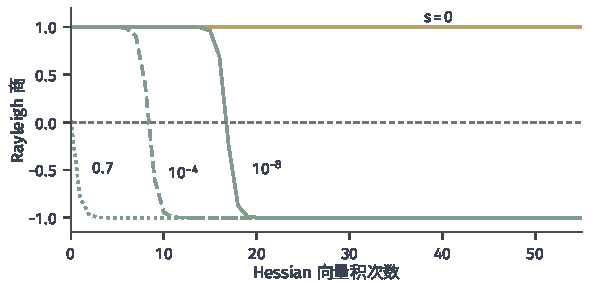
\includegraphics[width=100mm]{figures/05-optimization/02-smooth-optimization/matplotlib/saddle-krylov-blind/figure.pdf}
  \caption{$\bm{H}=\operatorname{diag}(-1,1)$，$L=2$，幂迭代的Rayleigh商随乘积次数的变化，起点是$(s,\sqrt{1-s^2})$。黄线$s=0$永远是$+1$，绿线从左到右$s=0.7,10^{-4},10^{-8}$，拐点依次右移，负曲率最终都被发现。}
  \label{fig:saddle-krylov-blind}
\end{BookInlineFigure}

\paragraph{找到和没有找到，结论不一样}
检测结束有两种结果，它们的可信程度差别很大。若$R^{(k)}\leq-\gamma$，这是一个算出来的事实：$\bm{v}$确实是曲率不超过$-\gamma$的方向，与随机抽样的运气无关。

若没有找到，结论就只能是概率性的。$\bm{v}^{(0)}$可能运气很差，迭代还没转过来就结束了。下面的定理说明，轮数足够多时，这种情况发生的概率很小。图~\ref{fig:saddle-detect-decision}概括了两种结论的区别。

\begin{BookInlineFigure}
  \centering
  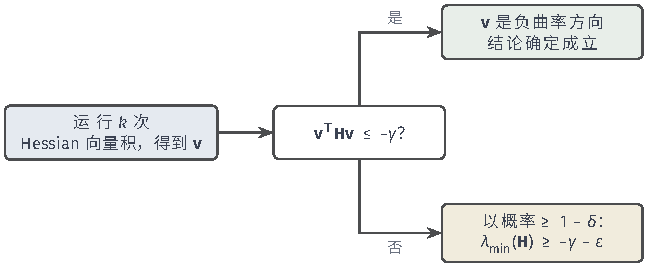
\includegraphics[width=109.6mm]{figures/05-optimization/02-smooth-optimization/tikz/saddle-detect-decision/figure.pdf}
  \caption{负曲率检测的两种结果。使用精确的Hessian向量积时，“找到”给出确定的结论；“未找到”只在随机起点成功的事件上成立，失败概率由$\delta$控制，$\varepsilon$是检测精度。}
  \label{fig:saddle-detect-decision}
\end{BookInlineFigure}

\begin{theorem}[幂迭代的概率保证]
 \label{thm:saddle-power}
 设$\bm{H}\in\mathbb{R}^{n\times n}$对称，$\lVert\bm{H}\rVert_2\leq L$，$\varepsilon\in(0,L]$，$\delta\in(0,1)$。$\bm{v}^{(0)}$在单位球面上均匀分布，幂迭代~\eqref{eq:saddle-power-iteration}运行$k$轮，其中
 \begin{equation}
  k\geq\frac{2L}{\varepsilon}\ln\frac{64Ln}{\pi\varepsilon\delta^3}.
  \label{eq:saddle-power-rounds}
 \end{equation}
 则至少以$1-\delta$的概率，
 \begin{equation}
  \bm{v}^{(k)\top}\bm{H}\bm{v}^{(k)}\leq\lambda_{\min}(\bm{H})+\varepsilon.
  \label{eq:saddle-power-guarantee}
 \end{equation}
\end{theorem}

\begin{proof}
 证明分两步：先说明随机起点在$\bm{q}_1$上的分量不会太小，再说明幂迭代把其余误差压下去。

 第一步处理起点。球面上的均匀分布可以写成$\bm{v}^{(0)}=\bm{z}/\lVert\bm{z}\rVert_2$，其中$\bm{z}$是标准正态向量。由旋转不变性，可以设$c_1=z_1/\lVert\bm{z}\rVert_2$是$\bm{v}^{(0)}$在$\bm{q}_1$上的分量。标准正态密度不超过$1/\sqrt{2\pi}$，所以
 \[
  \mathbb{P}\bigl(\lvert z_1\rvert\leq\tau\bigr)\leq\tau\sqrt{\frac{2}{\pi}}.
 \]

 取$\tau=\tfrac{\delta}{2}\sqrt{\pi/2}$，这个概率不超过$\delta/2$。又因为$\mathbb{E}\lVert\bm{z}\rVert_2^2=n$，由Markov不等式，
 \[
  \mathbb{P}\Bigl(\lVert\bm{z}\rVert_2^2>\frac{2n}{\delta}\Bigr)\leq\frac{\delta}{2}.
 \]

 因此至少以$1-\delta$的概率，两个事件都不发生，此时
 \[
  c_1^2\geq\frac{\tau^2}{2n/\delta}=\frac{\pi\delta^3}{16n}.
 \]

 第二步在这个事件上估计误差。记$a_i=L-\lambda_i$，$a_1$最大且$0\leq a_i\leq2L$；若$a_1=0$，$\bm{H}=L\bm{I}$，结论自动成立，下面设$a_1>0$。$\bm{v}^{(k)}$正比于$\bm{A}^k\bm{v}^{(0)}$，所以由$\bm{v}^\top\bm{H}\bm{v}=L-\bm{v}^\top\bm{A}\bm{v}$，
 \[
  \bm{v}^{(k)\top}\bm{H}\bm{v}^{(k)}-\lambda_{\min}
  =\frac{\sum_ic_i^2a_i^{2k}(a_1-a_i)}{\sum_ic_i^2a_i^{2k}}.
 \]

 把下标分成两组：$a_i\geq a_1-\varepsilon/2$的一组，分子中的因子$a_1-a_i$不超过$\varepsilon/2$，这一组对比值的贡献不超过$\varepsilon/2$。

 其余的下标满足$a_i<a_1-\varepsilon/2$，于是
 \[
  a_i^{2k}\leq a_1^{2k}\Bigl(1-\frac{\varepsilon}{2a_1}\Bigr)^{2k}
  \leq a_1^{2k}\exp\Bigl(-\frac{k\varepsilon}{a_1}\Bigr).
 \]

 分母至少是$c_1^2a_1^{2k}$，$a_1-a_i\leq a_1\leq2L$，$\sum_ic_i^2=1$，$a_1\leq2L$使指数不小于$k\varepsilon/(2L)$。所以这一组的贡献不超过
 \[
  \frac{2L}{c_1^2}\exp\Bigl(-\frac{k\varepsilon}{2L}\Bigr).
 \]

 代入$c_1^2$的下界和条件~\eqref{eq:saddle-power-rounds}，这个量不超过$\varepsilon/2$。两组相加，即得式~\eqref{eq:saddle-power-guarantee}。
\end{proof}

定理中各个量的作用可以逐项核对。$L/\varepsilon$来自幂迭代的收敛速度，要分辨相差$\varepsilon$的特征值，需要的轮数与$L/\varepsilon$成正比。$\ln n$和$\ln(1/\delta)$只出现在对数里，它们是随机起点要付的代价。

结论的含义是：运行满轮数仍然没有发现$R\leq-\gamma$时，以至少$1-\delta$的概率，
\begin{equation}
 \lambda_{\min}(\bm{H})\geq R^{(k)}-\varepsilon>-\gamma-\varepsilon.
 \label{eq:saddle-no-find}
\end{equation}

例中取$L=2$，$n=2$，$\varepsilon=\tfrac14$，$\delta=0.1$，式~\eqref{eq:saddle-power-rounds}要求$k\geq204$。上面的手算只用$2$次乘积就找到了方向。两者不矛盾：定理针对的是任意$\bm{H}$和最坏情形的起点分量，它要保证的是“没有找到”这个结论也能成立。

\paragraph{Lanczos方法}
幂迭代每轮只用最后一个向量，把前面的乘积结果都丢弃了。Lanczos方法保留整个Krylov子空间
\[
 \mathcal{K}_k=\operatorname{span}\bigl\{\bm{v}^{(0)},\bm{H}\bm{v}^{(0)},\ldots,\bm{H}^{k-1}\bm{v}^{(0)}\bigr\},
\]
并在这个子空间上取Rayleigh商的最小值。乘积次数相同，幂迭代的结果也落在同一个子空间内，所以Lanczos给出的值不会更差。它的三项递推和实现细节可参考\BookChapterRef{chap:krylov-methods}{卷二第15章“Krylov子空间法”}，这里只用它的结果：标准正交基下$\bm{H}$的投影是三对角矩阵$\bm{T}_k$，$\bm{T}_k$的最小特征值就是这个子空间上的最小Rayleigh商。

下面用一个三阶矩阵比较两者，它是在例子的Hessian上补一个中间特征值得到的：
\[
 \bm{H}=\operatorname{diag}(-1,1,2),\qquad
 \bm{v}^{(0)}=\frac{1}{\sqrt3}(1,1,1)^\top.
\]

第一步的对角元和残差是
\[
 \alpha_1=\frac23,\qquad
 \bm{w}=\bm{H}\bm{v}^{(0)}-\alpha_1\bm{v}^{(0)}
 =\frac{1}{3\sqrt3}\begin{bmatrix}-5\\1\\4\end{bmatrix},\qquad
 \beta_1=\lVert\bm{w}\rVert_2=\frac{\sqrt{14}}{3}.
\]

第二个基向量是$\bm{w}/\beta_1$，由此计算第二个对角元，得到
\[
 \alpha_2=\frac{-25+1+32}{42}=\frac{4}{21},\qquad
 \bm{T}_2=\begin{bmatrix}2/3&\sqrt{14}/3\\\sqrt{14}/3&4/21\end{bmatrix}.
\]

$\bm{T}_2$的最小特征值约为$-0.841$。同样用$2$次乘积，$L=2$的幂迭代$\bm{v}^{(1)}\propto(3,1,0)$给出$-0.8$。差距在小矩阵上不明显，在谱分布更不利时就很大了。

图~\ref{fig:saddle-power-lanczos}是一个$n=400$的例子。第二小的特征值紧贴最小特征值时，幂迭代几乎停滞，Lanczos仍然很快。原因是$k$次乘积相当于选一个$k$次多项式去放大$\bm{q}_1$分量，幂迭代固定用$a^k$，Lanczos等于在所有$k$次多项式中选最好的一个。

\begin{BookInlineFigure}
  \centering
  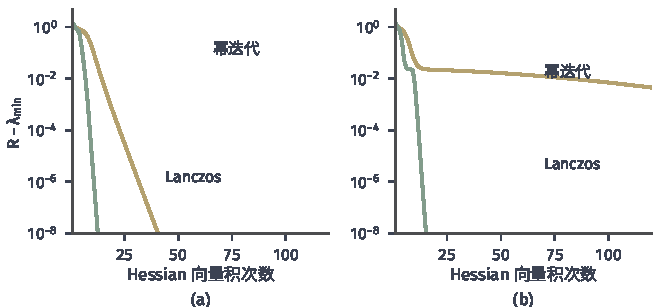
\includegraphics[width=112mm]{figures/05-optimization/02-smooth-optimization/matplotlib/saddle-power-lanczos/figure.pdf}
  \caption{同一个随机起点下幂迭代（黄，$L=2$）与Lanczos方法（绿）的Rayleigh商误差，$n=400$，$\lambda_{\min}=-0.2$，其余特征值在$[0.5,2]$上均匀取样，只有第二小的特征值另行指定。(a)第二小特征值为$0.3$。(b)第二小特征值为$-0.17$，与最小特征值很接近。}
  \label{fig:saddle-power-lanczos}
\end{BookInlineFigure}

定量结果是：均匀随机起点的Lanczos方法运行约$\sqrt{L/\varepsilon}\,\ln(n/\delta^2)$次乘积，就以至少$1-\delta$的概率达到精度$\varepsilon$。与定理~\ref{thm:saddle-power}相比，$L/\varepsilon$换成了它的平方根。证明需要用到Chebyshev多项式在区间外的增长估计，篇幅较长，读者可查阅数值线性代数的专门著作，这里只把它作为不加证明的事实使用。

Lanczos的计算也有代价：要存基向量才能算出方向，三项递推在有限精度下会失去正交性，运行次数多时需要重新正交化或重启。

\paragraph{误差怎样记入}
前面的结论默认Hessian向量积是精确的，用差分时要补上式~\eqref{eq:saddle-hvp-error}。对“找到”这一方，算出的$\hat{R}=\bm{v}^\top\hat{\bm{u}}$与真实Rayleigh商至多相差$Mh/2$，把判定条件改成$\hat{R}\leq-\gamma-Mh/2$，就能确定地推出$R(\bm{v})\leq-\gamma$。

对“没有找到”这一方，差分误差还会改变迭代本身，定理~\ref{thm:saddle-power}不能直接套用，分析时必须把每一轮的乘积误差累加进去。实际程序里，要做这一判断时通常用自动微分得到精确的乘积。表~\ref{tab:saddle-detect-compare}总结了几种方式。

\begin{BookInlineTable}
  \centering
  \begin{tabular}{@{}llll@{}}
    \toprule
    检测方式 & 成本 & 找到时 & 未找到时\\
    \midrule
    特征分解 & $O(n^3)$ & 确定 & 确定\\
    Cholesky试探 & $O(n^3)$，只判断 & 确定 & 确定\\
    幂迭代 & $O(\frac{L}{\varepsilon}\ln\frac{n}{\delta})$次乘积 & 确定 & $\geq1-\delta$\\
    Lanczos & $O(\sqrt{\frac{L}{\varepsilon}}\ln\frac{n}{\delta})$次乘积 & 确定 & $\geq1-\delta$\\
    差分乘积 & 每次两个梯度 & 加余量$Mh/2$ & 累加误差\\
    \bottomrule
  \end{tabular}
  \caption{负曲率检测方式的比较，“确定”不计舍入误差，“$\geq1-\delta$”指结论成立的概率。$O(\cdot)$中省略了$L/\varepsilon$的对数因子。}
  \label{tab:saddle-detect-compare}
\end{BookInlineTable}


\section{离开鞍点}
\label{sec:saddle-escape}

迭代点已经到了梯度很小的鞍点邻域，怎样离开？回答取决于手里有什么信息。知道一个负曲率方向时，可以沿它走一步；只有梯度时，可以给迭代点一点随机扰动，让梯度下降自己放大不稳定的分量；有二次模型时，可以保留模型的不定性，让子问题自己走到负曲率的一侧。三种机制各有条件，都不能把严格鞍点的结论直接搬到退化驻点上。

\subsection{负曲率步}
\label{sec:saddle-nc-step}

上一节的检测给出了单位向量$\bm{v}$，满足$\bm{v}^\top\bm{H}\bm{v}\leq-\gamma$。站在山口上，这是一条明确的下坡路。问题是这样走一步能保证下降多少，步长又该取多大。

\paragraph{为什么要控制Hessian的变化}
二阶模型沿$\bm{v}$的预测是$-\tfrac12\gamma\alpha^2$，步长越大下降越多，但这个预测不可能一直成立。模型只在局部有效，走远了Hessian会变。例中沿$x_1$轴，
\[
 f(\alpha,0)=\frac14\bigl(\alpha^2-1\bigr)^2.
\]

$\alpha=1$处到达谷底，$\alpha=\sqrt2$处函数值回到$1/4$，再往前目标反而高于起点。所以负曲率方向不能无限延长，步长要受Hessian变化速度的约束，这个速度就是$M$。下面的引理给出二阶模型的误差。

\begin{lemma}[三次上界]
 \label{lem:saddle-cubic}
 设$\nabla^2f$在凸集$\bm{U}$上是$M$-Lipschitz的，$\bm{x}$与$\bm{x}+\bm{p}$都在$\bm{U}$中。记$\bm{g}=\nabla f(\bm{x})$，$\bm{H}=\nabla^2f(\bm{x})$，则
 \begin{equation}
  \Bigl\lvert f(\bm{x}+\bm{p})-f(\bm{x})-\langle\bm{g},\bm{p}\rangle-\frac12\bm{p}^\top\bm{H}\bm{p}\Bigr\rvert
  \leq\frac{M}{6}\lVert\bm{p}\rVert_2^3.
  \label{eq:saddle-cubic}
 \end{equation}
\end{lemma}

\begin{proof}
 令$\phi(s)=f(\bm{x}+s\bm{p})$，$s\in[0,1]$。由积分余项形式的Taylor公式，
 \[
  \phi(1)=\phi(0)+\phi'(0)+\int_0^1(1-s)\phi''(s)\,\mathrm{d}s.
 \]

 其中$\phi'(0)=\langle\bm{g},\bm{p}\rangle$。又因为$\int_0^1(1-s)\,\mathrm{d}s=\tfrac12$，二次项可以写进同一个积分，得到
 \[
  f(\bm{x}+\bm{p})-f(\bm{x})-\langle\bm{g},\bm{p}\rangle-\frac12\bm{p}^\top\bm{H}\bm{p}
  =\int_0^1(1-s)\bigl(\phi''(s)-\phi''(0)\bigr)\,\mathrm{d}s.
 \]

 $\phi$的二阶导数是Hessian沿$\bm{p}$的二次型，由Lipschitz条件，
 \[
  \lvert\phi''(s)-\phi''(0)\rvert
  =\bigl\lvert\bm{p}^\top\bigl(\nabla^2f(\bm{x}+s\bm{p})-\bm{H}\bigr)\bm{p}\bigr\rvert
  \leq Ms\lVert\bm{p}\rVert_2^3.
 \]

 代入并用$\int_0^1(1-s)s\,\mathrm{d}s=\tfrac16$，即得式~\eqref{eq:saddle-cubic}。
\end{proof}

\paragraph{选符号，定步长}
梯度不为零时，$\bm{v}$和$-\bm{v}$的曲率相同，一阶项却相反。所以先选符号，使一阶项不起反作用。下面的定理给出一步的下降量。

\begin{theorem}[负曲率步的下降]
 \label{thm:saddle-nc-step}
 设单位向量$\bm{v}$满足$\bm{v}^\top\bm{H}\bm{v}\leq-\gamma<0$和$\langle\bm{g},\bm{v}\rangle\leq0$，引理~\ref{lem:saddle-cubic}的条件对$\bm{p}=\alpha\bm{v}$成立。则对$\alpha>0$，
 \begin{equation}
  f(\bm{x}+\alpha\bm{v})\leq f(\bm{x})-\frac{\gamma}{2}\alpha^2+\frac{M}{6}\alpha^3.
  \label{eq:saddle-nc-bound}
 \end{equation}
 取$\alpha=2\gamma/M$时，
 \begin{equation}
  f(\bm{x}+\alpha\bm{v})\leq f(\bm{x})-\frac{2\gamma^3}{3M^2}.
  \label{eq:saddle-nc-decrease}
 \end{equation}
\end{theorem}

\begin{proof}
 由式~\eqref{eq:saddle-cubic}取$\bm{p}=\alpha\bm{v}$，$\lVert\bm{p}\rVert_2=\alpha$，得到
 \[
  f(\bm{x}+\alpha\bm{v})\leq f(\bm{x})+\alpha\langle\bm{g},\bm{v}\rangle+\frac{\alpha^2}{2}\bm{v}^\top\bm{H}\bm{v}+\frac{M}{6}\alpha^3.
 \]

 由$\langle\bm{g},\bm{v}\rangle\leq0$和$\bm{v}^\top\bm{H}\bm{v}\leq-\gamma$，即得式~\eqref{eq:saddle-nc-bound}。右端作为$\alpha$的函数，对$\alpha$求导得$-\gamma\alpha+\tfrac12M\alpha^2$，在$\alpha=2\gamma/M$处取到最小。代入得
 \[
  -\frac{\gamma}{2}\cdot\frac{4\gamma^2}{M^2}+\frac{M}{6}\cdot\frac{8\gamma^3}{M^3}
  =-\frac{2\gamma^3}{M^2}+\frac{4\gamma^3}{3M^2}
  =-\frac{2\gamma^3}{3M^2}.
 \]
\end{proof}

下降量只依赖负曲率的大小和Hessian的变化速度，与梯度多小无关。这正是它补上梯度步短板的地方：梯度步的保证是$\lVert\bm{g}\rVert_2^2/(2L)$，鞍点附近这个量几乎为零。

例中在原点取$\bm{v}=(1,0)$，$\gamma=1$，$M=6$，步长$\alpha=1/3$。定理保证的下降是
\[
 \frac{2\gamma^3}{3M^2}=\frac{1}{54}\approx0.0185.
\]
实际下降是
\[
 f(\bm{0})-f\bigl(\tfrac13,0\bigr)=\frac14-\frac{16}{81}\approx0.0525.
\]
图~\ref{fig:saddle-nc-slice}(a)沿$x_1$轴比较目标（蓝）、二次模型（绿）和三次上界（紫）。三次上界在$\bm{U}$内从上方盖住目标，绿点$\alpha=1/3$是上界的最低点，这个步长比实际的最好步长$\alpha=1$保守得多。

\begin{BookInlineFigure}
  \centering
  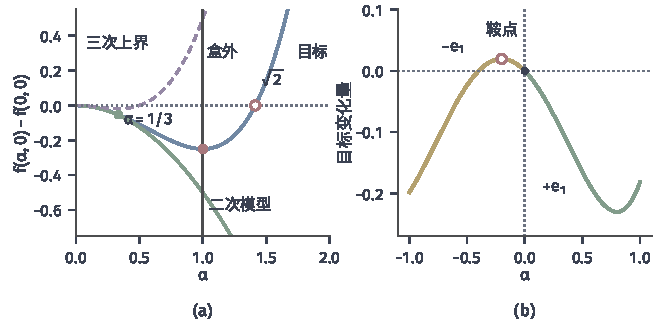
\includegraphics[width=112mm]{figures/05-optimization/02-smooth-optimization/matplotlib/saddle-nc-slice/figure.pdf}
  \caption{沿负曲率方向的一维截面。(a)原点沿$\bm{e}_1$：蓝线是目标减去$f(\bm{0})$，绿线是二次模型$-\alpha^2/2$，紫色虚线是三次上界$-\alpha^2/2+\alpha^3$，竖线是带形$\bm{U}$的边界。空心点$\alpha=\sqrt2$处目标回到起点的值。(b)从$(0.2,0)$出发沿$\pm\bm{e}_1$的目标变化，此处$\langle\bm{g},\bm{e}_1\rangle<0$。绿线一开始就下降，黄线先升到鞍点的高度才下降。}
  \label{fig:saddle-nc-slice}
\end{BookInlineFigure}

符号的作用见图~\ref{fig:saddle-nc-slice}(b)。在$(0.2,0)$处，梯度的第一个分量是$0.008-0.2=-0.192$，$+\bm{e}_1$满足$\langle\bm{g},\bm{v}\rangle<0$。朝$-\bm{e}_1$走，目标要先爬回鞍点才开始下降，一阶项抵消了曲率的好处。

\paragraph{不知道$M$时}
步长$2\gamma/M$要用到$M$，多数问题不知道它的值。这时可以回溯：从$\alpha_0$开始，不断折半，直到满足
\begin{equation}
 f(\bm{x}+\alpha\bm{v})\leq f(\bm{x})-\frac{\gamma}{4}\alpha^2.
 \label{eq:saddle-nc-backtrack}
\end{equation}

由式~\eqref{eq:saddle-nc-bound}，条件成立只需要
\[
 -\frac12\gamma\alpha^2+\frac16M\alpha^3\leq-\frac14\gamma\alpha^2,
\]
也就是$\alpha\leq3\gamma/(2M)$。折半回溯接受的步长因此不小于$\min\{\alpha_0,3\gamma/(4M)\}$，当$\alpha_0$足够大时，一步的下降不少于
\[
 \frac{\gamma}{4}\Bigl(\frac{3\gamma}{4M}\Bigr)^2=\frac{9\gamma^3}{64M^2}.
\]
例中取$\alpha_0=2$，$f(2,0)=9/4$被拒绝，$\alpha=1$时$f(1,0)=0\leq\tfrac14-\tfrac14$，被接受，一步到达谷底。

\paragraph{主要思想：梯度步和负曲率步交替}
梯度步在梯度大时有效，负曲率步在梯度小时仍然有效，两者正好互补。算法每轮先看梯度：梯度大就走梯度步；梯度小才花力气检测负曲率；两者都不能下降就停止。写成公式，
\begin{equation}
 \bm{x}^{(t+1)}=
 \begin{cases}
  \bm{x}^{(t)}-\dfrac{1}{L}\bm{g}^{(t)}, & \lVert\bm{g}^{(t)}\rVert_2>\varepsilon_g,\\
  \bm{x}^{(t)}+\dfrac{2\gamma^{(t)}}{M}\bm{v}^{(t)}, & \text{其他情形且检测到负曲率}.
 \end{cases}
 \label{eq:saddle-nc-update}
\end{equation}
其中单位向量$\bm{v}^{(t)}$的曲率是$-\gamma^{(t)}$，符号已经选定。$\varepsilon_g$和$\varepsilon_H$是梯度和曲率的容差，第~\ref{sec:saddle-stopping}节再讨论怎样取值。

\needspace{6\baselineskip}
\paragraph{变量}
算法要维护的量是：
\begin{itemize}
 \item $\bm{x}^{(t)}\in\mathbb{R}^n$：当前点；
 \item $\bm{g}^{(t)}\in\mathbb{R}^n$：当前梯度，每轮读取一次；
 \item $\bm{v}^{(t)}\in\mathbb{R}^n$，$\gamma^{(t)}>0$：只在梯度小的轮次计算的负曲率方向及其大小。
\end{itemize}

\paragraph{初始化}
选定$\bm{x}^{(0)}$、$L$、$M$和容差。例中$L=2$，$M=6$，$\varepsilon_g=0.1$，$\varepsilon_H=\sqrt{M\varepsilon_g}\approx0.775$，起点取在$x_2$轴上，并且用特征分解做检测：
\[
 \bm{x}^{(0)}=\begin{bmatrix}0\\1\end{bmatrix}.
\]

\paragraph{每轮更新}
第$t$轮依次执行以下步骤，直到第$3$步宣布停止。

\begin{enumerate}
 \item 计算$\bm{g}^{(t)}$。若$\lVert\bm{g}^{(t)}\rVert_2>\varepsilon_g$，由式~\eqref{eq:saddle-nc-update}走梯度步，进入下一轮。例中前$4$轮$x_1$一直是$0$，$x_2$每轮减半：
 \[
  \bm{x}^{(1)}=\begin{bmatrix}0\\0.5\end{bmatrix},\quad
  \bm{x}^{(2)}=\begin{bmatrix}0\\0.25\end{bmatrix},\quad
  \bm{x}^{(3)}=\begin{bmatrix}0\\0.125\end{bmatrix},\quad
  \bm{x}^{(4)}=\begin{bmatrix}0\\0.0625\end{bmatrix}.
 \]
 \item 否则检测负曲率。例中第$4$轮$\lVert\bm{g}^{(4)}\rVert_2=0.0625\leq0.1$，由式~\eqref{eq:saddle-example-derivatives}，
 \[
  \bm{H}^{(4)}=\operatorname{diag}(-1,1),\qquad\lambda_{\min}=-1<-\varepsilon_H.
 \]
 \item 若$\lambda_{\min}\geq-\varepsilon_H$，停止并返回$\bm{x}^{(t)}$。否则取$\bm{v}^{(t)}$为最小特征向量，$\gamma^{(t)}=-\lambda_{\min}$，选好符号，由式~\eqref{eq:saddle-nc-update}走负曲率步。例中第$4$轮$\langle\bm{g}^{(4)},\bm{e}_1\rangle=0$，取$\bm{v}=\bm{e}_1$，步长$1/3$，得到
 \[
  \bm{x}^{(5)}=\begin{bmatrix}1/3\\0.0625\end{bmatrix}.
 \]
\end{enumerate}

此后梯度已经变大，算法回到梯度步。表~\ref{tab:saddle-nc-run}列出全过程。第$9$轮$\lVert\bm{g}^{(9)}\rVert_2=0.060\leq0.1$，Hessian是$\operatorname{diag}(1.815,1)$，$\lambda_{\min}=1\geq-\varepsilon_H$，算法停止，最终得到$\bm{x}^{(9)}\approx(0.9686,0.0039)$。

\begin{BookInlineTable}
  \centering
  \begin{tabular}{@{}rccccl@{}}
    \toprule
    $t$ & $\bm{x}^{(t)}$ & $f$ & $\lVert\bm{g}^{(t)}\rVert_2$ & $\lambda_{\min}$ & 本轮动作\\
    \midrule
    $0$ & $(0,\ 1)$ & $0.7500$ & $1.000$ & $-1$ & 梯度步\\
    $1$ & $(0,\ 0.5)$ & $0.3750$ & $0.500$ & $-1$ & 梯度步\\
    $2$ & $(0,\ 0.25)$ & $0.2813$ & $0.250$ & $-1$ & 梯度步\\
    $3$ & $(0,\ 0.125)$ & $0.2578$ & $0.125$ & $-1$ & 梯度步\\
    $4$ & $(0,\ 0.0625)$ & $0.2520$ & $0.063$ & $-1$ & 负曲率步\\
    $5$ & $(0.3333,\ 0.0625)$ & $0.1995$ & $0.303$ & $-0.667$ & 梯度步\\
    $6$ & $(0.4815,\ 0.0313)$ & $0.1480$ & $0.371$ & $-0.305$ & 梯度步\\
    $7$ & $(0.6664,\ 0.0156)$ & $0.0774$ & $0.371$ & $0.332$ & 梯度步\\
    $8$ & $(0.8516,\ 0.0078)$ & $0.0189$ & $0.234$ & $1$ & 梯度步\\
    $9$ & $(0.9686,\ 0.0039)$ & $0.0010$ & $0.060$ & $1$ & 停止\\
    \bottomrule
  \end{tabular}
  \caption{梯度步与负曲率步在目标~\eqref{eq:saddle-example}上的运行。$\varepsilon_g=0.1$，$\varepsilon_H\approx0.775$，$\lambda_{\min}$是Hessian~\eqref{eq:saddle-example-derivatives}的最小特征值，第$8$、$9$轮第一个对角元已大于$1$，最小特征值取到$1$。}
  \label{tab:saddle-nc-run}
\end{BookInlineTable}

图~\ref{fig:saddle-nc-run}对照了不做检测的梯度下降。两者前$4$轮完全相同；梯度下降从此沿$x_2$轴收敛到鞍点，目标停在$1/4$，而负曲率步使迭代点离开了这条轴。

\begin{BookInlineFigure}
  \centering
  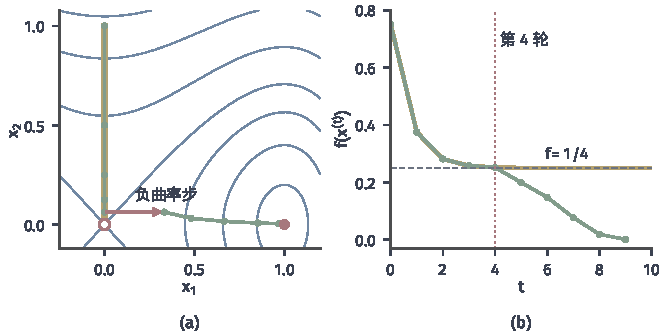
\includegraphics[width=112mm]{figures/05-optimization/02-smooth-optimization/matplotlib/saddle-nc-run/figure.pdf}
  \caption{从$(0,1)$出发的运行，步长$\alpha=1/2$。(a)绿色折线是梯度步与负曲率步的路径，红色箭头是第$4$轮的负曲率步，黄线（被绿线部分遮挡）是梯度下降，沿$x_2$轴收敛到空心点所示的鞍点。(b)目标值随轮数的变化，黄线趋于虚线$f=1/4$，绿线在红色点线所示的第$4$轮之后继续下降。}
  \label{fig:saddle-nc-run}
\end{BookInlineFigure}

\paragraph{算法分析}
每轮的下降都有下界，累加就得到轮数上界，论证与第~\ref{chap:smooth-foundations}章的累加下降相同。下面的定理把检测精度写成一个参数，以便同时覆盖精确和近似检测。

\begin{theorem}[交替算法的轮数]
 \label{thm:saddle-nc-count}
 设$f$有下界$f_{\inf}$，$\nabla f$和$\nabla^2f$在包含各步线段的凸集上分别是$L$-Lipschitz和$M$-Lipschitz的。设每次走负曲率步时都有$\gamma^{(t)}\geq\gamma_0>0$，记$\Delta_f=f(\bm{x}^{(0)})-f_{\inf}$。则算法~\eqref{eq:saddle-nc-update}停止之前的轮数$T$满足
 \begin{equation}
  T\leq\Delta_f\max\Bigl\{\frac{2L}{\varepsilon_g^2},\ \frac{3M^2}{2\gamma_0^3}\Bigr\}.
  \label{eq:saddle-nc-count}
 \end{equation}
\end{theorem}

\begin{proof}
 由下降引理，走梯度步的轮次下降至少$\lVert\bm{g}^{(t)}\rVert_2^2/(2L)$，而这些轮次$\lVert\bm{g}^{(t)}\rVert_2>\varepsilon_g$，下降超过$\varepsilon_g^2/(2L)$。

 由定理~\ref{thm:saddle-nc-step}，走负曲率步的轮次下降至少$2\gamma_0^3/(3M^2)$。记两者中较小的为$c$，累加$T$轮得
 \[
  \Delta_f\geq f(\bm{x}^{(0)})-f(\bm{x}^{(T)})\geq Tc.
 \]
 除以$c$即得式~\eqref{eq:saddle-nc-count}。
\end{proof}

例中$\Delta_f=3/4$。精确检测对应$\gamma_0=\varepsilon_H$，两项分别是$400$和约$116$，上界是$300$轮，实际只用了$9$轮。这也是一个最坏情形的界，它只用到$L$、$M$、$\Delta_f$，没有用到例子的具体形状。

\paragraph{适用范围}
这个算法要求能算出负曲率方向，在第~\ref{sec:saddle-detection}节的意义下，检测是确定的或者带失败概率的，第~\ref{sec:saddle-stopping}节再把这部分成本计入。定理只保证算法在有限步内停止，停止时的点满足两个容差，它不说明这个点是局部极小点。Hessian不是Lipschitz连续时，式~\eqref{eq:saddle-cubic}没有依据，步长公式也就失去了基础。

\subsection{扰动梯度法}
\label{sec:saddle-perturbed}

现在假设只能读取梯度，连Hessian向量积也不用。梯度下降在鞍点附近究竟怎样运动，是分析的起点。

\paragraph{鞍点附近的线性运动}
设$\bm{x}^\star$是严格鞍点，$\bm{H}=\nabla^2f(\bm{x}^\star)$。在$\bm{x}^\star$附近$\nabla f(\bm{x})\approx\bm{H}(\bm{x}-\bm{x}^\star)$，梯度下降近似于线性迭代：
\begin{equation}
 \bm{x}^{(t+1)}-\bm{x}^\star\approx(\bm{I}-\alpha\bm{H})\bigl(\bm{x}^{(t)}-\bm{x}^\star\bigr).
 \label{eq:saddle-linear}
\end{equation}

沿特征向量$\bm{q}_i$的分量每步乘以$1-\alpha\lambda_i$。$\alpha=1/L$时，正曲率方向的因子在$[0,1)$内，分量收缩；负曲率方向的因子$1+\alpha\lvert\lambda_i\rvert$大于$1$，分量放大。这正是第~\ref{sec:saddle-detection}节的幂迭代：梯度下降本身就在放大最负的方向。

例中两个坐标的迭代是
\[
 x_1^{(t+1)}=\frac32x_1^{(t)}-\frac12\bigl(x_1^{(t)}\bigr)^3,\qquad
 x_2^{(t+1)}=\frac12x_2^{(t)}.
\]
在原点附近，$x_1$每步约乘以$1.5$，$x_2$每步乘以$0.5$。图~\ref{fig:saddle-gd-linear}(b)的对数坐标下，两者都是直线，直到$x_1$接近$1$才不再增长。

\begin{BookInlineFigure}
  \centering
  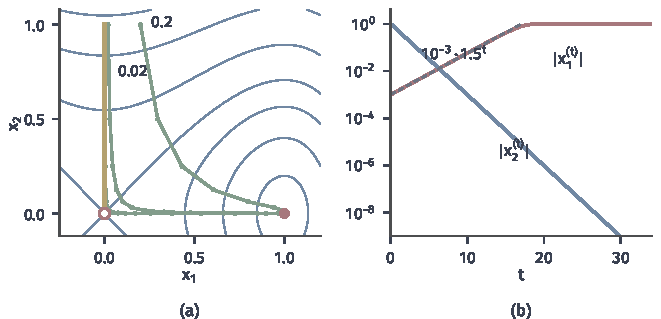
\includegraphics[width=112mm]{figures/05-optimization/02-smooth-optimization/matplotlib/saddle-gd-linear/figure.pdf}
  \caption{目标~\eqref{eq:saddle-example}上步长$1/2$的梯度下降。(a)从$(s,1)$出发的路径，绿线$s=0.2,0.02,0.002$，黄线$s=0$沿$x_2$轴收敛到鞍点。$s$越小，路径越贴近鞍点，徘徊越久。(b)从$(10^{-3},1)$出发，$\lvert x_1^{(t)}\rvert$（红）按$1.5^t$增长（灰色虚线），$\lvert x_2^{(t)}\rvert$（蓝）按$0.5^t$衰减。}
  \label{fig:saddle-gd-linear}
\end{BookInlineFigure}

\paragraph{什么样的初值会收敛到鞍点}
例中只要$x_1^{(0)}\neq0$，这个分量迟早被放大；只有$x_1^{(0)}=0$的点才一直留在$x_2$轴上，收敛到鞍点。这条轴是鞍点的\term{稳定流形}（stable manifold），二维平面上它的面积为零。

这个观察有严格的版本：设$f$二阶连续可微，$\nabla f$全局$L$-Lipschitz，步长$0<\alpha<1/L$，初值的分布对Lebesgue测度绝对连续，则梯度下降收敛到严格鞍点的概率为零\scite{lee2016gradient}。证明需要把迭代写成微分同胚，再用中心稳定流形定理，篇幅较长，读者可查阅原文。

这个结论有三个限度。第一，它的随机性只来自初值，之后的迭代完全确定。第二，它只排除收敛到严格鞍点，不说明会收敛到局部极小点，迭代也可能根本不收敛。第三，它是渐近的，没有说需要多少步。第三点不能靠更细的分析补上：要让$\lvert x_1\rvert$增长到$0.5$，例中的轮数如下。

\begin{BookInlineTable}
  \centering
  \begin{tabular}{@{}ccccc@{}}
    \toprule
    $x_1^{(0)}$ & $10^{-3}$ & $10^{-6}$ & $10^{-9}$ & $10^{-12}$\\
    \midrule
    轮数 & $16$ & $33$ & $50$ & $67$\\
    \bottomrule
  \end{tabular}
  \caption{目标~\eqref{eq:saddle-example}上$\lvert x_1^{(t)}\rvert$首次达到$0.5$所需的轮数。}
  \label{tab:saddle-escape-time}
\end{BookInlineTable}

初值的$x_1$可以任意接近零，轮数就可以任意大。所以普通梯度下降没有一个对所有初值都成立的有限步上界。要得到有限步的保证，必须让算法自己把迭代点推离稳定流形。

\paragraph{主要思想：只需要一点扰动}
图~\ref{fig:saddle-stuck-band}用数值实验看这件事。以原点为中心取半径$0.25$的圆盘，把每个点作为初值运行若干步梯度下降，再标出目标没有下降足够多的初值。这些“卡住”的初值组成一条沿$x_2$方向的窄带，步数越多，窄带越窄。

\begin{BookInlineFigure}
  \centering
  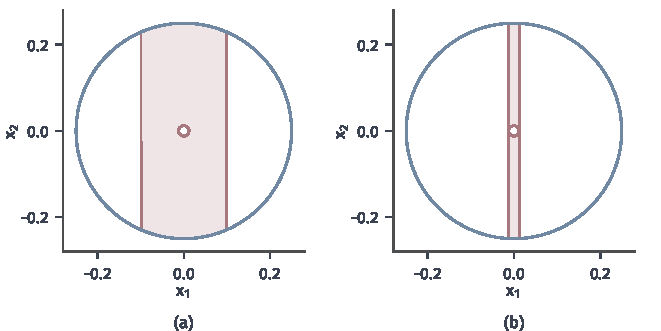
\includegraphics[width=112mm]{figures/05-optimization/02-smooth-optimization/matplotlib/saddle-stuck-band/figure.pdf}
  \caption{从半径$0.25$的圆盘（蓝线）内出发的梯度下降，步长$1/2$。红色窄带内的初值在$T$步后仍有$f>1/4-0.05$。(a)$T=3$，带的半宽约$0.099$。(b)$T=8$，带的半宽约$0.013$。窄带以外的点都已离开鞍点。}
  \label{fig:saddle-stuck-band}
\end{BookInlineFigure}

因此，在鞍点附近的小球内随机选一个点，落在窄带里的概率很小。图~\ref{fig:saddle-perturb-band}是概率的几何含义：窄带的体积与整个球的体积之比。只要球内的点几乎都能离开，加一点随机扰动就够了，扰动不需要很大。

\begin{BookInlineFigure}
  \centering
  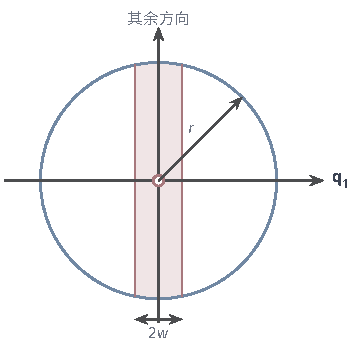
\includegraphics[width=61mm]{figures/05-optimization/02-smooth-optimization/tikz/saddle-perturb-band/figure.pdf}
  \caption{半径$r$的球内，沿$\bm{q}_1$方向半宽$w$的窄带。均匀随机的扰动落入窄带的概率就是两者的体积比。窄带外的点在$\bm{q}_1$上的分量至少是$w$。}
  \label{fig:saddle-perturb-band}
\end{BookInlineFigure}

先在二次目标上把这件事算清楚，此时$\bm{x}^\star$处的线性近似~\eqref{eq:saddle-linear}是精确的，全部论证都能写出来。

\begin{theorem}[二次目标上的逃离]
 \label{thm:saddle-quadratic-escape}
 设$f(\bm{x})=\tfrac12\bm{x}^\top\bm{H}\bm{x}$，$\bm{H}\in\mathbb{R}^{n\times n}$对称，$\lVert\bm{H}\rVert_2\leq L$，$\lambda_{\min}(\bm{H})=-\gamma<0$。$\bm{x}^{(0)}$在半径$r$的球内均匀分布，按步长$1/L$作梯度下降，迭代矩阵是$\bm{I}-\bm{H}/L$。给定$F>0$，$\delta\in(0,1)$，若
 \begin{equation}
  T\geq\frac{L}{\gamma}\ln\frac{4n\,(Lr^2+2F)}{\pi\gamma\,\delta^2r^2},
  \label{eq:saddle-quadratic-steps}
 \end{equation}
 则至少以$1-\delta$的概率，
 \begin{equation}
  f(\bm{x}^{(T)})\leq-F.
  \label{eq:saddle-quadratic-result}
 \end{equation}
\end{theorem}

\begin{proof}
 设$c_i=\langle\bm{x}^{(0)},\bm{q}_i\rangle$，$\bm{q}_1$对应$-\gamma$。证明分三步。

 第一步估计$c_1$不太小的概率。令$w>0$，事件$\lvert c_1\rvert\leq w$是球内半宽$w$的窄带，它的体积不超过宽度$2w$乘以$(n-1)$维截面的最大体积。记$V_m$为$m$维单位球的体积，于是
 \[
  \mathbb{P}\bigl(\lvert c_1\rvert\leq w\bigr)\leq\frac{2w\,r^{n-1}V_{n-1}}{r^nV_n}=\frac{2w}{r}\cdot\frac{V_{n-1}}{V_n}.
 \]

 单位球体积比由Gamma函数给出，再用Wendel不等式$\Gamma(x+\tfrac12)/\Gamma(x)\leq\sqrt{x}$，取$x=\tfrac{n+1}{2}$，得到
 \[
  \frac{V_{n-1}}{V_n}=\frac{\Gamma(\frac n2+1)}{\sqrt\pi\,\Gamma(\frac{n+1}{2})}\leq\sqrt{\frac{n+1}{2\pi}}\leq\sqrt{\frac{n}{\pi}}.
 \]

 取$w=\tfrac{r\delta}{2}\sqrt{\pi/n}$，窄带的概率不超过$\delta$。所以至少以$1-\delta$的概率，
 \[
  c_1^2\geq w^2=\frac{\pi\delta^2r^2}{4n}.
 \]

 第二步写出迭代的目标值。$\bm{x}^{(T)}$在$\bm{q}_i$上的分量是$(1-\lambda_i/L)^Tc_i$，所以
 \[
  f(\bm{x}^{(T)})=\frac12\sum_i\lambda_i\Bigl(1-\frac{\lambda_i}{L}\Bigr)^{2T}c_i^2.
 \]

 对$\lambda_i\geq0$的项，$0\leq1-\lambda_i/L\leq1$，这些项的和不超过$\tfrac12L\sum_ic_i^2\leq\tfrac12Lr^2$。对$\lambda_i<0$的项，它们都不大于零，只保留$\bm{q}_1$这一项，得到
 \[
  f(\bm{x}^{(T)})\leq\frac12Lr^2-\frac12\gamma\Bigl(1+\frac{\gamma}{L}\Bigr)^{2T}c_1^2.
 \]

 第三步确定步数。要使右端不超过$-F$，只需
 \[
  \Bigl(1+\frac{\gamma}{L}\Bigr)^{2T}\geq\frac{Lr^2+2F}{\gamma c_1^2}.
 \]

 由$\gamma\leq L$和不等式$\ln(1+y)\geq y/2$（$0\leq y\leq1$），左端的对数至少是$T\gamma/L$。代入$c_1^2$的下界，条件~\eqref{eq:saddle-quadratic-steps}恰好保证上式成立。
\end{proof}

定理把扰动的作用说清楚了。步数的主要部分是$L/\gamma$，即放大一倍需要的步数。维数$n$和失败概率$\delta$都在对数里，这是因为分量按指数增长，初值小一个倍数只增加常数步。高维时随机向量在任一方向上的分量约为$r/\sqrt n$，这个$\sqrt n$只通过$\ln n$进入步数。

例中在二次近似$\operatorname{diag}(-1,1)$上取$n=2$，$L=2$，$\gamma=1$，$r=0.05$，$F=0.05$，$\delta=0.1$，式~\eqref{eq:saddle-quadratic-steps}的右端约为$18.6$，所以$T=19$就够了。

图~\ref{fig:saddle-escape-scaling}用模拟检验定理。Hessian取$\operatorname{diag}(-\gamma,1,\ldots,1)$，其余参数同上，统计达到$f\leq-F$的步数。(a)中维数从$2$增加到$10^5$，中位数只从$7$增加到$20$。(b)中步数随$\gamma$减小按$1/\gamma$增长。上界比实际步数略大，但两种依赖关系都吻合。

\begin{BookInlineFigure}
  \centering
  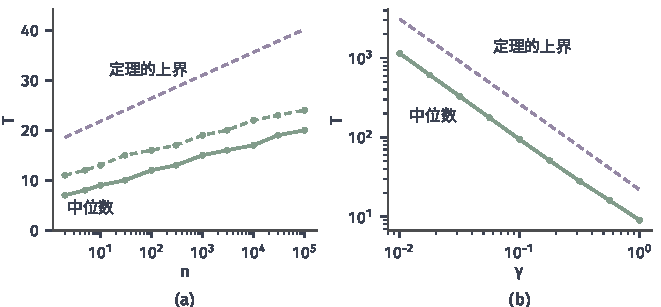
\includegraphics[width=112mm]{figures/05-optimization/02-smooth-optimization/matplotlib/saddle-escape-scaling/figure.pdf}
  \caption{二次目标上达到$f\leq-F$所需步数的模拟，每组$3000$次，$L=2$，$r=0.05$，$F=0.05$，Hessian取$\operatorname{diag}(-\gamma,1,\ldots,1)$。绿色实线是中位数，绿色虚线是$90\%$分位数，紫色虚线是式~\eqref{eq:saddle-quadratic-steps}在$\delta=0.1$时的上界。(a)$\gamma=1$，步数随维数$n$对数增长。(b)$n=10$，步数约与$1/\gamma$成正比。}
  \label{fig:saddle-escape-scaling}
\end{BookInlineFigure}

把上面的想法组成算法就是\term{扰动梯度法}（perturbed gradient method）：平时走梯度步；梯度小时加一次随机扰动，再运行一段固定长度的梯度步作为检验。目标下降了足够多，说明确实离开了鞍点，继续；否则就认为这里没有明显的负曲率，返回扰动之前的点。

\needspace{6\baselineskip}
\paragraph{变量}
算法要维护的量是：
\begin{itemize}
 \item $\bm{x}^{(t)}\in\mathbb{R}^n$，$\bm{g}^{(t)}\in\mathbb{R}^n$：当前点和梯度；
 \item $\tilde{\bm{x}}\in\mathbb{R}^n$，$\tilde f$：保存的基点及其目标值，这是可能返回的点；
 \item $\bm{\xi}\in\mathbb{R}^n$：扰动，在半径$r$的球内均匀抽取。
\end{itemize}

\paragraph{初始化}
选定起点、步长$\alpha=1/L$、梯度容差$\varepsilon_g$、扰动半径$r$、窗口长度$T_{\mathrm{w}}$和下降门槛$F$。例中沿用上面算出的$T_{\mathrm{w}}=19$，
\[
 \bm{x}^{(0)}=\begin{bmatrix}0\\1\end{bmatrix},\quad
 \varepsilon_g=0.1,\quad r=0.05,\quad F=0.05.
\]

\paragraph{每轮更新}
算法反复执行以下步骤，直到第$4$步返回。

\begin{enumerate}
 \item 计算$\bm{g}^{(t)}$。若$\lVert\bm{g}^{(t)}\rVert_2>\varepsilon_g$，走一步梯度步并回到第$1$步。例中与上一小节的前四轮相同，得到下面的点，它的梯度范数$0.0625$低于容差：
 \[
  \bm{x}^{(4)}=\begin{bmatrix}0\\0.0625\end{bmatrix}.
 \]
 \item 保存当前点为基点$\tilde{\bm{x}}$，记下它的目标值$\tilde f$，抽取$\bm{\xi}$，令当前点为$\tilde{\bm{x}}+\bm{\xi}$。例中设抽到$\bm{\xi}=(0.03,-0.02)$，于是
 \[
  \tilde f\approx0.2520,\qquad\tilde{\bm{x}}+\bm{\xi}=\begin{bmatrix}0.03\\0.0425\end{bmatrix}.
 \]
 \item 从这里开始连续走$T_{\mathrm{w}}$步梯度步。例中$x_1$的前几步是
 \[
  0.03,\ 0.0450,\ 0.0674,\ 0.101,\ 0.151,\ 0.225,\ 0.331,\ 0.479,\ 0.664,
 \]
 $x_2$每步减半，第$19$步后到达$(1.000,0.000)$，目标约为$10^{-15}$。
 \item 若窗口结束时目标比$\tilde f$下降了至少$F$，继续回到第$1$步；否则返回$\tilde{\bm{x}}$。例中第一次窗口下降了约$0.252\geq0.05$，继续。
\end{enumerate}

这时梯度范数约为$10^{-7}$，再次低于容差，于是在$(1,0)$处第二次扰动。为了便于比较，设仍抽到同一个$\bm{\xi}$，窗口结束时目标同样约为零，下降量远小于$F$，算法返回基点$\tilde{\bm{x}}\approx(1,0)$。整个过程用了$44$次梯度：起始$5$次，两个窗口各$19$次，第一个窗口结束时的判断$1$次。

图~\ref{fig:saddle-pgd-run}画出了这次运行。第一次窗口把迭代点从鞍点带到谷底，第二次窗口只用来确认谷底附近没有可以利用的负曲率。这也说明了成本的构成：确认“没有”和发现“有”花费相同的$T_{\mathrm{w}}$步。

\begin{BookInlineFigure}
  \centering
  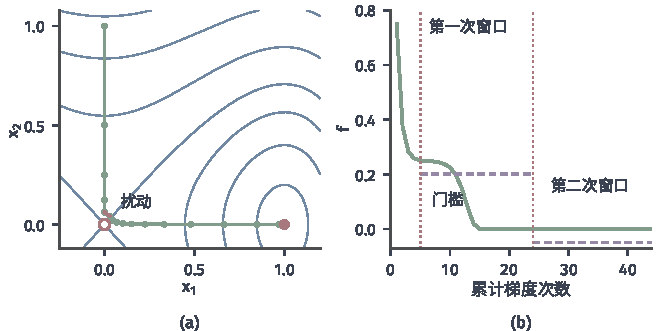
\includegraphics[width=112mm]{figures/05-optimization/02-smooth-optimization/matplotlib/saddle-pgd-run/figure.pdf}
  \caption{扰动梯度法在目标~\eqref{eq:saddle-example}上的运行，$T_{\mathrm{w}}=19$，$F=0.05$，$\bm{\xi}=(0.03,-0.02)$。(a)绿线是路径，红色短线是扰动。(b)目标值随累计梯度次数的变化，红色点线是触发扰动的时刻，紫色虚线是各窗口要求达到的门槛。第一次窗口越过门槛，第二次窗口没有。}
  \label{fig:saddle-pgd-run}
\end{BookInlineFigure}

\paragraph{一般目标上的保证}
定理~\ref{thm:saddle-quadratic-escape}只对二次目标成立。目标不是二次时，Hessian会随位置变化，放大过程可能被打断，所以需要Hessian的Lipschitz条件来控制窗口内的偏差。参数按下面的方式联合选取时，有如下保证\scite{jin2017escape}。

\begin{theorem}[扰动梯度法的高概率保证]
 \label{thm:saddle-pgd}
 设$f$下有界，$\nabla f$是$L$-Lipschitz的，$\nabla^2f$是$M$-Lipschitz的，$\Delta_f=f(\bm{x}^{(0)})-f_{\inf}$，$\varepsilon\leq L^2/M$。取$\alpha=1/L$，半径$r$、窗口$T_{\mathrm{w}}$和门槛$F$按$L,M,\varepsilon,\delta,n,\Delta_f$确定，则至少以$1-\delta$的概率，扰动梯度法返回的点满足
 \begin{equation}
  \lVert\nabla f(\tilde{\bm{x}})\rVert_2\leq\varepsilon,\qquad
  \lambda_{\min}\bigl(\nabla^2f(\tilde{\bm{x}})\bigr)\geq-\sqrt{M\varepsilon},
  \label{eq:saddle-pgd-guarantee}
 \end{equation}
 所用梯度次数为$\tilde O\bigl(L\Delta_f/\varepsilon^2\bigr)$，$\tilde O$隐去了$n,1/\delta,L,M,\Delta_f,1/\varepsilon$的多项对数因子。
\end{theorem}

证明的核心比二次情形多了一个技巧。不能再按特征分量独立讨论，于是考虑两条从窄带两侧出发、只在$\bm{q}_1$方向相差$2w$的迭代序列，用Hessian的Lipschitz条件证明它们的差在窗口内按指数增长，因此两条序列至少有一条离开基点足够远，目标也因此下降足够多。这说明“卡住”的初值不可能在$\bm{q}_1$方向上有大于$2w$的宽度，窄带的宽度得到了控制。完整论证篇幅较长，读者可查阅\scite{jin2017escape}。

定理对参数的要求是实质性的。扰动半径、窗口长度和门槛必须与$L$、$M$、$\varepsilon$和目标下降总量匹配。这里要区分两件事：结论说的是以高概率到达式~\eqref{eq:saddle-pgd-guarantee}定义的点，而不是找到局部极小点，更不是全局最优解。

\paragraph{严格鞍点的结论不能搬到退化驻点}
上面的论证依赖指数放大。退化驻点上没有负特征值，放大是多项式的。比较两个一元函数，步长取$\alpha=\tfrac12$：
\[
 -\frac12y^2:\quad y^{(t+1)}=\frac32y^{(t)};\qquad
 -\frac14y^4:\quad y^{(t+1)}=y^{(t)}+\frac12\bigl(y^{(t)}\bigr)^3.
\]

前者每步放大常数倍，从$y^{(0)}$到$0.5$只要$\log_{1.5}(0.5/y^{(0)})$步。后者可以用微分方程估计：$\mathrm{d}y/\mathrm{d}t\approx\tfrac12y^3$给出$1/y^2$随$t$线性减小，所需步数约为$1/(y^{(0)})^2$。从$y^{(0)}=0.01$出发，两者的实际步数分别是$10$和$10002$。图~\ref{fig:saddle-degenerate-escape}比较了这两种依赖。

\begin{BookInlineFigure}
  \centering
  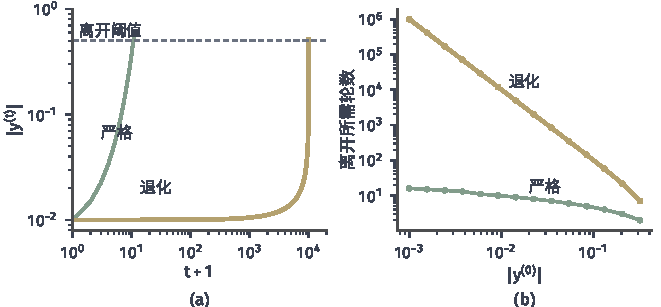
\includegraphics[width=112mm]{figures/05-optimization/02-smooth-optimization/matplotlib/saddle-degenerate-escape/figure.pdf}
  \caption{严格鞍点（绿，$-y^2/2$）与退化驻点（黄，$-y^4/4$）上步长$1/2$的梯度下降。(a)从$y^{(0)}=0.01$出发的$\lvert y^{(t)}\rvert$，虚线是离开阈值$0.5$。(b)离开所需轮数随初值大小的变化，严格鞍点按对数增长，退化驻点按$1/(y^{(0)})^2$增长。}
  \label{fig:saddle-degenerate-escape}
\end{BookInlineFigure}

在一个由$x_1^2-x_2^4$描述的退化鞍点上，扰动梯度法的窗口$T_{\mathrm{w}}$按严格鞍点设计，时间内分量几乎不长，窗口结束时目标没有明显下降，算法就返回基点。这并不违反定理~\ref{thm:saddle-pgd}：基点的$\lambda_{\min}=0\geq-\sqrt{M\varepsilon}$，它满足定理宣称的条件，只是这个条件本来就不排除退化鞍点。

\subsection{利用非正定模型}
\label{sec:saddle-indefinite-model}

二阶方法手里本来就有曲率矩阵。第~\ref{chap:second-order-methods}章和第~\ref{chap:trust-region}章对不定矩阵采取了两种态度：前者把矩阵修正成正定的，后者保留矩阵原样，用半径把模型关起来。这里比较两种态度在鞍点附近的差别，特别是哪种能利用负曲率。

\paragraph{信赖域模型怎样使用负曲率}
回顾第~\ref{chap:trust-region}章的子问题：
\begin{equation}
 \min_{\lVert\bm{p}\rVert_2\leq\Delta}\ m(\bm{p})=f(\bm{x})+\langle\bm{g},\bm{p}\rangle+\frac12\bm{p}^\top\bm{B}\bm{p}.
 \label{eq:saddle-tr-subproblem}
\end{equation}
$\bm{p}$是全局解的充要条件是存在$\lambda\geq0$，使
\begin{equation}
 (\bm{B}+\lambda\bm{I})\bm{p}=-\bm{g},\qquad
 \bm{B}+\lambda\bm{I}\succeq\bm{0},\qquad
 \lambda\bigl(\Delta-\lVert\bm{p}\rVert_2\bigr)=0.
 \label{eq:saddle-tr-optimality}
\end{equation}

第二个条件说明$\lambda\geq-\lambda_{\min}(\bm{B})$。所以$\bm{B}$不定时$\lambda>0$，解一定在边界上：模型沿负曲率方向一直下降，直到碰上半径。这里没有把任何曲率改成正值，负曲率被直接转化成一个长度为$\Delta$的步。

在原点取$\bm{B}=\operatorname{diag}(-1,1)$，$\Delta=\tfrac12$，$\bm{g}=\bm{0}$。条件~\eqref{eq:saddle-tr-optimality}给出$\lambda=1$，第一个方程$(\bm{B}+\bm{I})\bm{p}=\bm{0}$只约束$p_2=0$，于是
\[
 \bm{p}=\begin{bmatrix}\pm\tfrac12\\0\end{bmatrix},\qquad
 m(\bm{0})-m(\bm{p})=\frac18.
\]

代回目标，实际下降和两者之比分别是
\[
 f(\bm{0})-f\bigl(\tfrac12,0\bigr)=\frac14-\frac{9}{64}=0.1094,\qquad
 \rho=\frac{0.1094}{0.125}\approx0.875.
\]
这一步可以接受。梯度精确为零，信赖域仍然走出了一大步，这是只靠梯度的方法做不到的。

\paragraph{修正Hessian的用途不同}
第~\ref{chap:second-order-methods}章的修正让矩阵变成$\bm{B}=\bm{H}+\bm{E}\succ\bm{0}$，解$\bm{B}\bm{d}=-\bm{g}$，目的是得到下降方向，让线搜索有效。这时$\bm{g}=\bm{0}$意味着$\bm{d}=\bm{0}$，算法原地不动。

$\bm{g}$很小但不为零时，以谱修正为例，方向沿$\bm{q}_i$的分量是$-\langle\bm{g},\bm{q}_i\rangle/\lvert\lambda_i\rvert$，长度正比于梯度，鞍点附近很短。下面在点$(0.01,0.0625)$上比较两者。由式~\eqref{eq:saddle-example-derivatives}，该点的数据是
\[
 \bm{g}\approx\begin{bmatrix}-0.0100\\0.0625\end{bmatrix},\qquad
 \bm{H}\approx\operatorname{diag}(-0.9997,1).
\]

谱修正取绝对值，得到的方向和$\Delta=\tfrac12$时子问题的解分别是
\[
 \bm{d}\approx\begin{bmatrix}0.0100\\-0.0625\end{bmatrix},\qquad
 \bm{p}\approx\begin{bmatrix}0.4990\\-0.0309\end{bmatrix}.
\]

子问题的$\lambda\approx1.020$，预测下降$0.1309$，实际下降$0.1142$，$\rho\approx0.872$，接受。修正方向沿$x_1$的分量只有子问题解的约$2\%$。图~\ref{fig:saddle-tr-modified}(a)画出了这两个方向，(b)比较后续运行：修正方法配回溯时，$x_1$大约每轮翻一倍，要$6$轮才接近$0.77$；信赖域$3$轮之内就到了谷底附近，其间有一次拒绝。

\begin{BookInlineFigure}
  \centering
  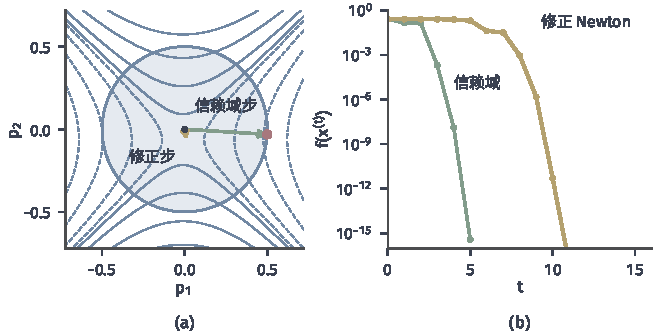
\includegraphics[width=112mm]{figures/05-optimization/02-smooth-optimization/matplotlib/saddle-tr-modified/figure.pdf}
  \caption{点$(0.01,0.0625)$处的比较。(a)蓝线是二次模型的等高线（虚线为负值），浅蓝圆盘半径$\Delta=1/2$，绿色箭头指向子问题的解（红点），黄色短箭头是谱修正方向。(b)从该点出发目标值随轮数的变化，绿线是精确求解子问题的信赖域，黄线是谱修正加Armijo回溯。}
  \label{fig:saddle-tr-modified}
\end{BookInlineFigure}

\paragraph{梯度与负曲率方向正交时}
最能说明两种方法差别的是$\langle\bm{g},\bm{q}_1\rangle=0$的情形。在点$(0,0.0625)$，梯度是$(0,0.0625)$，与$\bm{e}_1$正交。此时条件~\eqref{eq:saddle-tr-optimality}的第一行变成$(\lambda-1)p_1=0$，半正定条件要求$\lambda\geq1$。取$\lambda=1$，第二行和球面条件给出
\[
 p_2=-\frac{0.0625}{1+1}=-0.03125,\qquad
 p_1=\pm\sqrt{\Delta^2-p_2^2}\approx\pm0.4990.
\]

这是第~\ref{chap:trust-region}章所说的困难情形：$\bm{B}+\lambda\bm{I}$奇异，方程本身不能确定$p_1$，要沿$\bm{q}_1$方向补一个分量才到达边界。这一步的预测下降是$0.1260$，$\rho\approx0.877$。

截断共轭梯度却看不到$\bm{e}_1$。它的迭代只在由$\bm{g}$生成的Krylov子空间中进行，这里就是$x_2$轴，第一步就到达$(0,-0.0625)$，残差为零而停止，预测下降只有约$0.002$。图~\ref{fig:saddle-tr-hard-case}(a)是这个点上的模型，(b)是从$(0,1)$出发的运行。截断共轭梯度第一步到达原点，$\bm{g}=\bm{0}$，算法宣布完成。精确子问题第一步是$(0.866,-0.5)$，比值$\rho=0.8125$，第二步到达$(1.039,0)$。

\begin{BookInlineFigure}
  \centering
  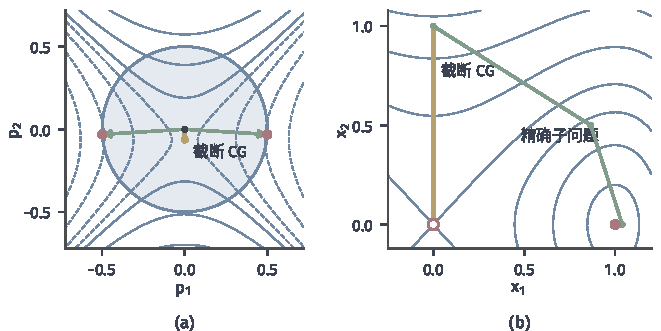
\includegraphics[width=112mm]{figures/05-optimization/02-smooth-optimization/matplotlib/saddle-tr-hard-case/figure.pdf}
  \caption{困难情形。(a)点$(0,0.0625)$处的模型（蓝线）与半径$1/2$的圆盘，两个红点是子问题的全局解，黄线是截断共轭梯度的结果，它留在$p_2$轴上。(b)从$(0,1)$出发、$\Delta^{(0)}=1$的运行：绿线精确求解子问题，黄线用截断共轭梯度，一步到达鞍点后停止。}
  \label{fig:saddle-tr-hard-case}
\end{BookInlineFigure}

这里要记住：算出的步是否利用负曲率，由子问题的求解方式决定。使用截断共轭梯度的信赖域，在$\bm{g}$恰好避开$\bm{q}_1$时和修正方法一样看不见负曲率。

\paragraph{后续保证的差别}
第~\ref{chap:trust-region}章的二阶保证要求候选步的模型下降满足下面的条件，其中$\lambda_-=\max\{0,-\lambda_{\min}\}$，$c_2>0$是常数：
\[
 \operatorname{pred}(\bm{p})\geq c_2\lambda_-\Delta^2.
\]
由此得到
\begin{equation}
 \liminf_{t\to\infty}\max\bigl\{\lVert\bm{g}^{(t)}\rVert_2,\ \lambda_-^{(t)}\bigr\}=0.
 \label{eq:saddle-tr-liminf}
\end{equation}
精确解$c_2=\tfrac12$，满足这一条；只有一阶信息的步不满足，保证也就退回到$\bm{g}^{(t)}\to\bm{0}$。

不想精确求解时，可以把第~\ref{sec:saddle-detection}节的检测嫁接进来。设检测给出$\bm{v}$，$\bm{v}^\top\bm{B}\bm{v}\leq-\gamma$，选符号使$\langle\bm{g},\bm{v}\rangle\leq0$，把$\Delta\bm{v}$作为候选步，它的预测下降是
\[
 m(\bm{0})-m(\Delta\bm{v})=-\Delta\langle\bm{g},\bm{v}\rangle-\frac{\Delta^2}{2}\bm{v}^\top\bm{B}\bm{v}\geq\frac12\gamma\Delta^2.
\]

只要$\gamma$不小于$\lambda_-$的一个固定倍数，例如$\gamma\geq\tfrac12\lambda_-$，就得到$c_2=\tfrac14$，第~\ref{chap:trust-region}章的论证可以照搬。当然这样一来保证就带上了检测的失败概率。表~\ref{tab:saddle-model-compare}总结了各种做法的区别。

\begin{BookInlineTable}
  \centering
  \begin{tabular}{@{}lll@{}}
    \toprule
    做法 & 在$\bm{g}=\bm{0}$的鞍点 & 结论\\
    \midrule
    修正Hessian加线搜索 & 不动 & $\bm{g}^{(t)}\to\bm{0}$\\
    信赖域，Cauchy步或截断CG & 不动 & $\bm{g}^{(t)}\to\bm{0}$\\
    信赖域，精确子问题 & 走到边界 & 式~\eqref{eq:saddle-tr-liminf}\\
    信赖域，加入负曲率检测 & 走到边界 & 同上，带失败概率\\
    \bottomrule
  \end{tabular}
  \caption{几种处理不定矩阵的做法。式~\eqref{eq:saddle-tr-liminf}的二阶结论只说明子列满足二阶必要条件，不说明极限点是局部极小点。}
  \label{tab:saddle-model-compare}
\end{BookInlineTable}

总之，修正Hessian解决的是“方向要下降”，保留不定模型解决的是“负曲率要被利用”。两者的出发点不同，后续能给出的保证也不同，不应混为一谈。


\section{停止条件与计算成本}
\label{sec:saddle-stopping}

算法什么时候可以停，一次运行究竟可以报告什么？第~\ref{chap:smooth-foundations}章要求比较算法之前固定三件事：误差标准、返回哪个点、计算量怎样累计。这里把这三件事放到二阶情形下落实。

\paragraph{两个容差}
只有一个梯度容差无法排除鞍点，所以要同时控制梯度大小和Hessian最小特征值的负部。

\begin{definition}[近似二阶驻点]
 \label{def:saddle-approximate}
 给定$\varepsilon_g>0$，$\varepsilon_H>0$，若点$\bm{x}$满足
 \begin{equation}
  \lVert\nabla f(\bm{x})\rVert_2\leq\varepsilon_g,\qquad
  \lambda_{\min}\bigl(\nabla^2f(\bm{x})\bigr)\geq-\varepsilon_H,
  \label{eq:saddle-approximate}
 \end{equation}
 就称它为$(\varepsilon_g,\varepsilon_H)$\term{近似二阶驻点}（approximate second-order stationary point）。
\end{definition}

例中$\varepsilon_g=0.1$，$\varepsilon_H\approx0.775$。点$(0,0.0625)$的梯度范数$0.0625$通过了第一个条件，$\lambda_{\min}=-1$没有通过第二个。点$(0.9686,0.0039)$的梯度范数$0.060$，$\lambda_{\min}=1$，两个都通过。图~\ref{fig:saddle-tolerance-plane}(a)把表~\ref{tab:saddle-nc-run}的运行画在这两个量组成的平面上，(b)在变量空间中画出了两种验收区的差别。

\begin{BookInlineFigure}
  \centering
  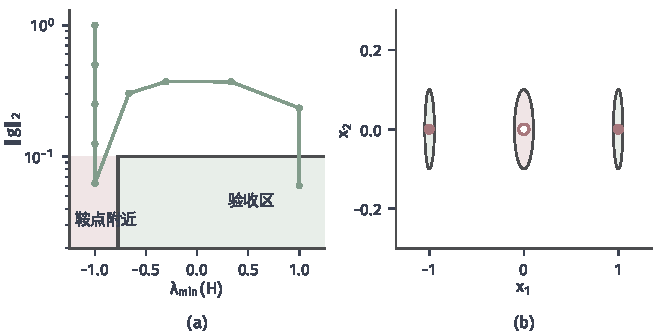
\includegraphics[width=112mm]{figures/05-optimization/02-smooth-optimization/matplotlib/saddle-tolerance-plane/figure.pdf}
  \caption{两个容差的验收区，$\varepsilon_g=0.1$，$\varepsilon_H\approx0.775$。(a)横轴是$\lambda_{\min}(\bm{H})$，纵轴是$\lVert\bm{g}\rVert_2$（对数坐标），绿色矩形是验收区，粗线是边界，浅红区梯度合格而曲率不合格，折线是表~\ref{tab:saddle-nc-run}的运行。(b)目标~\eqref{eq:saddle-example}上$\lVert\nabla f\rVert_2\leq\varepsilon_g$的三块区域，鞍点周围的一块（浅红）不满足曲率条件，只有两侧（浅绿）满足全部条件。}
  \label{fig:saddle-tolerance-plane}
\end{BookInlineFigure}

\paragraph{两个容差怎样搭配}
两个容差不是独立的。式~\eqref{eq:saddle-approximate}对目标下降的限制可以由三次上界直接算出：设半径$r$的球落在引理~\ref{lem:saddle-cubic}的凸集内，对$\lVert\bm{p}\rVert_2\leq r$，由该引理和式~\eqref{eq:saddle-approximate}，
\begin{equation}
 f(\bm{x}+\bm{p})\geq f(\bm{x})-\varepsilon_gr-\frac12\varepsilon_Hr^2-\frac{M}{6}r^3.
 \label{eq:saddle-tolerance-drop}
\end{equation}

三项分别来自梯度、负曲率和Hessian的变化。让三项同量级，由后两项得到$r\sim\varepsilon_H/M$，代入前两项得到$\varepsilon_g\sim\varepsilon_H^2/M$，于是自然的搭配是
\begin{equation}
 \varepsilon_H=\sqrt{M\varepsilon_g}.
 \label{eq:saddle-tolerance-scale}
\end{equation}

此时取$r=\sqrt{\varepsilon_g/M}$，式~\eqref{eq:saddle-tolerance-drop}的三项合计给出
\[
 f(\bm{x}+\bm{p})\geq f(\bm{x})-\frac{5}{3}\frac{\varepsilon_g^{3/2}}{\sqrt{M}}.
\]
这就是通过验收的点能保证的事：在半径$r$的球内，目标至多还能下降这么多。

\paragraph{通过验收不等于局部极小}
式~\eqref{eq:saddle-tolerance-drop}只限制了小球内的下降幅度，并不排除下降。$x_1^2-x_2^4$在原点梯度和Hessian的负部都是零，对任意容差都通过验收，而原点不是局部极小点，甚至这个目标没有下界。

容差取得过大也会放过严格鞍点。例中若$\varepsilon_H=2$，原点的$\lambda_{\min}=-1$就能通过。

所以报告结果时，应该写“近似二阶驻点，容差为$(\varepsilon_g,\varepsilon_H)$”，不写“找到了局部极小点”，更不写“找到了最优解”。

\paragraph{返回哪个点}
验收条件是针对具体的点的，所以返回的点必须就是验收的那个点。负曲率算法直接返回验收通过的$\bm{x}^{(t)}$。扰动梯度法返回窗口开始之前保存的基点$\tilde{\bm{x}}$，因为梯度小的判断是在基点上作出的，窗口结束时的点没有经过判断。

\paragraph{要累计哪些计算量}
这一节的成本有四类，单位要分开：梯度次数，Hessian向量积次数，矩阵分解次数，以及扰动窗口的梯度次数。

扰动窗口的次数也有上界。除了最后一次之外，每次窗口都使目标下降至少$F$，所以窗口总数不超过$\Delta_f/F+1$。例中上界是$16$次窗口，共$304$次梯度，实际只用了$2$次窗口。每次窗口都有失败的可能，失败概率要像下面的检测一样累计。

检测的失败概率也要累计。负曲率算法可能进行多次检测，任何一次“未找到”判断错误都会使算法提前停止。若检测次数不超过$K$，每次失败概率取$\delta/K$，由并的概率不等式，总失败概率不超过$\delta$，代价只是对数因子$\ln(K/\delta)$。

检测有两个方向，失败只发生在“未找到”的方向上。每次发现负曲率都是确定的，所以不需要担心算法走错一步。真正的风险是错误地宣布停止。下面把这些成本组合起来。

取$\gamma_0=\varepsilon_H/2$，检测精度$\varepsilon_H/2$，由式~\eqref{eq:saddle-no-find}，未找到时$\lambda_{\min}\geq-\varepsilon_H$。把$\varepsilon_H=\sqrt{M\varepsilon}$代入定理~\ref{thm:saddle-nc-count}，负曲率步的次数不超过
\begin{equation}
 K=\frac{12\sqrt{M}\,\Delta_f}{\varepsilon^{3/2}}.
 \label{eq:saddle-detect-count}
\end{equation}

用Lanczos方法时每次检测$O(\sqrt{L/\varepsilon_H}\,\ln(nK/\delta))$次乘积，总数是
\begin{equation}
 O\Bigl(\frac{\sqrt{L}\,M^{1/4}\Delta_f}{\varepsilon^{7/4}}\ln\frac{nK}{\delta}\Bigr).
 \label{eq:saddle-lanczos-total}
\end{equation}
这个量对$1/\varepsilon$的幂次比梯度步的$O(L\Delta_f/\varepsilon^2)$低$1/4$，所以在小容差下乘积的总量不会超过梯度的总量。换成幂迭代时，每次检测$O((L/\varepsilon_H)\ln(nK/\delta))$次乘积，总数变成$O((L\Delta_f/\varepsilon^2)\ln(nK/\delta))$，与梯度步同阶。

表~\ref{tab:saddle-cost-bounds}汇总了各种做法在最坏情形下的曲率成本，表中$\varepsilon_g=\varepsilon$，$\varepsilon_H=\sqrt{M\varepsilon}$。前三行的梯度次数都不超过$2L\Delta_f/\varepsilon^2$加检测带来的少量读取，扰动梯度法的梯度次数是$\tilde O(L\Delta_f/\varepsilon^2)$，这里的$\tilde O$隐去了对数因子。

\begin{BookInlineTable}
  \centering
  \begin{tabular}{@{}lll@{}}
    \toprule
    方法 & 曲率读取（梯度次数见正文） & 保证\\
    \midrule
    梯度下降 & 无 & 一阶，确定\\
    负曲率步，特征分解 & $O(\sqrt{M}\Delta_f/\varepsilon^{3/2})$次分解 & 二阶，确定\\
    负曲率步，Lanczos & 式~\eqref{eq:saddle-lanczos-total}的次数 & 二阶，$\geq1-\delta$\\
    扰动梯度法 & 无 & 二阶，$\geq1-\delta$\\
    信赖域，精确子问题 & $O(\varepsilon^{-2})$轮，每轮一次分解 & 二阶，确定\\
    \bottomrule
  \end{tabular}
  \caption{达到式~\eqref{eq:saddle-approximate}的最坏情形成本，“二阶”指近似二阶驻点，“$\geq1-\delta$”指成立的概率。信赖域一行由第~\ref{chap:trust-region}章的轮数估计得到，并依赖半径下界中的常数。}
  \label{tab:saddle-cost-bounds}
\end{BookInlineTable}

\paragraph{一次实际运行的账}
上界比较的是最坏情形，单次运行要按实际次数报告。表~\ref{tab:saddle-run-cost}是从$(0,1)$出发、$\varepsilon_g=0.1$、$\varepsilon_H\approx0.775$时各方法的实际计数。

\begin{BookInlineTable}
  \centering
  \begin{tabular}{@{}lrlcc@{}}
    \toprule
    方法 & 梯度 & 曲率读取 & 返回点 & 通过\\
    \midrule
    梯度下降 & $5$ & 无 & $(0,\ 0.0625)$ & 否\\
    谱修正Newton & $2$ & $1$次分解 & $(0,\ 0)$ & 否\\
    信赖域，截断CG & $2$ & $1$次乘积 & $(0,\ 0)$ & 否\\
    负曲率步，特征分解 & $10$ & $2$次分解 & $(0.969,\ 0.004)$ & 是\\
    负曲率步，幂迭代 & $11$ & $151$次乘积 & $(0.981,\ -0.001)$ & 是\\
    扰动梯度法 & $44$ & 无 & $(1.000,\ 0.000)$ & 是\\
    信赖域，精确子问题 & $3$ & $3$次分解 & $(1.039,\ 0)$ & 是\\
    \bottomrule
  \end{tabular}
  \caption{从$(0,1)$出发的实际计数，“通过”指是否满足式~\eqref{eq:saddle-approximate}。幂迭代用$L=2$，随机起点的种子固定为$0$，检测精度$\varepsilon_H/2$，失败概率$\delta=0.05$（两次检测的总失败概率约$0.1$），上限由式~\eqref{eq:saddle-power-rounds}算得$149$次。}
  \label{tab:saddle-run-cost}
\end{BookInlineTable}

表中前三行的算法都很便宜，但报告的点是鞍点。它们的共同问题是起点在$x_2$轴上，梯度始终看不到$x_1$方向。负曲率步用幂迭代时，第一次检测只用$2$次乘积就找到了方向，其余$149$次全部花在最后一次“未找到”的确认上。

这说明确认“没有负曲率”才是最贵的一步，手段越便宜，这一步越依赖概率。实际程序常常把上限设得比理论值小，这时要如实报告：这样的结果只是经验判断，不再带有定理~\ref{thm:saddle-power}的概率保证。

\paragraph{一次报告应该包含什么}
把三件事落实到底，一次运行的结论可以写成这样：对目标~\eqref{eq:saddle-example}，从$(0,1)$出发，用幂迭代检测负曲率的交替算法，返回点满足$\lVert\nabla f\rVert_2\leq0.1$；未找到负曲率的判断由$149$次乘积支持，至少以$0.9$的概率有$\lambda_{\min}\geq-0.775$；共用$11$次梯度和$151$次Hessian向量积。

这样的报告说清了误差标准（两个容差）、返回的点（验收通过的点）、成本（分类计数）和可信度（失败概率）。它没有声称局部极小，也没有声称全局最优，这两件事本章的方法都保证不了。


\section{本章小结}
\label{sec:saddle-summary}

本章从一个具体的疑问出发：梯度很小的点算不算找到了解。梯度小只说明一阶变化弱，山口和谷底都满足这一点。

驻点按二阶信息分成严格鞍点和二阶驻点。负曲率是确凿的证据，说明这里还能下降；Hessian正定也是确凿的证据，说明这里是局部极小点。半正定而奇异的情形，二阶信息无法判断，$x_1^2+x_2^4$与$x_1^2-x_2^4$就是例子。即使确实是局部极小点，也不说明是全局最优解。

负曲率可以只靠Hessian向量积发现。幂迭代和Lanczos方法从随机起点出发，找到方向时的结论是确定的，未找到时的结论带有失败概率，检测误差和差分误差都要计入。

离开鞍点有三种机制，它们的条件和结论各不相同。

\begin{BookInlineTable}
  \centering
  \begin{tabular}{@{}lll@{}}
    \toprule
    机制 & 需要的条件 & 结论\\
    \midrule
    负曲率步 & 方向、Hessian Lipschitz & 每步确定下降$\frac{2\gamma^3}{3M^2}$\\
    扰动梯度法 & 梯度、$L$、$M$、随机扰动 & 高概率到达近似二阶驻点\\
    不定模型 & 子问题使用负曲率 & 二阶必要条件的下极限\\
    \bottomrule
  \end{tabular}
  \caption{三种离开鞍点的机制。修正Hessian只为得到下降方向，它的保证停留在一阶。}
  \label{tab:saddle-summary}
\end{BookInlineTable}

检测精度和离开机制共同决定了能够声称的保证。停止时用两个容差描述近似二阶驻点，$\varepsilon_H=\sqrt{M\varepsilon_g}$是自然的搭配，它限制了小球内还能下降多少，但不说明这个点是局部极小点。计算量要把梯度、Hessian向量积、分解和扰动窗口分开统计，并报告确定性保证或相应的失败概率。

到这里，光滑优化中的方向、步长、曲率和成本的框架已经完整。这些方法都假设梯度存在。下一部分研究目标在某些点没有普通梯度时，怎样改用次微分和邻近结构。


